\documentclass[../thesis.tex]{subfiles}

\usepackage{wrapfig}
\usepackage{cite}
% \usepackage{natbib}
% \usepackage[round]{natbib}

\usepackage{amsfonts}       % blackboard math symbols
\usepackage{nicefrac}       % compact symbols for 1/2, etc.
\usepackage{microtype}      % microtypography
\usepackage{amsmath}
\usepackage{tikz}
\usepackage{amsthm}
\usepackage{amssymb}
\usetikzlibrary{positioning}
\usepackage{mathtools}

\newtheorem{theorem}{Theorem}[section]
\newtheorem{assumption}{Assumption}[section]
\newtheorem{proposition}{Proposition}[section]
\newtheorem{definition}{Definition}[section]
\newtheorem{corollary}{Corollary}[theorem]
\newtheorem{lemma}{Lemma}[theorem]
% \newtheorem{corollary}{Corollary}[proposition]
\newtheorem{definition1}{Definition}[section]



% %% editing comment
\newcommand{\cmt}[1]{{\footnotesize\textcolor{red}{#1}}}
\newcommand{\cmto}[1]{{\footnotesize\textcolor{orange}{#1}}}
\newcommand{\note}[1]{\cmt{Note: #1}}
\newcommand{\todo}[1]{\cmt{TO-DO: #1}}
\newcommand{\question}[1]{\cmto{Question: #1}}
\newcommand{\sergey}[1]{{\footnotesize\textcolor{blue}{Sergey: #1}}}
\newcommand{\ak}[1]{{\textcolor{red}{#1}}}
\newcommand{\edits}[1]{\textcolor{red}{#1}}

%% abbreviations
\newcommand{\x}{\mathbf{x}}
\newcommand{\z}{\mathbf{z}}
\newcommand{\y}{\mathbf{y}}
\newcommand{\w}{\mathbf{w}}
\newcommand{\data}{\mathcal{D}}

\newcommand{\etal}{{et~al.}\ }
\newcommand{\eg}{e.g.\ }
\newcommand{\ie}{i.e.\ }
\newcommand{\nth}{\text{th}}
\newcommand{\pr}{^\prime}
\newcommand{\tr}{^\mathrm{T}}
\newcommand{\inv}{^{-1}}
\newcommand{\pinv}{^{\dagger}}
\newcommand{\real}{\mathbb{R}}
\newcommand{\gauss}{\mathcal{N}}
\newcommand{\norm}[1]{\left|#1\right|}
\newcommand{\trace}{\text{tr}}

%% specifics for the paper
\newcommand{\reward}{r}
\newcommand{\policy}{\pi}
\newcommand{\mdp}{\mathcal{M}}
\newcommand{\states}{\mathcal{S}}
\newcommand{\actions}{\mathcal{A}}
\newcommand{\observations}{\mathcal{O}}
\newcommand{\transitions}{T}
\newcommand{\initstate}{d_0}
\newcommand{\freq}{d}
\newcommand{\obsfunc}{E}
\newcommand{\initial}{\mathcal{I}}
\newcommand{\horizon}{H}
\newcommand{\rewardevent}{R}
\newcommand{\probr}{p_\rewardevent}
\newcommand{\metareward}{\bar{\reward}}
\newcommand{\discount}{\gamma}
\newcommand{\behavior}{{\pi_\beta}}
\newcommand{\bellman}{\mathcal{B}}
\newcommand{\qparams}{\phi}
\newcommand{\qparamset}{\Phi}
\newcommand{\qset}{\mathcal{Q}}
\newcommand{\batch}{B}
\newcommand{\qfeat}{\mathbf{f}}
\newcommand{\Qfeat}{\mathbf{F}}
\newcommand{\hatbehavior}{\hat{\pi}_\beta}

\newcommand{\traj}{\tau}

\newcommand{\pihi}{\pi^{\text{hi}}}
\newcommand{\pilo}{\pi^{\text{lo}}}
\newcommand{\ah}{\mathbf{w}}

\newcommand{\proj}{\Pi}

\newcommand{\loss}{\mathcal{L}}
\newcommand{\eye}{\mathbf{I}}

\newcommand{\model}{\hat{p}}

\newcommand{\pimix}{\pi_{\text{mix}}}

\newcommand{\pib}{\bar{\pi}}
\newcommand{\epspi}{\epsilon_{\pi}}
\newcommand{\epsmodel}{\epsilon_{m}}

\newcommand{\return}{\mathcal{R}}

%% math
\newcommand{\cY}{\mathcal{Y}}
\newcommand{\cX}{\mathcal{X}}
\newcommand{\en}{\mathcal{E}}
\newcommand{\be}{\mathbf{e}}
\newcommand{\by}{\mathbf{y}}
\newcommand{\bx}{\mathbf{x}}
\newcommand{\bz}{\mathbf{z}}
\newcommand{\bo}{\mathbf{o}}
\newcommand{\bs}{\mathbf{s}}
\newcommand{\ba}{\mathbf{a}}
\newcommand{\bM}{\mathbf{M}}
\newcommand{\ot}{\bo_t}
\newcommand{\st}{\bs_t}
\newcommand{\at}{\ba_t}
\newcommand{\op}{\mathcal{O}}
\newcommand{\opt}{\op_t}
\newcommand{\kl}{D_\text{KL}}
\newcommand{\tv}{D_\text{TV}}
\newcommand{\ent}{\mathcal{H}}

\newcommand{\bzhi}{\bz^\text{hi}}

\newcommand{\E}{\mathbb{E}}

\newenvironment{repeatedthm}[1]{\@begintheorem{#1}{\unskip}}{\@endtheorem}

% \DeclareMathOperator\supp{supp}



\begin{document}


% \blfootnote{This chapter is based on \cite{kumar2020conservative}, published at NeurIPS 2020, which is joint work with Aurick Zhou, George Tucker, and Sergey Levine.}

\vspace{-0.4cm}
\begin{AIbox}{\large{\textbf{Abstract}}}
\vspace{4mm}
Thus far, we have developed algorithms for learning policies from offline data. In practice, we would often want to instantiate these algorithms in a way that allow them to ingest larger amounts of broad and diverse data to produce performant policies. One way to do so is to train high-capacity neural network value functions and policies with broad offline datasets. In support is the observation that this sort of a recipe is quite effective in supervised learning: despite the massive over-parameterization, deep networks trained via supervised learning are easy to optimize and exhibit excellent generalization. One hypothesis to explain this is that overparameterized deep networks enjoy the benefits of implicit regularization induced by stochastic gradient descent (SGD), which favors parsimonious solutions that generalize well on test inputs. It is reasonable to surmise that deep reinforcement learning (RL) methods could also benefit from this effect. In this chapter, we discuss how the implicit regularization effect of SGD seen in supervised learning could in fact be harmful in the offline deep RL setting, leading to poor generalization and degenerate feature representations. Our theoretical analysis shows that when existing models of implicit regularization are applied to temporal difference learning (TD-learning), the resulting derived regularizer favors degenerate solutions with excessive ``aliasing'', in stark contrast to the supervised learning case. We back up these findings empirically and propose a simple and effective \emph{explicit} regularizer, called \drmethodname, that counteracts this undesirable effect. We then build on this technique to enable, for the first time, a recipe that can train 100 million parameter ResNet models entirely via offline TD-learning to outperform variants of behavioral cloning with heterogeneous data.
\vspace{2mm}
\end{AIbox}


\vspace{-0.2cm}
\section{Introduction}
\vspace{-0.2cm}

Despite being massively over-parameterized, deep neural networks with billions of parameters still learn representations that generalize well when trained with supervised and unsupervised learning approaches. This is despite the classical notions of overfitting when provided with many parameters. A widely held consensus is that deep networks find simple solutions that generalize due to various \emph{implicit} regularization effects~\citep{blanc2020implicit,woodworth2020kernel,arora2018optimization,gunasekar2017implicit,wei2019regularization,li2019towards}. Does this mean that large, over-parameterized networks will also be simpliarly performant for offline RL, scaling and generalizing well as the number of parameters is increased?

In the first part of this chapter, we show that, implicit regularization may lead to poor learned representations when training overparameterized deep network value functions via offline RL. This often manifests as the inability to improve performance with larger deep network models, and in particular, unreliable optimization behavior over the course of offline RL training. While there is already some empirical studies showing that value function training via offline temporal-difference (TD) learning leads to emergence of poor representations~\citep{kumar2021implicit}, our goal in this chapter is to understand the cause in a simpler theoretical model and develop a potential solution. Building on the theoretical framework developed by \citet{blanc2020implicit,damian2021label}, we characterize the implicit regularizer that arises when training deep value functions with offline TD learning. The form of this implicit regularizer implies that offline TD-learning would ``co-adapt'' the learned feature representations at state-action tuples that appear on either side of a Bellman backup.

Practically, we illustrate that this theoretically-predicted co-adaptation phenomenon results in a higher dot product of the features of consecutive state-action tuples learned by the Q-value network~(\Secref{sec:problem}). Training runs that exhibit feature co-adaptation typically converge to poorly performing solutions. Even when Q-values are not overestimated, prolonged training in offline RL can result in performance degradation as feature co-adaptation increases. To mitigate this co-adaptation issue, which arises as a result of implicit regularization, we propose an \emph{explicit regularizer} that we call \drmethodname~(\Secref{sec:method}). While exactly estimating the effects of the theoretically derived implicit regularizer is computationally difficult, \drmethodname\ provides a simple and tractable approximation that mitigates the issues discussed above. In practice, \drmethodname\ amounts to regularizing the features at consecutive state-action pairs to be dissimilar in terms of their dot-product similarity. Empirically, we find that \drmethodname\ prevents previously noted pathologies such as feature rank collapse~\citep{kumar2021implicit}, gives methods that train for longer and improves performance relative to the base offline RL method on benchmark problems.

Building on this approach, in the second part of this chapter, we perform a large-scale empirical study that aims to train a large model via offline conservative Q-learning. Specifically, we train a single policy to play 40 Atari games~\citep{bellemare2013arcade}, similarly to \citet{lee2022multi}, and evaluate performance when the training dataset contains expert trajectories \emph{and} when the data is sub-optimal. This problem is especially challenging because of the diversity of games with their own unique dynamics, reward, visuals, and agent embodiments. Furthermore, the sub-optimal data setting requires the learning algorithm to ``stitch together'' useful segments of sub-optimal trajectories to perform well. Our approach, \textbf{scaled Q-learning}, incorporates a variant of the \drmethodname\ technique which normalizes features instead of regularization to attain the same benefit without needing a hyperparameter, in conjunction with careful neural network architectural design decisions. Scaled Q-learning is able to train upto 80 million parameter ResNet~\citep{he2016resnet} models entirely via offline RL and the performance of our approach follows a power-law relationship between model capacity and performance, similar to various scaling studies in supervised and unsupervised learning. In terms of absolute performance, scaled Q-learning learns policies that attain more than 100\% human-level performance on most of the 40 games, about \textbf{2x} better than prior supervised learning~(SL) approaches for learning from sub-optimal offline data (51\% human-level performance).    

% Our first contribution is the derivation of the implicit regularizer that arises when training deep net value functions via TD learning, and an empirical demonstration that it manifests as \emph{feature co-adaptation} in the offline deep RL setting.
% %, which results in highly similar feature representations for state-action tuples at consecutive time steps. 
% Feature co-adaptation accounts at least in part for some of the challenges of offline deep RL, including degradation of performance with prolonged training. Second, we propose a simple and effective \emph{explicit} regularizer for offline value-based RL, \drmethodname, which minimizes the feature similarity between state-action pairs appearing in a bootstrapping update. \drmethodname\ is inspired by the theoretical derivation of the implicit regularizer, it alleviates co-adaptation and can be easily combined with modern offline RL methods, such as REM~\citep{agarwal2019optimistic}, CQL~\citep{kumar2020conservative}, and BRAC~\citep{wu2019behavior}. Empirically, using \drmethodname\ in conjunction with existing offline RL methods provides about \textbf{60\%} performance improvement on the harder D4RL~\citep{fu2020d4rl} tasks, and \textbf{160\%} and \textbf{25\%} stability gains for REM and CQL, respectively, on offline RL tasks in 17 Atari 2600 games. Additionally, we observe large improvements on image-based robotic manipulation tasks~\citep{singh2020cog}.


\section{DR3: Explicit Regularization For Value-Based Offline RL}

\vspace{-0.3cm}
\section{Implicit Regularization in Deep RL via TD-Learning}
\vspace{-0.3cm}
\label{sec:problem}
While the ``deadly-triad''~\citep{suttonrlbook} suggests that training value function approximators with bootstrapping off-policy can lead to divergence, modern deep RL algorithms have been able to successfully combine these properties~\citep{Hasselt2018DeepRL}. However, making too many TD updates to the Q-function in offline deep RL is known to sometimes lead to performance degradation and unlearning, even for otherwise effective modern algorithms~\citep{fu2019diagnosing, fedus2020revisiting,agarwal2019optimistic,kumar2021implicit}. Such unlearning is not typically observed when training overparameterized models via supervised learning, so what about TD learning is responsible for it? We show that one possible explanation behind this pathology is the implicit regularization induced by minimizing TD error on a deep Q-network. Our theoretical results suggest that this implicit regularization ``co-adapts'' the representations of state-action pairs that appear in a Bellman backup (we will define this more precisely below).
%, and this co-adaptation is exacerbated when utilizing unseen state-action pairs for the Bellman backup. 
%%SL.12.5: I still think we should not talk about "unseen state-action pairs" at this level of abstraction, because no one is going to understand it
% even with algorithms that account for distribution shift. 
%%AK: commented the stuff above because we don't really show this theoretically
Empirically, this typically manifests as ``co-adapted'' features for consecutive state-action tuples, even with specialized TD-learning algorithms that account for distributional shift, and this in turn leads to poor final performance both in theory and in practice. We first provide empirical evidence of this co-adaptation phenomenon in Section~\ref{app:problem_more} (additional evidence in Appendix~\ref{app:more_evidence_coadaptation}) and then theoretically characterize the implicit regularization in TD learning, and discuss how it can explain the co-adaptation phenomenon in Section~\ref{sec:theory}.

\begin{figure}[t]
    \centering
    \vspace{-5pt}
    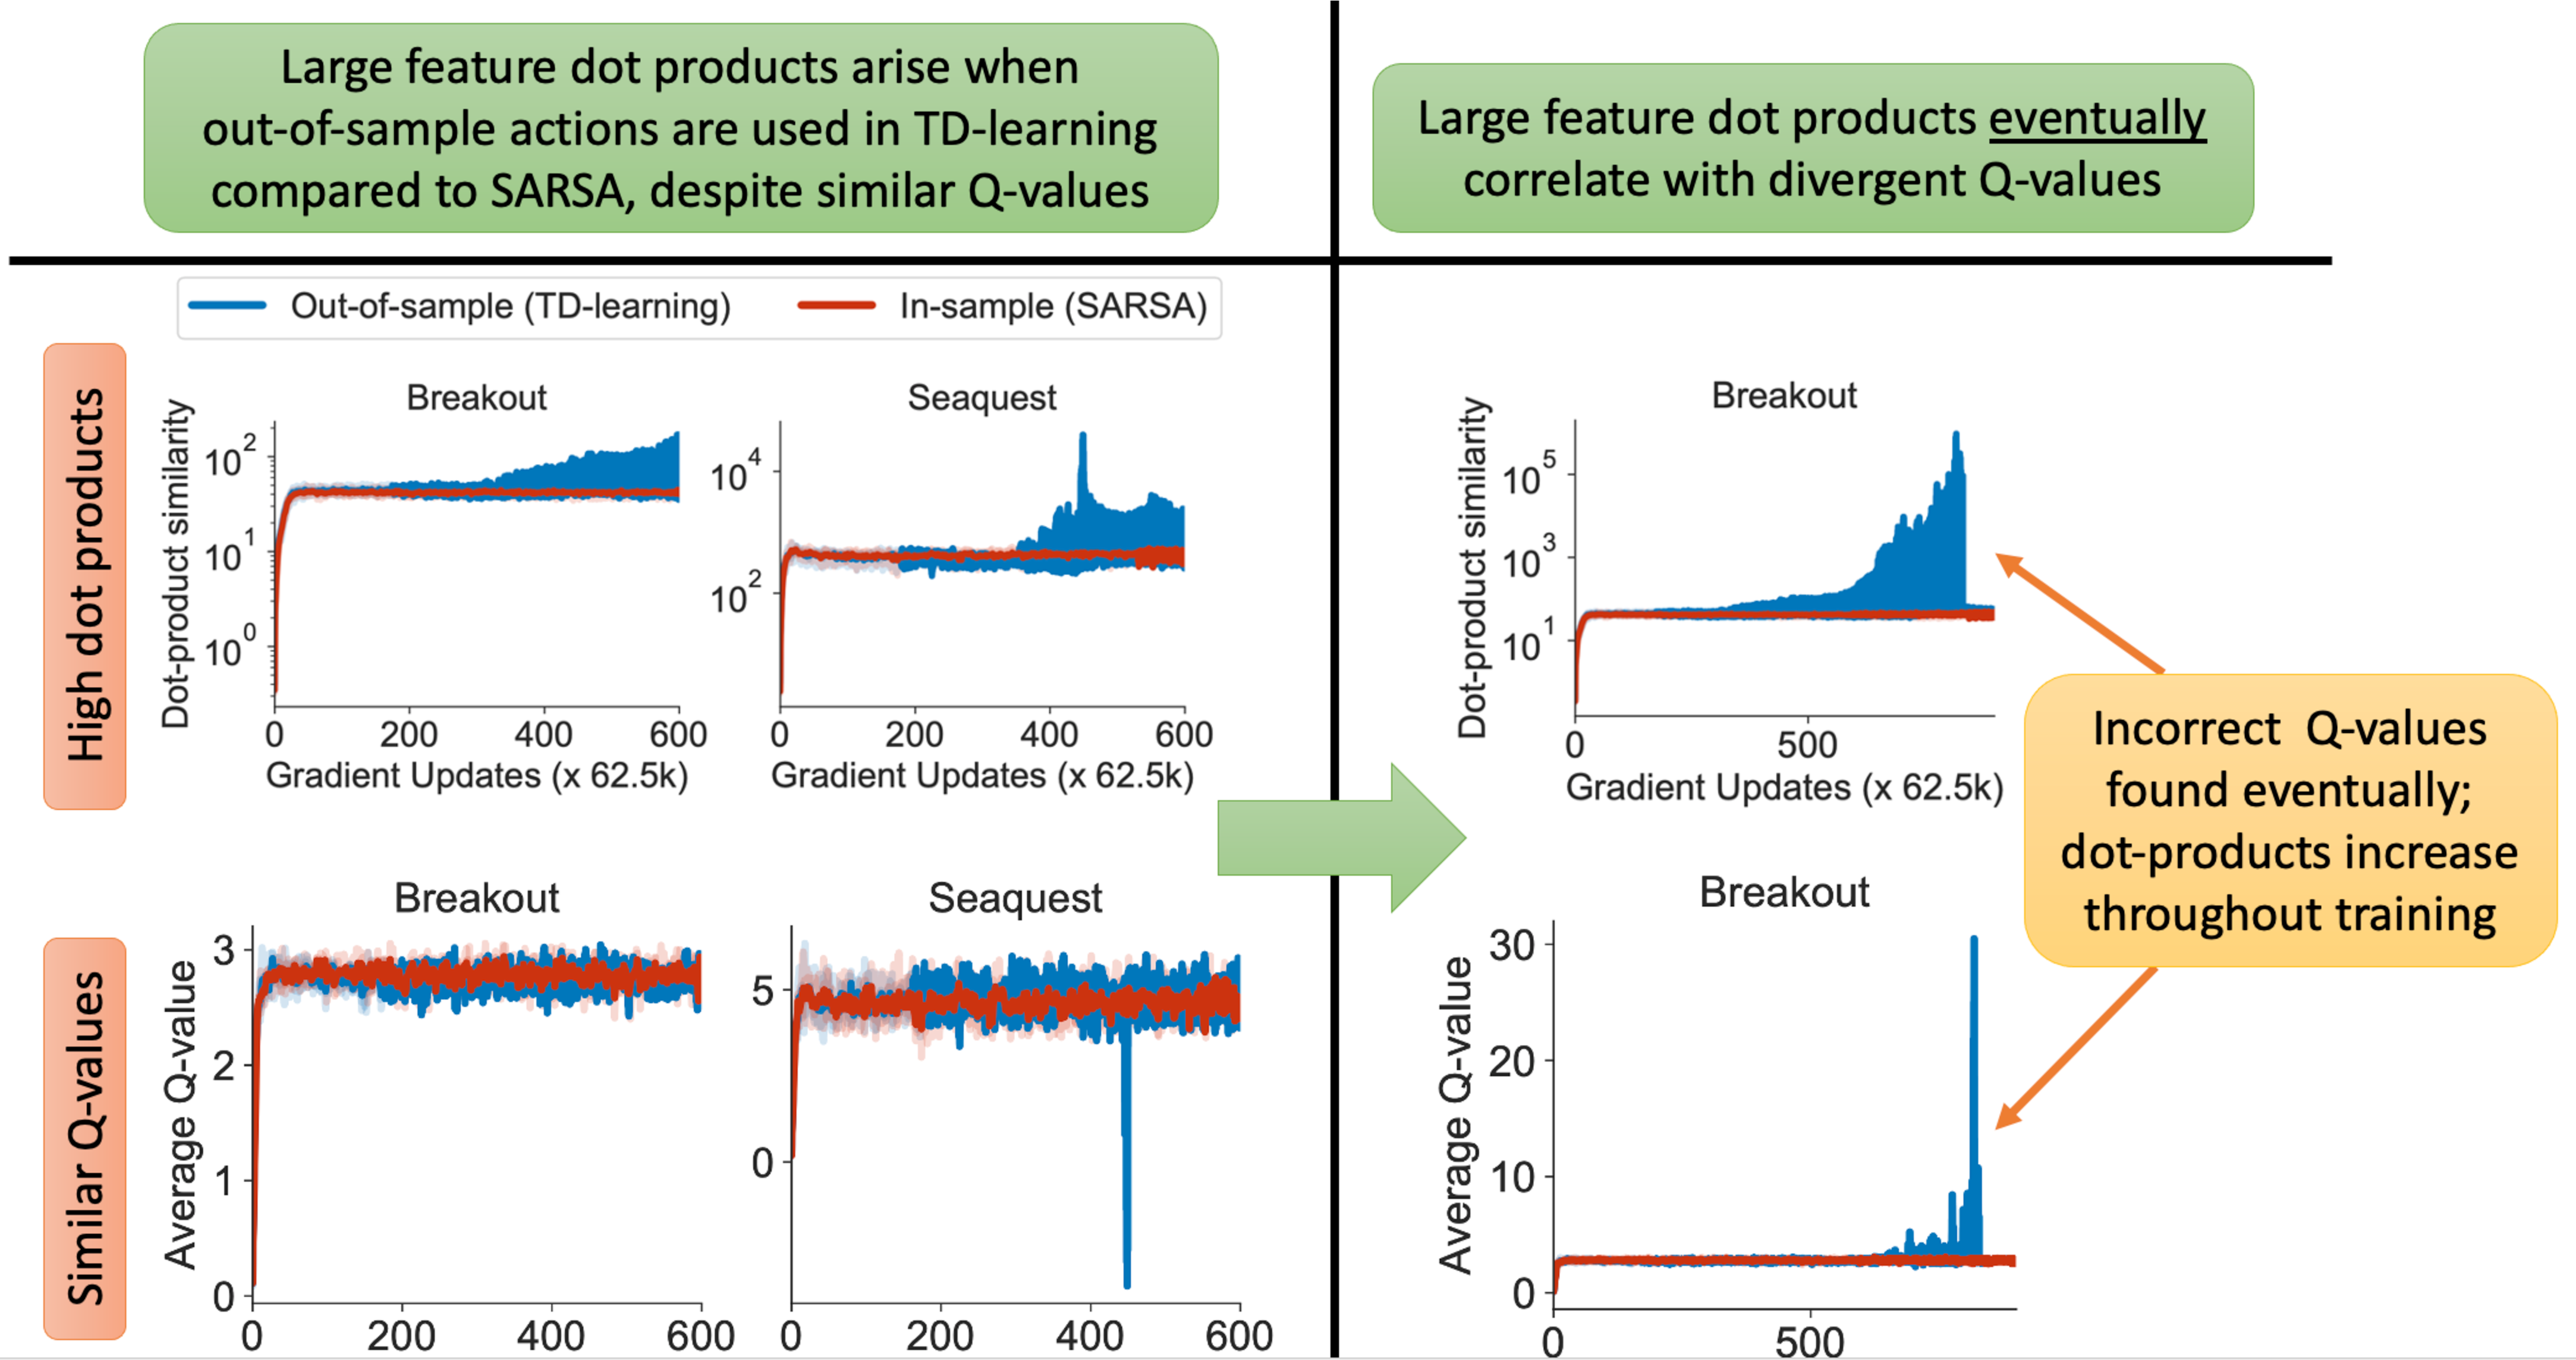
\includegraphics[width=0.67\linewidth]{figures_iclr/final_plot.pdf}~\vline~\vline~
    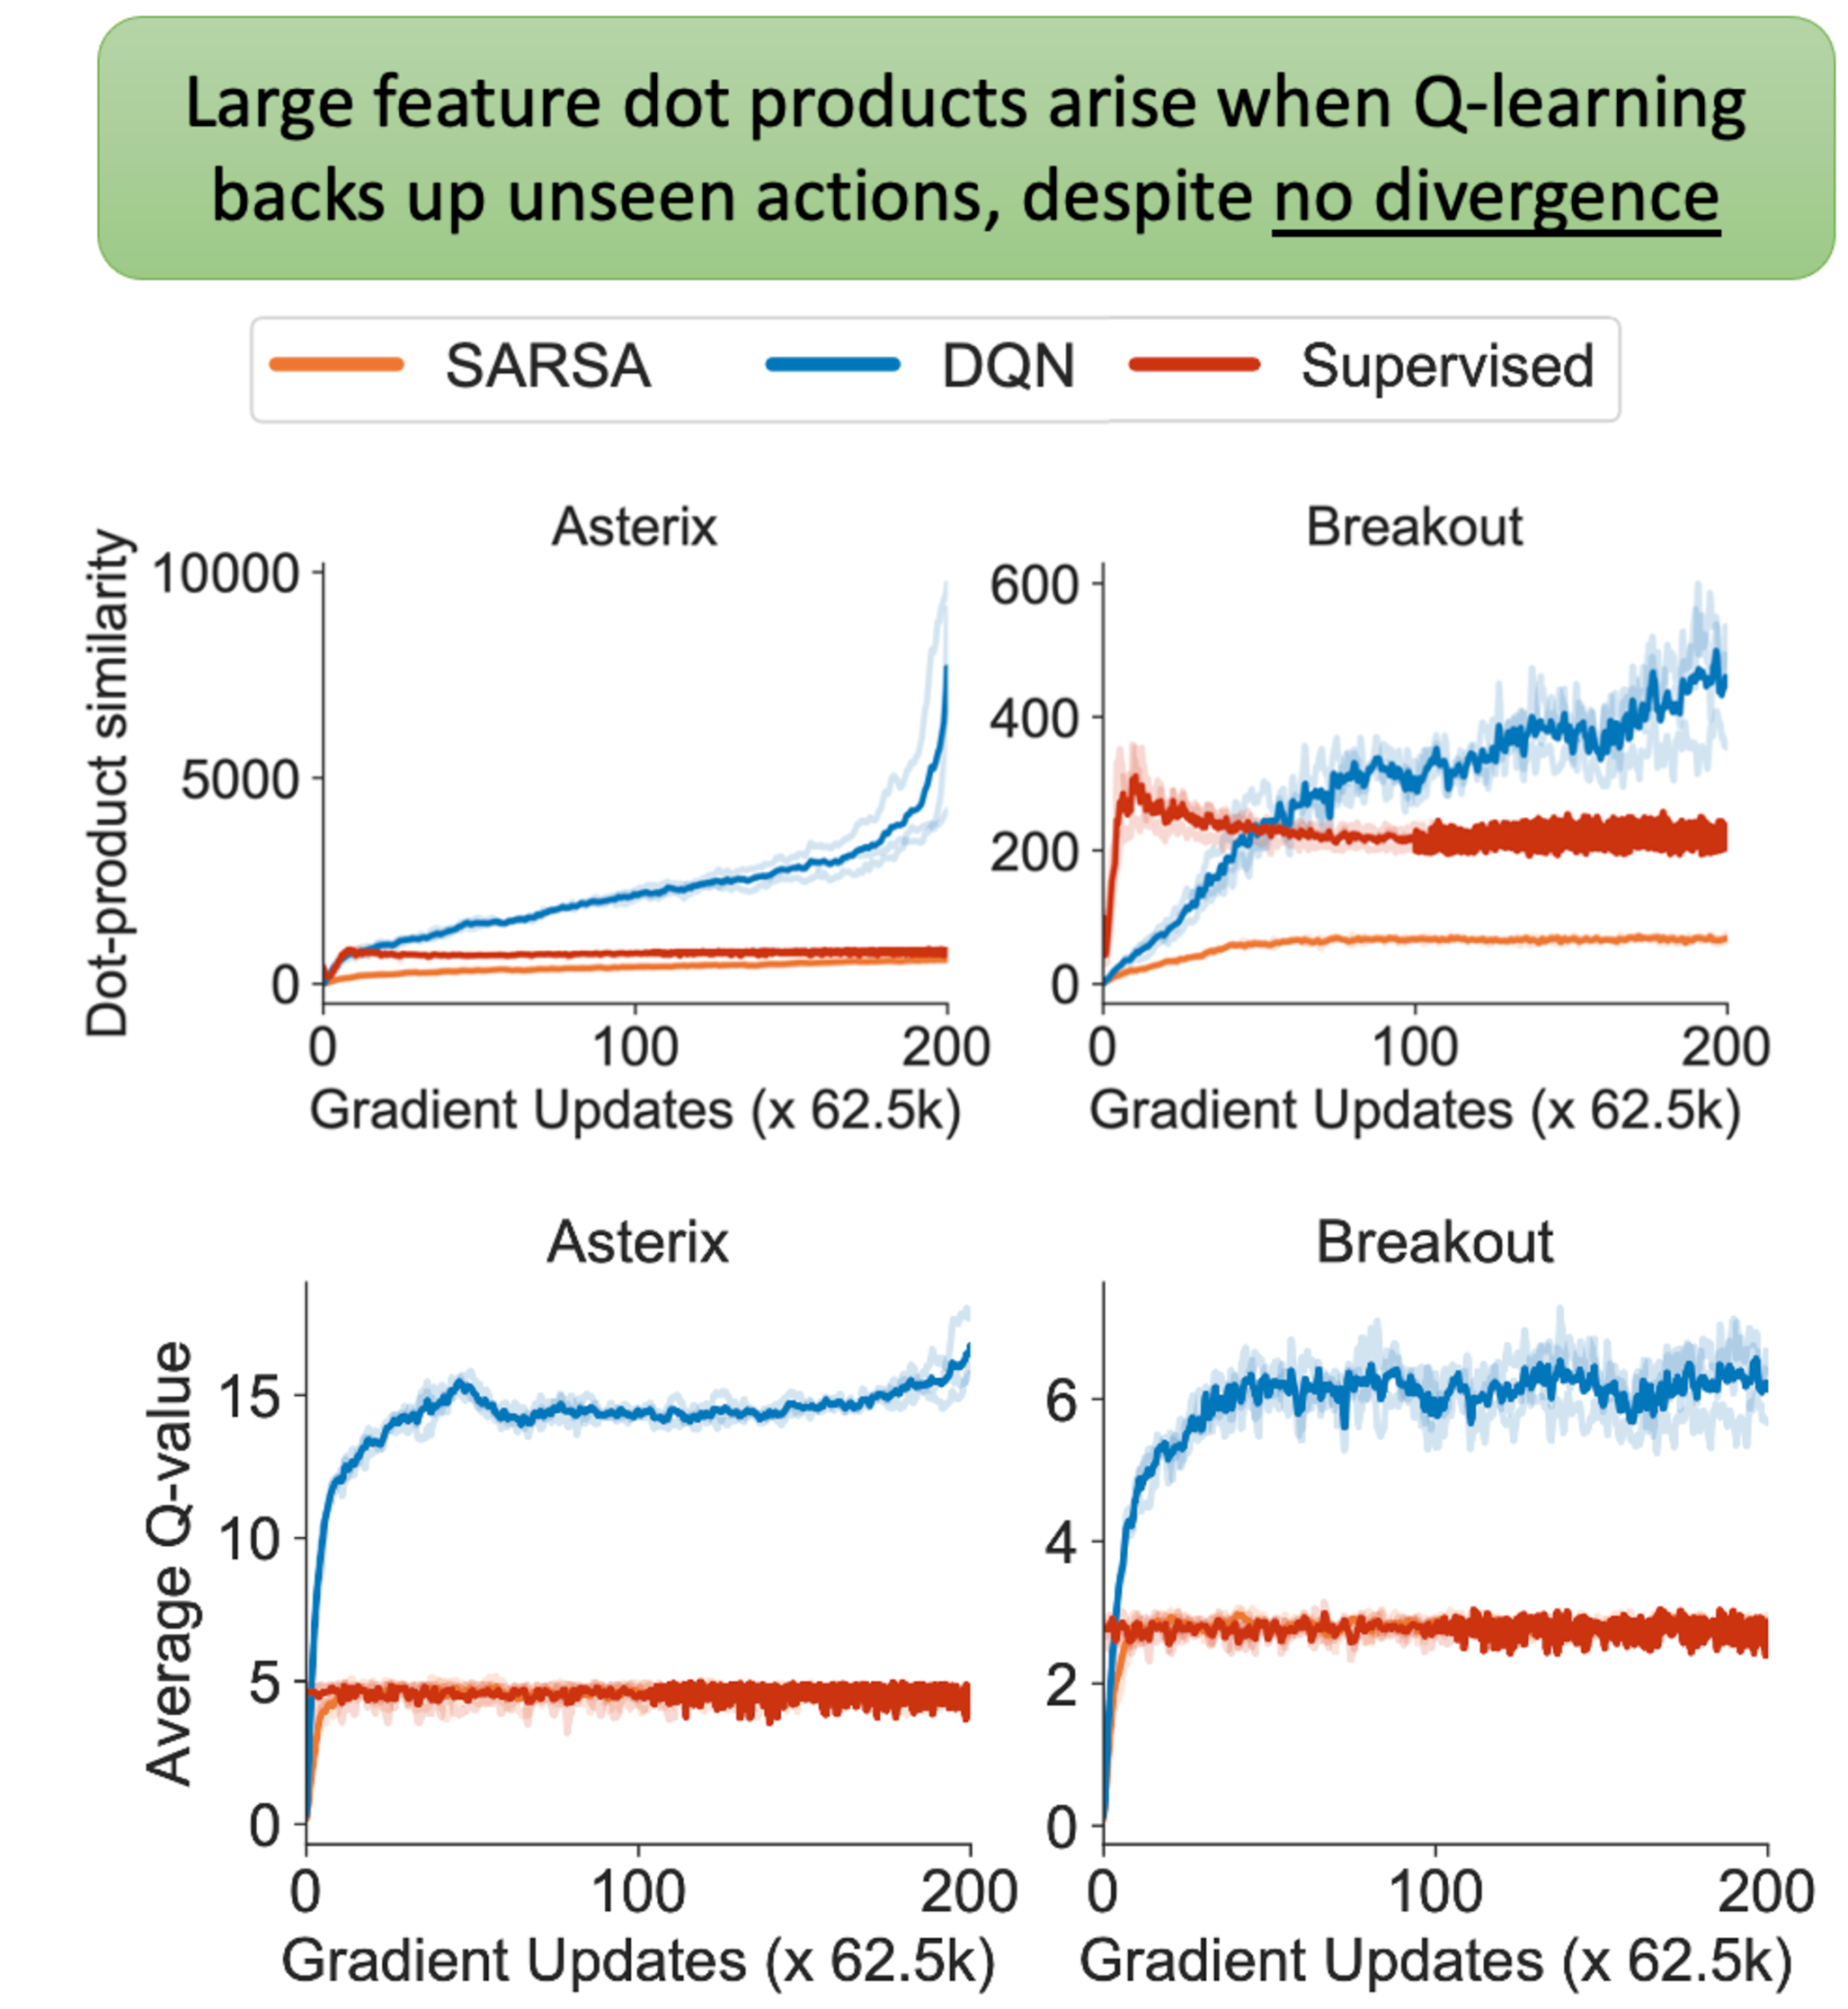
\includegraphics[width=0.32\linewidth]{figures_iclr/final_dqn_fig.pdf}
    \vspace{-0.3cm}
    \caption{\small{Feature dot-products $\phi(\bs, \ba)^\top \phi(\bs', \ba')$ increase during training when backing up from \emph{out-of-sample} but in-distribution actions (\textbf{TD-learning}: left, \textbf{Q-learning}: right), though the average Q-value converges and stays relatively constant. Using only seen state-action pairs for backups (\textbf{offline SARSA}) or not performing Bellman backups (i.e., \textbf{supervised regression}) avoids this issue, with stable and relatively low dot products. \textit{Left}: TD-learning with high feature dot products eventually destabilizes and produces incorrect Q-values, \textit{Right}: DQN attains extremely large feature dot products, despite a relatively stable trend in Q-values.}}  
    \label{fig:dot_products}
    \vspace{-0.6cm}
\end{figure}

\vspace{-5pt}
\subsection{Feature Co-Adaptation And How It Relates To Implicit Regularization}
\label{app:problem_more}
\vspace{-5pt}
In this section, we empirically identify a \emph{feature co-adaptation} phenomenon that appears when training value functions via bootstrapping, where the feature representations of consecutive state-action pairs exhibit a large value of the dot product $\phi(\bs, \ba)^\top \phi(\bs', \ba')$. Note that feature co-adaptation may arise because of high cosine similarity or because of high feature norms. Feature co-adaptation appears even when there is no explicit objective to increase feature similarity.

\textbf{Experimental setup.} We ran supervised regression and three variants of approximate dynamic programming (ADP)
on an offline dataset consisting of 1\% of uniformly-sampled data from the replay buffer of DQN on two Atari games, previously used in \citet{agarwal2019optimistic}. First, for comparison, we trained a Q-function via \textbf{supervised regression} to Monte-Carlo~(MC) return estimates on the offline dataset to estimate the value of the behavior policy. Then, we trained variants of ADP which differ in the selection procedure for the action $\ba'$ that appears in the target value in $\mathcal{L}_\mathrm{TD}(\theta)$ (Equation~\ref{eqn:td_error}). The \textbf{offline SARSA} variant aims to estimate the value of the behavior policy, $Q^{\pi_\beta}$, and sets $\ba'$ to the actual action observed at the next time step in the dataset, such that $(\bs', \ba') \in \mathcal{D}$. The \textbf{TD-learning} variant also aims to estimate the value of the behavior policy, but utilizes the expectation of the target Q-value over actions $\ba'$ sampled from the behavior policy $\pi_\beta$, $\ba' \sim \pi_\beta(\cdot|\bs')$. We do not have access to the functional form of $\pi_\beta$ for the experiment shown in Figure~\ref{fig:dot_products} since the dataset corresponds to the behavior policy induced by the replay buffer of an online DQN, so we train a model for this policy using supervised learning. However, we see similar results comparing \textbf{offline SARSA} and \textbf{TD-learning} on a gridworld domain where we can access the exact functional form of the behavior policy in Appendix~\ref{app:exact_behavior_policy}. %Unlike SARSA, this action $\ba'$ may be different from the one in $\mathcal{D}$, though it comes from the same distribution.
All of the methods so far estimate $Q^{\pi_\beta}$ using different target value estimators.
We also train \textbf{Q-learning}, which chooses the action $\ba'$ to maximize the learned Q-function. While Q-learning learns a different Q-function, we can still compare the relative stability of these methods to gain intuition about the learning dynamics. %To measure feature co-adaptation, we track the average dot product between the learned features at consecutive state-action tuples, $\text{sim}(\bs, \ba, \bs', \ba') := \phi(\bs, \ba)^\top \phi(\bs', \ba')$. 
In addition to feature dot products $\phi(\bs, \ba)^\top \phi(\bs', \ba')$, we also track the average prediction of the Q-network over the dataset to measure whether the predictions diverge or are stable in expectation.

%%AK: also need to figure out an arrangement for figures in the paper
\textbf{Observing feature co-adaptation empirically.} As shown in Figure~\ref{fig:dot_products} (right), the average dot product (top row) between features at consecutive state-action tuples continuously increases for both Q-learning and TD-learning (after enough gradient steps), whereas it flatlines and converges to a small value for supervised regression. We might at first think that this is simply a case of Q-learning failing to converge. However, the bottom row shows that the average Q-values do in fact converge to a stable value. Despite this, the optimizer drives the network towards higher feature dot products. There is no explicit term in the TD error objective that encourages this behavior, 
% and in fact the TD error relatively stays flat \textcolor{red}{(Figure ??)} during training, 
indicating the presence of some implicit regularization phenomenon. This \emph{implicit} preference towards maximizing the dot products of features at consecutive state-action tuples is what we call ``feature co-adaptation.''

\textbf{When does feature co-adaptation emerge?} Observe in Figure~\ref{fig:dot_products} (right) that the feature dot products for offline SARSA converge quickly and are relatively flat, similarly to supervised regression. This indicates that utilizing a bootstrapped update alone is not responsible for the increasing dot-products and instability, because while offline SARSA uses backups, it behaves similarly to supervised MC regression. Unlike offline SARSA, feature co-adaptation emerges for TD-learning, which is surprising as TD-learning also aims to estimate the value of the behavior policy, and hence should match offline SARSA in expectation. The key difference is that while offline SARSA always utilizes actions $\ba'$ observed in the training dataset for the backup, TD-learning may utilize potentially unseen actions $\ba'$ in the backup, even though these actions $\ba' \sim \pi_\beta(\cdot|\bs')$ are \emph{within} the distribution of the data-generating policy. This suggests that utilizing \textbf{out-of-sample} actions in the Bellman backup, even when they are not out-of-distribution, critically alters the learning dynamics. This is distinct from the more common observation in offline RL, which attributes training challenges to out-of-distribution actions~\citep{levine2020offline}, but not out-of-sample actions. The theoretical model developed in Section~\ref{sec:theory} will provide an explanation for this observation with a discussion about how feature co-adaption caused due to out-of-sample actions can be detrimental in offline RL. 

% While action $\ba'$ can be out-of-distribution in the case of Q-learning, this action is sampled from the data-generating distribution of the behavior policy for TD-learning and is hence, not out-of-distribution in this case.

%%AK: does it feel like a jump here, or is it fine?
% The only difference between offline SARSA and Q-learning is whether unseen actions are used to compute the Bellman target\gjt{I don't think that is an accurate statement. The action selection mechanism is different.}:
%%SL.9.17: Yeah, this is correct. Maybe it would be better to mention the TD thing as well in the first paragraph, rather than introducing it for the first time in this paragraph below? That would avoid one very likely criticism you would otherwise get about the comparison between SARSA and Q-learning being non-sensical because they are just learning totally different things
% while $(\bs', \ba')$ used in Q-learning may be unobserved in $\mathcal{D}$, the $(\bs', \ba')$ tuples used in SARSA appear in the dataset, i.e., $(\bs', \ba') \in \mathcal{D}$÷.
%%SL.9.17: some readers won't understand why
% Thus, we might wonder if the use of OOD actions in the backup is the primary culprit for the difference in the observed trends. 

% To understand if this is the case, in Figure~\ref{fig:dot_products} (left), we compare offline SARSA to another variant that we call \textbf{TD-learning},
% %%AK: need to rename TD-learning to something else?
% which utilizes potentially unseen but in-distribution actions sampled from the behavior policy for the Bellman update, such that $\ba' \sim \pi_\beta(\cdot|\bs')$. Like offline SARSA, TD-learning also aims to estimate the value of the behavior policy $Q^{\pi_\beta}$, but it differs from offline SARSA in that the actions $\ba'$ are sampled from the data-generating distribution of the behavior policy. Thus, while they are not \emph{out-of-distribution}, they are also generally not actions that were seen in the dataset $\mathcal{D}$, in contrast to offline SARSA.
% %%SL.9.17: This paragraph is already really hard to read, adding a footnote that creates another branch point for the reader creates an overwhelming cognitive load. Try to merge this footnote into the paragraph, and generally just shorter, more concise, and more digestible sentences.
% % to compute the value of the behavior policy $Q^{\pi_\beta}$. \textbf{Offline SARSA} and \textbf{TD-learning} should match in expectation. 
% As expected, we observe in Figure~\ref{fig:dot_products} (left) that the Q-values predicted by TD-learning match those learned by \textbf{offline SARSA}. However, in contrast to \textbf{offline SARSA}, we find that the dot product similarity for TD-learning increases after enough gradient steps, and this is accompanied by instability in the Q-values. This trend is absent in offline SARSA. This suggests that utilizing out-of-sample actions (even when they are not OOD) in the Bellman backup critically alters the learning dynamics. The theoretical model developed in Section~\ref{sec:theory} provides an explanation for this observation. 
%%AK: one concern: we overload "TD-learning" to mean generic bootstrapping algorithms as well as the "TD learning" baseline we plot. Should we change one of them to something else? Like calling TD-learning generically as bootstrapping and TD learning baseline as FQE.

%%SL.9.17: You can probably shorten this paragraph if you want to save some space
 
% What is the implicit mechanism causing co-adaptation, and why does it occur only when using out-of-sample state-action tuples for the backup? This issue is not corrected by existing offline RL methods, which only avoid out-of-distribution actions~\citep{levine2020offline}, so how does co-adaptation affect offline RL performance? In the next section, we will show how an implicit regularization effect that is studied as a potential benefit of SGD in supervised deep learning can explain this phenomenon, and how this leads to a number of issues in the RL setting.

% \textbf{How do Bellman backups with out-of-sample actions behave?} 
% As shown in Figure~\ref{fig:dot_products} (left), with \textbf{TD-learning}, the dot products steadily increase during training though the average Q-value predictions are roughly constant over the this phase. These Q-values on average match those learned by \textbf{offline SARSA} and \textbf{supervised regression},
% %%SL.7.13: Supervised regression doesn't appear in the left plots!
% but the dot products for \textbf{SARSA} and supervised learning remain flat. In contrast, with \textbf{TD-learning}, the dot products increase after too many gradient steps, and this is accompanied by instability in the Q-values, which then diverge. Note that the only difference between \textbf{TD-learning} and \textbf{SARSA} is the resampling of the target value action, where \textbf{TD-learning} uses a new (out-of-sample) action from the same distribution, while \textbf{SARSA} uses the dataset action.
% %these two approaches quickly converge over the course of training unlike \textbf{TD-learning}. With more training, we find that \textbf{TD-learning} exhibits unstable Q-values, which eventually diverge, whereas the predictions for both \textbf{offline SARSA} and \textbf{supervised regression} converge and do not destabilize with more training.
% % Notably, with \textbf{TD-learning}, the dot-products steadily increase during training and the Q-values eventually diverge, whereas both the dot-products and Q-values of \textbf{offline SARSA} and \textbf{supervised regression} quickly converge and remain stable throughout training (Figure 2). 
% These observations indicate that Bellman backups alone are not responsible for the increasing dot-products and instability because \textbf{offline SARSA} uses Bellman backups, but behaves similarly to \textbf{supervised regression}.
% %%SL.7.13: Again, this is not apparent from the figure, because supervised regression is not shown on the left side!
% On the other hand, \textbf{TD-learning}, which uses out-of-sample actions in the Bellman backup, exhibits increasing dot-products, which eventually ends in  instability, suggesting that out-of-sample actions critically alter the learning dynamics. The theoretical model developed in Section~\ref{sec:theory} provides an explanation for this observation.

% Next, we train two methods that estimate the value of the behavior policy that generated the dataset via dynamic programming. The first approach, which we refer to as  standard \textbf{TD-learning}, estimates $Q^{\pi_\beta}$ by minimizing TD-error $\mathcal{L}_\mathrm{TD}(\theta)$ (Equation in Section~\ref{sec:background}), 
% % $\sum_{\bs, \ba, \bs' \in \mathcal{D}, \ba' \sim {\pi}_\beta(\cdot | \bs')} \left(R(\bs, \ba) + \gamma \bar{Q}_\theta(\bs', \ba') - Q_\theta(\bs, \ba) \right)^2$, 
% where the action $\ba' \sim {\pi}_\beta(\cdot|\bs)$ is sampled from the behavior policy and can be \textit{out-of-sample} for the training dataset, i.e., $(\bs', \ba') \notin \mathcal{D}$, but is \emph{in-distribution}. \aviral{This version is implemented by first learning a model of the behavior policy using supervised classification.} The second approach, which we refer to as \textbf{offline SARSA}, performs Bellman backups from the exact $(\bs', \ba')$ tuple observed in the dataset $\mathcal{D}$ (i.e., $\ba'$ appearing in $\mathcal{L}_\mathrm{TD}(\theta)$ is observed in $\mathcal{D}$).
% % minimizing $\sum_{\bs, \ba, \bs', \ba' \in \mathcal{D}} \left(R(\bs, \ba) + \gamma \bar{Q}_\theta(\bs', \ba') - Q_\theta(\bs, \ba) \right)^2$). 
% Offline SARSA is the same as TD-learning in expectation. However, TD-learning uses potentially out-of-sample actions\footnote{Note that these actions are sampled from the data generating distribution, hence are not out-of-distribution, but may be absent from the training dataset.} in the backup.   As we will show, utilizing out-of-sample state-action tuples in the backup plays a critical role in the learning dynamics.
% Finally, we also train standard \textbf{Q-learning}, which chooses actions $\ba'$ that maximize the learned Q-function. Such actions are also out-of-sample.  


%%SL.7.13: My high-level comment on this section is the following: Right now, your analysis launches into the out-of-sample action discussion right away, without adequately explaining feature co-adaptation. This feels like it's putting the cart before the horse -- before the reader has fully appreciated or even understood what co-adaptation means, they are confronted with this somewhat nuanced discussion about out-of-sample actions. Maybe we should have a couple of sentences before this that basically say "notice how the feature dot products tend to go up right around the same time that things get unstable, isn't that funny? this is what we call feature co-adaptation, let's see what kinds of methods have this issue, and what kinds don't" -- this could be written in just a few sentences, and it should come *before* the discussion of out-of-sample actions, which is secondary to this.


% \begin{figure}[t]
%     \centering
%     \vspace{-5pt}
%     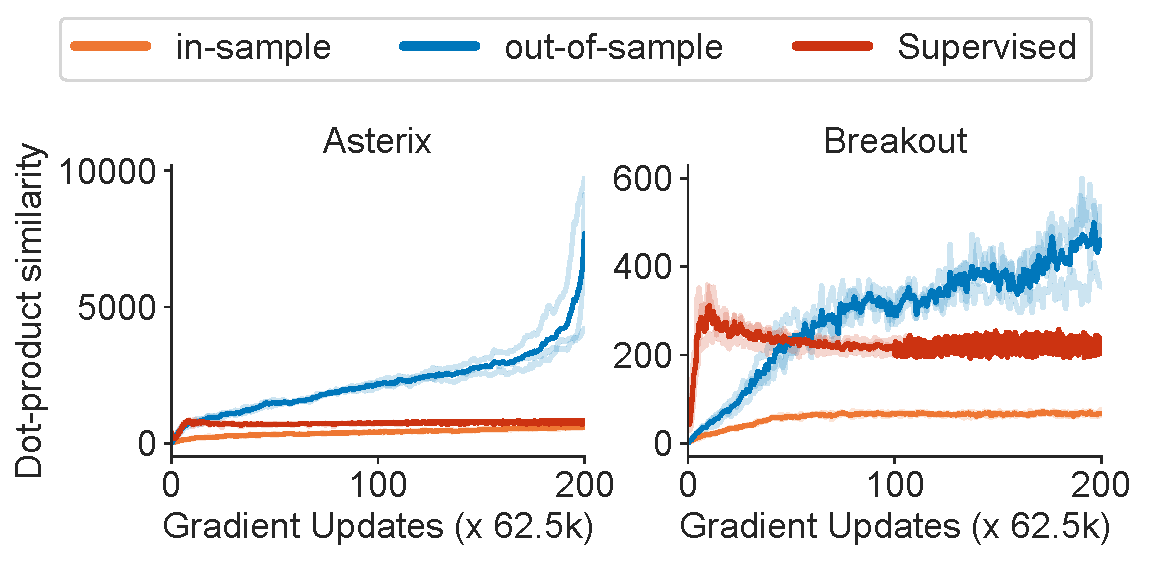
\includegraphics[width=0.45\linewidth]{figures/figure1_dotproduct_dot_products_final.pdf}\\
%     ~~~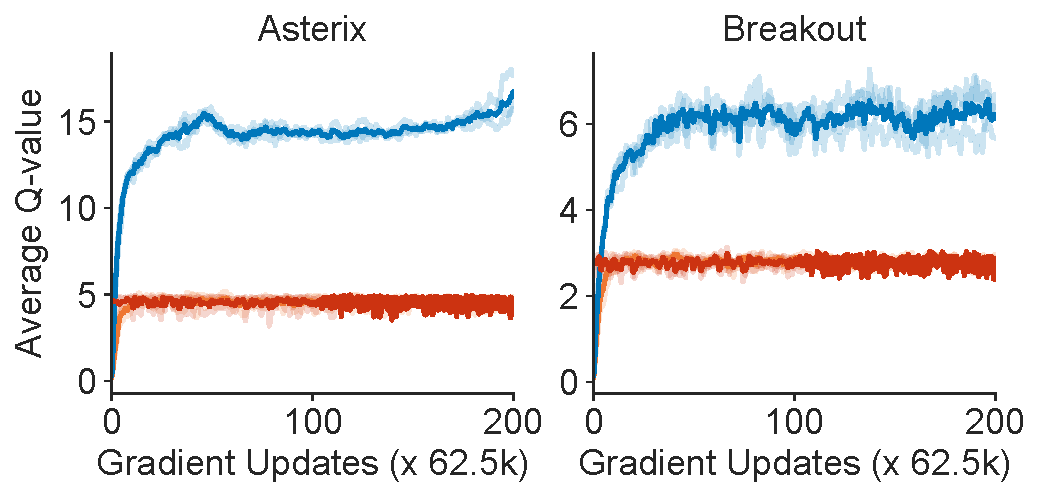
\includegraphics[width=0.45\linewidth]{section3_figs/figure1_dotproduct_q_values (1).pdf}
%     \vspace{-0.24cm}
%     %%SL.5.22: Let's not label it "MC", that's not very informative. Call it "supervised" instead.
%     %%AK: TODO for me, will change it. 
%     %%AK: change labels here
%     \caption{\small{Dot-product $\text{sim}(\bs, \ba, \bs', \ba')$ increases through training when backing up from out-of-sample actions though the average Q-value stays relatively constant, whereas utilizing seen state-action pairs for backups or supervised learning exhibit near-constant dot product similarities as well.}}  
%     \label{fig:dot_products}
%     \vspace{-0.6cm}
% \end{figure}
% \textbf{How do Bellman backups with out-of-sample actions behave?} 
% As shown in Figure~\ref{fig:dot_products} (left), with \textbf{TD-learning}, the dot products steadily increase during training though the average Q-value predictions are roughly constant over the this phase. These Q-values on average match those learned by \textbf{offline SARSA} and \textbf{supervised regression},
% %%SL.7.13: Supervised regression doesn't appear in the left plots!
% but the dot products for \textbf{SARSA} and supervised learning remain flat. In contrast, with \textbf{TD-learning}, the dot products increase after too many gradient steps, and this is accompanied by instability in the Q-values, which then diverge. Note that the only difference between \textbf{TD-learning} and \textbf{SARSA} is the resampling of the target value action, where \textbf{TD-learning} uses a new (out-of-sample) action from the same distribution, while \textbf{SARSA} uses the dataset action.
% %these two approaches quickly converge over the course of training unlike \textbf{TD-learning}. With more training, we find that \textbf{TD-learning} exhibits unstable Q-values, which eventually diverge, whereas the predictions for both \textbf{offline SARSA} and \textbf{supervised regression} converge and do not destabilize with more training.
% % Notably, with \textbf{TD-learning}, the dot-products steadily increase during training and the Q-values eventually diverge, whereas both the dot-products and Q-values of \textbf{offline SARSA} and \textbf{supervised regression} quickly converge and remain stable throughout training (Figure 2). 
% These observations indicate that Bellman backups alone are not responsible for the increasing dot-products and instability because \textbf{offline SARSA} uses Bellman backups, but behaves similarly to \textbf{supervised regression}.
% %%SL.7.13: Again, this is not apparent from the figure, because supervised regression is not shown on the left side!
% On the other hand, \textbf{TD-learning}, which uses out-of-sample actions in the Bellman backup, exhibits increasing dot-products, which eventually ends in  instability, suggesting that out-of-sample actions critically alter the learning dynamics. The theoretical model developed in Section~\ref{sec:theory} provides an explanation for this observation.

%To discern the differences between TD-learning and supervised learning, we first note in Figure~\ref{fig:dot_products} (right) that both the Q-value predictions and dot-product values quickly stabilize for \textbf{supervised regression} (shown in red). A similar convergent behavior in both dot products and learned Q-values is observed when utilizing in-sample actions in the case of \textbf{offline SARSA}, even though SARSA uses Bellman backups (Figure~\ref{fig:dot_products}, ``in-sample''). Next, we turn to case of \textbf{TD-learning}, which utilizes out-of-sample actions. We would expect TD-learning to converge to the same solution as offline SARSA, and we indeed observe similar Q-values in average (compare red vs blue lines in Figure~\ref{fig:dot_products} (left)), however, crucially the feature dot product values are much larger for TD-learning. In fact, the feature dot products in TD-learning continually increase with more training (Figure~\ref{fig:dot_products}) while it stabilizes for offline SARSA. This indicates that even though the Q-function outputs similar values, performing Bellman backups with out-of-sample actions gives rise to increasing dot-product values. Furthermore, as shown in Figure~\ref{fig:dot_products} (middle), once the values of dot-products are large enough (after more training steps), training further leads to an unstable trend in Q-values.


% \vspace{-5pt}

\vspace{-0.2cm}
\subsection{Theoretically Characterizing Implicit Regularization in TD-Learning}
\label{sec:dr3_theory} 
\vspace{-0.2cm}
Why does feature co-adaptation emerge in TD-learning and what do \emph{out-of-sample} actions have to do with it? To answer this question, we theoretically characterize the implicit regularization effects in TD-learning. We analyze the learning dynamics of TD learning in the overparameterized regime, where there are many different parameter vectors $\theta$ that fully minimize the training set temporal difference error. We base our analysis of TD learning on the analysis of implicit regularization in supervised learning, previously developed by \citet{blanc2020implicit,damian2021label}.

\textbf{Background.} When training an overparameterized $f_\theta(\bx)$ via supervised regression using the squared loss, denoted by $L$, many different values of $\theta$ will satisfy $L(\theta)=0$ on the training set due to overparameterization, but \citet{blanc2020implicit} show that the dynamics of stochastic gradient descent will only find fixed points $\theta^*$ that additionally satisfy a condition which can be expressed as $\nabla_\theta R(\theta^*) = 0$, along certain directions (that we will describe shortly). This function $R(\theta)$ is referred to as the implicit regularizer. The noisy gradient updates analyzed in this model have the form:  
\vspace{-0.05in}
\begin{align}
\label{eq:gradient_update}
    \theta_{k+1} \leftarrow \theta_k - \eta \nabla_\theta L(\theta) + \eta \varepsilon_k, ~~ \varepsilon_k \sim \mathcal{N}(0, M).
\end{align}
\citet{blanc2020implicit} and \citet{damian2021label} show that some common SGD techniques fall into this framework, for example, when the regression targets in supervised learning are corrupted with $\mathcal{N}(0, 1)$ label noise, then the resulting $M = \sum_{i=1}^{|\mathcal{D}|} \nabla_\theta f_\theta(\bx_i) \nabla_\theta f_\theta(\bx_i)^\top$ and the induced implicit regularizer $R$ is given by $R(\theta) = \sum_{i}^{|\mathcal{D}|} ||\nabla_\theta f_\theta(\bx_i)||_2^2$. Any solution $\theta^*$ found by Equation~\ref{eq:gradient_update} must satisfy $\nabla_\theta R(\theta^*) = 0$ along directions $\bv \in \mathbb{R}^{|\theta|}$ which lie in the null space of the Hessian of the loss $\nabla^2_\theta L(\theta^*)$ at $\theta^*$,  $\bv \in \text{Null}(\nabla^2_\theta L(\theta^*))$. The intuition behind the implicit regularization effect is that along such directions in the parameter space, the Hessian is unable to contract $\theta_k$ when running noisy gradient updates (Equation~\ref{eq:gradient_update}). Therefore, the only condition that the noisy gradient updates converge/stabilize at $\theta^*$ is given by the condition that $\nabla R(\theta^*) = 0$. This model corroborates findings~\citep{mulayoff2020unique, damian2021label} about the solutions from SGD, which motivates our use. 

\textbf{Our setup.} Following this framework, we analyze the fixed points of noisy TD-learning. We consider noisy pseudo-gradient (or semi-gradient) TD updates with a general noise covariance $M$:
\vspace{-0.05in}
\begin{align}
    \theta_{k+1} = \theta_k - \eta \underbrace{\left( \sum_i \nabla_\theta Q(\bs_i, \mathbf{a}_i) \left(Q_\theta(\bs_i, \mathbf{a}_i)\!- \!(r_i\!+\!\gamma {Q}_{\theta}(\bs'_i, \mathbf{a}'_i))\right) \right)}_{:= g(\theta)} +\eta \varepsilon_k,  ~~ \varepsilon_k \sim \mathcal{N}(0, M)
\label{eq:td_update}
\end{align}
We use a deterministic policy $\mathbf{a}'_i = \pi(\bs'_i)$ to simplify exposition. Following \citet{damian2021label}, we can set the noise model $M$ as $M = \sum_i \nabla_\theta Q(\bs_i, \mathbf{a}_i) \nabla_\theta Q(\bs_i, \mathbf{a}_i)^\top$, or utilize a different choice of $M$, but we will derive the general form first.  Let $\theta^*$ denote a stationary point of the training TD error, such that the pseudo-gradient
$g(\theta^*) = 0$. Further, we denote the derivative of $g(\theta)$ w.r.t. $\theta$ as the matrix $G(\theta) \in \mathbb{R}^{|\theta| \times |\theta|}$, and refer to it as the \emph{pseudo-Hessian}: although $G(\theta)$ is not actually the second derivative of any well-defined objective, since TD updates are not proper gradient updates, as we will see it will play a similar role to the Hessian in gradient descent. For brevity, define $G = G(\theta^*)$, $g = g(\theta^*)$, $\nabla G = \nabla_\theta G(\theta^*) \in \mathbb{R}^{|\theta| \times |\theta| \times |\theta|}$, and let $\lambda_i(P)$ denote the $i$-th eigenvalue of matrix $P$, when arranged in decreasing order of its (complex) magnitude $|\lambda_i(P)|$ (note that eigenvalues can be complex for non-symmetric matrices that we encounter here). 

\textbf{Assumptions.} To simplify analysis, we assume that matrices $G$ and $M$ (i.e., the noise covariance matrix) span the same $n$-dimensional basis in $d$-dimensional space, where $d$ is the number of parameters and $n$ is the number of datapoints, and $n \ll d$ due to overparameterization. We also require $\theta^*$ to satisfy a technical criterion that requires approximate alignment between the eigenspaces of $G$ and the gradient of the Q-function, without which noisy TD may not be stable at $\theta^*$. We summarize all the assumptions in Appendix~\ref{app:dr3_proofs}, and present the resulting regularizer below. 

\begin{tcolorbox}[colback=blue!6!white,colframe=black,boxsep=0pt,top=-3pt,bottom=2pt]
\vspace{2mm}
\begin{theorem}[Implicit regularizer at TD fixed points]
\label{thm:implicit_noise_reg}
Under the assumptions so far, a fixed point of TD-learning,  $\theta^*$, where $Q_{\theta^*}(\bs_i, \mathbf{a}_i) = r_i + \gamma Q_{\theta^*}(\bs'_i, \mathbf{a}'_i)$ for every $(\bs_i, \mathbf{a}_i, \bs'_i) \in \mathcal{D}$ is stable (atttractive) if: \textbf{(1)} it satisfies $\mathrm{Re}(\lambda_i(G)) \geq 0, \forall i$ and $\mathrm{Re}(\lambda_i(G)) > 0$ if $|\mathrm{Imag}(\lambda_i(G))| > 0$, and \textbf{(2)} along directions $\bv \in \mathbb{R}^{\text{dim}(\theta)}, \bv \in \text{Null}(G)$, $\theta^*$ is the stationary point of the implicit regularizer:
\vspace{-0.2cm}
\begin{align}
\label{eqn:regularizer}
\!\!\!\!R_\mathrm{TD}(\theta)\!\!&=\!\!\underbrace{\eta \sum_{i=1}^{|\mathcal{D}|} \nabla Q_\theta(\bs_i, \mathbf{a}_i)^\top \Sigma^{*}_M \nabla Q_\theta(\bs_i, \mathbf{a}_i)}_{\text{implicit regularizer for noisy GD}}
\!\!\!-\!\!\!\underbrace{\eta \gamma \sum_{i=1}^{|\mathcal{D}|} \mathrm{tr}\left(\left[\left[\nabla Q_\theta(\bs'_i, \mathbf{a}'_i)^\top\right]\right]^\top \Sigma_M^* \nabla Q_\theta(\bs_i, \mathbf{a}_i)  \right)}_{\text{additional term in TD learning}}
%%SL.10.27: would it be better to write the trace term as gradQ^T sigma gradQ (since tr(sigma gradQ gradQ^T) = tr(gradQ^T sigma gradQ))? that might make the similarity (but subtle difference) between the two terms more apparent...
    % R_\mathrm{TD}(\theta) = \sum_{i=1}^{|\mathcal{D}|} \mathrm{trace}\left[ \Sigma^{* \top}_M \nabla_\theta Q_\theta(\bs_i, \mathbf{a}_i) \left( \nabla_\theta Q_\theta(\bs_i, \mathbf{a}_i) - \gamma \texttt{Stop}(\nabla_\theta Q_\theta(\bs'_i, \mathbf{a}'_i)) \right)^\top \right].  
    %%SL.9.29: I think it might be clearer if you write this as a difference of two terms, because then the first term will look like the supervised R(theta), but the second one will look clearly weird. The first term then becomes gradQ^T Sigma^T gradQ (and you don't need trace), which is very intuitive (also, Sigma is symmetric, right? so is the transpose symbol there necessary?). Additionally, consider using a less jarring symbol for Stop, so that the equation is typeset so that it looks more like -grad Q [gradQ^T] or something and the stop part is unobtrusive -- that would make it easier for readers to get intuition for what this equation means. Currently it's extremely hard to understand from looking at it.
\end{align}
% \vspace{-0.1in}
where $(\bs_i, \mathbf{a}_i)$ and $(\bs'_i, \mathbf{a}'_i)$ denote state-action pairs that appear together in a Bellman update, $[[\square]]$ denotes the stop-gradient function, which does not pass partial gradients w.r.t. $\theta$ into $\square$. $\Sigma^*_M$ is the fixed point of the  discrete Lyapunov equation: $$\Sigma^*_M := (I - \eta G) \Sigma^*_M (I - \eta G)^\top + \eta^2 M.$$
\end{theorem}
\vspace{1mm}
\end{tcolorbox}
A proof of Theorem~\ref{thm:implicit_noise_reg} is provided in Appendix~\ref{app:dr3_proofs}. Next, we explain the intuition behind this result and provide a proof sketch. To derive the induced implicit regularizer for a stable fixed point $\theta^*$ of TD error, we study the learning dynamics of noisy TD learning (Equation~\ref{eq:td_update}) initialized at $\theta^*$, and derive conditions under which this noisy update would stay close to $\theta^*$ with multiple updates.  This gives rise to the two conditions shown in Theorem~\ref{thm:implicit_noise_reg} which can be understood as controlling stability in mutually exclusive directions in the parameter space. If condition \textbf{(1)} is not satisfied, then even under-parameterized TD will diverge away from $\theta^*$, since $I - \eta G$ would be a non-contraction as the spectral radius, $\rho(I - \eta G) \geq 1$ in that case. Thus, $\theta_k - \theta^*$ will grow or not decrease in some direction. When \textbf{(1)} is satisfied for all directions in the parameter space, there are still directions where both the real and imaginary parts of the eigenvalue $\lambda_i(G)$ are $0$ due to overparameterization\footnote{To see why this is the case, note that $\text{rank}(G) \leq |\mathcal{D}| \ll \text{dim}(\theta)$, and so some eigenvalues of $G$ are $0$.}. 
In such directions, learning is governed by the projection of the noise under the tensor  $\nabla G$,
%%SL.12.5: Are we making that mistake here again where we call the TD pseudo-gradient a derivative? I would recommend being *very* careful about the term derivative. Basically, don't call something a derivative if it's not really a derivative. You can introduce some term for it like pseudo-gradient, but it's very important to clearly distinguish between things that are actual derivatives or gradients, and the TD update. Try to avoid mixing the terminology, but it's OK to define some shorthand term like pseudo-gradient
%%AK: changed it here
which appears in the Taylor expansion of $\theta_k - \theta^*$ around the point $\theta^*$:
\begin{align}
    \label{eqn:nu_k}
    &\theta_{k+1} = \theta_k - \eta \left(g + G (\theta_k - \theta^*) + \frac{1}{2} \nabla G [\theta_k -\theta^*, \theta_k - \theta^*] \right) + \varepsilon_k, ~~ \varepsilon_k \sim \mathcal{N}(0, M)\\
    \implies &\nu_{k+1} = (I - \eta G )\nu_k  - \frac{\eta}{2} \nabla G [\nu_k, \nu_k] + \varepsilon_k,
    \label{eqn:nu_k_actual}
\end{align}
where we reparameterize in terms of $\nu_k := \theta_k - \theta^*$. The proof shows that $\theta^*$ is stable if it is a stationary point of the implicit regularizer $R_\mathrm{TD}$ (condition \textbf{(2)}), which ensures that total noise (i.e., accumulated $\varepsilon_k$ over iterations $k$) accumulated by $\nabla G$ does not lead to a large deviation in $\nu_k$ in directions where $I - \eta G$ does not contract. 
% The total noise accumulated with such noisy backups (Equation~\ref{eqn:nu_k}) admits the covariance matrix $\Sigma^*_M$, and the derivative of the regularizer $\nabla_\theta R_\mathrm{TD}(\theta)$ at an attractive $\theta^*$ must be zero to prevent any deviation in $\nu_k$ in directions where learning is controlled by \textbf{(2)}.   

% To derive the induced implicit regularizer for a stable fixed point $\theta^*$ of TD error, we study the learning dynamics of noisy TD learning (Equation~\ref{eq:td_update}) initialized at $\theta^*$, and derive conditions under which this noisy update would stay close to $\theta^*$ with multiple updates. In this case, we can utilize Taylor expansion around $\theta^*$ to track the evolution of the difference between $\theta_k$ and $\theta^*$, denoted as $\nu_k = \theta_k - \theta^*$ (roughly; modulo some terms we will discuss in Appendix~\ref{app:proofs}), as shown in Equation~\ref{eqn:nu_k}:
% \begin{align}
%     \label{eqn:nu_k}
%     &\theta_{k+1} = \theta_k - \eta \left(g + G (\theta_k - \theta^*) + \frac{1}{2} \nabla G [\theta_k -\theta^*, \theta_k - \theta^*] \right) + \varepsilon_k, ~~ \varepsilon_k \sim \mathcal{N}(0, M)\\
%     \implies &\nu_{k+1} = (I - \eta G )\nu_k  - \frac{\eta}{2} \nabla G [\nu_k, \nu_k] + \varepsilon_k.
%     \label{eqn:nu_k_actual}
% \end{align}
% Our theoretical result derives the implicit regularizer by characterizing conditions on $\theta^*$ that are necessary for the stability of the learning dynamics in Equation~\ref{eqn:nu_k_actual} in the neighborhood around $\theta^*$. 

\textbf{Interpretation of Theorem~\ref{thm:implicit_noise_reg}.} While the choice of the noise model $M$ will change the form of the implicit regularizer, in practice, the form of $M$ is not known as this corresponds to the noise induced via SGD. We can consider choices of $M$ for interpretation, but Theorem~\ref{thm:implicit_noise_reg} is easy to qualitatively interpret for $M$ such that $\Sigma^*_M = I$. In this case, we find that the implicit preference towards local minima of $R_\mathrm{TD}(\theta)$ can explain feature co-adaptation. In this case, the regularizer is simpler:
\begin{align*}
    R_\mathrm{TD}(\theta) := \sum_i ||\nabla Q_\theta(\bs_i, \mathbf{a}_i) ||_2^2 - \gamma \nabla Q_\theta(\bs_i, \mathbf{a}_i)^\top \nabla [[Q_\theta(\bs'_i, \mathbf{a}'_i)]].
\end{align*}
The first term is equal to the squared per-datapoint gradient norm, which is same as the implicit regularizer in supervised learning obtained by \citet{blanc2020implicit,damian2021label} with label noise. However, $R_\mathrm{TD}(\theta)$ additionally includes a second term that is equal to the dot product of the gradient of the Q-function at the current and next states, $\nabla_\theta Q_\theta(\bs_i, \mathbf{a}_i)^\top \nabla_\theta Q_\theta(\bs'_i, \mathbf{a}'_i)$, and thus this term is effectively \emph{maximized}. When restricted to the last-layer parameters of a neural network,
this term is equal to the dot product of the features at consecutive state-action tuples: $\sum_i \nabla_\theta Q_\theta(\bs_i, \mathbf{a}_i)^\top \nabla_\theta Q_\theta (\bs'_i, \mathbf{a}'_i) = \sum_i \phi(\bs_i, \mathbf{a}_i)^\top \phi(\bs'_i, \mathbf{a}'_i)$. The tendency to maximize this quantity to attain a local minimizer of the implicit regularizer corroborates the empirical findings of increased dot product in Section~\ref{app:problem_more}. 

\textbf{Explaining the difference between utilizing seen and unseen actions in the backup.} If all state-action pairs $(\bs'_i, \mathbf{a}'_i)$ appearing on the right-hand-side of the Bellman update also appear in the dataset $\mathcal{D}$, as in the case of offline SARSA (Figure~\ref{fig:dot_products}), the preference to increase dot products will be balanced by the affinity to reduce gradient norm (first term of $R_\mathrm{TD}(\theta)$ when $\Sigma^*_M = I$): for example, for offline SARSA, when $(\bs'_i, \mathbf{a}'_i)$ are permutations of $(\bs_i, \mathbf{a}_i)$, $R_\mathrm{TD}$ is lower bounded by $(1 - \gamma) \sum_i ||\nabla_\theta Q_\theta(\bx_i)||_2^2$ and hence minimizing $R_\mathrm{TD}(\theta)$ would minimize the feature norm instead of maximizing dot products. This also corresponds to the implicit regularizer we would obtain when training Q-functions via supervised learning and hence, our analysis predicts that offline SARSA with in-sample actions (i.e., when $(\bs', \mathbf{a}') \in \mathcal{D}$) would behave similarly to supervised regression. 

However, the regularizer behaves very differently when unseen state-action pairs $(\bs'_i, \mathbf{a}'_i)$ appear only on the right-hand-side of the backup. This happens with any algorithm where $\mathbf{a}'$ is not the dataset action, which is the case for all deep RL algorithms that compute target values by selecting $\mathbf{a}'$ according to the current policy. In this case, we expect the dot product of gradients at $(\bs, \mathbf{a})$ and $(\bs', \mathbf{a}')$ to be large at any attractive fixed point, since this minimizes $R_\mathrm{TD}(\theta)$. This is precisely a form of co-adaptation: \textit{gradients at out-of-sample state-action tuples are highly similar to gradients at observed state-action pairs measured by the dot product}. This observation is also supported by the analysis in Section~\ref{app:problem_more}. Finally, note that the choice of $M$ is a modelling assumption, and to derive our explicit regularizer, later in the paper, we will make a simplifying choice of $M$. However, we also empirically verify that a different choice of $M$, given by label noise, works well.
%%%%%%%%%%%%%%%%%%%%%%%%%%%%%%%%%%%%%%%%%%%%%%%%%%%%%%%%%%


\begin{figure}[t]
    \centering
    % \vspace{-18pt}
    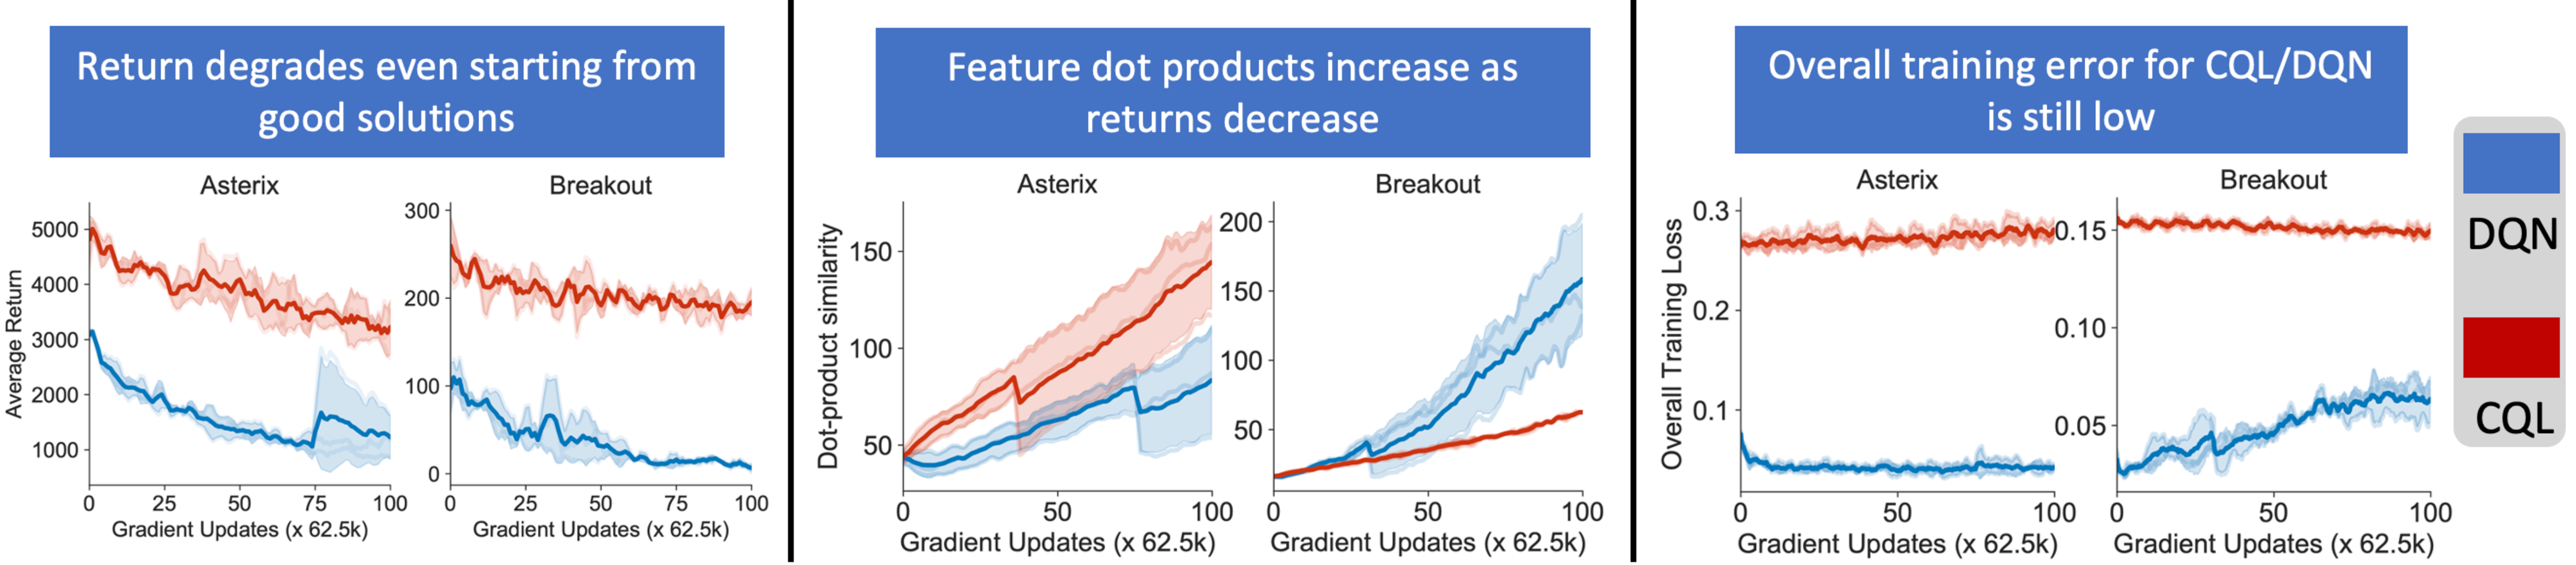
\includegraphics[width=0.99\linewidth]{chapters/dr3/figures_iclr/return_degrades.pdf}
    % 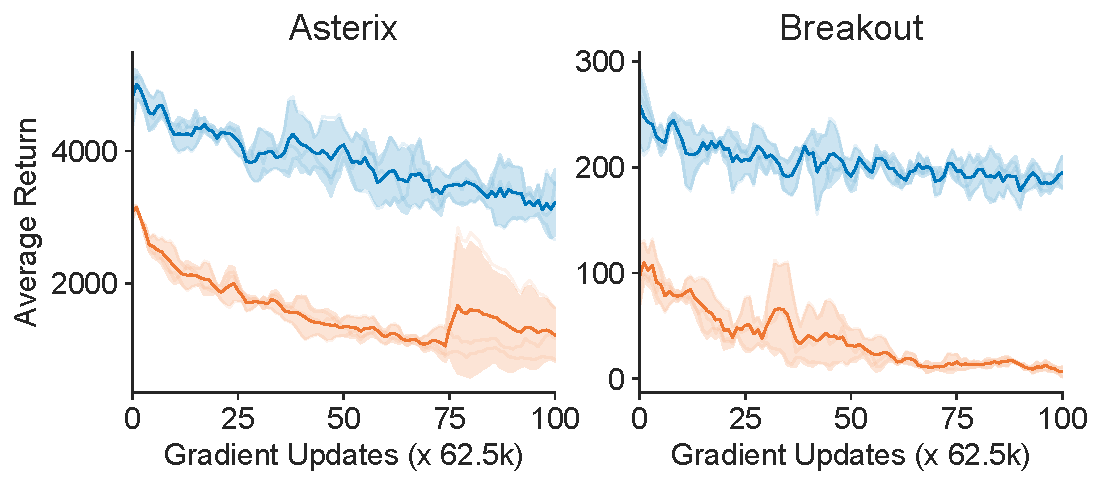
\includegraphics[width=0.49\linewidth]{figures/figure3_neurips_stability_cql_dot_product_both_return.pdf}
    \vspace{-0.3cm}
    \caption{\small{Even when current offline RL algorithms are initialized at a high-performing checkpoint that attains small feature dot products, feature dot products increase with further training and the performance degrades.}}  
    %%SL.7.13: I don't really understand the implication of the last part ("note that the values of the TD error and the overall training loss for either algorithm are generally low and decrease in many cases")
    \label{fig:stability}
    \vspace{-0.3cm}
\end{figure}



\textbf{Why is implicit regularization detrimental to policy performance?}
To answer this question, we present theoretical and empirical evidence that illustrates the adverse effects of this implicit regularizer. Empirically, we ran two algorithms, DQN and CQL, initialized from a high-performing Q-function checkpoint,
%%SL.10.27: This part is going to really throw off some readers. Of course it's not a stable point for TD, because you didn't learn it with TD! Why do we expect the solution found by one method (in this case DR3) to be stable for another method? That doesn't illustrate that TD is bad, just that DR3 changes the fixed point (which it should). But perhaps if you don't want to go into detail about this issue, you could somehow sweep the "obtained using DR3" bit under the rug to avoid distracting the reader?
%%AK: agreed, removed
which attains relatively small feature dot products (i.e., the second term of $R_\mathrm{TD}(\theta)$ is small). Our goal is to see if TD updates starting from such a ``good'' initialization still stay around it or diverge to poorer solutions. Our theoretical analysis in Section~\ref{sec:dr3_theory} would predict that TD learning would destabilize from such a solution, since it would not be a stable fixed point. Indeed, as shown in Figure~\ref{fig:stability}, the policy immediately degrades, and the the dot-product similarities start to increase. This even happens with CQL, which explicitly corrects for distributional shift confounds, implying that the performance drop cannot be directly explained by the typical out-of-distribution action explanations. To investigate the reasons behind this drop, we also measured the training loss function values for these algorithms (i.e., TD error for DQN and TD error + CQL regularizer for CQL) and find in Figure~\ref{fig:stability} that the loss values are generally small for both CQL and DQN. This indicates that the preference to increase dot products is not explained by an inability to minimize TD error. 
%%SL.12.5: I don't understand what "implicit phenomenon" means or how the loss being low indicates this
In Appendix~\ref{app:cql_stability}, we show that this drop in performance when starting from good solutions can be effectively mitigated with our proposed \methodname\ explicit regularizer for both DQN and CQL. Thus we find that not only standard TD learning degrades from a good solution in favor of increasing feature dot products, but keeping small dot products enables these algorithms to remain stable near the good solution.
%%SL.12.5: I slightly tweaked the above sentence, but it can be badly misunderstood as saying that basically our entire evaluation of DR3 has been offloaded into that appendix.

To motivate why co-adapted features can lead to poor performance in TD-learning, we study the convergence of linear TD-learning on co-adapted features. Our theoretical result characterizes a lower bound on the feature dot products in terms of the feature norms for state-action pairs in the dataset $\mathcal{D}$, which if satisfied, will inhibit  convergence: 
\begin{tcolorbox}[colback=blue!6!white,colframe=black,boxsep=0pt,top=-3pt,bottom=2pt]
\vspace{2mm}
\begin{proposition}[TD-learning on co-adapted features]
\label{thm:co_adapted_features_are_bad}
Assume that the features $\Phi = [\phi(\bs, \mathbf{a})]_{\bs, \mathbf{a}}$ are used for linear TD-learning. Then, if 
$$\sum_{\bs, \mathbf{a}, \bs' \in \mathcal{D}} \phi(\bs, \mathbf{a})^\top \phi(\bs', \mathbf{a}') \geq \frac{1}{\gamma} \sum_{\bs, \mathbf{a} \in \mathcal{D}} \phi(\bs, \mathbf{a})^\top \phi(\bs, \mathbf{a}),$$ 
linear TD-learning using features $\Phi$ will not converge. 
\end{proposition}
\end{tcolorbox}
A proof of Proposition~\ref{thm:co_adapted_features_are_bad} is provided in Appendix~\ref{app:new_thm} and it relies on a stability analysis of linear TD. While features change during training for TD-learning with neural networks, and arguably linear TD is a simple model to study consequences of co-adapted features, even in this simple linear setting, Proposition~\ref{thm:co_adapted_features_are_bad} indicates that TD-learning may be non-convergent as a result of co-adaptation.

% \textbf{Comparison to implicit regularization in TD learning with linear function approximation.} Running stochastic gradient descent in overparameterized linear regression finds solutions with the smallest $\ell_2$ norm, which is often regarded as the implicit regularizer. Based on this observation, one might wonder how our derived implicit regularizer relates to minimum norm solutions attained by gradient descent in overparameterized linear TD learning. The implicit regularizer we obtain in  Equation~\ref{eqn:regularizer} would be a constant, independent of the parameter vector $\theta$ for linear TD learning. Thus our regularization specifically captures the effect of SGD on non-linear function approximators, which are absent when studying linear function approximation. 

% \textbf{Takeaways.} We summarize the key takeaways from our theoretical analysis now. \textbf{(1)} \emph{The implicit regularizer at TD fixed points} is shown in Equation~\ref{eqn:regularizer}. The first term corresponds to the regularizer for SGD in supervised learning, while the second term that is unique to TD and leads to an (undesirable) increase in gradient or feature dot products; \textbf{(2)}\emph{Out-of-sample actions exacerbate the implicit regularization effect,} since feature dot products can be easily increased when out-of-sample actions, which do not appear in the dataset, are used to compute Bellman targets; \textbf{(3)} The implicit regularizer in Equation~\ref{eqn:regularizer} is induced via a mechanism unique to non-linear Q-functions, different from overparameterized, linear TD-learning.
% \vspace{-0.15cm}

% \textbf{Theoretically,} we characterize the adverse effects of this implicit regularization by examining the trend in the worst-case error incurred by value-function learning on top of the learned features as feature dot-products increase.

\iffalse
We will first derive the implicit regularization effect induced due to noise in stochastic gradient descent. Following prior work~\citep{blanc2020implicit} in supervised learning, we will model this noise as additive Gaussian noise added to the regression targets. \citet{blanc2020implicit} has identified that in supervised learning, SGD with label noise
%%SL.5.26: is the "label noise" part even significant? almost any supervised learning problem assumes label noise
diverges from a solution $\theta^*$ corresponding to a loss function $L(\theta)$, if and only if it is not a first-order stationary point of:
%%SL.5.26: I found the above sentence pretty hard to parse, can we state this in a simpler way?
\begin{equation*}
    \min_\theta~~ R(\theta) ~~~ \text{s.t.}~~~ L(\theta) = 0,
\end{equation*}
where $R(\theta)$ is an implicit regularizer given by the mean squared L2-norm of the gradient of the learned function with respect to its parameter $\theta$.
%%SL.5.26: add an equation for this
Our goal in this section is to derive the corresponding regularizer for TD-learning, $R_\mathrm{TD}(\theta)$, under similar assumptions, and then analyze its effect on the solution found via TD-learning.  

We first set up the notation. Let $Q_\theta(\bs, \ba)$ denote the Q-network; for brevity, we will use $\bx$ as shorthand for $(\bs, \ba)$, such that $\bx := (\bs, \ba)$ is the input to $Q_\theta$. Given a dataset $\data = \{(\bs_i, \ba_i, r_i, \bs'_i)\}_{[n]}$ and following prior work,
%%SL.5.26: add citation
we will assume that the Q-function minimizes  mean-squared TD-error with added label-noise, $\hat{L}(\theta)$, such that \textcolor{red}{George, can we move the label noise to gradient noise?}
\begin{equation*}
%%SL.5.26: reverse the order here, have \hat{L} come first, then \ell
    \ell_\theta(i) = \frac{1}{2} \left(Q_\theta(\bx_i) - \mathrm{StopGrad}\left[r_i + \gamma Q_\theta(\bx'_i) \right] - \epsilon_i \right)^2; ~~~\epsilon_i \sim \mathcal{N}(0, \sigma^2); ~~~ \hat{L}(\theta) := \frac{1}{n}\sum_{i=1}^n \ell_\theta(i),
\end{equation*}
where $\mathrm{StopGrad}$ denotes the stop-gradient operation typically used in TD-learning, $\epsilon_i$ is random Gaussian scalar noise, and $(\bx_i, \bx'_i)$ represent state-action pairs appearing together in a Bellman backup.
%%SL.5.26: make it more explicit what \bx'_i is
TD-learning would then minimize $\hat{L}(\theta)$ via gradient descent. We will assume that $Q_\theta(\bx_i)$,  $\nabla_\theta Q_\theta(\bx_i)$ and $\nabla^2_\theta Q_\theta(\bx_i)$ are all Lipschitz with some coefficients. 


%%%%%%%%%%%%%%%%%%%%%%%%%% DO NOT DELETE THIS BLOCK %%%%%%%%%%%%%%%%%%%%%%%%%%%%%%%%%%%%%%%%%%%%%%%%%%%
%%%%%%%%%%%%%%%%%%%%%%%%%%%%%%%%%%%%%%%%%%%%%%%%%%%%%%%%%%%%%%%%%%%%%%%%%%%%%%%%%%%%%%%%%%%%%%%%%%%%%%%
% To identify the implicit regularizer, building on \citep{blanc2020implicit}, our strategy would be as follows: Assume that we initialize the parameter $\theta$ to $\theta_0 = \theta^*$. If we can find a regularizer $R_\mathrm{TD}(\theta)$ such that gradient descent on the regularized TD-error loss without label noise, $\bar{L}(\theta) := L(\theta) + \alpha R_\mathrm{TD}(\theta)$ closely follows the trajectory obtained via gradient-descent on TD-error with label noise, $\hat{L}(\theta)$ in a local neighborhood around $\theta^*$, we an utilize the regularized objective $\bar{L}(\theta)$ to reason about trajectories of gradient descent starting the optimal solution $\theta^*$. The gradient-descent update equations for both the objectives are shown below:
% \begin{equation}
% \label{eqn:gradient_descent}
%     \theta_{k+1} \leftarrow \theta_k - \eta \nabla_\theta \hat{L}(\theta_k) ~~~~~~~~~ \bar{\theta}_{k+1} \leftarrow \bar{\theta}_k - \eta \nabla_\theta \left( L(\bar{\theta}_k) + \alpha R_\mathrm{TD}(\bar{\theta}_k) \right).
% \end{equation}
% Simplifying the expression on the left-side we obtain the following:
% \begin{align*}
%     \theta_{k+1} &= \theta_k - \eta \sum_i \nabla_\theta Q_\theta(\bx_i) \left(Q_\theta(\bx_i) - (r_i + \gamma Q_\theta(\bx'_i)) - \epsilon_i \right)\\
%     \implies \theta_{k+1} &= \theta_k - \eta \underbrace{\sum_{i} \nabla_\theta Q_\theta(\bx_i) \left[Q_\theta(\bx_i) - (r_i + \gamma Q_\theta(\bx'_i)) \right]}_{\text{(a)} := \nabla_\theta L(\theta_k)} + \eta  \underbrace{\sum_i \nabla_\theta Q_\theta(\bx_i) \epsilon_i.}_{\text{(b)} \sim \mathcal{N}(0, \sigma^2 \nabla_\theta Q_\theta \nabla_\theta Q_\theta^\top).}
% \end{align*}
% Note that due to the additive nature of label noise, the parameters $\theta_k$ constantly evolve using gradients of the original TD-error loss function without noise (term (a)) along with a data-dependent noise (term (b)) drawn from $\mathcal{N}(0, \sigma^2 \nabla Q_\theta \nabla Q_\theta^\top)$. A natural next step is to obtain the difference of iterates $\theta_k$ and $\bar{\theta}_k$ in a recursive equation:
% \begin{equation}
%     \label{eqn:difference}
%     \nu_{k+1} := \theta_{k+1} - \bar{\theta}_{k+1} \approx \nu_{k} - \eta \nabla^2 L(\theta^*) \nu_k + \varepsilon^*_k, ~~~\text{where}~~ \varepsilon^*_k \sim \mathcal{N}(0, \nabla Q_{\theta^*} \nabla Q_{\theta^*}^\top).   
% \end{equation}
% To obtain Equation~\ref{eqn:difference}, we used another intermediate step of Taylor expansion around the start point $\theta^*$, ignoring terms with two or more powers of $\theta_k - \theta^*$, $\bar{\theta}_k - \theta^*$ as well as two or more powers of learning rate $\eta$. Equation~\ref{eqn:difference} provides a relation on $\nu_k$: $\nu_{k+1} = (I - \eta \nabla^2 L(\theta^*)) \nu_k + \varepsilon_k$,  Additionally, since $\theta^*$ is an optimum, we obtain the following expression for $\nabla^2 L(\theta^*)$:
% \begin{equation}
%     \sum_i \nabla^2 Q_{\theta^*}(\bx_i) \underbrace{\left(Q_{\theta^*}(\bx_i) - (r_i + \gamma Q_{\theta^*}(\bx'_i))\right)}_{=0 \text{~at~} \theta^*} + \sum_i \nabla Q_{\theta^*}(\bx_i) \left(\nabla Q_{\theta^*}(\bx_i) - \gamma \nabla Q_{\theta^*}(\bx'_i)\right)^\top.
% \end{equation}
%%%%%%%%%%%%%%%%%%%%%%%%%%%%%%%%%%%%%%%%%%%%%%%%%%%%%%%%%%%%%%%%%%%%%%%%%%%%%%%%%%%%%%%%%%%%%%%%%%%%%
%%%%%%%%%%%%%%%%%%%%%%%%%%%%%%%%%%%%%%%%%%%%%%%%%%%%%%%%%%%%%%%%%%%%%%%%%%%%%%%%%%%%%%%%%%%%%%%%%%%%%

%%SL.5.26: Can we abstract away some of this derivation into a theorem statement and move the derivation to an appendix? This would help to get the paper under the length limit.
To identify the implicit regularizer, we build on the approach of \citet{blanc2020implicit} for supervised learning. We assume that we initialize the parameter $\theta$ to $\theta_0 = \theta^*$, which is an optimal Q-function, satisfying \emph{all} the Bellman consistency equations on all the states in the MDP, not just the states in the dataset.
%%SL.5.26: Do we need to assume that we *initialize* there? Can we just say that we are analyzing the optimum or something? Is this really the assumption that prior work makes?
Now, we will run gradient descent on the loss $\hat{L}(\theta)$ with a sufficiently small learning rate $\eta$, starting from $\theta_0$. This results in the iterates shown below in Equation~\ref{eqn:gradient_descent}. We will then bound the divergence between the $k$-th gradient iterate $\theta_k$ and $\theta^*$, and derive the condition on $\theta^*$ that allows this divergence $||\theta_k - \theta^*||_2$ to be small. This condition will specify the implicit regularizer $R_\mathrm{TD}(\theta^*)$ at a stable optimum $\theta^*$. The gradient descent equation in Equation~\ref{eqn:gradient_descent} can be simplified as shown below in Equations~\ref{eqn:gradient_descent_simplified} and \ref{eqn:grad_descent2}:
\begin{align}
\label{eqn:gradient_descent}
    \theta_{k+1} &:= \theta_k - \eta \nabla_\theta \hat{L}(\theta_k).\\
    \label{eqn:gradient_descent_simplified}
     \theta_{k+1} &= \theta_k - \eta \sum_i \nabla_\theta Q_\theta(\bx_i) \left(Q_\theta(\bx_i) - (r_i + \gamma Q_\theta(\bx'_i)) - \epsilon_i \right)\\
     \label{eqn:grad_descent2}
    \implies \theta_{k+1} &= \theta_k - \eta \underbrace{\sum_{i} \nabla_\theta Q_\theta(\bx_i) \left[Q_\theta(\bx_i) - (r_i + \gamma Q_\theta(\bx'_i)) \right]}_{\text{(a)} := \nabla_\theta L(\theta_k)} + \eta  \underbrace{\sum_i \nabla_\theta Q_\theta(\bx_i) \epsilon_i.}_{\text{(b)} \sim \mathcal{N}(0, \sigma^2 \nabla_\theta Q_\theta \nabla_\theta Q_\theta^\top).}
\end{align}
Note in Equation~\ref{eqn:grad_descent2} that, due to the additive nature of label noise, the parameters $\theta_k$ evolve based on the gradients of the original TD-error loss function \emph{without} noise ($L(\theta)$, term (a)), along with a data-dependent noise (term (b)) sampled from $\mathcal{N}(0, \sigma^2 \nabla Q_\theta \nabla Q_\theta^\top)$. Next, since $\theta_k$ is initialized in the local neighborhood of $\theta^*$, we can rewrite Equation~\ref{eqn:grad_descent2} in terms of $\nabla^2 L := \nabla^2_\theta L(\theta)|_{\theta^*}$, $\nabla^3 L := \nabla^3_\theta L(\theta)|_{\theta^*}$ and $M := \nabla_\theta Q_\theta \nabla_\theta Q_\theta^\top|_{\theta^*}$ by using Taylor expansion around $\theta^*$. Also note that since $\theta^*$ is a global optimum, $\nabla_\theta L(\theta^*) = 0$. Denoting $\nu_k = \theta_k - \theta^*$, we obtain ($\varepsilon_k \sim \mathcal{N}(0, \sigma^2 \nabla Q_\theta \nabla Q_\theta^\top)$):
%%SL.5.26: why are there two sets of parens on that last equation?
\begin{align}
    \label{eqn:\nu_k}
    \theta_{k+1} ~&= \theta_k - \eta \left( \nabla L + \nabla^2 L (\theta_k - \theta^*) + \frac{1}{2} \nabla^3 L (\theta_k - \theta^*, \theta_k - \theta^*) \right) + \varepsilon_k, ~~~~~~\\
    \label{eqn:recursive_v}
    \implies \nu_{k+1} ~&= (I - \eta \nabla^2 L )\nu_k  - \frac{\eta}{2} \nabla^3 L (\nu_k, \nu_k) + \varepsilon_k, ~~~~ \varepsilon_k \sim \mathcal{N}(0, \eta \sigma^2 M).
\end{align}
From Equation~\ref{eqn:recursive_v} we can make a few observations. First, the distance between $\theta_k$ and $\theta^*$, $||\nu_k||_2$ decreases at a rate proportional to $(I - \eta \nabla^2 L)$. $\nabla^2 L$ only spans certain directions due to the overparameterized nature of the landscape. Thus $\nu_k$ will not contract on along every direction, and the noise $\varepsilon_k$ in each iteration can compound through powers of $(I - \eta \nabla^2 L)$ leading to an increased in the value of $\nu_{k}$,
%%SL.5.26: presumably it makes it increase under some conditions on that matrix?
thus making $\theta_k$ diverge from $\theta^*$. However, if the starting $\theta^*$ is such that the third derivative $\nabla^3 L (\nu_k, \nu_k)$ can compensate for any potential increase in the value of $\nu_k$, then $\nu_{k} \rightarrow 0$ as $k \rightarrow \infty$. Theorem~\ref{thm:implicit_noise_reg} formalizes this to obtain an expression for the resulting implicit regularizer. A proof for Theorem~\ref{thm:implicit_noise_reg} can be found in Appendix ??.
\begin{theorem}[Informal, Implicit regularization at optimal TD-solutions]
\label{thm:implicit_noise_reg}
Assuming notations
%%SL.5.26: "Assuming notations" seems like a weird phrase
and conditions of label-noise gradient descent on TD error discussed so far, a global minimizer of TD error $\theta^*$ on the dataset $\mathcal{D}$ is a stable optimum if and only if it minimizes implicit regularizer $R_\mathrm{TD}(\theta)$ given by:
\begin{equation}
\label{eqn:regularizer}
    R_\mathrm{TD}(\theta) = \mathrm{tr} \left(\sum_{i=1}^n \nabla_\theta Q_\theta(\bx_i) \left( \nabla_\theta Q_\theta(\bx_i) - \gamma \nabla_\theta Q_\theta(\bx'_i) \right)^\top \right).
\end{equation}
\end{theorem}
\textbf{Interpretation of Theorem~\ref{thm:implicit_noise_reg}.} Theorem~\ref{thm:implicit_noise_reg} indicates that out of all possible global minimizers $\theta^*$ of the TD error
%%SL.5.26: this is a fairly basic point, but I think when we introduce the notion of implicit regularization earlier, it might help to expand on what this "out of all possible minimizers" thing means. E.g., something like this: When training overparameterized functions, such as deep networks, multiple different parameter vectors $\theta$ will minimize $L(\theta)$. But not all of these minimizers will generalize equally well. \citet{someone} proposes that the minimizer found via SGD will satisfy the following constrained optimization problem: [stuff], where $R(\theta)$ is an \emph{implicit} regularizer that arises from the structure of SGD with overparameterized models. Intuitively, $R(\theta)$ causes SGD to prefer simpler (and therefore more generalizable) solutions, even when we might otherwise expect overparameterized models to be liable to overfit. This model has been put forward as one explanation for the effective generalization of overparameterized deep networks~\citep{stuff}. [this could go at the top of Sec 3.2.1 for example]
on the training dataset, gradient descent with label noise will only stabilize at a minimizer of $R_\mathrm{TD}(\theta)$. $R_\mathrm{TD}$ consists of two types of terms: positive terms equal to gradient norms, $\sum_i ||\nabla_\theta Q_\theta(\bx_i)||^2_2$, and additional negative terms equal to the expected dot-product of gradients at consecutive states, $\sum_\theta Q_\theta(\bx_i)^\top \nabla_\theta Q_\theta(\bx'_i)$.
%%SL.5.26: Is it completely obvious where these come from? I realize this is just algebra, but we could spoon-feed it to the reader more by writing out the distributed equation so that these terms actually show up.
If all state-action pairs $\bx'_i$ appearing on the right-hand-side of the Bellman update also appear in the dataset $\mathcal{D}$, as in the case of SARSA (Figure~\ref{fig:dot_products}), they would also contribute to the gradient norm term, and the value of $R_\mathrm{TD}$ will be bounded below.  We can show that in this case the optimal $\theta^*$ would effectively minimize $(1 - \gamma) \sum_i ||\nabla_\theta Q_\theta(\bx_i)||_2^2$.
%%SL.5.26: can we make these statements a bit more formal? e.g., have a corollary or something for the special case where all x' are in the dataset, and another one for the case where that is not true?
This corresponds to a regularizer one would obtain when training the Q-network via pure supervised learning~\citep{blanc2020implicit}, indicating that SARSA is regularized in similar ways as supervised regression. 
%%AK: is there consensus on this aspect?

%%AK: I am sure the para below doesnt have a great flow. If someone has any suggestions to make it more dramatic, it will be great -- this is the key RL explanation part of this math.
On the other hand, if a state-action pair $\bx'_i$ only appears on the right-hand-side of the backup, \ie, $(\bs', \ba')$ correspond to out-of-sample state-action pairs,
%%SL.5.26: remind the reader why this would be the case, like this: However, the regularizer behaves very differently when some state-action pairs $\bx'_i$ only appear on the right-hand-side of the backup. This happens with any algorithm where $\ba'$ is not the dataset action, which is the case for all actor-critic and Q-learning algorithms that compute target values by selecting $\ba'$ according to the current policy. Note that $(\bs',\ba')$ does not need to be \emph{out-of-distribution}, merely \emph{out-of-sample}, and hence this would even be the case when evaluating $\pi_\beta(\ba'|\bs')$ with samples from $\pi_\beta(\ba'|\bs')$ for the target value actions.
then the implicit regularizer, $R_\mathrm{TD}(\theta)$ is minimized only at solutions $\theta^*$ for which gradients at $\bx_i$ and the corresponding $\bx'_i$ are very similar in terms of dot-product.
%%SL.5.26: some pretty informal statements here, can we summarize this more precisely in a formal corollary?
This is the co-adaptation phenomenon observed in Section~\ref{sec:analysis}: gradients at out-of-sample state-action pairs $\bx'_i$ are extremely similar to the gradients at $\bx_i$ at the resulting optimum.
%%SL.5.26: gradients are similar? or features are similar?
Section~\ref{sec:analysis} instead demonstrated the co-adaptation phenomenon for penultimate layer features, which are also the gradients with respect to the parameters of the last layer, since these values are cheap to compute.
%%SL.5.26: put the above in a footnote, phrase like this: One discrepancy is that Section~\ref{sec:analysis} analyzes dot products between the last-layer features, whereas this derivation focuses on dot products between gradients. Note, however, that the last-layer features are the gradients of the weights in the last layer. [maybe allude to some NTK stuff?]. Alternatively, given that you use "gradients" and "features" interchangeably below, you could also put some discussion like this in the main text, but earlier: Note that this regularizer concerns the \emph{gradients} of the model. However, regularization of gradients and regularization of features are closely related~\citep{something} -- for example, the gradients of the last-layer weights are equal to the penultimate layer features for networks with linear readout layers.
Thus, we have shown that stochastic gradient descent on the TD-error tends to stabilize only at solutions that exhibit highly co-adapted features between out-of-sample points used for the backup and the points in the dataset. \textcolor{red}{also add when it will diverge; tr(...) cant be < 0, else we wont contract.}
\fi


\iffalse
\subsubsection{Implicit Regularization of Neural Network Architectures}
%%SL.5.26: Change the title -- the point is not that it's architecture specific, but that it is focused on overparameterization and min norm.

In the previous section, we showed, that agnostic of the neural network architecture, implicit regularization arising out of the stochasticity in SGD produces Q-functions with highly co-adapted features. In this section, we analyze a different kind of implicit regularization originating from the inductive bias and invariance of the neural network architecture.
%%SL.5.26: This seems like a really strange way to "sell" this analysis -- it's basically saying that before we analyzed the general case, now we'll make some more (unrealistic) assumptions and show that the results still hold under these additional (unrealistic) assumptions. That's a very strange statement. The fact that this analysis is architecture-specific is not really a plus. Can we come up with a better way to motivate why we have this analysis? A reasonable way to go could be something like: In this section, we will show that a similarly deleterious implicit regularization effect in TD-learning can be derived from a very different model of implicit regularization with overparameterized deep networks, based on minimum norm solutions. [and then at the end of this subsection, you can conclude with something like: We've shown that two very different models of implicit regularization in deep nets proposed in prior work~\citep{} both lead to the same conclusion in the TD-learning setting: the very same implicit regularization effects that promote effective generalization in supervised deep learning lead to learning of features that can fail to distinguish between successive state-action tuples in the TD-learning setting.]
For this analysis, we study a 2-layer wide ReLU network using ideas from prior works~\citep{blanc2020implicit,savarese2019infinite,wei2019regularization}.
%%SL.5.26: can we rephrase the above sentence and talk about how we adopt a similar model of implicit regularization as prior work?
For simplicity, we assume that the input space of the Q-function is 1-dimensional, which can be attained by mapping state-action pairs $(\bs_i, \ba_i)$ to a one-dimensional representation $\bx_i \in \mathbb{R}$, though our argument can potentially be generalized to higher-dimensional inputs analogous to \citet{}.
%%SL.5.26: Whoa, that seems like a crazy assumption. Is that really how prior work does it?? I mean, I can see how this can be made to work, but it's an enormous leap.
%%AK: cite the savarese paper 2 from 2019 that uses radon transform

To begin, we define a canonical 2-layer ReLU network with 1D inputs: $Q_\theta(\bx_i) = \sum_i \bw_i \sigma(\ba_i \bx_i + \bb_i) + \bd_i$, where $\sigma(\cdot) = \max(\cdot, 0)$ is the ReLU function. It is well known~\citep{wei2019regularization,savarese2019infinite} that minimizing $L(\theta) = \sum_i (Q_\theta(\bx_i) - y_i)^2$ for input-output pairs $(\bx_i, y_i)$ on a 2-layer ReLU network of sufficient width produces a solution that satisfies the following optimization (left):
%%AK: The para above is not talking about TD-learning but optimizations already use TD, so I need to fix that.
%%SL.5.26: yeah, this is an issue -- above says y, below says r + gamma*Q
\begin{equation}
\begin{aligned}
    &\text{\textbf{Neural Network parameterization}} \\
    \min_{\bw, \ba, \bb, \bd}~~& ||\bw||_1 \\
    \text{s.t.}~&~ \forall~ \bx_i \in \mathcal{D},~~ Q_\theta(\bx_i) = r_i + \gamma \bar{Q}_\theta(\bx'_i) 
    \label{eqn:relu_nets}
\end{aligned}
\;~~ \vline\;
\begin{aligned}
    &\text{\textbf{Function space parameterization}} \\
    ~~~\min_{Q}~~& \int_{-\infty}^{\infty} |Q''(\bx)| d \bx \\
    \text{s.t.}~~&~ \forall \bx_i \in \mathcal{D}, ~~ Q(\bx_i) = r_i + \gamma \bar{Q}(\bx'_i).
\end{aligned}
\end{equation}
The optimization on the left can be converted to a function space parameterization (Equation~\ref{eqn:relu_nets}, right) that minimizes the second-derivative of the function $Q''(\bx)$ w.r.t. the input $\bx \in \mathbb{R}$ while fitting the data. This amounts to fitting the smoothest possible function that attains zero Bellman error.
%%SL.5.26: Let's just introduced the supervised model *first*, and only then talk about Bellman error, otherwise we are throwing more at the reader than they can reasonably handle.
In supervised learning this gives rise to a piecewise linear function with kinks at the points from the dataset, $\bx_i \in \mathcal{D}$ (Theorem 3.1 in \citet{savarese2019infinite}). In our case, we are interested in answering the following question: Among all solutions with zero Bellman error on the training data, do co-adapted solutions attain maximum smoothness? 
%%SL.5.26: That doesn't seem like the right way to pose the question, because "maximum smoothness" is a vague and imprecise term. Let's rather refer to the formal statement of the objective.

To answer this question, we first set up some notation. Let $(\bx_i, \bx'_i)$ be the representations of state-action tuples that appear together in a Bellman update.
%%SL.5.26: already defined this
Without loss of generality, let $\{\bx_i\}_{[n]} \in \mathcal{D}$ be ordered as $\bx_1 < \bx_2 < \cdots < \bx_N$. We further make a locality assumption on the consecutive tuples:
\begin{assumption}[State-action pairs on two sides of a Bellman backup are close to each other]
\label{assumption:state_next_state_are_close}
If $(\bx_i, \bx'_i)$ appear on the two sides of the Bellman equation, and if $\bx_{i-1}$ and $\bx_{i+1}$ be the left and right neighbors of $\bx_i$ observed in $\mathcal{D}$, then, we assume $|\bx_i - \bx'_i| \leq \min \left(|\bx_i - \bx_{i-1}|, |\bx_{i+1} - \bx_i| \right)$. 
\end{assumption}
Assumption~\ref{assumption:state_next_state_are_close} encodes the notion that the next state,
%%SL.5.26: Don't overload terminology, you're using "state" to mean two different things. This will be perceived as (intentionally) deceptive, because the consecutive actions are *not* similar.
$\bx'_i$, is closer to the current state $\bx_i$ compared to the neighbors of $\bx_i$ found in the dataset. This is reasonable to assume in practice, where states and next states generally do not differ from each other by a huge amount, often changing by a few pixels.
%%SL.5.26: I disagree with the above statement -- why the heck would \bx'_i be closer to \bx_i than \bx_{i+1}? Presumably the next action of pi_beta is at least as close to the current action of pi_beta than the next action of pi. Maybe you mis-stated something above and intended to write something else? But as written this just doesn't seem plausible.
%%AK: is there a better, simpler assumption? And can I cite something to say that the states- next states are closeby?
Under Assumption~\ref{assumption:state_next_state_are_close}, we show the following result:
%%AK: refine theorem statement and verify edge cases once (a lot of the edge cases are measure zero, so maybe just almost surely will eliminate time?)
\begin{theorem}[Informal, ReLU networks attain additional kinks
%%SL.5.26: let's avoid informal statements in theorems ("kinks")
and learn incorrect Q-values]
\label{thm:relu_nets_kinks}
Assuming~\ref{assumption:state_next_state_are_close} and other notation from this section, the optimal solution for Equation~\ref{eqn:relu_nets} (right) consists of kinks
%%SL.5.26: that doesn't seem like a precise theorem statement...
at $\mathcal{D} \cup \{\bx'_1, \cdots, \bx'_n\}$. Moreover, the Q-values at any $\bx_j$ for which $\bx'_j \notin \mathcal{D}$ will be incorrect.
%%AK: TODO: refine the theorem to make it more formal
\end{theorem}
%%AK: TODO; also add SARSA discussion?
When fitting supervised targets to a deep ReLU network, the resulting solution is a piecewise linear function, with pieces intersecting only at the datapoints $\bx_1, \cdots, \bx_n$. On the other hand, Theorem~\ref{thm:relu_nets_kinks} shows that the optimal solution that satisfies Bellman equations will have additional kinks on out-of-sample state-action tuples used for the backup, i.e., $\{\bx'_1, \cdots, \bx'_n\} \backslash \mathcal{D}$. These kinks will alter the values learned at several other state-action pairs, while still satisfying Bellman constraints on the training data and being more smooth as measured by the integral of the second derivative of the function. This is a form of co-adaptation: implicit regularization towards smooth functions in a ReLU network makes predictions at $\bx$ and $\bx'$ coupled together so as to maximize smoothness. Having seen that implicit regularization stemming from a variety of factors including noisy updates and neural network architectures when combined with TD error and gradient descent and its direct relationship with feature co-adaptation, the next section aims to devise an explicit regularizer that can tackle these adverse effects of implicit regularization.   
\fi


\iffalse
\subsection{Consequences of Feature Co-Adaptation in TD-Learning}
Having seen that TD-learning co-adapts features at unseen actions to features at state-action tuples in the dataset, we now study its consequences. We will show that this co-adaptation can prevent learning high-frequency information in the Q-function crucial for control and destabalize learning, even when initialized in the vicinity of a good solution.

\begin{wrapfigure}{r}{0.4\textwidth}
    \centering
    \vspace{-22pt}
    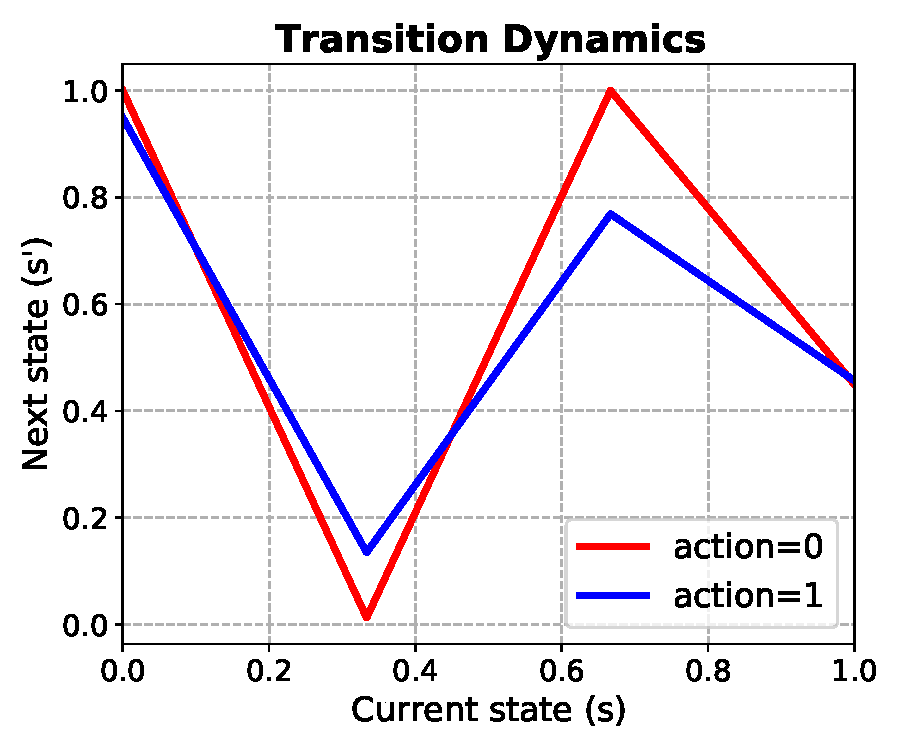
\includegraphics[width=0.48\linewidth]{section3_figs/dynamics.pdf}
    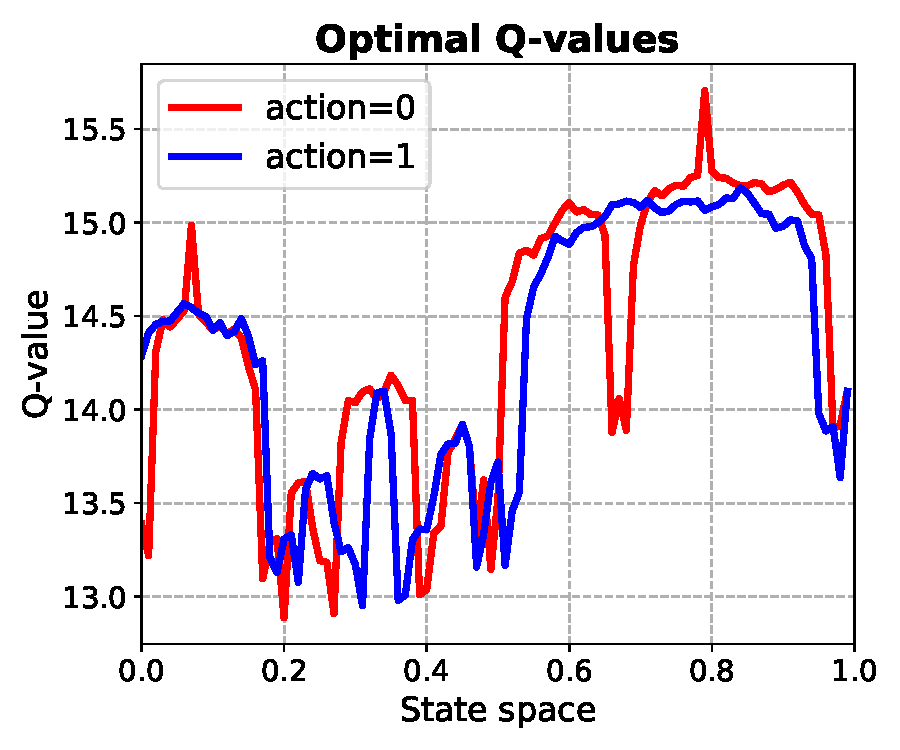
\includegraphics[width=0.48\linewidth]{section3_figs/optimal_q.pdf}
    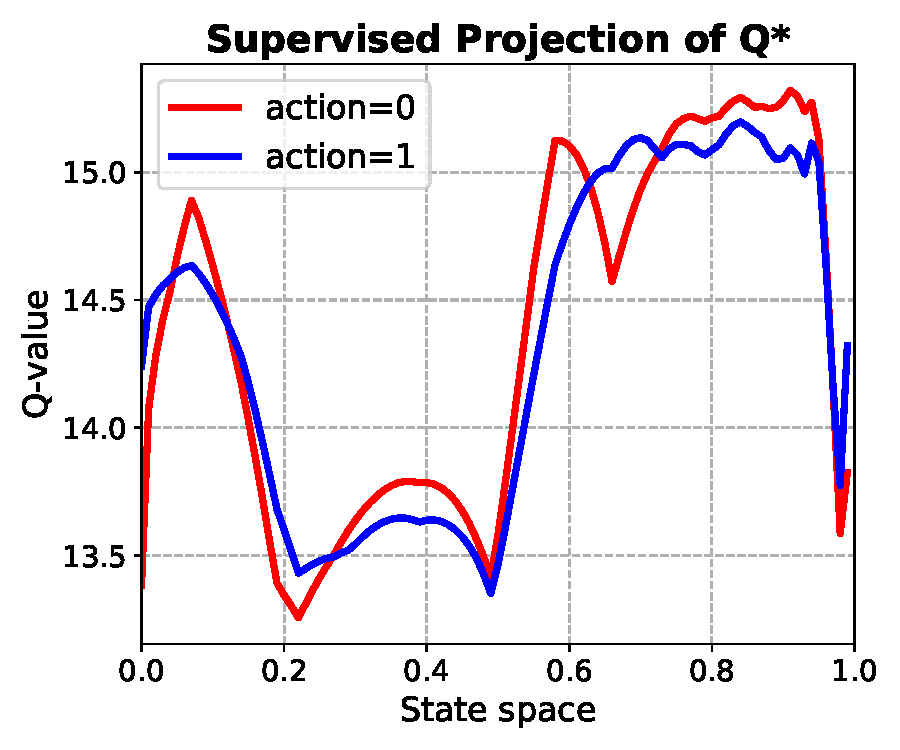
\includegraphics[width=0.48\linewidth]{section3_figs/supervised_q.pdf}
    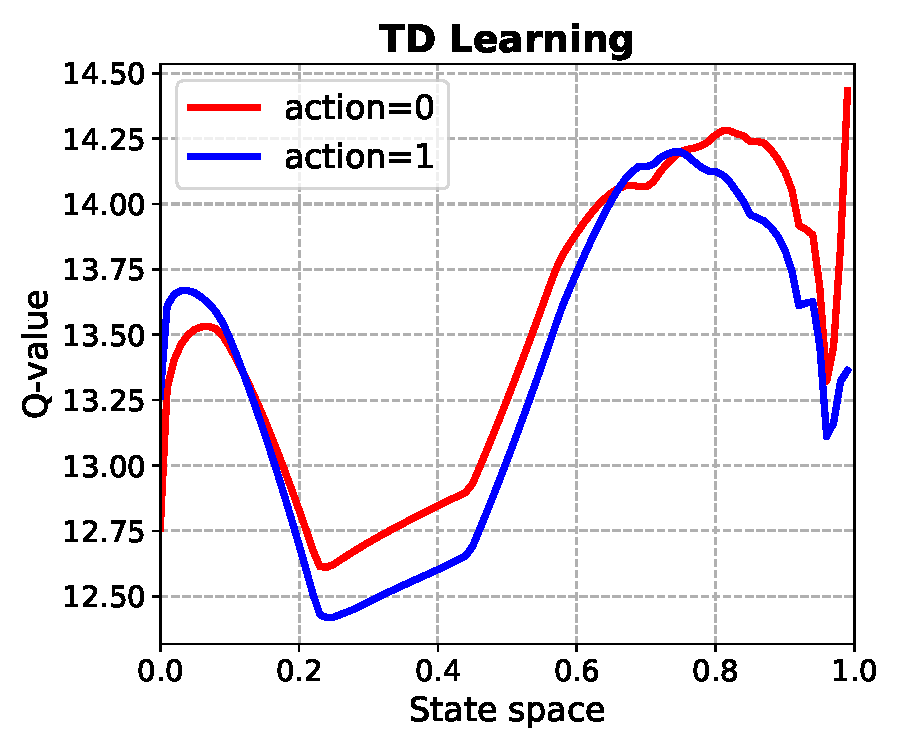
\includegraphics[width=0.48\linewidth]{section3_figs/td_learning.pdf}
    \vspace{-0.21cm}
    \caption{\small{\textbf{TD-learning fails to represent high frequency changes in Q-functions much more than supervised learning.} On the 1D MDP (dynamics, top-left), TD learning ignores the high-frequency components of the Q-function leading to worse action selection compared to supervised regression.}} 
    \label{fig:1d_mdp}
    \vspace{-0.6cm}
\end{wrapfigure}
%%AK: Tengyu had an interesting suggestion here: represent the action choices of each function via a shaded interval on the the number line, using blue for a_0 and red for a_1. The number of switches will determine the complexity of the Q-function, and this will show that TD has 4 switches, supervised has 8 and actual has 12 or 13 switches.
\textbf{Inability to model high-frequency components of Q-function.} Prior work has noted that Q-functions can be highly non-smooth even when reward functions and dynamics are relatively simple~\citep{dong2020expressivity}.
%%AK: does gamma models also note something related to complexity of Q vs reward via the discount profile stuff?
Would feature co-adaptation lead the Q-function to ignore certain high-frequency components in the objective?
As a didactic example of this phenomenon, we utilize a 2-action MDP with a 1-D state space $\mathcal{S} \in [0, 1]$ from~\citep{dong2020expressivity}. This MDP exhibits a piecewise linear dynamics (Fig.~\ref{fig:1d_mdp}, top-left) and an identity reward function $r(\bs, \ba) = \bs$ with two actions $\ba \in \{0, 1\}$. The optimal Q-function exhibits high-frequency changes (Fig.~\ref{fig:1d_mdp}, top-right). We find that running Q-learning (Fig.~\ref{fig:1d_mdp}, bottom-right)
attains Q-functions that completely ignore these high-frequency changes. This often makes the resulting policy choose the worse action of the two possible actions. On the contrary, a supervised projection (Fig.~\ref{fig:1d_mdp}, bottom-left) of the Q-function does capture many of these high frequency shifts in the Q-function. To formalize this didactic example, we prove the following result showing that high-frequency components of the Q-function are not modelled as a direct consequence of Theorem~\ref{thm:aliasing_exists}. The proof and a complete statement for Theorem~\ref{thm:num_pieces} can be found in Appendix ??.

%%AK: this will have some conditions on dynamics too, maybe we mention that as a detail in the appendix? But if it is unclear, maybe we should add it here, and explain it here...
\begin{theorem}[Informal]
Assume that the state-space $\mathcal{S}$ of the MDP is given by the 1-D number line, and that the groundtruth Q-function is (approximately) piecewise linear in the state $s$ with $N^*$ pieces. Denote the (approximate) number of linear pieces in a learned infinite-capacity ReLU Q-network via direct supervised regression as $N_{\mathrm{Sup}}$ and via TD-learning as $N_{\mathrm{TD}}$. Then: $N_{\mathrm{TD}} \leq N_{\mathrm{Sup}} \leq N^*$.     
\label{thm:num_pieces}
\end{theorem}
%%AK: In the proof of this theorem, we show this for approximate number of pieces, which is the integral of the second derivative of the function w.rt.t the input over the input space, but I think going into details would just hurt understanding here.

%%AK: I am a little unsure about the following part, in the sense if we should have it or not? This might seem obvious to some extent? 
% \textbf{Severe co-adaptation renders distributional shift corrections ineffective.} To test whether offline RL corrections alleviate feature co-adaptation, we performed a controlled experiment -- we constrained offline RL regularizers to only control the last linear layer of the Q-network, whereas bootstrapping was allowed to train the entire network. While we might expect that offline RL methods may still be effective by adapting the last weight layer to the features, contrary to this expectation, as shown in Figure ??, we find that all such variants (denoted as CQL($\phi$)) perform extremely poorly compared to the complete offline RL method. Further note the inability to minimize the regularizer corresponding to distributional shift and an increased dot-product similarity, $\Delta(\bs, \ba, \bs', \ba')$. This indicates that feature co-adaptation can lead to failure of offline RL methods. \textcolor{red}{add new figure for this}
%%AK: If we do keep this, maybe we should also add some line to justify why offline RL methods are still sensitive -- this is because they are not exactly doing SARSA?

\textbf{Lack of stability near ``good'' Q-function solutions.}
%%SL.5.22: instead of using a vague term like "good" with scare quotes, can we just say optimal? And what does "lack of stability" mean? Maybe just state it directly: Implicit regularization can prevent convergence, even when initializing at an optimal solution. [or something like that]
Finally, we study if co-adaptation of features cause the TD-learning process to diverge away, even when initialized favorably in the vicinity of a good Q-function (e.g., one obtained via supervised regression to MC returns or one obtained via online RL). Running Q-learning from such a favorable initialization eventually produces solutions that perform poorly as shown in Figure ?? below. Moreover, \textcolor{red}{say something about ranks here}. Indeed, in accordance with Theorem~\ref{thm:aliasing_exists}, the feature co-adaption phenomenon drives learning towards solutions with lower $\srank(\bM_{\mathrm{TD}}(\phi))$ values, giving rise to poor performance. \textcolor{red}{add figure, theorem}      
\fi

%%SL.5.17: what are Bellman constraints?
% are only enforced approximately (i.e., when the TD error
% %%SL.5.17: was the TD error ever defined?
% is not exactly 0), the implicit regularization towards minimum $||\bw||_2$ norm solutions will lead to the Q-function ignoring high-frequency components. That is, if the true Q-function changes dramatically from one state to the next, low TD-error solutions will fail to represent these changes.
%%SL.5.17: I don't see why the above theorem indicates that this is true
%%AK: add a worst-case theorem as discussed with George today?
%%SL.5.17: maybe we should put this didactic example into a separate \paragraph{} with more setup, instead of presenting this as a kind of footnote -- as-is, I think many people will not really understand it


%%AK: Check if we can take this paper's "peicewise linear theory" and convert it to a policy improvement bound differentiating between TD and supervised, as opposed to just fitting Q*-values?

% \subsection{Consequences of Overly Regularized Representations in TD Learning}
% Having seen aliasing of features on state-action tuples used for bootstrapping emerge as one pathological consequence of overly regularized representations in TD-learning compared to supervised learning, we next ask the following question we study the impact of over-regularization have on the performance of TD-learning. In particular, we ask: do TD-learning algorithms find generalizing and stable optima? To answer these questions, we consider a simple scenario where learning is initialized from a 


% \textbf{Abstract model.} Our abstract model captures feature learning as making a discrete selection among $K$ different feature vector candidates, $\{\Phi_1, \Phi_2, \cdots, \Phi_K\}$, $\Phi_i \in \mathbb{R}^{|\data|\times d}$,
%%SL.5.13: It would be way easier to understand if we could get continuous domains, and then just frame this as an optimization over \Phi (i.e., optimization over \Phi corresponds to selecting the best \Phi \in [some set]), that way we don't have to have this "discrete selection" business and could just say that it's part of the optimization process.
% and then training a linear layer $\bw \in \mathbb{R}^{d}$ to obtain the Q-function.
%%SL.5.13: One way you could phrase is this: Our abstract model of the learning process separates the neural network into two parts: a representation $\Phi$ and a weight vector $\bw \in ...$, such that the full model is given by $\Phi(..)^T \bw$ (i.e., $\bw$ corresponds to the last linear layer). The learning process is framed as a \emph{bilevel} optimization problem, where the weights $\bw$ are chosen subject to a constraint that the learning process chooses the optimal features $\Phi \in [set]$ for $\bw$ (or something like that)
% To mimic the overparameterized nature of neural networks, we assume that we operate in the overparameterized regime with $n < d$.
%%SL.5.13: This is kind of weird -- usually the last layer features are not that high dimensional, but the model parameters are. Are you sure we shouldn't look for some way to "NTK-ify" this? Perhaps a better way to frame this is that we are in the NTK regime where the choice of Phi corresponds to the choice of NTK (i.e., it's not fixed, as is more common in this analysis), while bw corresponds to the neural net parameters? That would justify the overparameterized regime and make this less weird.
% Assume that the initial value of the weight vector $\bw^{(0)} = 0$. We then write out the minimum-norm optimization problem shown below in Equation~\ref{eqn:min_norm} that attains the same solution as the optimal solution found by minimizing training TD error in this model, and characterize the properties of features $\Phi_K^*$ that are selected to obtain the minimum-norm solution. \textcolor{red}{more assumptions?}     
%%SL.5.13: It won't be clear to some people what min-norm has to do with neural net training, can you cite something to justify this?
% \begin{align}
%     \min_{\bw, \boldm_i \in \{0^d, 1^d \}}~~& ||\bw||_2^2 \nonumber\\
%     \text{s.t.}~~&~ \bar{\Phi}^\top \bar{\Phi} \bw = \bar{\Phi}^\top R + \gamma \bar{\Phi}^\top P^\pi \bar{\Phi} \bw, ~~ \bar{\Phi} = \left[\Phi_1, \cdots, \Phi_k\right] \otimes [\boldm_1, \cdots, \boldm_K]
% \label{eqn:min_norm}
% \end{align}
%%SL.5.13: ouch, this \bm_i is... difficult to parse
% Our first result characterizes the feature representation $\bar{\Phi}$ -- equal to one of $\Phi_i$ selected based on the learned masks $\bm_i$ -- that satisfies the Bellman consistency condition but also minimize the implicit regularizer, $||\bw||_2^2$,
% %%SL.5.13: where does this implicit regularizer come from?
% and use this to depict the existence of this phenomenon.


\iffalse

\section{Representation Regularization in Offline Q-Learning}
\label{sec:problem}
%%SL.5.13: See my comment on the title about "excessive" (maybe we call it Implicit Over-Regularization?). That said, this again sounds *extremely* similar to IUP, to the point where the section title alone could lead many readers to suspect this is just a direct copy of the IUP paper.
%%AK: yeah I agree. I am a little unsure what to call it, besides maybe admitting that this is similar IUP in high-level motivation but not low-level technical details. Do you think that's doable? My rationale was that right now readers might have the impression that we are trying to do something like IUP but also trying to distinguish it from IUP, without making clear what our contribution is and what's already there. Perhaps just saying something like "Fine-grained analysis" or something that explicitly quantifies the extent of this contribution is different? Avoiding that might just create questions. What do you think?
%%AK: the title sounds lika having a good connotation, is there a bad word for "regularization" that is not just "over-regularization" or "aliasing"?

% In this section, we study the mechanism by which implicit regularization effects are induced in offline Q-learning, and discuss how these effects can lead to pathological issues such as overly aliased representations and convergence to poor solutions. These aliasing properties exist even when learning is initialized from good solutions that do not exhibit this aliasing, and can make the learning eventually diverge. We first provide an empirical analysis of this phenomenon and then theoretically formalize these observations in a simple abstract model of learning dynamics of Q-learning.
Offline RL algorithms discussed previously are unstable and suffer from hyperparameter tuning challenges. A simple choice such as the number of training steps can be game-changing -- too few gradient steps will of course give rise to underfitted Q-functions, but perhaps surprisingly, too many gradient steps also lead to poor performance (Figure~\ref{fig:atari_5_percent}, Figure 2 in \citep{kumar2021implicit}). This phenomenon resembles statistical overfitting at first, however, it is actually underfitting caused due to excessive representational regularization of training deep networks with TD error that manifests as aliased features. While this issue has been broadly noted in previous work~\citep{kumar2021implicit}, in this section we will provide a fine-grained analysis of this phenomenon first empirically and then theoretically. In Section~\ref{sec:method}, we will then discuss a simple regularization scheme that can mitigate this issue. \textcolor{red}{TODO}  
%%SL.5.13: Maybe a somewhat more forceful lead-in could look like this:
% While the offline RL algorithms discussed in the previous section mitigate the worst challenges of offline RL~\citep{bear}, effectively using such methods in practice still requires extensive hyperparameter tuning. A particularly delicate choice is the number of gradient steps to take on the offline dataset -- too few gradient steps obviously produce underfitted, suboptimal value functions. But surprisingly, too many gradient steps also often result in poor performance, as illustrated in Figure ??. What is the reason for this performance collapse? While this phenomenon initially resembles overfitting, it is in fact an instance of \emph{underfitting}: although deep networks trained with SGD should provide a very good fit in standard supervised settings, we will argue that training with TD backups introduces a pathological over-regularization effect, induces excessive aliasing, and greatly constrains the expressive power of the resulting features. We first analyze this empirically, and then present a theoretical analysis. In Section ??, we will discuss how a simple regularization scheme can mitigate this issue.
%%AK: I havent added this fully, and instead cited IUP for the basic "noting" of this phenomenon and then said that we provide finegrained analysis of it. But I can change it. 

\iffalse
\subsection{Empirical Analysis}
\label{sec:empirical_analysis}
\begin{wrapfigure}{r}{0.49\textwidth}
    \vspace{-47pt}
    \centering
    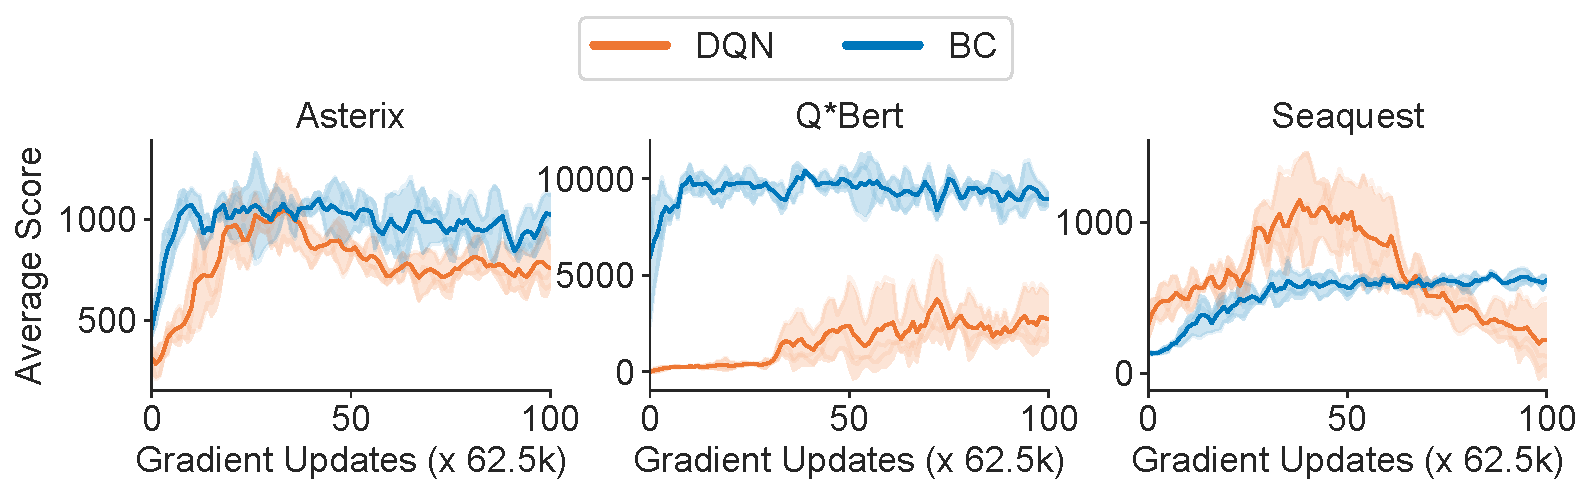
\includegraphics[width=\linewidth]{atari/perf_3_games.pdf}
    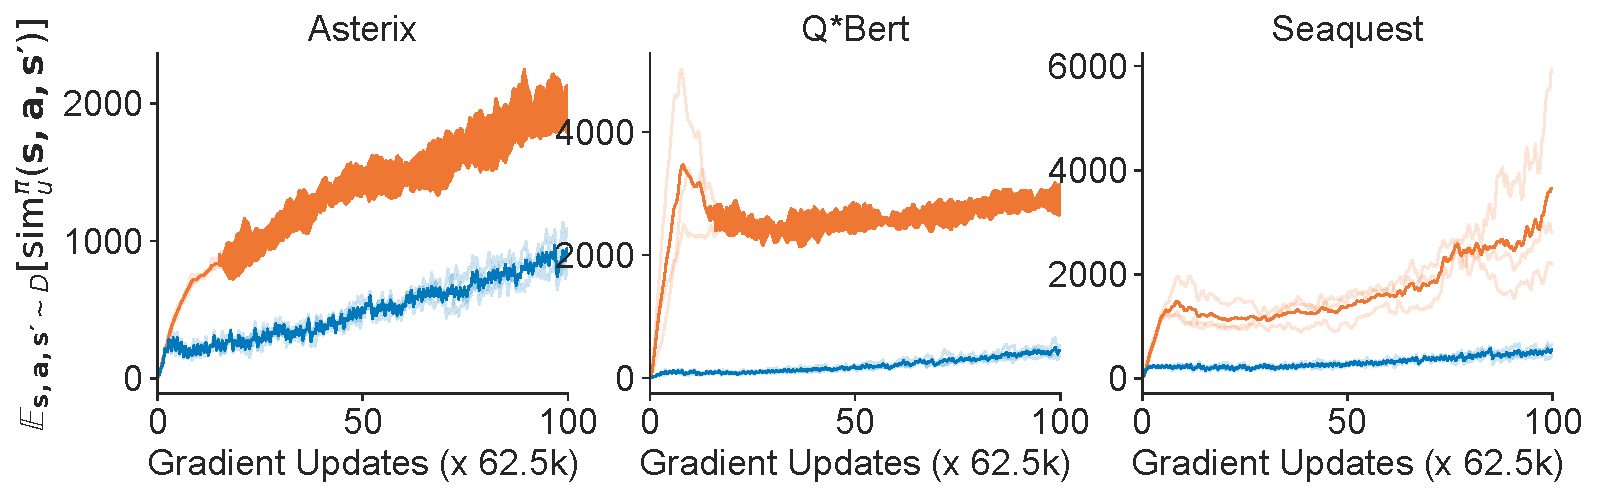
\includegraphics[width=\linewidth]{atari/unnorm_3_games.pdf}
    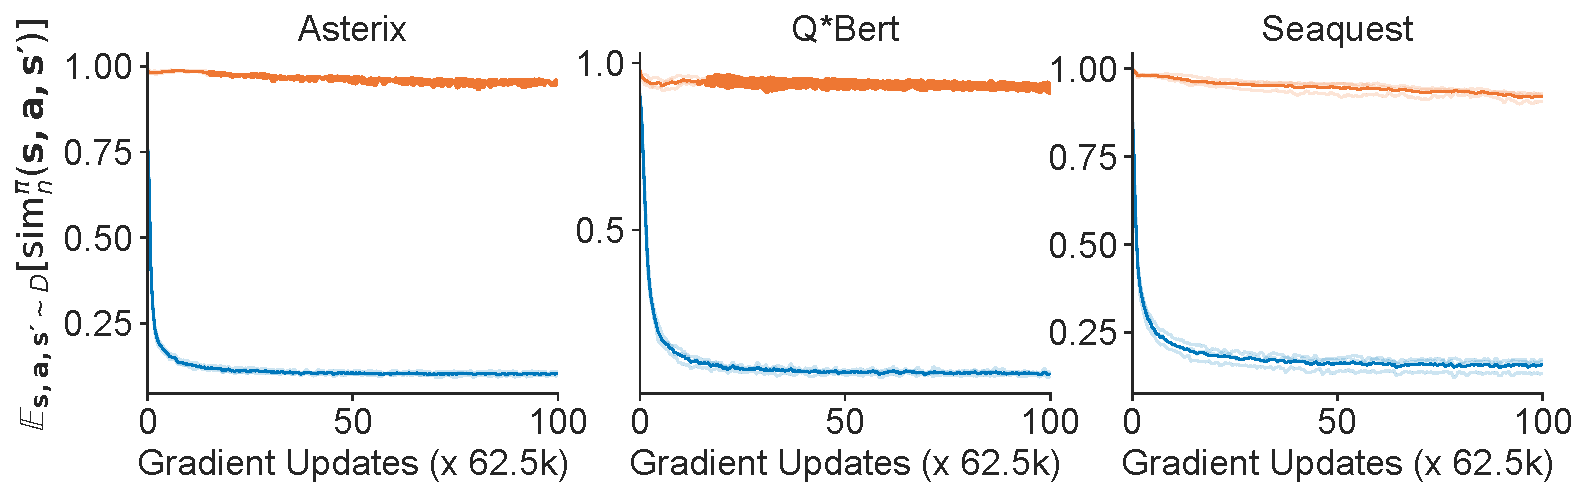
\includegraphics[width=\linewidth]{atari/norm_3_games.pdf}
    \vspace{-0.65cm}
    \caption{\small{Performance of offline DQN and BC on 5\% DQN replay dataset~\citep{agarwal2019optimistic} (top), normalized similarity scores for DQN and BC (bottom). As compared to DQN, $\simnorm$ (cosine similarity) decays significantly faster for BC. 
    \textcolor{red}{Remove the middle row that's not useful. Reduce to 2 games. Also add SARSA}}
    } 
    \label{fig:atari_3_games}
    \vspace{-0.4cm}
\end{wrapfigure}
%% The first para is saying aliasing exists in very simple language
%%SL.5.13: I think before we dive into why it happens, can we just show what the problem is? E.g., show some learning curves where performance peaks and drops, and explain what's going on. Only then talk about *why* it happens
%%AK: sorry for bringing this up again. But I feel like that would make it like iUP basically. I have cited this issue of what happens using a figure later in the paper in the para above as well as citing figure from IUP. We can put a wrapfig in the accompanying text above, but it feels a little copied if we spend the technical section on this. Maybe this is not a good choice. What do you think? 
As noted in~\citep{kumar2021implicit}, one of the most notably visible impacts of representation regularization is the pathological feature aliasing phenomenon that arises with more training. While this aliasing issue has been previously quantified via a collapse in the rank of the feature matrix $\Phi$, this evidence does not shed light on the exact mechanism by which aliasing happens -- even standard supervised learning would exhibit a drop in rank($\Phi$); though not in enormous amounts. % one closing line on how as a result it is less clear how to measure aliasing and connection to bootstrapping empirically.   
%%AK: tried to add a comparison against 

\textcolor{red}{This first part of Section 3.1 will likely be removed in favor of a didactic example} \textit{How can we connect the degree of aliasing to bootstrapping?} Since the difference between bootstrapping and standard supervised learning is primarily that the Q-function at $(\bs, \ba) \in \mathcal{D}$ is trained  with targets generated using Q-values at $(\bs', \ba')$ instead of fixed targets, excessive similarity between $\phi(\bs, \ba)$ and $\phi(\bs', \ba')$ leads to highly coupled Q-values on the two sides of the Bellman update, which can lead to issues such as overestimation and divergence~\citep{durugkar2018td}. Hence, it is informative to measure the similarities in representations $\phi(\bs, \ba)$ and $\phi(\bs', \ba')$. We measure two notions of similarity: \textbf{(1)} we measure the cosine similarity between $\phi(\bs, \ba)$ and $\phi(\bs', \ba')$, and \textbf{(2)} we measure an aggregate    

Observe in  Figure~\ref{fig:atari_3_games} that perhaps surprisingly the similarity between $\phi(\bs, \ba)$ and $\phi(\bs', \ba')$ decreases and saturates at low values with behavior cloning (BC),
%%SL.5.13: This feels like a non-sequitur -- you're comparing representations at two different states, why does it matter that BC is trying to match the behavior policy?
On the other hand, DQN, which is trying to actually improve upon the behavior policy, essentially aliases
%%SL.5.13: There is no evidence of aliasing, just of high dot product (which is not the same)
feature representations at $(\bs, \ba)$ and $(\bs, \ba')$, giving rise to very high similarity values.
%%SL.5.13: Without more context about what's going on, I would say at this point that this is probably due to the OOD actions problem you mentioned before, which DQN does nothing to fix. Additionally, I think it's very likely that many reviewers at this point woudl complain that it's non-sensical to compare BC (which learns policies) with DQN (which learns Q-functions).
This indicates that, compared to supervised learning (e.g., BC), implicit regularization effects in deep Q-learning have a tendency to alias predictions at states and corresponding next states. \textcolor{red}{Would be good to show this with SARSA vs MC: that way we can make a stronger statement like: Note that while both SARSA and MC returns are essentially computing the same quantity and differ only in the nature of implicit regularization induced. This difference makes a huge difference -- in one case, representations at consecutive states are essentially completely aliased, while supervised learning is able to disentangle representations.}
%%SL.5.13: Overall, I think this paragraph is rather problematic. If you want to explain this part, it would be good to really slow it way down and walk the reader through it much more slowly, otherwise so many of the choices in the above paragraph come across as ad hoc, making the conclusions unconvincing.

\fi

\subsection{A Didactic Example}
\label{sec:empirical_analysis}

As noted in~\citep{kumar2021implicit}, one of the most notably visible impacts of representation regularization is the pathological feature aliasing phenomenon that arises with more training. While this aliasing issue has been previously quantified via a collapse in the rank of the feature matrix $\Phi$, this evidence does not shed light on the exact mechanism by which aliasing happens -- even standard supervised learning would exhibit a drop in rank($\Phi$) with more training, and while prior work shows that bootstrapping exacerbates it empirically, it is unclear how exactly this amplification happens. In this section, we describe the intuition behind this mechanism with a didactic example of a 2-action, 1D line MDP~\citep{dong2020expressivity} with a piece-wise linear deterministic dynamics function, $P(\bs'|\bs, \ba) = \mathbb{I}(\bs' = f(\bs, \ba))$ shown in Figure ??. The reward $r(\bs, \ba)$ at any state is the value of the state itself, i.e., $r(\bs, \ba) = \bs$.

The optimal Q-function for this MDP is shown in Figure ??, and 3-layer deep ReLU network Q-functions estimators learned via supervised regression and TD-learning on the identical finite dataset are shown respectively in Figures ?? and ??. While neither supervised regression nor TD learning can learn the complete structure of the optimal Q-function, TD learning fails to represent important high-frequency components of the Q-function (marked in yellow), leaning a ``simple'', smooth Q-function. Since it fails to model the changes in the Q-function well, the resulting policy often chooses the worse action. Quantitatively, the policy extracted from such a TD Q-function is worse than that extracted from the supervised Q-function at more than half the states.  
%%AK: todo: mark in yellow via keynote

%% The next para is saying aliasing is undesirable
\textbf{Why do we observe overly smooth Q-functions in the didactic example when trained with TD learning?}  While excessive aliasing of internal representations in the neural network is expected to generally lead to poor performance, aliasing between $\phi(\bs, \ba)$ and $\phi(\bs', \ba')$ is especially detrimental when learning with Bellman backups. Intuitively, since Bellman backups train features such that the difference of Q-values, $Q(\bs, \ba) - \gamma Q(\bs', \ba')$ matches the reward function, $r(\bs, \ba)$, only on a finite number of state-action tuples seen in the dataset, the features $\phi(\bs, \ba)$ and $\phi(\bs', \ba')$ can learn to only be sufficiently different to predict the reward, thereby achieving low TD error and may be excessively regularized otherwise, thus not capturing long-term structure in the Q-function. Put in other words, there are many possible assignments of weights to a function approximator that could give rise to equally low TD error at the cost of varying degrees of aliasing or regularization.

%%SL.5.13: This feels really hand-wavy. I'm also not sure I agree with this argument -- after all, how would it be any different if there *wasn't* aliasing? Wouldn't you still get a good fit between the difference and reward? This kind of a makes a non-falsifiable statement.
%%AK: this figure is like the example in the MB vs MF paper, but with Bellman backups run on it.

\begin{wrapfigure}{r}{0.5\textwidth}
    \centering
    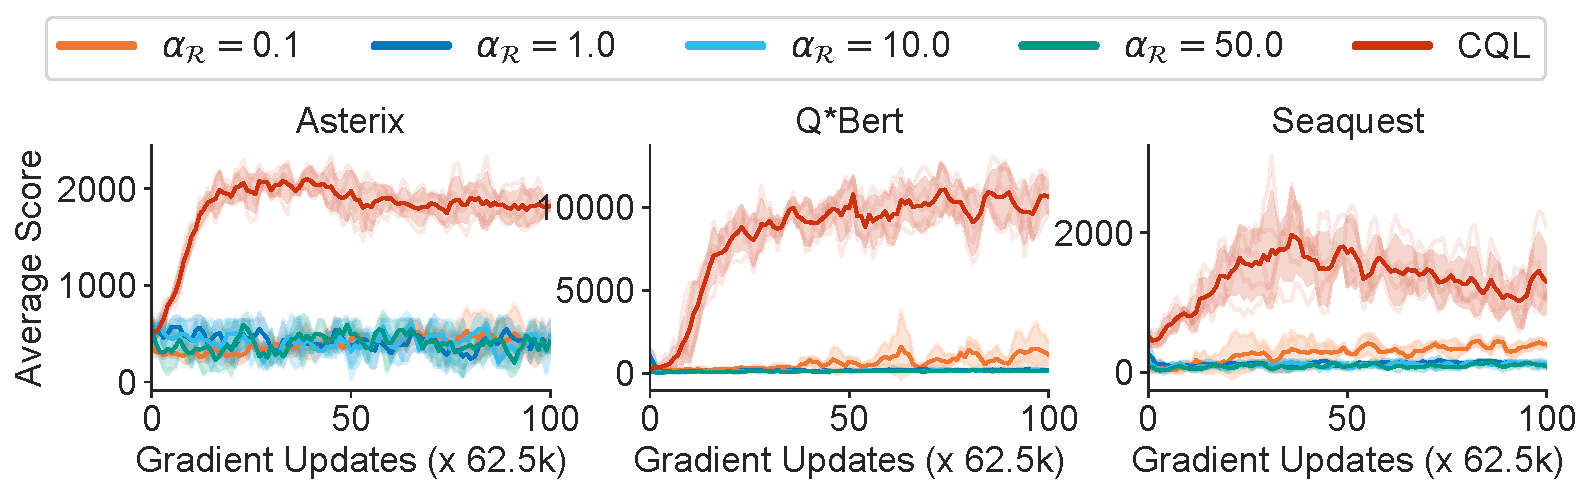
\includegraphics[width=\linewidth]{atari/cql_on_bootstrapping_feat.pdf}
    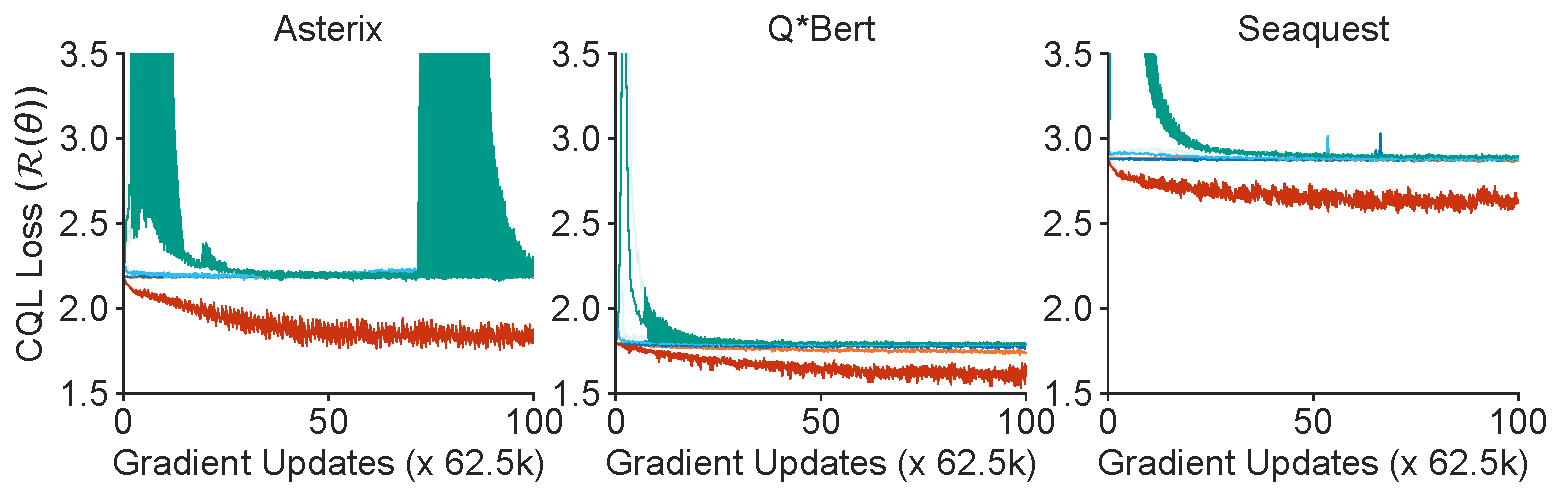
\includegraphics[width=\linewidth]{atari/cql_losses_bootstrapped_feat.pdf}
    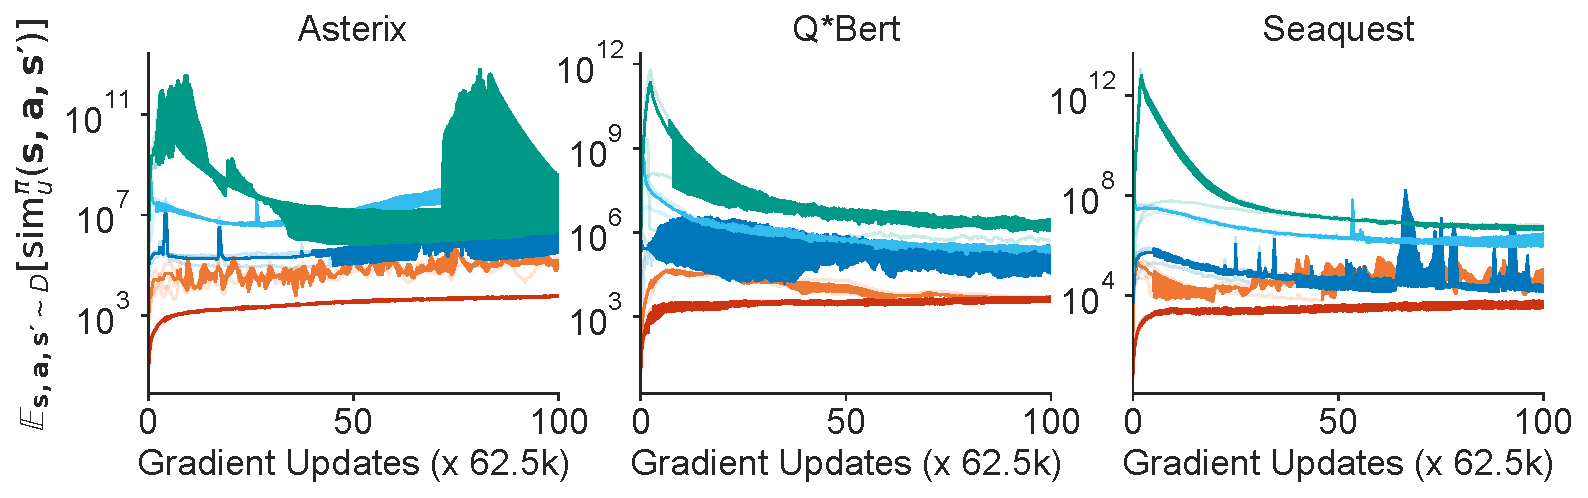
\includegraphics[width=\linewidth]{atari/sim_s_ns_cql_on_bootstrapping_feat.pdf}
    \vspace{-0.65cm}
    \caption{\small{CQL($\phi$), trained using 5\% DQN replay dataset, that learns on features trained solely via bootstrapping where the CQL regularizer $\mathcal{R}(\theta)$ only updates the linear weights of the Q-network. Different values of $\alpha_R$ correspond to different strengths of conservative regularization. We also show standard CQL~(red) for comparison.}} 
    \label{fig:atari_3_games_cql_bootstrap}
    \vspace{-0.6cm}
\end{wrapfigure}
When excessive aliasing is induced by such a mechanism, even modern offline RL methods that are meant to prevent against distributional shift
%%SL.5.13: It's unclear what preventing distributional shift has to do with this
are rendered ineffective. To demonstrate this empirically, we trained a modified version of CQL~\citep{kumar2020conservative}, CQL$(\phi)$, that learns on features $\phi(\bs, \ba)$ solely trained via bootstrapping, and the CQL regularizer is allowed to only update the last linear layer weights. As shown in Figure~\ref{fig:atari_3_games_cql_bootstrap}, no strength of conservative regularization is able to minimize out-of-distribution Q-values resulting in higher values of CQL loss and significantly worse performance as compared to CQL. This indicates that, no matter what, aliased representations can significantly hamper the efficacy of offline RL methods.
%%SL.5.13: This experiment seems weird. You said (and showed before) that features learned with bootstrapping are bad, and it seems like now you are saying if you take those features and retrain, it's still bad, but that's not surprising. I think the subtlety here is that you are also showing that the CQL regularizer is ineffective, but that seems obvious? And it also requires a degree of familiarity with CQL to understand, that the reader might not have. Maybe we can do away with this paragraph?

%%AK: this is the experiment where we initialize the Q-function from a good checkpoint and show it still performs poorly so it is reasoning about the stability aspect.
Finally, to demonstrate the detrimental extent of this implicit regularization on stability of the offline RL algorithm, we perform a controlled experiment where Q-learning is initialized from a ``good'' Q-function that doesn't exhibit aliasing.
%%SL.5.13: where does this come from?
As shown in Figure ??,
%%AK: TODO(AK): add figure!
more learning iterations with modern offline RL algorithms can still drive the algorithm away from this good solution towards more aliased and poor performing solutions. This shows that aliasing caused due to the implicit regularization of training does not just affect the peak performance of an algorithm, but also plays a significant role in destabilizing algorithms when they reach their peak performance.  

\subsection{Theoretical Analysis of Implicit Regularization in Offline Deep Q-Learning}
\label{sec:theory_evidence}
%%SL.5.13: Calling this "implicit regularization" seems premature -- all we showed is that features get larger dot products, which doesn't mean there is some sort of "implicit regularization" going on
In this section, we formalize our empirical observations from Section~\ref{sec:empirical_analysis} and provide a theoretical analysis of the implicit regularization issue. We aim to answer two questions: \textbf{(1)} How do implicit regularization effects in TD learning affect the the aliasing of representations at consecutive states used in the Bellman update? and, \textbf{(2)} How does excessive aliasing affect performance of the algorithm? To answer these questions, we first introduce a simple abstract model of neural network behavior
%%SL.5.13: Rephrase as something like: we first introduce a simple abstract model of neural network training dynamics in value-based RL, and then use this model to analyze the effect of repeated SGD updates on the TD objective. [or something like that]
that allows us to answer these questions.

% abstract model
%% AK: TODO (AK): Also check if we can generalize this to arbitrary continous domains
%%SL.5.13: In its current form, I'm a bit nervous about this version of the theory. I think the SGD implicit regularization version is more convincing and makes fewer arbitrary choices. I do think this version could be made better if we can get rid of the discrete set though. Would be good to get Tengyu's take on it too...
\textbf{Abstract model.} Our abstract model captures feature learning as making a discrete selection among $K$ different feature vector candidates, $\{\Phi_1, \Phi_2, \cdots, \Phi_K\}$, $\Phi_i \in \mathbb{R}^{|\data|\times d}$,
%%SL.5.13: It would be way easier to understand if we could get continuous domains, and then just frame this as an optimization over \Phi (i.e., optimization over \Phi corresponds to selecting the best \Phi \in [some set]), that way we don't have to have this "discrete selection" business and could just say that it's part of the optimization process.
and then training a linear layer $\bw \in \mathbb{R}^{d}$ to obtain the Q-function.
%%SL.5.13: One way you could phrase is this: Our abstract model of the learning process separates the neural network into two parts: a representation $\Phi$ and a weight vector $\bw \in ...$, such that the full model is given by $\Phi(..)^T \bw$ (i.e., $\bw$ corresponds to the last linear layer). The learning process is framed as a \emph{bilevel} optimization problem, where the weights $\bw$ are chosen subject to a constraint that the learning process chooses the optimal features $\Phi \in [set]$ for $\bw$ (or something like that)
To mimic the overparameterized nature of neural networks, we assume that we operate in the overparameterized regime with $n < d$.
%%SL.5.13: This is kind of weird -- usually the last layer features are not that high dimensional, but the model parameters are. Are you sure we shouldn't look for some way to "NTK-ify" this? Perhaps a better way to frame this is that we are in the NTK regime where the choice of Phi corresponds to the choice of NTK (i.e., it's not fixed, as is more common in this analysis), while bw corresponds to the neural net parameters? That would justify the overparameterized regime and make this less weird.
Assume that the initial value of the weight vector $\bw^{(0)} = 0$. We then write out the minimum-norm optimization problem shown below in Equation~\ref{eqn:min_norm} that attains the same solution as the optimal solution found by minimizing training TD error in this model, and characterize the properties of features $\Phi_K^*$ that are selected to obtain the minimum-norm solution. \textcolor{red}{more assumptions?}     
%%SL.5.13: It won't be clear to some people what min-norm has to do with neural net training, can you cite something to justify this?
\begin{align}
    \min_{\bw, \boldm_i \in \{0^d, 1^d \}}~~& ||\bw||_2^2 \nonumber\\
    \text{s.t.}~~&~ \bar{\Phi}^\top \bar{\Phi} \bw = \bar{\Phi}^\top R + \gamma \bar{\Phi}^\top P^\pi \bar{\Phi} \bw, ~~ \bar{\Phi} = \left[\Phi_1, \cdots, \Phi_k\right] \otimes [\boldm_1, \cdots, \boldm_K]
\label{eqn:min_norm}
\end{align}
%%SL.5.13: ouch, this \bm_i is... difficult to parse
Our first result characterizes the feature representation $\bar{\Phi}$ -- equal to one of $\Phi_i$ selected based on the learned masks $\bm_i$ -- that satisfies the Bellman consistency condition but also minimize the implicit regularizer, $||\bw||_2^2$,
%%SL.5.13: where does this implicit regularizer come from?
and use this to depict the existence of this phenomenon.

\begin{theorem}
\label{thm:aliasing_exists}
Let the singular value decomposition of $\Phi_i$ be given as $\Phi_i = \bU_i \Sigma_i \bV_i^\top$ and $\bw^{(*)}, \boldm^{(*)}$ minimize the objective in Equation~\ref{eqn:min_norm}. Assume that the reward vector lies in the column space of $\Phi_i$, $\forall i \in [K]$, i.e., $\exists~ y_i, R = \Phi_i y_i $.  Then, $\bar{\Phi}$ is such that:
\begin{equation*}
    \bar{\Phi} := \arg \min_{i}~ \big|\big| \Sigma_i^{-1} \left( \bU_i^T (I - \gamma P^\pi) \bU_i \right)^{-1} \Sigma_i y_i\big|\big|_2^2.
\end{equation*}
Thus, the resulting $\bar{\Phi}$ satisfies: $\mathrm{srank}\left(\bar{\Phi}^\top (\bar{\Phi} - \gamma P^\pi \bar{\Phi}) \right) \leq \mathrm{srank}\left(\Phi_i^\top (\Phi_i - \gamma P^\pi \Phi_i) \right)~ \forall i$, which quantifies the existence of aliasing between representations at consecutive states in TD-learning.
\end{theorem}
%%SL.5.13: It's not clear what this last sentence means ("which quantifies the existence of aliasing between representations at consecutive states in TD-learning") -- can we state the implication of this theorem more precisely. As written, it's also not clear what this theorem has to do with SGD (I guess it's the min-norm part?).

%%SL.5.13: It might also help with clarity to explain why this problem *doesn't* happen in the supervised learning case

A proof of Theorem~\ref{thm:aliasing_exists} can be found in the Appendix ??. The main consequence of this result is a characterization of the learned features at optimal TD solutions in our abstract model in terms of the effective rank~\citep{kumar2021implicit} of the matrix $\bM(\Phi) := \Phi^\top (\Phi - \gamma P^\pi \Phi)$. A low rank of $\bM(\Phi)$ for a given rank of $\Phi$ intuitively indicates that the basis of the difference in features at consecutive states, $\Phi - \gamma P^\pi \Phi$, heavily lies
%%SL.5.13: try to avoid hand-wavy language ("heavily lies") and state what you mean more precisely
in the null space of the feature matrix $\Phi$, as a result of which the weight vector $\bw$ will be updated only in a few directions allowed by both $\Phi$ and $\Phi-\gamma P^\pi \Phi$.indicating that only a partial set of features will actually be used for learning.
%%SL.5.13: something is malformed above ("indicating that")
To empirically verify the existence of such an aliasing phenomenon, following the procedure outlined in \citep{kumar2021implicit}, we measure the effective rank of $\bM(\Phi)$ and observe in Figure ?? that this matrix indeed has extremely low rank when training with TD backups, as compared to supervised regression.
%% AK: this supervised regression is BC. Should we also do this for something else?

%%AK: maybe write the stuff below as a theorem?
Another interesting consequence of Theorem~\ref{thm:aliasing_exists} is the effect of the ``simplicity'' of the reward function on feature aliasing. We define simplicity by the number of non-zero components in the vector $y_i$.
%%SL.5.13: maybe we should avoid ad hoc definitions like this, and try to just state this more plainly and directly?
As an extreme case, note that if the vector $y_i$ has all zeros, except a single 1 entry, the optimal $\bar{\Phi}$ is expected to induce $\bM(\Phi)$ with a much lower rank compared to when a significantly more number of values of $y_i$ are non-zero (as shown in Appendix ??).
%%SL.5.13: this seems imprecise ("much lower")
This means that when the reward function $R$ actually non-trivially combines the singular vectors of $\Phi$ -- which we refer to as a ``complex'' reward function -- the effective aliasing
%%SL.5.13: I think if you're going to use the term "aliasing" like this, it needs to be formally defined. Aliasing means that two things are indistinguishable (not similar, but indistinguishable). The word is being used in a different way here.
is little less than when it does not. We indeed observe this behavior in practice, as shown in Figure ?? in Section~\ref{sec:empirical_analysis}, and our abstract model sheds light on how this implicit regularization effect in TD-learning is exacerbated in scenarios where reward functions can be expressed using very few components of the feature matrix $\Phi$.
%%SL.5.13: how do you know if it can be expressed using very few components?
%%SL.5.13: I think I understand what you are trying to say in the above paragraph, but we need to find a cleaner and more concise way of saying it. Maybe what we can say is something like -- consider the projection of the reward function onto the column-space [?] of Phi, with coefficients ??. If these coefficients are sparse, we would expect [??] (try to be precise!)...

To conclude our analysis for question \textbf{(1)}, we finally note that an analogous result in supervised learning would indicate no existence of any implicit bias that preferentially aliases feature representations at consecutive states. While prior work \citep{kumar2021implicit} has also generally shown the compounding effect of implicit regularization towards low-rank $\Phi$ in TD-learning, our analysis explicitly identifies the structure of aliasing induced by this implicit regularization: the rank of the matrix $\bM(\phi)$ drops, leading to aliasing at consecutive states.
%%SL.5.13: It's good to have a paragraph like the one above, but it addresses two things simultaneously, and doesn't do either very well: the supervised learning bit seems to have no punchline (so... is this a contradiction? if not, why not?); the bit about IUP doesn't clearly state how what you are showing is different from IUP.

%%SL.5.13: Given how long-winded the above is, maybe consider a subsection heading for (2) or something (or at least paragraph heading)
Next, we answer question \textbf{(2)} regarding the detrimental impacts of aliasing. 
\textcolor{red}{Need to finish this bit -- there are some options we can go: (1) We can show that there exist MDPs with simple reward functions and complex Q-functions, where such an implicit regularizer will cause the MDP to learn overly smooth Q-functions. (2) We can show that even when initialized close to a good solution, this implicit regularizer will drive the model towards picking features that are the most aliased, in which case we do not even stabilize near a good solution even if we reach it. (3) We could show that distributional shift correction on top of aliased features will not work, similar to what we had before the ICML deadline. Which of these option(s) should we prefer?}

\fi






















%%%%%%%%%%%%%%%%%%%%%%%%%%%%%%%%%%%%%%%%%%%%%%%%%%%%%%%%%%%%%%%%%%%%%%%%%%%%%%%%
%%%%%%%%%%%%%%%% old stuff below %%%%%%%%%%%%%%%%%%

\iffalse
\section{\AliasingProblemName\ in Offline RL}
\label{sec:problem}
%%SL.2.3: Kind of a nitpick, but "Bootstrapping Aliasing" kind of makes it sound like we are bootstrapping the aliasing (rather than that we have aliasing that stems from bootstrapping). But why do you want "bootstrapping" in the name? It doesn't really have anything to do with bootstrapping, at least not moreso than anything else that relates to RL. It's kind of more like Policy Aliasing (or something like that...)

Empirically, we find that the combination of neural network function approximators, bootstrapping, and minimizing TD error 
% with gradient descent 
leads to aliasing
%%SL.2.3: Aliasing between what and what?
of the state-action pairs appearing in a Bellman update. Minimizing TD error against bootstrapped targets uses a tuple $(\bs, \ba, \bs')$ from the dataset, draws an additional action sample from $\pi(\cdot | \bs')$, which may not be observed in the dataset, and evaluates $Q_\theta(\bs, \ba)$ and $Q_\theta(\bs', \ba')$. We find that the features $\phi(\bs, \ba)$ and features $\phi(\bs', \ba')$ become aliased over the course of learning,
%In this section, we will see how offline training of Q-functions by minimizing TD error against a bootstrapped target value estimate \emph{aliases} feature representations on actions drawn from the dataset $\phi(\bs, \ba)$ and the feature representations on actions from the learned policy that will be used for bootstrapping, but are not observed in the dataset, which we denote as $\phi(\bs', \ba')$. Since features $\phi(\bs', \ba')$ directly influence the features at dataset state-action tuples $\phi(\bs, \ba)$ via the bootstrapping update, a similarity between features at these specific state-action tuples is likely to affect optimization dynamics of the algorithm as we will more formally discuss in Proposition~\ref{thm:separability}.  
%%AK.2.3: I don't know how to motivate this, I wrote something up but this isnt convincing 
%%SL.2.1: which we denote as
and we refer to this phenomenon as \emph{\aliasingproblemname}.
%%SL.2.3: As stated, this sounds a little bit silly, because \bs and \bs' are very similar, so of course they are likely to be aliased! I think it would help to explain the *policy* aliasing part first, and then explain that a particularly prominent instance of this has to do with \ba and \ba' (but FWIW, I still think we are making too big of a deal out of the fact that these are sequential actions, and things would be much clearer and less likely to be misunderstood if we did not do this, and instead focused on policy aliasing and brought in the s/a/s'/a' stuff as late as possible)
To measure this aliasing, we use the normalized and unnormalized dot product similarities %To begin, we formally define two metrics to quantify \aliasingproblemname, and then demonstrate the existence of this issue in offline Q-learning methods.
\begin{align*}
    \simnorm(\bs, \ba, \bs'; \phi) &:= \frac{|\phi(\bs, \ba)^T \E_{\pi(\ba'|\bs')}[\phi(\bs', \ba')]|}{||\phi(\bs, \ba)||_2 ||\E_{\pi(\ba'|\bs')}[\phi(\bs', \ba')]||_2},\\
    \simunnorm(\bs, \ba, \bs'; \phi) &:= |\phi(\bs, \ba)^T \E_{\pi(\ba'|\bs')}[\phi(\bs', \ba')]|.
\end{align*}
%\begin{definition}
%\emph{\Aliasingproblemname} is said to happen when features $\phi(\bs, \ba)$ on $(\bs, \ba, \bs') \in \data$ and the expected feature vector on actions drawn from the learned policy $\pi(\cdot |\bs')$ at the next state $\bs'$, $\E_{\ba' \sim \pi(\cdot|s')}[\phi(\bs', \ba')]$, exhibit a high normalized or unnormalized dot product similarity on an average over the dataset $\mathcal{D}$. The normalized ($\simnorm$) and unnormalized ($\simunnorm$) similarities are given by:
%%%SL.2.1: It's unclear why you are using a/a' on successive timesteps. Since this is a definition, it might come across as weirdly arbitrary. Beyond this, there is the question of whether this is referring to this quantity in expectation over s, on average, etc.
%%%AK.2.3: I don't know how best to do that. I want to write this section as policy indistinguishability, where we measure (s, a), (s, a') similarity, but that doesn't seem to be the case we can make in time
%\begin{align*}
%    \simnorm(\bs, \ba, \bs'; \phi) &:= \frac{|\phi(\bs, \ba)^T \E_{\pi}[\phi(\bs', \cdot)]|}{||\phi(\bs, \ba)||_2 ||\E_{\pi}[\phi(\bs', \cdot)]||_2},\\
%    \simunnorm(\bs, \ba, \bs'; \phi) &:= |\phi(\bs, \ba)^T \E_{\pi}[\phi(\bs', \cdot)]|.
%\end{align*}
%\end{definition}
We omit $\phi$ when it is clear from context. %A high $\simnorm$ indicates state-action tuples $(\bs, \ba) \sim \mathcal{D}$ and the next state-action tuple, $(\bs', \ba')$ where $\ba' \sim \pi(\cdot|\bs')$ are directionally aligned,
%%SL.2.1: Above sentence appears to (intentionally?) omit saying what the state is, just saying the action. Especially combined with the s/s'/a/s' confusion in the previous definition, this might be not so great
%%AK.2.3: added this 
%whereas the feature magnitude captured in $\simunnorm$ indicates the extent to which directional similarity affects optimization~(Section~\ref{sec:analysis}). As a result, by tracking average similarities over the dataset, $\E_{\bs,\ba, \bs' \sim \data}[\simnorm(\bs, \ba, \bs')]$ and $\E_{\bs, \ba, \bs' \sim \data}[\simunnorm(\bs, \ba, \bs')]$,
%%SL.2.1: This average thing seems a bit hacky.
%%AK.2.3: introduced the average bit in the definition above
%we can verify the existence of \aliasingproblemname.
Intuitively, this could be problematic in the offline RL setting where carefully controlling generalization is critical to performance~\citep{levine2020offline}
%%SL.2.3: I don't really understand what claim this reference is supposed to be supporting
because it couples the $Q$ values of $(\bs, \ba)$ and a potentially out-of-distribution tuple $(\bs', \ba')$.
%%SL.2.3: should clarify that it's the action that's OOD, not the state (lest someone misunderstand)
% For example, assume that the features $\phi(\bs, \ba) \in \mathbb{R}^d$ are positive (as is the case with ReLU activations) and unit norm, then $\simnorm(\bs, \ba, \bs') \geq 1 - \varepsilon$ immediately implies that $(Q_\bw(\bs, \ba) - \E_{\pi(\ba'|\bs')}\left[Q_\bw(\bs', \ba')\right])^2 \leq 2\varepsilon||\bw||_2^2$.
%%SL.2.3: This early in the paper, the significance of this inequality is not clear (indeed, it's not clear to me even, and I've read the whole paper many times!)
In the next subsections, we present empirical evidence demonstrating that bootstrapping induces \aliasingproblemname\ and then discuss its consequences, before using these insights to develop \methodname\ in Section~\ref{sec:method}.  

%%SL.2.1: Overall, I'm concerned that there are a number of details in this section that make what would otherwise be a fairly clean exposition kind of confusing. Namely, the fact that there are two similarity measures, and the s/a/s'/a' thing. Perhaps in the interest of clarity we can simplify this? Not sure how well that would still fit with what follows later, but it seems like something we can do better. Beyond this, it's not clear why high "indistinguishability" is actually "indistinguishable" -- if the features are perfectly aligned, of course they are indistinguishable, but I do think that many readers will have the same criticism here that I had -- if the similarity is high but not perfect, then the features really are distinguishable, just the differences are smaller. We probably don't have room to do this concept justice in this section, but at least providing a little bit of intuition and/or a forward reference about it here would I think help.
%%AK.2.3: I edited this, does it seem better?


%%AK.1.31: discuss IUP in the related work section, TODO!
\subsection{High \AliasingProblemName\ During Training}
\label{sec:bootstrapping_evidence}
To study how $\simunnorm$ and $\simnorm$ evolve over the course of training with offline RL, we measure both quantities during training on three Atari games in \Figref{fig:atari_3_games}.
On each game, we run standard DQN~\citep{Mnih2015} on an offline dataset that consists of partially subsampled experience from an online Atari agent~\citep{agarwal2019optimistic}. For comparison, we visualize the corresponding metrics for supervised learning behavioral cloning and offline SARSA~\citep{rummery1994line} that uses the actions from the dataset at the next state for bootstrapping updates. First, note that both $\simnorm$ and $\simunnorm$ are an order of magnitude higher for DQN, as compared to supervised BC, \emph{despite the fact that BC is trying to directly match the behavior policy}, whereas DQN is trying to improve upon the behavior policy and intuitively representing the behavior policy from the learned policy is crucial for improvement. Furthermore, since there are no out-of-distribution actions used in SARSA, the \aliasingproblemname\ is more severe in DQN compared to SARSA.
%%SL.2.1: \emph{despite the fact that BC is directly trying to match the behavior policy}, while DQN is trying to improve on it
%%RA.2.2: I didn't understand why "despite" the fact -- do we expect BC's similarities to be higher?
%%AK.2.3: added the intuition
As compared to DQN, $\simunnorm(\bs, \ba, \bs')$ increases much slower for BC and SARSA while $\simunnorm(\bs, \ba, \bs')$ decays significantly faster for BC and SARSA.
%Note that these values also generally exhibit an increasing trend with DQN, but a relatively stable trend over more training for BC.
Furthermore, we observe a similar trend of large $\simunnorm$ and $\simnorm$~(\Figref{fig:atari_3_cosine}) during training for offline RL algorithms that address distributional shift, such as CQL~\citep{kumar2020conservative} and REM~\citep{agarwal2019optimistic}. Based on this evidence, we ask: 
%RA.2.3: Does the \aliasingproblemname\ issue happen consistently, or is this merely an accident? 
what are the consequences of \aliasingproblemname\ on algorithm performance? 
%RA.2.3: We will show in Section~\ref{sec:analysis} that bootstrapping combined with gradient descent indeed amplifies these similarity metrics, particularly $\simunnorm$.

%%AK.1.31: reword/remove the para below, if we actually arent able to show something from the min-norm problem.

% Can we improve performance by addressing this issue? 
%We investigate this question in the next section, and then propose \methodname\ that mitigates \aliasingproblemname\ and leads to more effective offline RL in practice.

%%SL.2.3: When we shuffles things around in the paper, I think we might have removed something from this section, because as written, it doesn't actually motivate anything significant: it just says this mysterious quantity we defined (and that we decided to call "aliasing") is higher for some methods than others. But right now, as far as I could tell, this section doesn't actually say anything about how this is *bad*. That seems like a problem, because the reader will probably think that we're just saying random stuff in this section, and might simply stop reading.



\subsection{Consequences of High \AliasingProblemName}
\label{sec:consequences_of_feature_sim}
%In this section, %we discuss the consequence of high feature similarity on the performance of offline RL algorithms. 
%we analyze the behavior of offline Q-learning when \aliasingproblemname ~is high.
%%%SL.2.1: I don't get this last part -- why does it correct for it "when $\simnorm$ and $\simunnorm$ are high"?
%%%RA.2.1: The previous sentence was confusing, what we mean is that the analysis is done when feature similarities are high.
%Our intuition is that with high similarities, the Q-function is unable to distinguish between dataset and out-of-distribution actions or it needs to learn high magnitude values in order to meaningfully distinguish between them, in which case it can no more a valid Q-function for the MDP (that takes on possible values for expected return in the MDP). 
%As a theoretical abstraction, we show in Theorem~\ref{thm:separability} that for a given offline dataset $\data$, %of size $|\data| = n$, 
%the probability of a large margin between the Q-values at  $(s, a) \sim \data$ and $(s, a) \sim \data, \pi$
%%%SL.2.1: As before, it seems like here there is a bit of cleverness in omitting which state this depends on -- but that detail is important. Of course actions at different states will have different representations...
%%%AK.2.3: addressed
%computed via a linear transformation on the features decreases with normalized similarities $\simnorm$.
%This implies that a valid Q-function  learned by any offline RL algorithm, even when it corrects for distributional shift, will not be able to push down the values of out-of-distribution actions by a large margin.
%%%SL.2.1: I'm not really sold on this statement. Is there a reason to believe that a numerically smaller margin implies that it is harder to distinguish things? Just scaling down the features by a constant factor as I had mentioned before would also have this property, but of course we wouldn't argue that this makes it any harder...
%%%AK.2.1: I edited this above to make it clear we are talking about the Q-function and not the margins of the representations independently. In a setting when I can drive the linear weights to infinity, the margin will be high, but here we can't as we will not have a valid Q-function at that point, and we will have ignored the reward maximization part. 
%% This induces brittleness~\citep{bellemare2016increasing}
%% %%SL.2.1: brittleness?
%% in the learning procedure, and stochasticity and randomness in optimization can lead to issues such as excessive overestimation~\citep{kumar2020conservative} and policy unlearning~\citep{levine2020offline}.
%%%SL.2.1: I would make the second clause (, and...) be a separate sentence, and explain it more explicitly -- are you trying to say that when \simnorm is high, stochasticity in optimization can lead to issues? or something else? it's just a pretty complex phrase to parse
%%%AK.2.3: removed this
%% We first state the result and then empirically validate it.
%\begin{proposition}
%\label{thm:separability}
%Assume that features $\phi(\bs, \ba) \in \mathbb{R}^d$ of the Q-function are uniform random vectors satisfying $\forall~ \bs, \ba, \bs' \in \data,~ ||\phi(\bs, \ba)||_2 = 1,\ \mathrm{and}\ \simunnorm(\bs, \ba, \bs') = \simnorm(\bs, \ba, \bs') \geq \sqrt{1 - \varepsilon^2}$. Let $f_{\bw_c}(\bs, \ba) = \bw_c^T \phi(\bs, \ba)$ be any linear classifier that separates $\data_{\mathrm{in}} = \{(\bs, \ba)\}$ and $\data_{\mathrm{OOD}} = \{(\bs', \ba')\}$, where $\ba' \sim \pi(\cdot|\bs')$. Let $\zeta$ denote the margin obtained by $f_{\bw_c}$ in classifying $\data_{\mathrm{in}}, \data_{\mathrm{OOD}}$, and  assume that classifier weights are bounded, $||\bw_c||_2 \leq \tau$.
%Then, 
%\begin{equation*}
%    \text{Pr} \left(\zeta \geq \alpha \right) \leq \left[ 1 - \left( C_1 \frac{\alpha^2}{\varepsilon^2}\right)^{\frac{d-1}{2}} \right]^{|\mathcal{D}|},
%\end{equation*}
%for some universal constant $C_1 > 0$ that depends on $\tau$.  
%\end{proposition}
%%%SL.2.1: What is the logic for why a small margin makes things bad? We can get a small margin just by making the features small (e.g., dividing them by 1000000), but this clearly wouldn't make the learning problem harder. More generally, I don't think we've really provided the setup that the reader needs to understand why separation between OOD and dataset actions is actually important. Maybe it's more important to establish that?
%%%AK.2.1: I edited this above to make it clear we are talking about the Q-function and not the margins of the representations independently. In a setting when I can drive the linear weights to infinity, the margin will be high, but here we can't as we will not have a valid Q-function at that point, and we will have ignored the reward maximization part. 
%Proposition~\ref{thm:separability} shows that when features are highly similar, \ie small $\varepsilon$, obtaining a Q-function that guarantees a large margin is exponentially smaller than when $\varepsilon$ is large. The proof for Proposition~\ref{thm:separability} can be found in Appendix ??. 
%%%SL.2.1: Why does it show that? I guess your intuition is that if in-distribution and OOD actions are close together, this is hard, but this is not at all obvious
%%AK.2.3: TODO (aviral): put a probability of divergence or something like that

To explore the consequences of \aliasingproblemname, we show that recent methods developed to mitigate the impact of \emph{distributional shift}, such as CQL~\citep{kumar2020conservative}, are ineffective when using features with high \aliasingproblemname. In particular, we evaluate a modified version of CQL, CQL($\phi$), that learns on features $\phi(\bs, \ba)$ trained solely via bootstrapping,
%%SL.2.3: Can you just show basic results first before modifying the method? and can you show things for methods other than cql? eg that regular DQN has high aliasing?
where the CQL regularizer only updates the last linear weight layer of the Q-network~(\Figref{fig:atari_3_games_cql_bootstrap}). As shown in \Figref{fig:atari_3_games_cql_bootstrap}, no strength of the conservative regularization is able to minimize out-of-distribution Q-values resulting in higher values of the CQL loss, and both notions of feature similarity rise to large values during training. Finally, the performance of CQL($\phi$) is significantly worse compared to standard CQL. This provides evidence that \aliasingproblemname negatively impacts performance and suggests that reducing \aliasingproblemname may improve performance.
%%SL.2.3: I think we need more than preliminary evidence, but if more convincing evidence is later, then you can forward reference it
%RA.2.3: while standard CQL on this data can attain a normalized return of 1.0 (gridworld) and ?? (Atari), running CQL on these features attains only 0.6 and ?? respectively.
%%AK.1.31: will there be an issue that why did you have to cripple an algorithm to get this behavior, and why can't this happen by default?

To formalize the intuition from the experiment above, we formally show that with high similarities, the Q-function is either unable to distinguish between dataset and out-of-distribution actions at a given state or it needs to learn high magnitude values in order to meaningfully distinguish between them, in which case it no longer is a valid Q-function estimator for the MDP and suffers from overestimation or underestimation. 
As a theoretical abstraction, we show in Proposition~\ref{thm:separability} that for a given offline dataset $\data$, %of size $|\data| = n$, 
the probability of a large margin between the values at  $(\bs, \ba) \sim \data$ and $(\bs, \ba) \sim \data, \pi$
computed via \emph{any} linear transformation on the features decreases with increases normalized similarities $\simnorm$. Then, the only way available to increase the margins of spearation between values unseen and seen actions is to then scale up either the features magnitudes oe the magnitude of the linear weight vector transforming these features into the -function, both of which lead to overestimation, as is evident in Figure ??. 
%% This induces brittleness~\citep{bellemare2016increasing}
%% %%SL.2.1: brittleness?
%% in the learning procedure, and stochasticity and randomness in optimization can lead to issues such as excessive overestimation~\citep{kumar2020conservative} and policy unlearning~\citep{levine2020offline}.
%%%SL.2.1: I would make the second clause (, and...) be a separate sentence, and explain it more explicitly -- are you trying to say that when \simnorm is high, stochasticity in optimization can lead to issues? or something else? it's just a pretty complex phrase to parse
%%%AK.2.3: removed this
%% We first state the result and then empirically validate it.
\begin{proposition}
\label{thm:separability}
Assume that features $\phi(\bs, \ba) \in \mathbb{R}^d$ of the Q-function are uniform random vectors satisfying $\forall~ \bs, \ba, \bs' \in \data,~ ||\phi(\bs, \ba)||_2 = 1,\ \mathrm{and}\ \simunnorm(\bs, \ba, \bs') = \simnorm(\bs, \ba, \bs') \geq \sqrt{1 - \varepsilon^2}$. Let $f_{\bw_c}(\bs, \ba) = \bw_c^T \phi(\bs, \ba)$ be any linear classifier that separates $\data_{\mathrm{in}} = \{(\bs, \ba)\}$ and $\data_{\mathrm{OOD}} = \{(\bs', \ba')\}$, where $\ba' \sim \pi(\cdot|\bs')$. Let $\zeta$ denote the margin obtained by $f_{\bw_c}$ in classifying $\data_{\mathrm{in}}, \data_{\mathrm{OOD}}$, and  assume that classifier weights are bounded, $||\bw_c||_2 \leq \tau$.
Then, 
\begin{equation*}
    \text{Pr} \left(\zeta \geq \alpha \right) \leq \left[ 1 - \left( C_1 \frac{\alpha^2}{\varepsilon^2}\right)^{\frac{d-1}{2}} \right]^{|\mathcal{D}|},
\end{equation*}
for some universal constant $C_1 > 0$ that depends on $\tau$.  
\end{proposition}

Next, we introduce our approach to fix this \aliasingproblemname\ and demonstrate that reducing \aliasingproblemname leads to significant gains in multiple offline Q-learning methods. %We first present the practical method and then analyze it theoretically. We will then analyze \emph{why} bootstrapping with deep neural networks amplifies the increase in the values of $\simnorm$ and $\simunnorm$.

%%AK.2.3: the stuff below is going to form its new section
\begin{remark}[Connection to offline RL lower-bounds]
Recently, \citet{zanette2020exponential} constructed an OPE problem with linear function approximation that requires exponentially-sized $|\data|$ to meaningfully estimate the value of certain policies. The key idea behind their construction is that the feature vectors $\phi(\bs, \ba)$ and $\phi(\bs', \ba')$ appearing in a Bellman constraint are such that they align with each other and Bellman residual minimization then prevents learning the structure of the reward function crucial for policy evaluation since feature aliasing causes Bellman constraints to form an under-determined system. Our result in Theorem~\ref{thm:bootstrapping} shows that this does not just happen in specific hand-crafted ``worst-case'' MDPs, but is also likely to happen under scenarios~\ref{assumption:magnitude} and \ref{assumption:ood} in several ``average-case'' MDPs when deep neural network value function approximators are used.
\end{remark}
%%SL.1.26: I think making this a "Remark" like this is excessive, maybe this would be easier to explain in paragraph form. It's an important thing to note, and perhaps the relationship to Zanette '20 ought to be brought up earlier, because it in some sense could make the reader more comfortable with our statements about feature collinearity makes RL hard, which otherwise might come across as too vague and informal (simply being *close* does not necessarily make features indistinguishable)

%%SL.2.1: Overall, my sense is that this subsection is not very convincing. I think it's very very heavily dependent on CQL, and it's really trying to say something specific about CQL rather than more general about offline RL. I'm also pretty skeptical that the theorem actually indicates that features with high similarity make learning harder -- nothing about the theorem currently appears to indicate this.

%%%%%%%%%%%%OLD COMMENTS%%%%%%%%%%%

%%SL.1.26: Is the word "aliasing" just used to mean "collinear"? I'm just worried that we are being very loose and vague with terminology...

%%SL.1.26: My suggestion would be to make all the "experiment details" self-contained in an empirical section (e.g., 3.1), so that the reader doesn't mistakenly think that this section is primarily about experiments

%%%AK.1.24: Outline of this section
%%%%PART 1: Problem exists
%% -- Define feature aliasing, show how we can measure it.
%% -- Put out gridworld aliasing plots and show that FQI does suffer from aliasing issues (maybe a film strp of how it evolved would be better), also define an aggregate metric to compare (e.g. entropy of cosine^2 histogram?)
%% -- Put out the same plot for supervised learning, and show a side-by-side comparison that bootstrapping is very different
%% -- Discuss how CQL (and something like BRAC-v) also suffers from this issue and demonstrate plots.

%%% PART 2: Problem Causes Issues
%% -- maybe reuse same figures from before, but show that indeed the issue causes poor performance (especially performance that goes up and drops)
%% -- show some 1 or 2 atari and d4rl plots (and point to appendix)
%% -- theorem 1: when operating in the effective "aligned" regime, it is exponentially harder to fit a meaningful Q-function that both satisfies the conservative constraints and Bellman constraints: and depending upon $\alpha$ and init, divergence is bound to occur either ways -- conservatism or overestimation. Show examples of them (or list some sufficient conditions)

%%% PART 3: Theory behind why the problem exists
%% -- theorem 2: min norm problem for 2 layer relu networks have the affinity of either: 1. overestimation 2. bootstrap off of bad/unseen inputs -- either of them will lead to this issue (i.e. this happens when there is a bad OOD (next state, policy action) tuple used for bootstrapping or even when the Q-values are overestimated)
%% -- remark: bring in the zanette et al 2020 paper, and argue that their lower bound holds due to precisely such featues, and hence even problems which are solvable also suffer from some inabilities to learn due to this aliasing effect.

%%AK.1.24: Any major changes we need to do to the outline?

% \begin{definition}
% \emph{Feature aliasing} refers to increasing value of similarity of features $\phi(\bs, \cdot)$ on state-action pairs present and absent in $\data$ as training progresses. Formally, $\forall~ (\bs, \ba, \bs') \in \mathcal{D}$, the following quantity increases over the course of training training:
% %%AK.1.24: forall s, a might too strict: check on gridworlds, since it seems like this happens on D4RL, but if not on gridworld, change to expectation
% %%SL.1.26: Well, whatever definition you pick here should probably agree with the result of the theorems you will prove later. I am a little worried that this definition might come across as a little fuzzy right now, especially the forall, and the somewhat informal statement that this quantity "increases"
% \begin{equation*}
%     \cos^2(\phi(\bs, \ba), \E_{\pi}[\phi(\bs', \cdot)]) := \phi(\bs, \ba)^T \E_{\pi}[\phi(\bs', \cdot)]
%     %\frac{\phi(\bs, \ba)^T \E_{\pi}[\phi(\bs', \cdot)]}{||\phi(\bs, \ba)||_2 ||\E_{\pi}[\phi(\bs', \cdot)]||_2}
% \end{equation*}
% \end{definition}
%%SL.1.26: Is the word "aliasing" just used to mean "collinear"? I'm just worried that we are being very loose and vague with terminology...
%%AK.1.31: Agreed about being loose, therefore I think we should call it policy indistinguishability

%%SL.1.26: My suggestion would be to make all the "experiment details" self-contained in an empirical section (e.g., 3.1), so that the reader doesn't mistakenly think that this section is primarily about experiments
%%AK.1.31: removed thia altogether to make it easier to understand and not break the flow.

% %%AK.1.24: handle the awkwardness of using cosine below, but defining cosine^2 above
% \subsection{Features are Aligned in Offline Q-Learning}
% We first present the results on the gridworld domain. As shown in Figure ??, while the feature outputs of the network are fairly orthogonal
% %%SL.1.26: orthogonal is a binary concept, let's not use "fairly orthogonal" to mean "not collinear"
% (i.e., histogram of $\cos$
% %%SL.1.26: maybe if you are referring to this quantity as feature aliasing, then refer to it that way
% is nearly Gaussian) at initialization, training a Q-network by minimizing TD error skews the histogram of $\cos$ towards a Dirac-delta distribution at $-1.0$ or $1.0$.
% %%SL.1.26: Can we make the above statement a bit more precise, e.g., something like while the features are broadly distributed at initialization, over the course of training we see that the histogram of feature aliasings concentrates around -1.0 and 1.0, indicating that the features become increasingly collinear.
% %%SL.1.26: It's also worth pointing out that our initial claims deal with collinearity between in-distribution and out-of-distribution actions, whereas as I understand this statement, it has nothing to do with which action it is. I'm concerned reviewers will perceive this negatively, or at least be confused
% This indicates that features become more aligned with more training. In contrast, a run that projects
% %%SL.1.26: it's not clear what "a run that projects" means
% the optimal tabular value function $Q^*$ onto the Q-network via supervised regression, without bootstrapping, demonstrates a fairly wide histogram centered close to $0.0$ as shown in Figure ??.
% %%SL.1.26: I think it will be a bit hard to understand what precisely this procedure is, or what the conclusion from this should be
% The performance of this DQN run is only XX\% of that of $Q^*$.
% %%SL.1.26: I'm also concerned that many reviewers will raise the same concern that I did: just because the features are almost collinear doesn't mean they are indistinguishable

% %%AK.1.24: do we want to do brac too??
% A similar trend is observed with CQL, which corrects for distributional shift. In this case, we find that while the algorithm performs near optimally when evaluated at 100 epochs (Figure ??), it still exhibits a $\cos$ histogram similar to that of DQN (Figure ??), and more training ($\sim$ 250 epochs) 
% %%AK:1.24: edit numbers, right now they are from memory
% eventually leads to CQL unlearning the learned policy. A similar trend is observed on the harder D4RL tasks (Figure ??, Appendix ??) and more training also hurts performance.
% %%AK.1.24: do we need to remark something about IUP here?
% %%SL.1.26: I don't think you need anything about IUP here, but it could be good to discuss it in the related work at the end

% We will further confirm these observations empirically in more complex and realistic benchmark domains including Atari~\citep{bellemare2013ale, agarwal2019optimistic} and D4RL~\citep{fu2020d4rl}.
% %%SL.1.26: Maybe just mention a sentence at the *end* of sec 3.1 saying something like: in Sec ??, we will further confirm these observations empirically in more complex and realistic domains.


% %%AK.1.24: need to do this experiment -- but fairly confident we will see something like this
% \textbf{Optimal regularization can prevent collapse.} Finally, in Figure ??, we show that a regularization scheme that manually adjusts the coefficient $\alpha$ of the regularizer for controlling distributional shift in CQL by selecting an oracle, ``optimal'' value of $\alpha$ via a look-ahead procedure that aims to mitigate feature-aliasing by maximizing the entropy of the $\cos$ histogram for the \emph{resulting} Q-function, is substantially more stable (Figure ??) on the gridworld domain.   
% %%SL.1.26: I think this paragraph is a bit hard to appreciate because the role that \alpha plays is unclear to readers that are not intimately familiar with CQL, and the implications/takeaways from this paragraph are not clear. Maybe it could make more sense to have one CQL paragraph, merging this paragraph and the previous one, and make it clear that the point we are trying to make is that CQL does prevent the problem, but the choice of alpha is delicate. As a nitpick, I'm really not that enthusiastic about referring to *everything* as regularization, regularization combats overfitting by restricting representation, which is not what this term is doing. Lastly, I think it's not quite clear what the reader's takeaway from this experiment should be -- are we trying to convince them that adjusting alpha carefully is important? But that's not what our algorithm actually does?

%%SL.1.26: It might also be more dramatic to end this section with some transition sentences like: Does the feature aliasing [feature collinearity] issue happen consistently, or is this merely an accident? And what are the theoretical consequences of this issue on algorithm performance? We will analyze these questions in the following sections, and then propose a practical and tractable solution that mitigates collinearity and leads to significantly better performance in practice.

% \subsection{Consequences of Feature aliasing}
% Having observed the existence of feature aliasing empirically, as well as its correlation with a lack of stable performance in offline RL methods, we now theoretically and empirically show that once features are aligned, the chances of either excessive conservatism
% %%SL.1.26: I'm concerned we have too much jargon (e.g., conservatism) that the reader will not understand
% or divergence increases with both DQN and CQL, even though it corrects for distributional shift. 
% %%SL.1.26: Maybe can more concisely say as something like: In this section, we will show, both empirically and theoretically, that feature collinearity leads to offline RL either diverging due to large out-of-distribution values, or staying too close to the behavior policy by assigning low values to all actions that differ from the actions in the data.
% %%AK.1.26: maybe flip this to say "increases for algorithms that do and do not correct for distributional shift such as DQN and CQL", so that it doesnt come across as CQL-centric, but rather CQL is an example.
% Our result in Theorem~\ref{thm:separability}
% %%SL.1.26: before explaining what the result is based on, should say what the result is
% is based on a simple application of the observation that a set of points are exponentially less likely to be linearly separable in a lower-dimensional space as compared to a high-dimensional space~\citep{wainwright_book}.
% %%SL.1.26: true statement, and clever, but hard to appreciate before telling the reader what you're doing and why -- the how should come after the what which should come after the why
% %%AK.1.24: is the citation Wainwright book?
% \begin{theorem}
% \label{thm:separability}
% Assume that features $\phi(\bs, \ba)$ learned by the Q-function are completely aligned.
% %%SL.1.26: what does "completely aligned" mean? does it mean collinear? keep in mind that terms like collinear and orthogonal refer to absolutes (i.e., perfectly collinear or perfectly orthogonal), so we should be a bit careful with language to be precise
% Then, in almost all 
% %%AK.1.24: "almost all" has a statistical interpretation here: the set of MDPs where this doesnt happen is of measure 0 is what I mean.
% MDPs $\mdp$ with $|\actions|=2$,
% %%SL.1.26: that seems like a somewhat arbitrary restriction...
% with any choice of offline dataset $\mathcal{D}$ such that $|\mathcal{D}| := N > 2^{|\actions|} - 1$, running CQL with $\alpha \geq f(N, \mathcal{D})$ produces a Q-function that diverges to $-\infty$ and CQL with $\alpha < g(N, \mathcal{D})$ produces a Q-function that diverges to $+\infty$. Moreover, the return of the resulting policy is at least $\zeta$ worse than the behavior $\pi_\beta$, where $f, g$ and $\zeta$ are: \ak{TODO}
% %%SL.1.26: This theorem on its surface comes across as a bit strange. If the features are perfectly collinear, that means that every s-a tuple is represented in exactly the same way, differing only by a scalar multiplier. Of course, if there is only one feature and the last layer multiplier is a constant, then the preceding layer must be computing Q-values, which makes this theorem statement really weird. The statement that alphas too low and too high diverge is also not surprising -- this seems like it would be true for more or less any regularizer (unless you assume that alpha is positive?). Overall, I'm kind of suspicious about what's going on here. Is the proof for this written out? Maybe we should discuss, because I worry that this theorem might not end up communicating the message that we want.
% \end{theorem}
% %%AK.1.24: Does this theorem statement make sense (from a point of view of what we want to prove)
% Theorem~\ref{thm:separability} signifies how an offline RL procedure can either positively or negatively diverge
% %%SL.1.26: Too much jargon (positively or negatively diverge) -- maybe there is something we can say prior to this that gives the reader more intuition for what we mean by this?
% for different choices of the coefficient $\alpha$, once features are aligned. In practice, we find a similar trend: for values of $\alpha$ less than a certain threshold, CQL diverges positively if the features are aligned (Figure ??) and diverges negatively otherwise (Figure ??).
% %%SL.1.26: I'm a bit worried that the response from readers here will be "who cares," because this doesn't come across as general analysis of RL methods, but somewhat narrow analysis of CQL in particular.
% %%AK.1.24: Is it clear that the above sentence is referring to the scenario where features are aligned is given: i.e. I will use the experiment where CQL only trains the last linear layer and Bellman error trains features too... (or does it need to be more explicitly defined)

\fi

\vspace{-5pt}
\section{\methodname: Explicit Regularization for Deep TD-Learning}
\label{sec:method}
\vspace{-5pt}
Since the implicit regularization effects in TD-learning can lead to feature co-adaptation, which in turn is correlated with poor performance, can we instead derive an \emph{explicit} regularizer to alleviate this issue? Inspired by the analysis in the previous section, we will propose an \emph{explicit} regularizer that attempts to counteract the second term in Equation~\ref{eqn:regularizer}, which would otherwise lead to co-adaptation and poor representations.
The \emph{explicit} regularizer that offsets the difference between the two implicit regularizers is given by: $\Delta(\theta) = \sum_i \mathrm{trace}\left[\Sigma^{* \top}_M \nabla_\theta Q_\theta(\bs_i, \ba_i) \nabla_\theta Q_\theta(\bs'_i, \ba'_i)^\top \right]$, which represents the second term of $R_\mathrm{TD}(\theta)$. Note that we drop the stop gradient on $Q_\theta(\bs'_i, \ba'_i)$ in $\Delta(\theta)$, as it performs slightly better in practice~(Table~\ref{tab:rem_phi_res}), although as shown in that Table, the version with the stop gradient also significantly improves over the base method.
The first term of $R_\mathrm{TD}(\theta)$ corresponds to the regularizer from supervised learning.
%%AK: rewrite R_TD(\theta) in a way that indeed the second term represents the difference
Our proposed method, DR3, simply combines approximations to $\Delta(\theta)$ with various offline RL algorithms. For any offline RL algorithm, \textsc{Alg}, with objective $\mathcal{L}_{\textsc{Alg}}(\theta)$, the training objective with \methodname\ is given by: $\mathcal{L}(\theta) := \mathcal{L}_{\textsc{Alg}}(\theta) + c_0 \Delta(\theta)$, where $c_0$ is the DR3 coefficient. See Appendix~\ref{app:tuning_dr3} for details on how we tune $c_0$ in this paper.

\textbf{Practical version of DR3.} In order to practically instantiate DR3, we need to choose a particular noise model $M$. In general, it is not possible to know beforehand the ``correct'' choice of $M$ (Equation~\ref{eq:td_update}), even in supervised learning, as this is a complicated function of the data distribution, neural network architecture and initialization. Therefore, we instantiate DR3 with two heuristic choices of $M$: \textbf{(i)} $M$ induced by label noise studied in prior work for supervised learning and for which we need to run another, separate fixed-point computation for $M$,
%%SL.12.5: Could it make sense to attach a name to this variant, so that when we talk about it later in experiments we can clearly reference it?
and \textbf{(ii)} a simpler alternative that sets $\Sigma^*_M = I$. We find that both of these variants generally perform well empirically (Figure~\ref{fig:other_penalty_main}), and improve over the base offline RL method, and so we utilize \textbf{(ii)} in practice due to low computational costs. Additionally, because computing and backpropagating through per-example gradient dot products is slow, we instead approximate $\Delta(\theta)$ with the contribution only from the last layer parameters (\ie $\sum_i \nabla_\bw Q_\theta(\bs_i, \ba_i)^\top \nabla_\bw Q_\theta(\bs'_i, \ba'_i)$), similarly to tractable Bayesian neural nets.
As shown in Appendix~\ref{app:theory_practice_gap}, the practical version of DR3 performs similarly to the label-noise version.
% \vspace{-0.1in}
\begin{align}
\label{eqn:explicit_regularizer}
    \text{\textbf{Explicit DR3 regularizer}}:~~~~~~~~\overline{\mathcal{R}}_\mathrm{exp}(\theta) = \sum_{i \in \mathcal{D}} \phi(\bs_i, \ba_i)^\top \phi(\bs'_i, \ba'_i).
\end{align} 
\vspace{-0.1in}
% This regularizer can be easily computed, by recording the last-but-one layer features of the Q-function for $(\bs_i, \ba_i)$ and $(\bs'_i, \ba'_i)$ via a forward pass, then computing their dot-product and adding it to the TD error objective.
%%AK: one big thing missing right now is the discussion of the stop gradient. Should we put it here, or leave it to the appendix? I am ambivalent from a technical perspective -- while on the one hand it does affect CQL results (CQL + DR3 (no stop grad) >> CQL + DR3 (stop grad) > CQL), the improvement over REM of both methods is similar (no stop grad is slightly higher still) and large. CQL is technically not covered by the analysis, as our analysis only covers TD, and so it may be fine to not discuss this detail regarding CQL here.  But then some reviewer might say we are hiding details/limitations/etc. What do you think?


% In discrete action environments, where Q-learning algorithms utilize multi-head networks to parameterize Q-functions (one head per action), we apply \methodname\ on the state features $\phi(\bs)$. On continuous action domains, we apply \methodname\ to state-action features. 
% The weighting factor, $\alpha$, is a constant across different tasks and depends on the base offline RL method. 

% It is not possible to know beforehand the noise model $M$ (Equation~\ref{eqn:covariance_noise}) for SGD on a given TD learning problem as this is is a complicated function of the data distribution, neural network architecture and initialization. Therefore, for devising a practical explicit regularizer using the principle discussed above, we need to pick a given choice of $M$ beforehand. In our experiments, we studied two choices of $M$ including the computationally heavy alternative of $M$ induced via label-noise studied in prior work~\citep{blanc2020implicit}, in which case we run explicit fixed-point iteration to determine $\Sigma^*_M$, and a computationally simpler alternative that sets $\Sigma_M^* = I$. We find that explicit DR3 regularizers obtained from either of these choices of $M$ prevent co-adaptation and lead to performance on both diagnostic and high-dimensional domains.


% \textbf{Experimental results.} We empirically validate the efficacy of our explicit regularizer, \methodname\ on offline RL problems on a number of benchmark domains including 17 Atari games~\citep{agarwal2019optimistic}, D4RL~\citep{fu2020d4rl} domains and robotic manipulation from images~\citep{singh2020cog}. All experimental results are presented in Appendix~\ref{sec:experiments}. Here, we briefly summarize the results: \methodname\ applied on top of CQL and REM improves \emph{both} stability and final performance by 25\% and 150\% respectively, and also leads to faster and more effective learning from raw visual-observations in robotic manipulation tasks. The average learning trajectory of \methodname\ + REM/CQL is shown in Figure~\ref{fig:atari_rem_main} below as a function of gradient steps on the x-axis (this is offline RL, so no data is additionally collected). Note the increased stability as well as final performance of our method compared to the degradation in performance of the baseline with more training, indicating the empirical efficacy and robustness of our approach.    

%%AK: thinking of removing the stuff below -- the consequences of why the penalty works is pretty clear given the section 3 analysis and while I can show other properties like adaptive discounts, noise compounding prevention, etc, I dont think this is worth the space.
\iffalse
\textbf{Theoretical analysis of \methodname.} Now we shall theoretically analyze \methodname\ with the goal of answering the following questions: \textbf{(1)} How does \methodname\ regularize the learning dynamics of deep Q-learning thereby preventing aliasing?, \textbf{(2)} Does \methodname\ prevent the Q-function from diverging away from a good solution with more training, thereby inducing stability? and \textbf{((3)} Does \methodname\ robustify the learning dynamics against noise arising from the limited size of data in sampled settings, thereby leading to better solutions? 
%%AK: the notion of stability is a bit overloaded, so we need to make sure when we are talking about which stability
We provide theoretical results answering these questions next.

To answer \textbf{(1)}, we utilize the abstract model from Section~\ref{sec:theory_evidence} and show in Theorem~\ref{thm:penalty_removes_aliasing} that utilizing \methodname\ with the ``optimal'' weight $\alpha_{\text{opt}}$ learns features $\Phi$ such that the optimal features are close to a projection of the optimal Q-function $\bQ^*$ on the function class $\Phi$.

\textcolor{red}{Add theorem here: maybe closeness to $Q^*$ is not the best approach, but more about something else?}

In our next result, we answer \textbf{(2)} by showing that, whenever Bellman backups are performed with features $\Phi$ for which the value of the \methodname\ regularizer,
%%SL.5.13: really complex clause, reorder this sentence to split it into shorter simpler clauses
$\mathcal{R}(\phi) = \E_{\bs, \ba, \bs' \sim \data, \ba' \sim \pi}[\phi(\bs, \ba)^\top \phi(\bs', \ba')]$, is bounded above by a certain constant $C^*$, then  Bellman backups originating in the vicinity of a good Q-function that does not alias states will converge to this fixed point. Note the direct contrast against Theorem ?? from Section~\ref{sec:bootstrapping_evidence},
%%AK: this theorem shows that Q-learning is unstable near optima because it can minimize the implicit regularizer more than the TD error.
which shows that naive TD learning will still pursue aliased solutions in the abstract model and will not converge to a good solution even starting close to it.

\textcolor{red}{Add theorem showing stable convergence to a good fixed point close to it. The previous theorem shows that regularization finds the right fixed point, and the second one shows that it converges to it.}

While the analysis so far has primarily focused on the benefits of \methodname\ in curbing the excessive implicit regularization effects that arise when optimizing deep networks with Bellman backups, our next result shows that in addition, \methodname\ reduces the degree to which error due to sampling and distributional shift compound over time as more backups are performed. By making distributional assumptions on the sampling error, we show that in certain cases, utilizing \methodname\ is absolutely essential to learn a meaningful policy that is better than random behavior.

\textcolor{red}{This theorem is similar to the stuff below, we will just assume that $\hat{P}^\pi- P^\pi$ is distributed according to a (truncated) normal distribution and show that the \methodname\ regularizer directly controls the amount of noise in the Q-function.}

\subsection{Effect of regularizer}
With the regularizer, our TD loss is
\[ \frac{1}{2}\left(\phi_\theta(s, a)w - r(s, a) - \gamma\phi_{\bar{\theta}}(s', a')\right)^2 + \alpha \phi_\theta(s, a)^\top \phi_{\bar{\theta}}(s', a'),\]
so the gradient wrt to $\theta$ is
\begin{align*}
  &\left(\phi_\theta(s, a)^\top w - r(s, a) - \gamma\phi_{\bar{\theta}}(s', a')^\top \bar{w} \right)w^\top\frac{\partial \phi_\theta(s, a)}{\partial \theta} + \alpha \phi_{\bar{\theta}}(s', a')^\top\frac{\partial \phi_\theta(s, a)}{\partial \theta}\\
  &=\left(\phi_\theta(s, a)^\top ww^\top - r(s, a)w^\top - \gamma\phi_{\bar{\theta}}(s', a')^\top \bar{w}w^\top + \alpha\phi_{\bar{\theta}}(s', a')^\top \right)\frac{\partial \phi_\theta(s, a)}{\partial \theta} \\ 
  &=\left(\phi_\theta(s, a)^\top ww^\top - r(s, a)w^\top - \phi_{\bar{\theta}}(s', a')^\top \left(\gamma\bar{w}w^\top - \alpha I \right)\right)\frac{\partial \phi_\theta(s, a)}{\partial \theta} \\ 
\end{align*}
\fi

%%%%%%%%%%%%%%%%%%%%%%%%%%%%%%%%%%%%%%%%%%%
%%%%%%%%%%%%%%%             OLD STUFF
%%%%%%%%%%%%%%%%%%%%%%%%%%%%%%%%%%%%%%%%%%%

\iffalse
\section{\methodname: Mitigating \AliasingProblemName\ via Orthogonality Regularization}
\label{sec:method}

%%AK.1.31: I don't really like the title of this section, and no we are also committed to an acronym that "orthogonality regularization" in it because of the abstract...

If bootstrapping induces features that alias state-action tuples drawn from the offline dataset and the learned policy, which can have pathological consequences (Section~\ref{sec:consequences_of_feature_sim}), can we develop a better offline RL method by explicitly reducing this aliasing? While encouraging aliasing on two vectors is relatively straightforward, here we are interested in the inverse problem of reducing aliasing, which can be tackled in potentially many ways, not all of which are ideal for offline Q-learning. This makes it less straightforward to address this problem.
%%AK.1.31: just stressing why removing aliasing is hard, while introducing aliasing is easy... else it might appear as if our fix is straightforward -- we took a diagnostic metric and penalized that, which will seem like a hack.

%%AK.1.31: I am not a fan of the word "fortunately" here, but I couldn't find a better word to kickstart this para..
Fortunately, as we will also theoretically show in Section~\ref{sec:analysis},
%%SL.2.1: Maybe we're getting ahead of ourselves -- how about we state the point here first, some intuition, and only then say: In Section ??, we will make this intuition more precise with a theoretical proof that [something].
it turns out that simply adding a regularizer that encourages the Q-function features to have a small unnormalized similarity
%%SL.2.1: the presence of s' here is I think a little confusing...
is theoretically sufficient to address this issue. This means that features on actions drawn from the learned policy, $\ba'$, are forced to be dissimilar to $\ba$, on directional similarity, provided the norm of the feature vectors is large enough.
%%SL.2.1: not sure if "on a combination of direction and norm" entirely makes sense -- at first I thought you meant "on both the direction and norm," but that's actually not right...
%%AK.2.3: removed that phrase and expanded it. is it better now?
Based on this observation, our method, \methodname\,
penalizes the expected value of $\simunnorm(\bs, \ba, \bs') = |\phi(\bs, \ba)^T \E_{\pi}[\phi(\bs', \cdot)]|$ in a training batch, in addition to TD-error. 
\methodname\ can be easily combined with existing offline RL methods, such as CQL~\citep{kumar2020conservative}, and REM~\citep{agarwal2019optimistic}, and offline policy evaluation algorithms such as FQE~\citep{le2019batch}.
%%AK.1.31: I have cited BRAC at a bunch of places, perhaps we can do some experiments with it, or we can just remove this...

While \methodname\ does not by itself curb overestimation in Q-values due to distributional shift, it instead aims to prevent feature aliasing with an additional loss that penalizes the absolute value of dot-products of features $\phi(\bs, \ba)$ and $\phi(\bs', \ba')$. Thus, for an effective offline method, we combine \methodname\ with existing methods for mitigating distributional shift. %We will discuss how this can be theoretically derived in Section~\ref{sec:analysis}.
When combined with an offline RL algorithm, \textsc{Alg}, with objective $\mathcal{L}_{\textsc{Alg}}(\theta)$, the training objective for the Q-function, with the \methodname\ penalty marked in red, is: 
\begin{align}
    \min_\theta~ \mathcal{L}(\theta) := &\  \mathcal{L}_{\textsc{Alg}}(\theta) + \textcolor{red}{\alpha \E_{\bs, \ba, \bs' \sim \data}[\simunnorm(\bs, \ba, \bs')]}.
    %\big|\phi_\theta(\bs, \ba)^T \E_{\pi}[\phi_\theta(\bs', \cdot)]\big|.}
\label{eqn:our_method}
\end{align}
We next discuss some practical implementation details. After this, we will theoretically show in Section~\ref{sec:analysis} that optimizing the policy $\pi$ against the Q-function obtained via Equation~\ref{eqn:our_method} amounts to maximizing a lower-bound on the policy return, and the lower-bound is tighter if the value of the \methodname\ regularizer is small.

%%SL.2.3: I do think that it would help to include the full equation for the CQL version of FOQL in the implementation paragraph, just to make it really clear how it works (if we have space of course)
\textbf{Practical Implementation of \methodname.} We discuss two variants of our method: a Q-learning variant that only parameterizes the Q-function for discrete-action tasks, and an actor-critic variant that trains a separately parameterized policy for continuous action tasks. The actor-critic variant of \methodname\ trains the Q-function using Equation~\ref{eqn:our_method} and optimizes the policy against it.
The Q-learning variant of \methodname, which we use in discrete action spaces, parameterizes a multi-head Q-network~(one head per action) that learns features $\phi(\bs)$ dependent only on the state $\bs$ and not the action $\ba$. In this case, \methodname\ is applied on the features $\phi(\bs)$ and $\phi(\bs')$ directly.
%%AK.1.26: do we need to have an algorithm box?
%%SL.1.26: Yes, I think an algorithm box would help. I think there was also a little bit of slaight of hand -- we were talking about how our method can be combined with any RL method, but now it looks like it's specific to CQL?
%%AK.1.31: TODO

%Implementation details
For our experiments, we build on top of prior offline RL methods: CQL~\citep{kumar2020conservative} and REM~\citep{agarwal2019optimistic}. On all the tasks, we use a default set of hyperparameters for the base method, and additionally set $\alpha_{\mathrm{\methodname}}$ to a constant that is kept identical across different task groups. The values of $\alpha_{\mathrm{\methodname}}$ can be found in Appendix ??.
%%AK.1.31: Clarify the bit about hparams since they are not all the same for the base method

%%SL.2.1: Generally, I think this section reads well. The second paragraph in the section (Fortunately...) is a little bit rough. Content-wise it's fine, but maybe go over it a couple more times to smooth out the sentence structure. The main clarity thing that I recommend addressing in this section is to clarify the point about s/a/s'/a' -- right now, the regularizer is written as a function of s/a/s', but you motivated this loss by talking about similarity between policy and data actions -- maybe it would be good to explain this leap. For example, you could define similarity in terms of pi(a|s) vs (s,a)\in D, but then explain how in practice, we already sample from pi from the target value, so it makes sense to contrast those (or explain some other reason why this is a good idea). Otherwise it comes across as a little arbitrary that the similarity of actions from data and pi is a function of s/a/s'
%%AK.2.3: this is TODO

\fi


\vspace{-0.2cm}
\subsection{Experimental Evaluation of \drmethodname}
\label{sec:experiments}
\vspace{-0.2cm}
% The goal of our experiments is to verify the claim that value-based deep RL methods require explicit regularization, as well as to evaluate the efficacy of our practical approach, \drmethodname, in addressing regularization challenges.
%%SL.10.2: I wonder if some readers might question whether our experiments really verify that it *requires* explicit regularization. We could say rather it aims to understand whether feature co-adaptation is a major issue empirically or something. But it actually doesn't look like the experiments do that at all, and only focus on DR3? In that case, we could simply say: Our experiments aim to evaluate the extent to which \drmethodname improves performance in offline RL in practice, as well as to study its effect on rank collapse and how it compares to the more costly but more accurate regularizer suggested by our theoretical analysis, which requires estimating $\Sigma_M^\star$. (or something along these lines)
Our experiments aim to evaluate the extent to which \drmethodname\ improves performance in offline RL in practice, and to study its effect on prior observations of rank collapse. To this end, we investigate if \drmethodname\ improves offline RL performance and stability on three offline RL benchmarks: Atari 2600 games with discrete actions~\citep{agarwal2019optimistic}, continuous control tasks from D4RL~\citep{fu2020d4rl}, and image-based robotic manipulation tasks~\citep{singh2020cog}.
Following prior work~\citep{fu2020d4rl, gulcehre2020rl}, we evaluate DR3 in terms of final offline RL performance after a given number of iterations. Additionally, we report \emph{training stability}, which is important in practice as offline RL does not admit cheap validation of trained policies for model selection.
% Prior work has generally disregarded this metric, reporting results either after a hand-selected number of gradient steps~\citep[\textit{e.g.,}][]{wu2019behavior,fu2020d4rl,kumar2020conservative}, or the maximum performance  during training (i.e., oracle model selection)~\citep{agarwal2019optimistic, gulcehre2020rl}.
%%SL.9.29: if short on space, can cut the sentences below and merge the next paragraph with this one
% We argue that neither final nor best achieved performance gives a complete picture of performance, since in practice selecting the number of training gradient steps precisely is both important for strong performance and difficult to do without online evaluation.
% %%AK: The situation hopefully has a bit changed now :). We have some ways of doing checkpoint selection, which will hopefully be improved soon. Not sure if we want to cite the workflow paper? But then this becomes too circular (that paper cites this paper)...
% This can make unstable algorithms appear to perform much better on benchmarks than they would in real-world settings.
To evaluate stability, we train for a large number of gradient steps (2-3x longer than prior work) and either report the \textbf{average performance} over the course of training or the final performance at the end of training. %In expectation, this metric is equivalent to the average expected final performance obtained if we randomly picked a iteration to evaluate. 
%%AK; commenting the line below since practitioners always have domain info, also cuts space and not sure it is adding much anways
% Such a uniform-at-random policy selection scheme is what practitioners are likely to use in practice if no domain information is available. 
% In other words, this metric assumes a uniform-at-random policy selection scheme, which resembles one practitioners are likely to use in practice if no domain information is available. 
We expect that a stable method that does not unlearn with more gradient steps, should have better average performance, as compared to a method that attains good peak performance but degrades with more training. See Appendix~\ref{app:additional_background} for further details.
% and not the number of environment steps (since the setting is completely offline).
%%SL.5.23: maybe mention that you also show learning curves? it would help to explain these learning curves, because they don't show what readers necessarily expect in RL (where x-axis = amount of data), but rather number of grad steps.
% \todo{Link to appendix}

% \begin{figure*}[h]
%     \centering
%     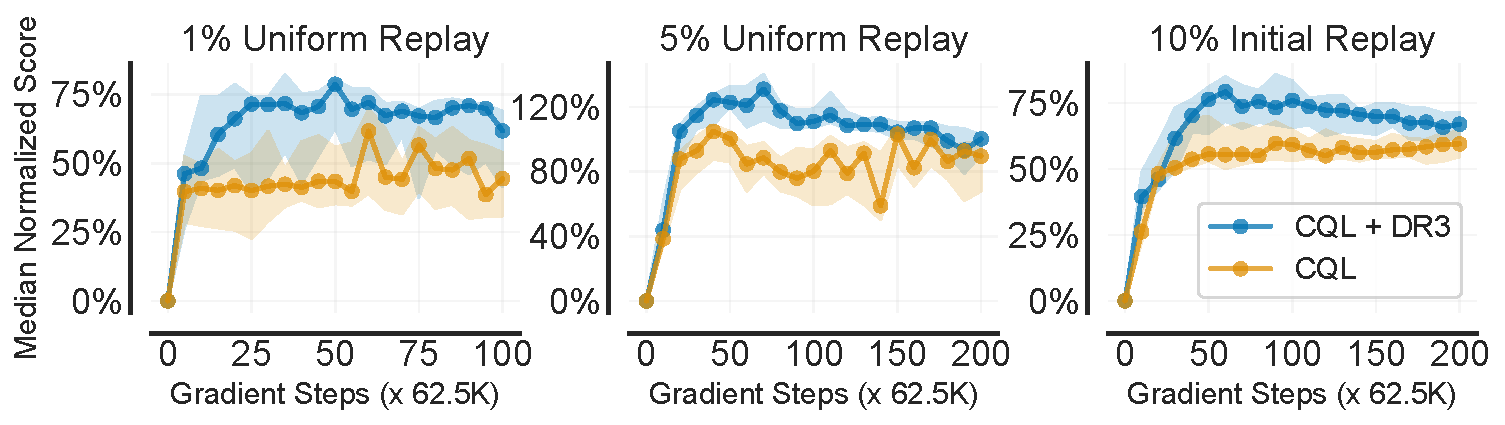
\includegraphics[width=\linewidth]{chapters/dr3/figures/atari_new/Median_cql_penalty.pdf}
%     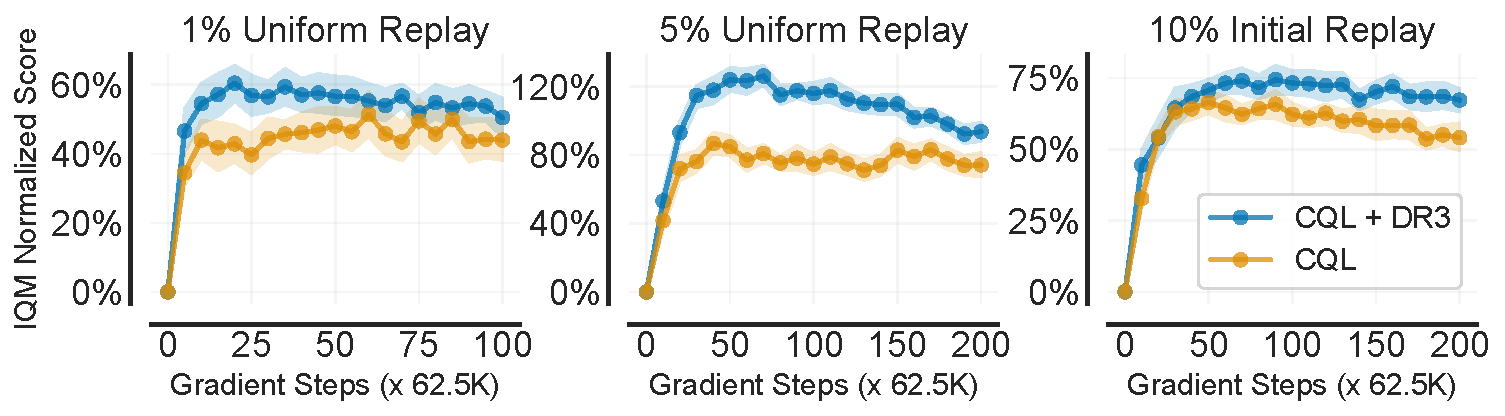
\includegraphics[width=\linewidth]{chapters/dr3/figures/atari_new/IQM_cql_penalty.pdf}
%     % 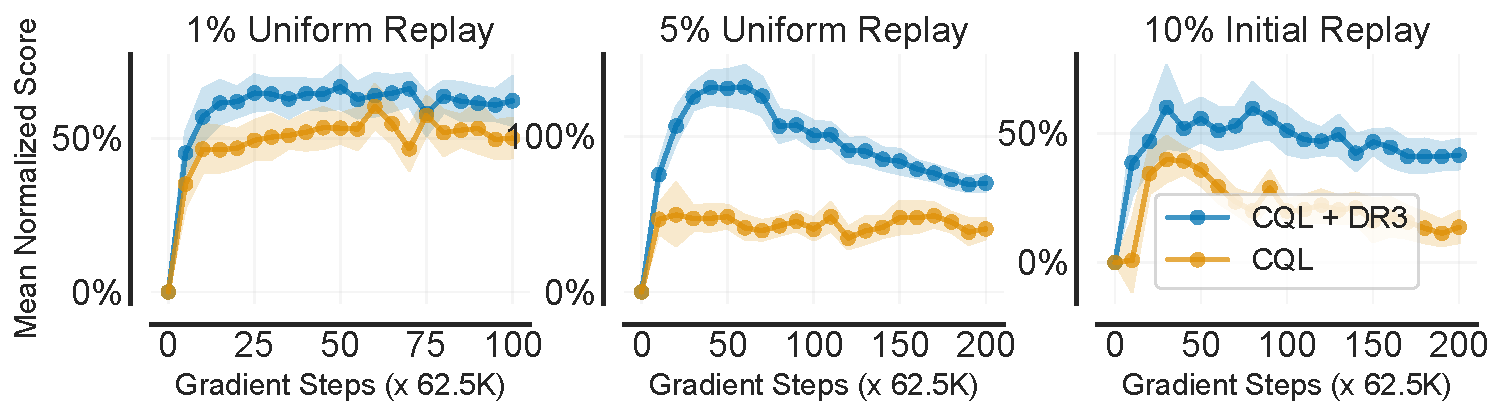
\includegraphics[width=\linewidth]{chapters/dr3/figures/atari_new/Mean_cql_penalty.pdf}
%     % 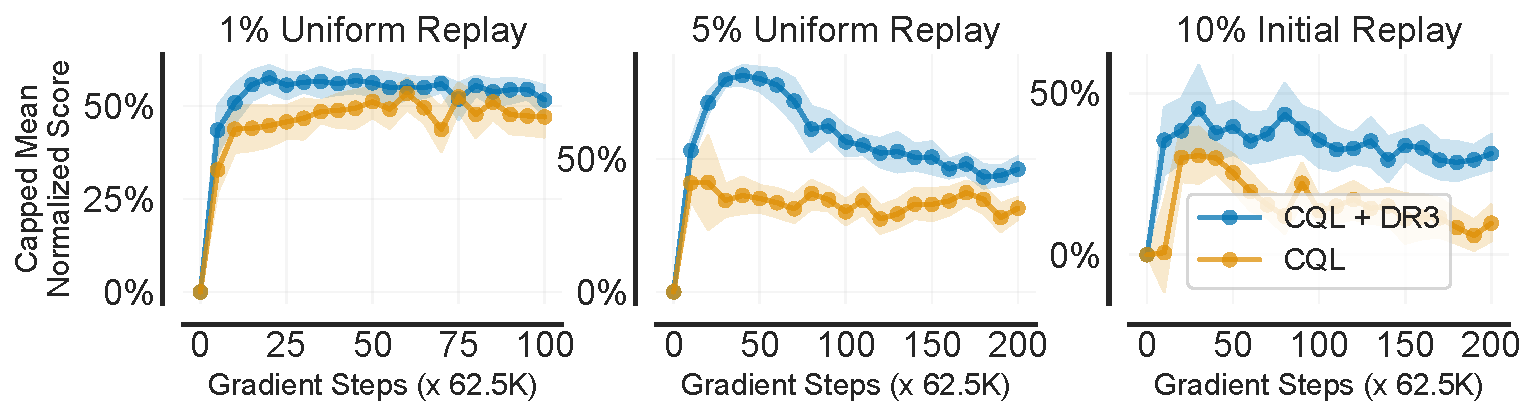
\includegraphics[width=\linewidth]{chapters/dr3/figures/atari_new/Capped_Mean_cql_penalty.pdf}
%     \vspace{-0.65cm}
%     \caption{Behavior Normalized Scores across 17 Atari games. We use Interquartile mean~(IQM).}
%     \label{fig:atari_5_percent}
% \end{figure*}



% \begin{figure}[t]
%     \centering
%     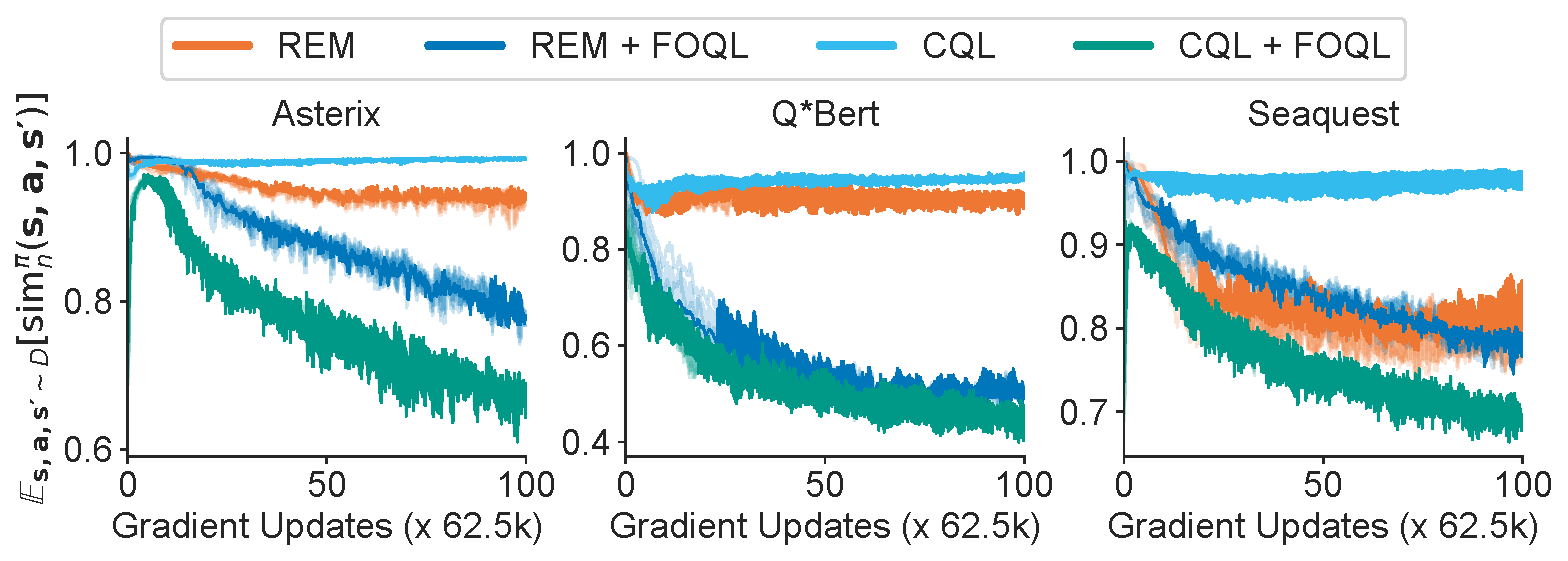
\includegraphics[width=\linewidth]{atari/norm_3_games_cql_rem.pdf}
%     \vspace{-0.65cm}
%     \caption{In addition to minimizing unnormalized similarities~($\simunnorm(\bs, \ba, \bs')$), \drmethodname\ attains much lower normalized similarities as compared to CQL and REM. The results are shown for training with 5\% DQN replay dataset averaged over 5 seeds.}\label{fig:atari_3_cosine}
%     \vspace{-0.5cm}
% \end{figure}


% \begin{figure*}[t]
%     \centering
%     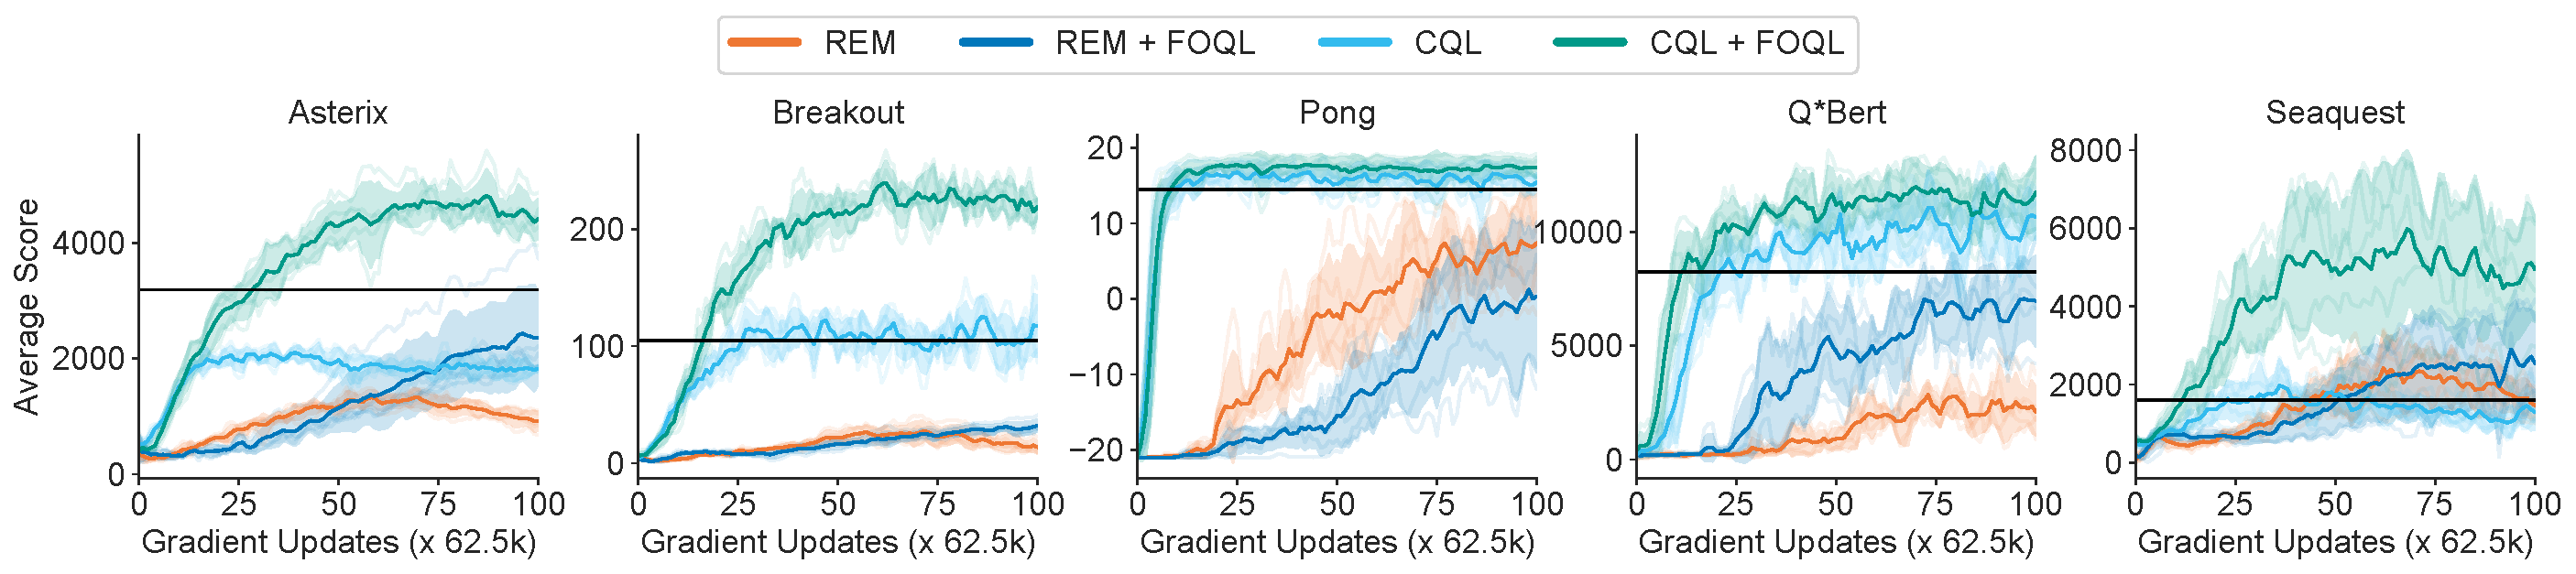
\includegraphics[width=\linewidth]{atari/5_percent_res_100.pdf}
%     \vspace{-0.65cm}
%     \caption{Evaluation performance of offline REM and CQL with and without \drmethodname\ on the 5\% DQN replay dataset~\citep{agarwal2019optimistic}. Note that the data collected during evaluation is not provided to offline agents during training. The horizontal line shows the average performance of the trajectories in entire DQN replay dataset. \drmethodname\ substantially improves the performance of CQL and REM as well as prevents the decay in performance of REM with more gradient updates on \textsc{Seaquest} and \textsc{Asterix}. For \textsc{Pong}, training for longer~(12.5 million updates) results in improved score for REM + \drmethodname\ over REM.}
%     \label{fig:atari_5_percent}
% \end{figure*}


% \begin{table*}[t]
%     \centering
%     \caption{Normalized returns on sub-sampled Atari DQN Replay datasets~\citep{agarwal2019optimistic}. A random policy is provided a normalized score of zero while the average performance of the trajectories in the entire DQN replay dataset is assigned a normalized score of 100. We report results based on 6.5 million gradient updates with batch size of 32 for the 1\% setting and 12.5 million gradient updates for the 5\% and 10\% settings. The individual scores and learning curves for all the 17 games are provided in the Appendix~\ref{app:atari_results}.}
%     \label{tab:cql_res}
%     \vspace{0.2cm}
% \begin{tabular}{cccccc}
% \toprule
% %%AK.1.26: maybe we want to name the average performance as Stability coefficient or something like that but thats a minor point
% \multirow{2}{*}{DQN Replay Setting} & Normalized Score Metric & \multicolumn{2}{c}{Average Performance}   & \multicolumn{2}{c}{Maximum Performance} \\
% & (17 games) & CQL & CQL + \drmethodname & CQL & CQL + \drmethodname \\
% \midrule
% 1\% replay &  Median & 43.3 & \textbf{71.0} & 73.2 & \textbf{96.3} \\
% (uniformly sampled) & Mean & 50.7 & \textbf{60.9} & 74.4 & \textbf{84.6}  \\
% \midrule
% {5\% replay} & Median  & 84.6 & \textbf{104.9} & 127.8 & \textbf{150.7} \\
% (uniformly sampled)  & Mean & 43.3 & \textbf{97.2} &  139.5 & \textbf{189.5}  \\
% \midrule
% {10\% replay} & Median  & 53.4 &  \textbf{69.9} & 73.3 & \textbf{97.2} \\
% (initial exploration data) & Mean & 21.8 & \textbf{49.6} &  79.4 & \textbf{140.0}  \\
% \bottomrule
% \end{tabular}
% \end{table*}

%% Final Performance CQL vs Penalty
% -----DR3+CQL-----
% *****Median*****
% 1% data
% Median 61.8 [41.6 69. ]
% 5% data
% Median 100.2 [ 90.6 102.7]
% 10% data
% Median 67.0 [62.1 71.4]
% *****IQM*****
% 1% data
% IQM 50.5 [44.9 56.1]
% 5% data
% IQM 93.6 [88. 99.]
% 10% data
% IQM 67.3 [63.2 71.4]
% -----CQL-----
% *****Median*****
% 1% data
% Median 44.4 [30.9 54. ]
% 5% data
% Median 89.6 [67.9 98.2]
% 10% data
% Median 59.6 [54.6 64.4]
% *****IQM*****
% 1% data
% IQM 44.0 [38.1 49.8]
% 5% data
% IQM 74.2 [67.3 81.4]
% 10% data
% IQM 54.1 [49.5 59.3]

%% Final performance REM vs REM+penalty
% -----DR3+REM-----
% *****Median*****
% 1% data
% Median 13.1 [10.  18.4]
% 5% data
% Median 72.4 [65.7 81.1]
% 10% data
% Median 72.4 [65.7 81.1]
% *****IQM*****
% 1% data
% IQM 13.4 [11.  16.4]
% 5% data
% IQM 77.2 [71.4 83.9]
% 10% data
% IQM 77.2 [71.4 83.9]
% -----REM-----
% *****Median*****
% 1% data
% Median -0.0 [-0.7  0.1]
% 5% data
% Median 24.9 [14.5 29. ]
% 10% data
% Median 24.9 [14.5 29. ]
% *****IQM*****
% 1% data
% IQM -0.1 [-0.7  0.6]
% 5% data
% IQM 23.5 [19.9 27.3]
% 10% data
% IQM 23.5 [19.9 27.3]


% REM vs REM + penalty Average performance (stability)
% -----DR3+REM-----
% *****Median*****
% 1% data
% Median 11.7
% 5% data
% Median 52.5
% 10% data
% Median 63.9
% *****IQM*****
% 1% data
% IQM 12.4
% 5% data
% IQM 53.5
% 10% data
% IQM 67.8
% -----REM-----
% *****Median*****
% 1% data
% Median 3.1
% 5% data
% Median 18.8
% 10% data
% Median 47.7
% *****IQM*****
% 1% data
% IQM 3.4
% 5% data
% IQM 21.1
% 10% data
% IQM 47.9

% FInal performance (scaled via random scores and CQL is 100\% for IUP comparison):
% Asterix 256.6
% BeamRider 18.6
% Breakout 176.3
% DemonAttack 228.0
% DoubleDunk 133.5
% Enduro 115.2
% IceHockey 51.7
% Jamesbond 310.8
% MsPacman 131.5
% Pong 105.5
% Qbert 114.4
% RoadRunner 100.0
% Seaquest 366.6
% SpaceInvaders 322.8
% WizardOfWor 80.3
% YarsRevenge 75.7
% Zaxxon 485.6



% \begin{table*}[t]
%     \centering
%     \caption{Normalized returns on sub-sampled Atari DQN replay datasets~\citep{agarwal2019optimistic}. The individual scores and learning curves for all the 17 games are provided in the Appendix~\ref{app:atari_results}. When combined with REM, we used a coefficient of $\alpha = 0.001$ to show the robustness of \drmethodname\ across different datasets. \color{red}{Merge the two tables somehow to save space.}}
%     \label{tab:rem_res}
%     \vspace{0.2cm}
% \begin{tabular}{cccccc}
% \toprule
% %%AK.1.26: maybe we want to name the average performance as Stability coefficient or something like that but thats a minor point
% \multirow{2}{*}{DQN Replay Setting} & Normalized Score Metric & \multicolumn{2}{c}{Average Performance}   & \multicolumn{2}{c}{Maximum Performance} \\
% & (17 games) & REM & REM + \drmethodname & REM & REM + \drmethodname \\
% \midrule
% 1\% replay &  Median & 4.7 & \textbf{19.3} & 25.5 & \textbf{42.5} \\
% (uniformly sampled) & Mean & -1.8 & \textbf{47.2} &  72.4 & \textbf{100.2}  \\
% \midrule
% {5\% replay} & Median  & 27.4 & \textbf{58.5} & 88.8 & \textbf{99.8} \\
% (uniformly sampled)  & Mean & 40.9 & \textbf{84.7} &  141.1 & \textbf{165.8}  \\
% \midrule
% {10\% replay} & Median  & 50.7 &  \textbf{68.5} & 107 & \textbf{108.5} \\
% (initial exploration data) & Mean & 63.7 & \textbf{84.4} &  136.5 & \textbf{140.7}  \\
% \bottomrule
% \end{tabular}
% \end{table*}

%% Final Performance CQL vs Penalty
% -----DR3+CQL-----
% *****Median*****
% 1% data
% Median 61.8 [41.6 69. ]
% 5% data
% Median 100.2 [ 90.6 102.7]
% 10% data
% Median 67.0 [62.1 71.4]
% *****IQM*****
% 1% data
% IQM 50.5 [44.9 56.1]
% 5% data
% IQM 93.6 [88. 99.]
% 10% data
% IQM 67.3 [63.2 71.4]
% -----CQL-----
% *****Median*****
% 1% data
% Median 44.4 [30.9 54. ]
% 5% data
% Median 89.6 [67.9 98.2]
% 10% data
% Median 59.6 [54.6 64.4]
% *****IQM*****
% 1% data
% IQM 44.0 [38.1 49.8]
% 5% data
% IQM 74.2 [67.3 81.4]
% 10% data
% IQM 54.1 [49.5 59.3]

% CQL  vs CQL + penalty Average performance (stability)
% -----DR3+CQL-----
% *****Median*****
% 1% data
% Median 63.7
% 5% data
% Median 102.6
% 10% data
% Median 65.2
% *****IQM*****
% 1% data
% IQM 52.6
% 5% data
% IQM 102.4
% 10% data
% IQM 65.2
% -----CQL-----
% *****Median*****
% 1% data
% Median 42.5
% 5% data
% Median 81.4
% 10% data
% Median 52.1
% *****IQM*****
% 1% data
% IQM 42.8
% 5% data
% IQM 72.3
% 10% data
% IQM 56.3


% \begin{table*}[t]
%     \centering
%     \caption{\small{Performance of REM, REM + \drmethodname after 6.5M gradient steps for the 1\% setting and 12.5M gradient steps for the 5\%, 10\% settings. Individual scores for all 17 games are provided in the Appendix~\ref{app:atari_results}.}}
%     \label{tab:rem_res}
%     \vspace{0.2cm}
% \begin{tabular}{cccccc}
% \toprule
% \multirow{2}{*}{\textbf{Data}} & \textbf{Metric} & \multicolumn{2}{c}{\textbf{Last iteration score}}   & \multicolumn{2}{c}{\textbf{Stability score}} \\
% & (17 games) & REM & REM + \drmethodname & REM & REM + \drmethodname \\
% \midrule
% 1\% &  Median & 0.0 & \textbf{13.1} & 3.1 & \textbf{11.7} \\
%  & IQM & -0.1 & \textbf{13.4} & 3.4 & \textbf{12.4}  \\
% \midrule
% 5\% & Median  & 24.9 & \textbf{72.4} & 18.8 & \textbf{52.5} \\
%  & IQM & 23.5 & \textbf{77.2} &  21.1 & \textbf{53.5}  \\
% \midrule
% 10\% & Median & 24.9 &  \textbf{72.4} & 47.7 & \textbf{63.9} \\
%  & IQM & 23.5 & \textbf{77.4} &  47.9 & \textbf{67.8}  \\
% \bottomrule
% \end{tabular}
% \end{table*}



% REM vs REM + penalty Average performance (stability)
% -----DR3+REM-----
% *****Median*****
% 1% data
% Median 11.7
% 5% data
% Median 52.5
% 10% data
% Median 63.9
% *****IQM*****
% 1% data
% IQM 12.4
% 5% data
% IQM 53.5
% 10% data
% IQM 67.8
% -----REM-----
% *****Median*****
% 1% data
% Median 3.1
% 5% data
% Median 18.8
% 10% data
% Median 47.7
% *****IQM*****
% 1% data
% IQM 3.4
% 5% data
% IQM 21.1
% 10% data
% IQM 47.9

%% Final performance REM vs REM+penalty
% -----DR3+REM-----
% *****Median*****
% 1% data
% Median 13.1 [10.  18.4]
% 5% data
% Median 72.4 [65.7 81.1]
% 10% data
% Median 72.4 [65.7 81.1]
% *****IQM*****
% 1% data
% IQM 13.4 [11.  16.4]
% 5% data
% IQM 77.2 [71.4 83.9]
% 10% data
% IQM 77.2 [71.4 83.9]
% -----REM-----
% *****Median*****
% 1% data
% Median -0.0 [-0.7  0.1]
% 5% data
% Median 24.9 [14.5 29. ]
% 10% data
% Median 24.9 [14.5 29. ]
% *****IQM*****
% 1% data
% IQM -0.1 [-0.7  0.6]
% 5% data
% IQM 23.5 [19.9 27.3]
% 10% data
% IQM 23.5 [19.9 27.3]

% \begin{table*}[t]
%     \centering
%     \caption{\small{Performance of REM, REM + \drmethodname after 6.5M gradient steps for the 1\% setting and 12.5M gradient steps for the 5\%, 10\% settings. Individual scores for all 17 games are provided in the Appendix~\ref{app:atari_results}.}}
%     \label{tab:rem_res}
%     \vspace{0.2cm}
% \begin{tabular}{cccccc}
% \toprule
% \multirow{2}{*}{\textbf{Data}} & \textbf{Metric} & \multicolumn{2}{c}{\textbf{Last iteration score}}   & \multicolumn{2}{c}{\textbf{Stability score}} \\
% & (17 games) & REM & REM + \drmethodname & REM & REM + \drmethodname \\
% \midrule
% 1\% &  Median & 0.0 & \textbf{13.1} & 3.1 & \textbf{11.7} \\
%  & IQM & -0.1 & \textbf{13.4} & 3.4 & \textbf{12.4}  \\
% \midrule
% 5\% & Median  & 24.9 & \textbf{72.4} & 18.8 & \textbf{52.5} \\
%  & IQM & 23.5 & \textbf{77.2} &  21.1 & \textbf{53.5}  \\
% \midrule
% 10\% & Median & 24.9 &  \textbf{72.4} & 47.7 & \textbf{63.9} \\
%  & IQM & 23.5 & \textbf{77.4} &  47.9 & \textbf{67.8}  \\
% \bottomrule
% \end{tabular}
% \end{table*}

% \begin{wrapfigure}{r}{0.57\textwidth}
%     \centering
%     \vspace{-5pt}
%     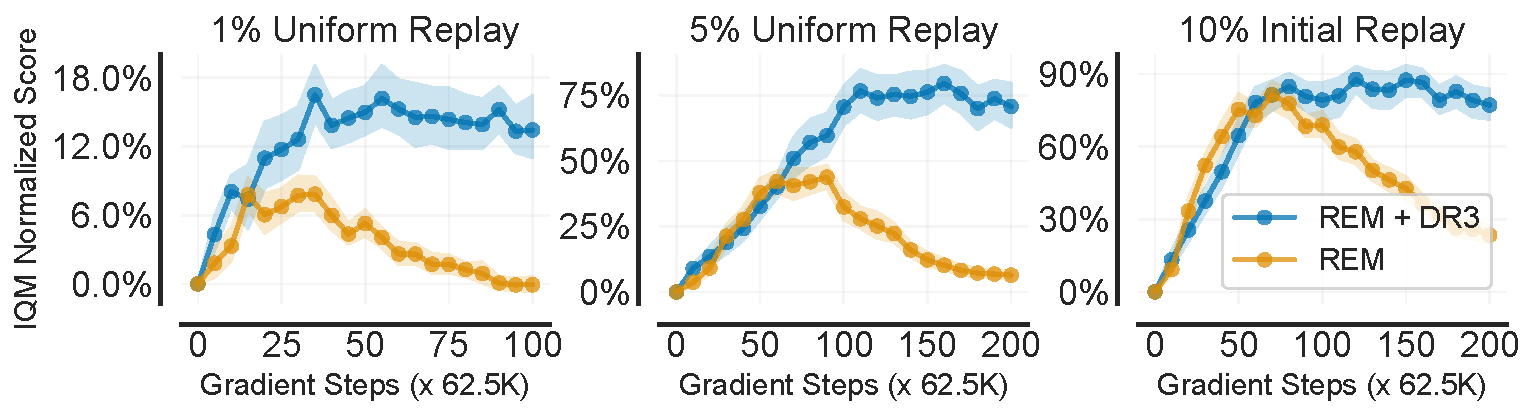
\includegraphics[width=0.99\linewidth]{chapters/dr3/figures/atari_new/IQM_rem_penalty.pdf}
%     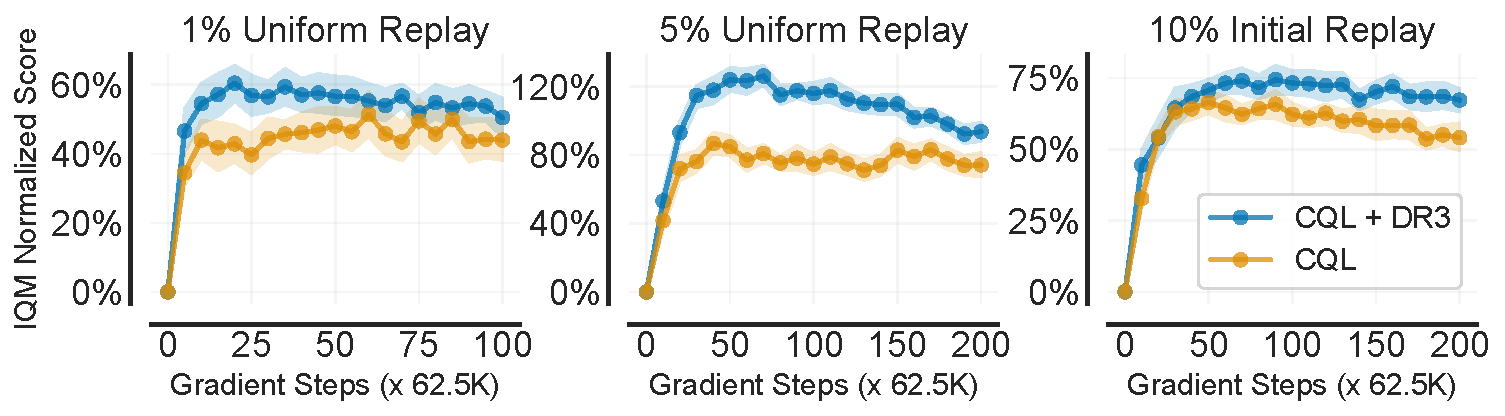
\includegraphics[width=0.99\linewidth]{chapters/dr3/figures/atari_new/IQM_cql_penalty.pdf}
%     \vspace{-0.25in}
%     \caption{\small{\textbf{Average normalized performance across 17 Atari games for REM + \drmethodname\ (top), CQL + \drmethodname\ (bottom)} over the course of training with different datasets. x-axis represents \emph{gradient steps}; no new data is collected. While na\"ive REM suffers from a degradation in performance with more training, REM + \drmethodname\ not only remains generally stable with more training, but also attains higher final performance. CQL + \drmethodname\ attains higher performance than CQL. As recommended by \citet{agarwal2021precipice}, we report interquartile Mean (IQM) with stratified bootstrap 95\% CIs as shaded regions.}}
%     \label{fig:atari_all_combined}
%     \vspace{-0.45cm}
% \end{wrapfigure}
\textbf{{Offline RL on Atari 2600 games.}} We compare \drmethodname\ to prior offline RL methods on a set of offline Atari datasets of varying sizes and quality, akin to \citet{agarwal2019optimistic, kumar2021implicit}. We evaluated on three datasets: \textbf{(1)} 1\% and 5\% samples drawn uniformly at random from DQN replay; \textbf{(2)} a dataset with more suboptimal data consisting of the first 10\% samples observed by an online DQN. Following \citet{agarwal2021precipice}, we report the interquartile mean~(IQM) normalized scores across 17 games over the course of training in Figure~\ref{fig:atari_all_combined} and report the IQM average performance in Table~\ref{tab:cql_res}. Observe that combining \drmethodname\ with modern offline RL methods (CQL, REM) attains the best final and average performance across the 17 Atari games tested on, directly improving upon prior methods
across all the datasets. When \drmethodname\ is used in conjunction with REM, it prevents {severe} unlearning and performance degradation with more training. CQL + \drmethodname\ improves by \textbf{20\%} over CQL on final performance and attains \textbf{25\%} better average performance. {While DR3 is not unequivocally ``stable'', as its performance also degrades relative to the peak it achieves (Figure~\ref{fig:atari_all_combined}), it is more stable relative to base offline RL algorithms.} We also compare \drmethodname\ to the $\mathrm{srank}(\Phi)$ penalty proposed to counter rank collapse~\citep{kumar2021implicit}. Directly taking median normalized score improvements reported by \citet{kumar2021implicit}, CQL + \drmethodname\ improves by over \textbf{2x} (31.5\%) over na\"ive CQL relative to the srank penalty~(14.1\%), indicating DR3's efficacy.
% this $\text{srank}$ penalty only attains a median improvement of 14.1\% over na\"ive CQL, whereas CQL + \drmethodname\ attains a median improvement of \textbf{31.5\%} over CQL. Thus, CQL + \drmethodname\ improves by over \textbf{2x} relative to the srank penalty, indicating DR3's efficacy.
% This indicates that by directly addressing the adverse impacts of implicit regularization, \drmethodname\ can substantially improve upon prior methods that only address its symptoms.  

%Notably, REM performs similar to a random policy in terms of average performance on the 1\%  setting, which is significantly improved by \drmethodname.
%%SL.2.1: I think we can cut this last sentence, and instead focus on the more positive takeaways.

% To evaluate whether the improvements from \drmethodname\ stem from penalizing unnormalized similarities $\simunnorm(\bs, \ba, \bs')$, we also compare \drmethodname\ to penalizing (1) $\simnorm(\bs, \ba, \bs')$, or (2) feature norms~($\|\phi(\bs)\|_2$) on the 5\% dataset on 5 games. The full results, shown in Appendix~\ref{}, confirms that both of these penalties perform substantially worse than \drmethodname, aligned with our theoretical analysis about effectiveness of \drmethodname~(Section~\ref{sec:method_analysis}).

%%SL.2.1: This last phrase is without context. What question is it trying to answer? What is the motivation? Start with a sentence of motivation or a question, then evidence, then answer. Something like: Is [whatever] true? To answer this question, we can [do something]. The full results, shown in [where], indicate [something]. This suggests that [something].
\begin{wrapfigure}{r}{0.42\textwidth}
\small \begin{center}
\vspace{-30pt}
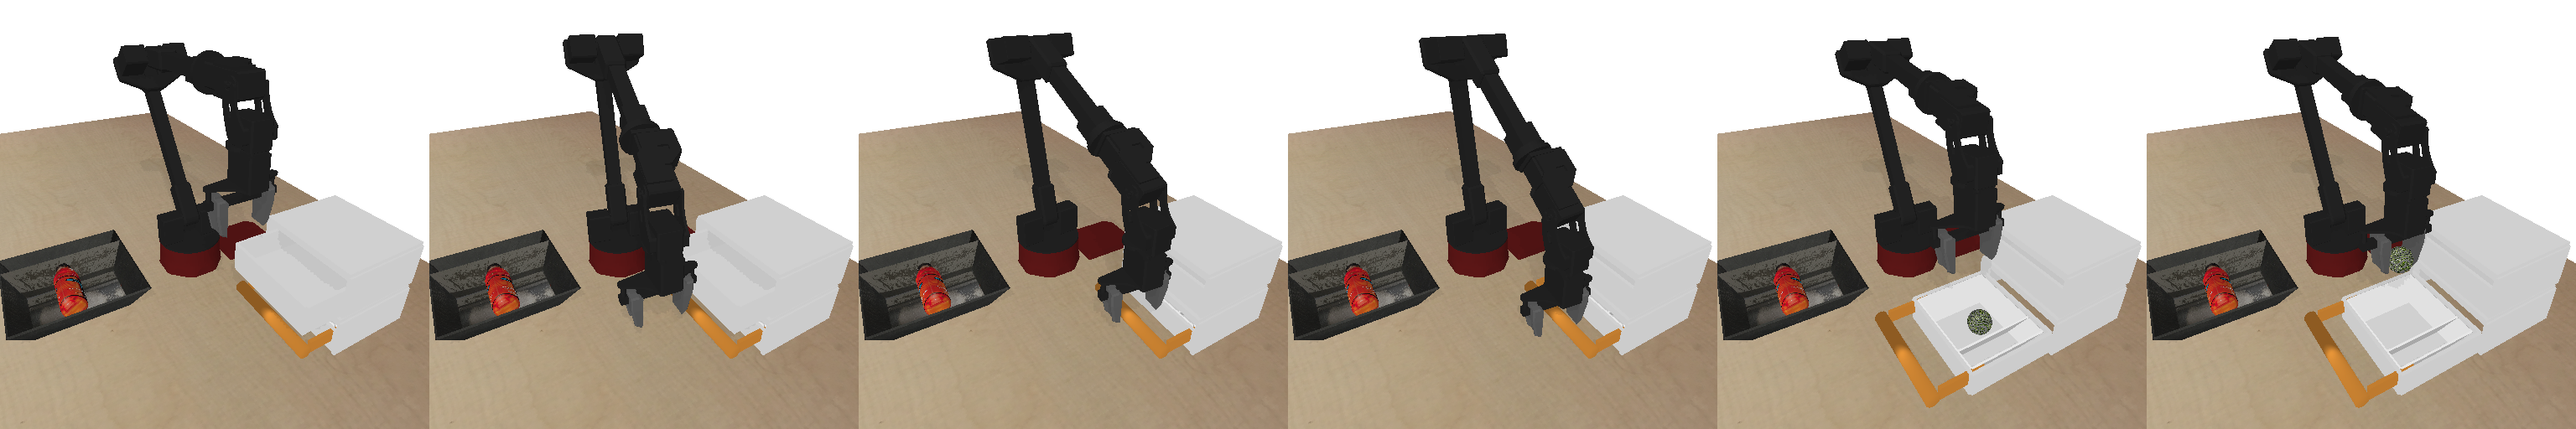
\includegraphics[width=0.99\linewidth]{chapters/dr3/figures/close_open_grasp.png}
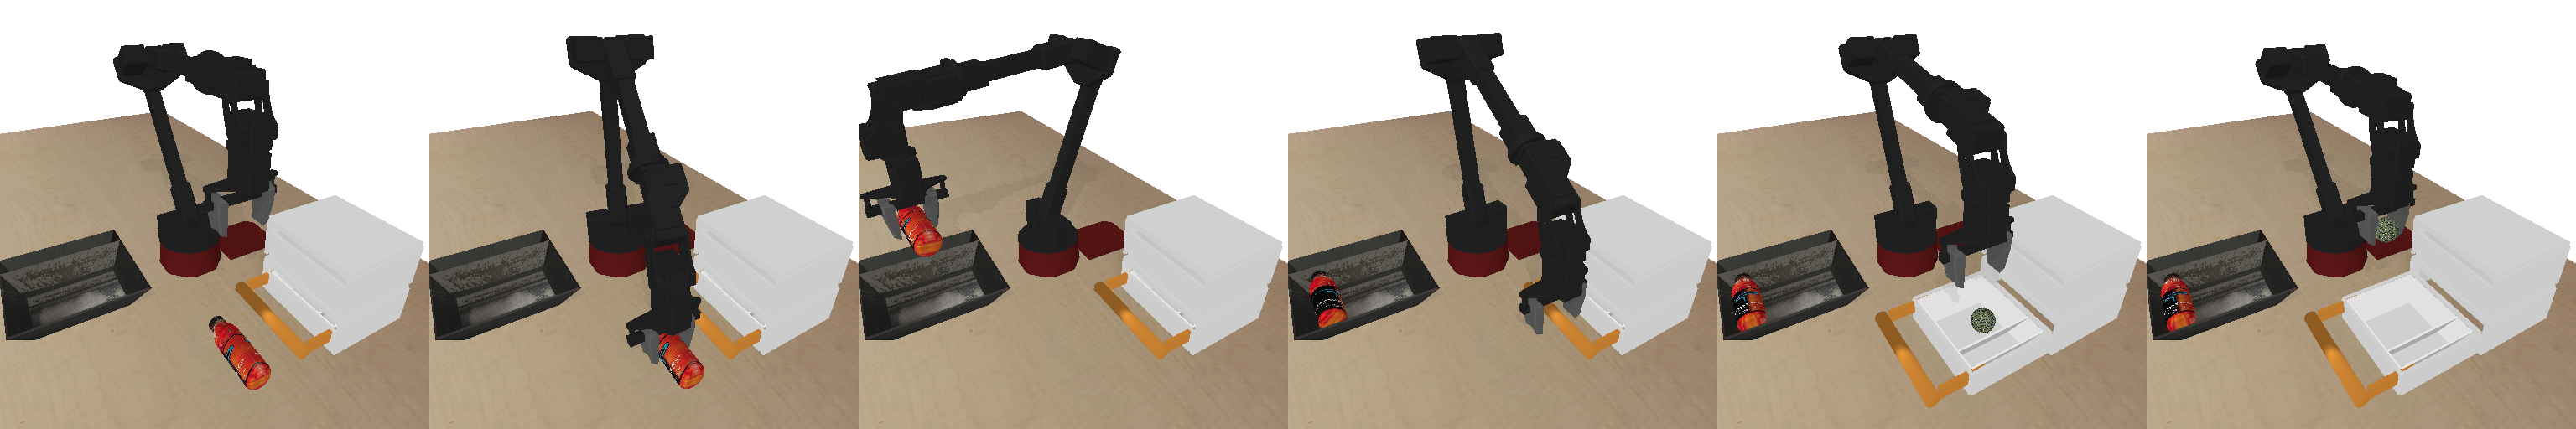
\includegraphics[width=0.99\linewidth]{chapters/dr3/figures/pickplace_open_grasp.png}
\vspace{-20pt}
\end{center}
\end{wrapfigure}
\textbf{{Offline RL on robotic manipulation from}} \textbf{{images.}} Next, we aim to evaluate the efficacy of \drmethodname\ on two image-based robotic manipulation tasks~\citep{singh2020cog}~(visualized on the right) that require composition of skills (e.g., opening a drawer, closing a drawer, picking an obstructive object, placing an object, etc.) over extended horizons using only a sparse 0-1 reward. 
As shown in Figure~\ref{fig:cog_figure}, combining \drmethodname\ with COG improves over COG.

\begin{table}[t]
    \centering
\fontsize{8}{8}\selectfont
    \centering
    \vspace{-0.2cm}
    \caption{\footnotesize{IQM normalized average performance (training stability) across 17 games, with 95\% CIs in parenthesis, after 6.5M gradient steps for the 1\% setting and 12.5M gradient steps for the 5\%, 10\% settings. Individual performances reported in Tables~\ref{tab:cql_dqn_1}-\ref{tab:rem_dqn_10}. \drmethodname\ improves the stability over both CQL and REM.  }}%As recommended by \citet{agarwal2021precipice}, we report IQM with 95\% CIs.}
    \label{tab:cql_res}
    \vspace{-0.1cm}
\begin{tabular}{lcccc}
\toprule
% \multirow{2}{*}{\textbf{Data}}  & \multicolumn{4}{c}{\textbf{Stability performance}} \\
Data & CQL & CQL + \drmethodname & REM & REM + \drmethodname \\
\midrule
1\%   & 43.7~\ss{(39.6, 48.6)} & \textbf{56.9}~\ss{(52.5, 61.2)} & 4.0~\ss{(3.3, 4.8)} & \textbf{16.5}~\ss{(14.5, 18.6)}  \\
\midrule
5\%   &  78.1~\ss{(74.5, 82.4)} & \textbf{105.7}~\ss{(101.9, 110.9)} & 25.9~\ss{(23.4, 28.8)} & \textbf{60.2}~\ss({55.8, 65.1}) \\
\midrule
10\%  & 59.3~\ss{(56.4, 61.9)} & \textbf{65.8}~\ss{(63.3, 68.3)} & 53.3~\ss{(51.4, 55.3)} & \textbf{73.8}~\ss{(69.3, 78)} \\
\bottomrule
\vspace{-0.25in}
\end{tabular}
\end{table}

\begin{figure}[t]
% \vspace{-pt}
\centering
\begin{minipage}{.4\textwidth}
% 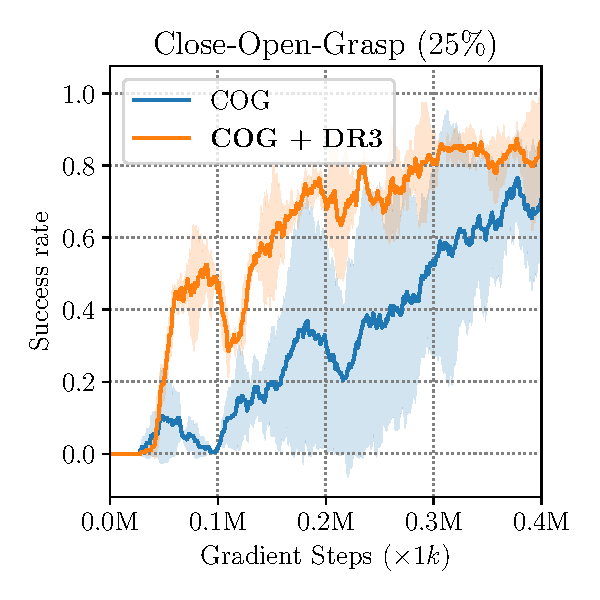
\includegraphics[width=0.49\linewidth]{chapters/dr3/figures/Widow250DoubleDrawerCloseOpenGraspNeutral-v0_cog_vs_dr3_25_v2.pdf}
% 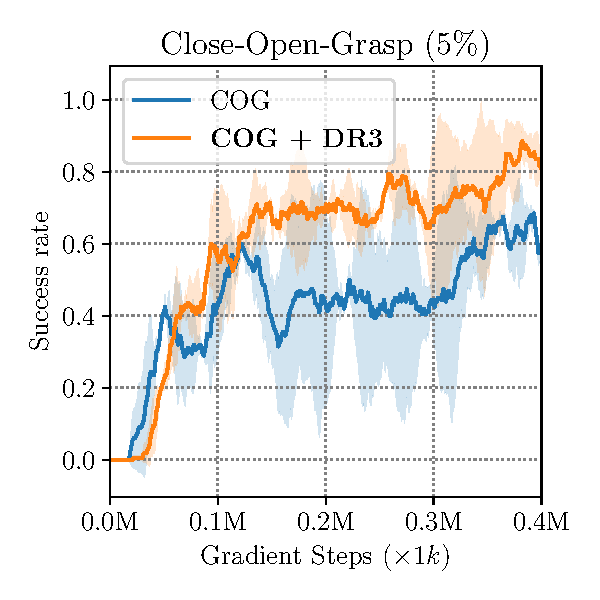
\includegraphics[width=0.49\linewidth]{chapters/dr3/figures/Widow250DoubleDrawerCloseOpenGraspNeutral-v0_cog_vs_dr3_25_v3.pdf}
% 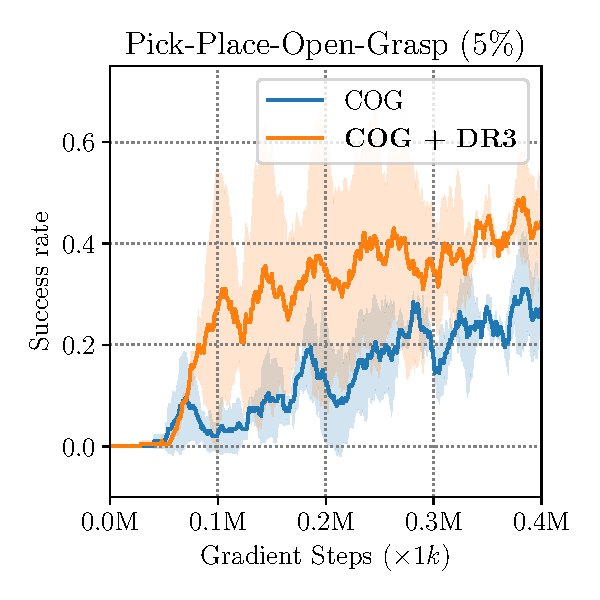
\includegraphics[width=0.49\linewidth]{chapters/dr3/figures/Widow250DoubleDrawerPickPlaceOpenGraspNeutral-v0_cog_vs_dr3_25_v4.pdf}
% 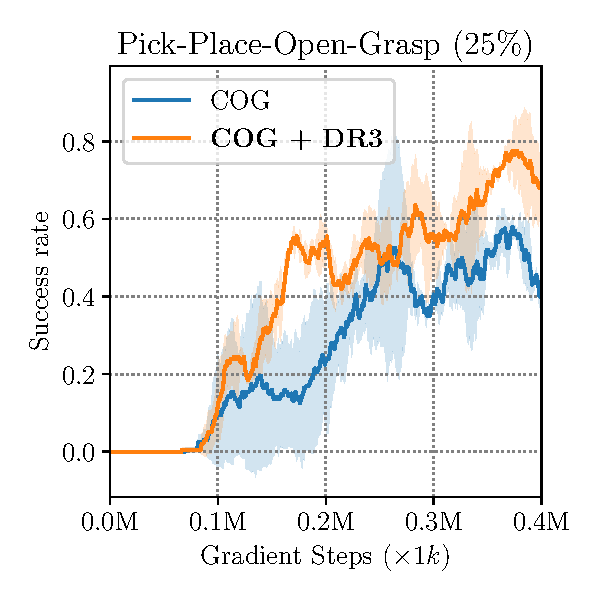
\includegraphics[width=0.49\linewidth]{chapters/dr3/figures/Widow250DoubleDrawerPickPlaceOpenGraspNeutral-v0_cog_vs_dr3_25.pdf}
% \vspace{-10pt}
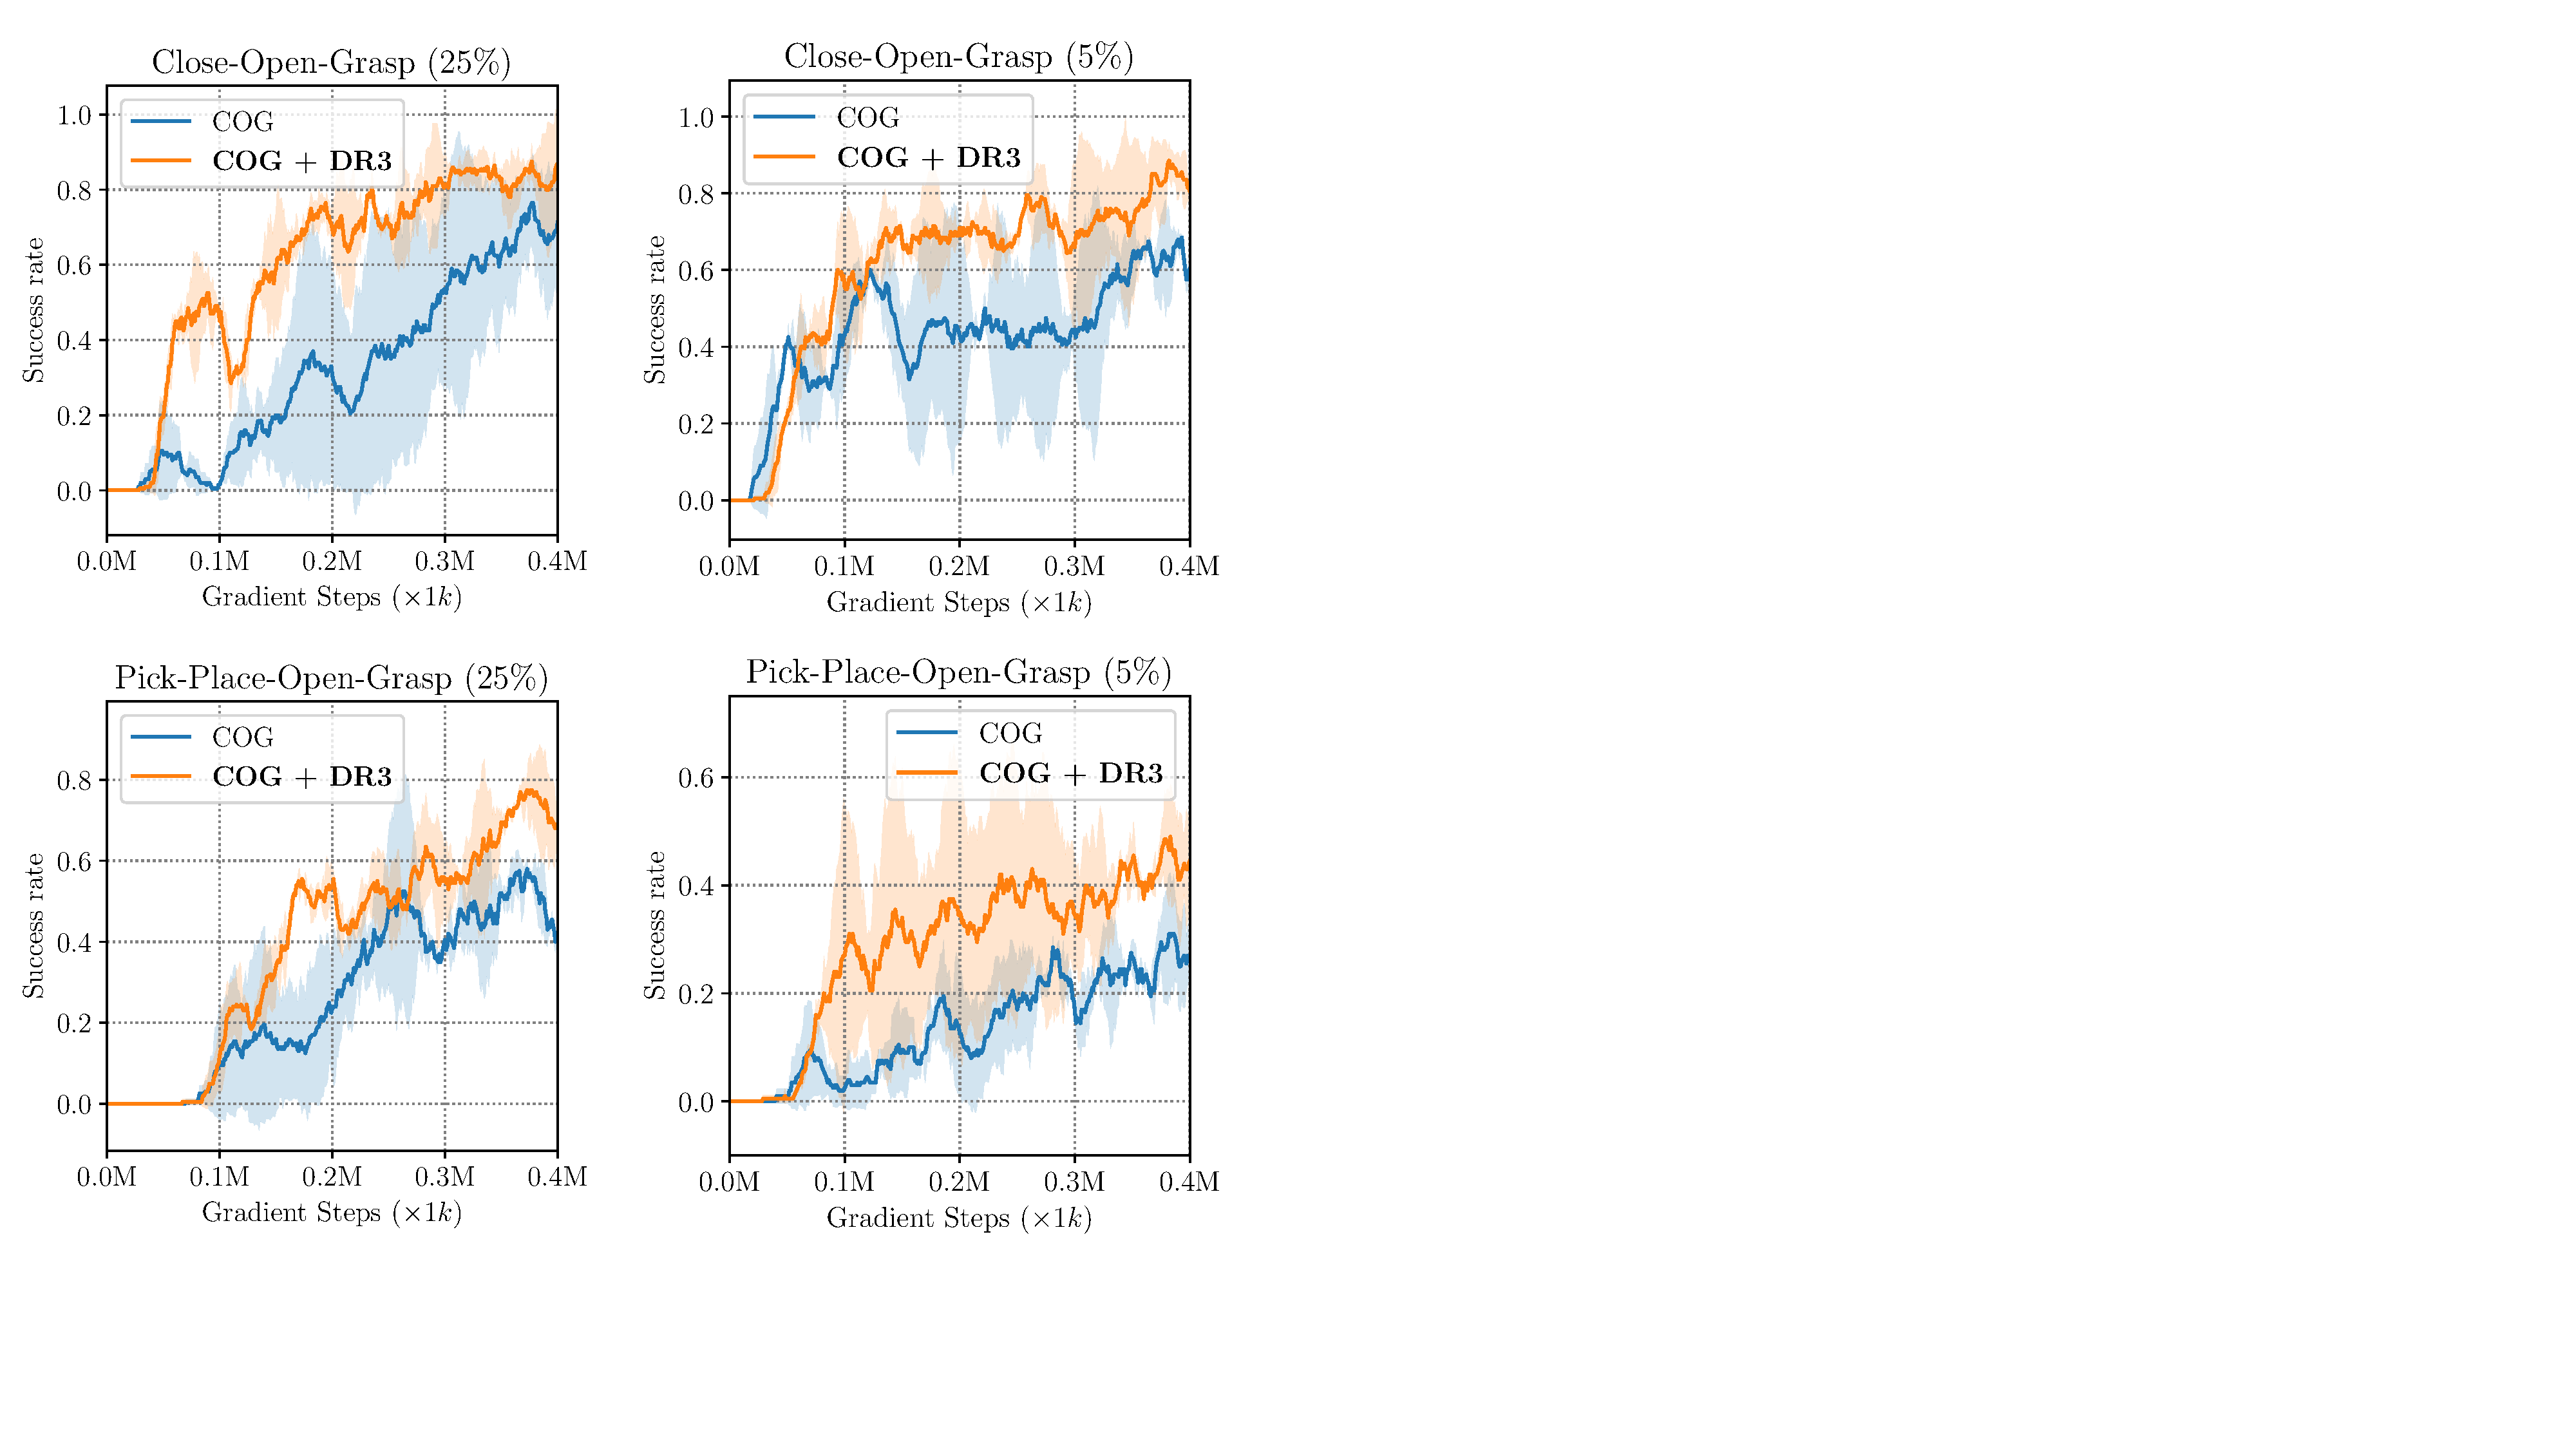
\includegraphics[width=0.96\linewidth]{chapters/dr3/figures/cog_plots.pdf}
\vspace{-0.2cm}
\caption{\footnotesize{\textbf{Performance of \drmethodname\ + COG} on two manipulation tasks using only 5\% and 25\% of the data used by \citet{singh2020cog} to make these more challenging.
COG + \drmethodname\  outperforms COG in training and attains higher average and final performance.}}
\label{fig:cog_figure}
\end{minipage}~~\vline~~
\begin{minipage}{.56\textwidth}
    \centering
    % \vspace{-0.1in}
    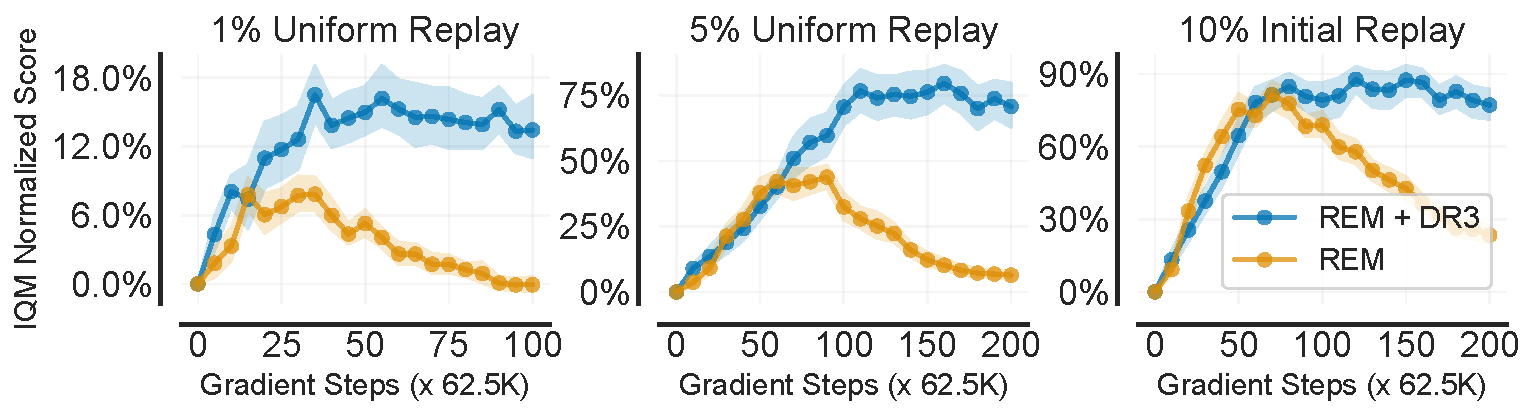
\includegraphics[width=0.99\linewidth]{chapters/dr3/figures/atari_new/IQM_rem_penalty.pdf}
    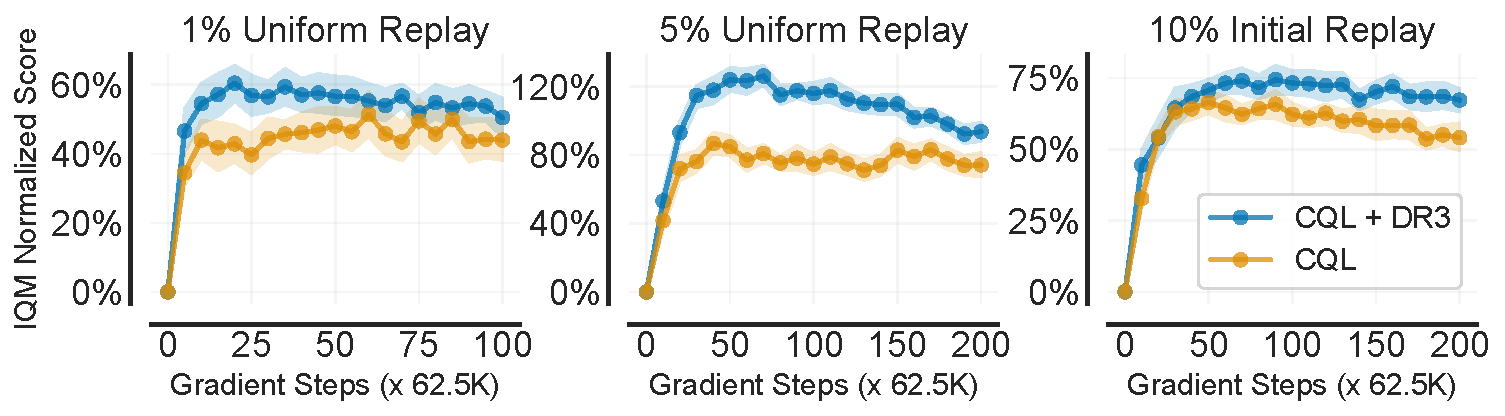
\includegraphics[width=0.99\linewidth]{chapters/dr3/figures/atari_new/IQM_cql_penalty.pdf}
    \vspace{-0.25in}
    \caption{\footnotesize{\textbf{Normalized performance across 17 Atari games for REM + \drmethodname\ (top), CQL + \drmethodname\ (bottom)}. x-axis represents \emph{gradient steps}; no new data is collected. While na\"ive REM suffers from a degradation in performance with more training, REM + \drmethodname\ not only remains generally stable with more training, but also attains higher final performance. CQL + \drmethodname\ attains higher performance than CQL. We report IQM with  95\% stratified bootstrap CIs~\citep{agarwal2021precipice}}.}
    \label{fig:atari_all_combined}
\end{minipage}
\vspace{-0.2cm}
\end{figure}



% \begin{figure}[ht]
% % \vspace{-pt}
% \small \begin{center}
% % \vspace{-10pt}
% % 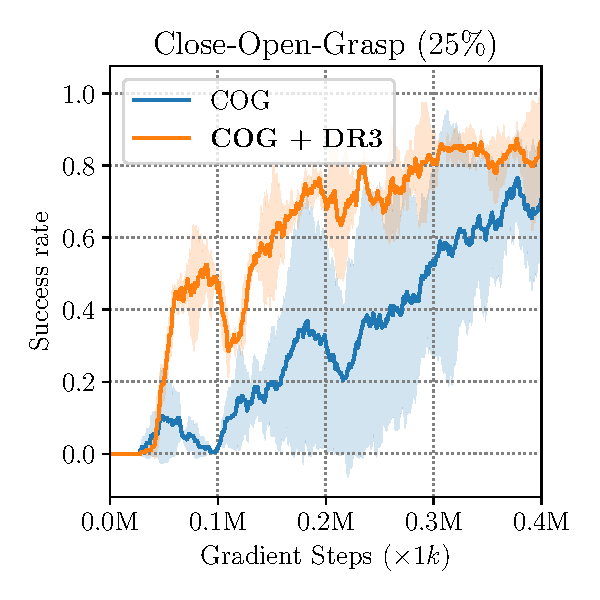
\includegraphics[width=0.49\linewidth]{chapters/dr3/figures/Widow250DoubleDrawerCloseOpenGraspNeutral-v0_cog_vs_dr3_25_v2.pdf}
% % 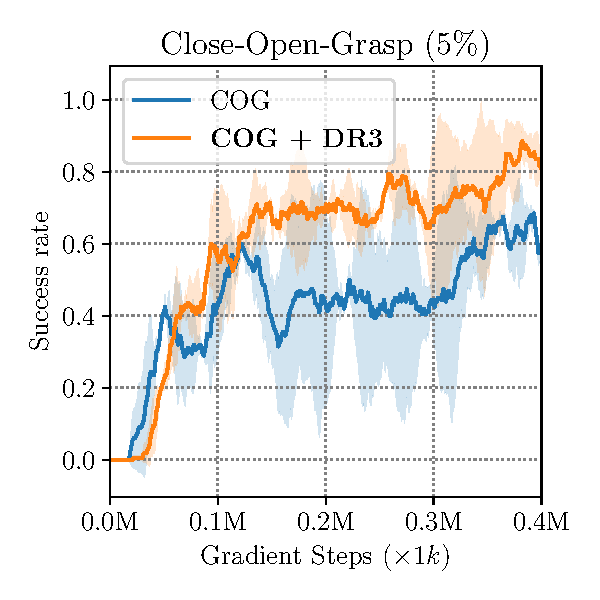
\includegraphics[width=0.49\linewidth]{chapters/dr3/figures/Widow250DoubleDrawerCloseOpenGraspNeutral-v0_cog_vs_dr3_25_v3.pdf}
% % 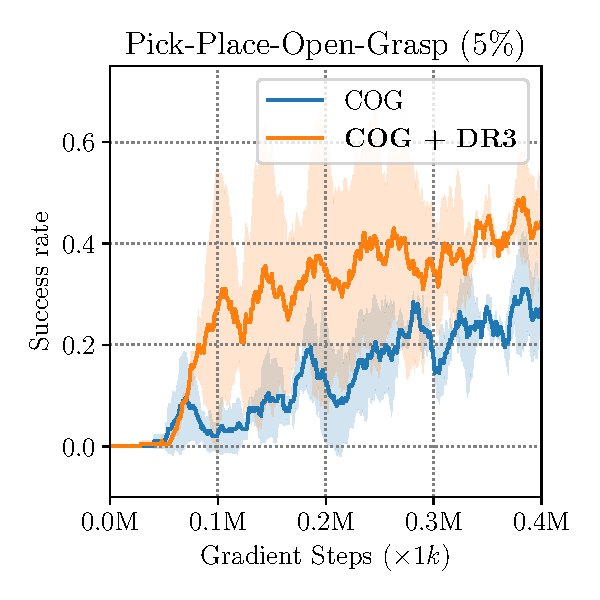
\includegraphics[width=0.49\linewidth]{chapters/dr3/figures/Widow250DoubleDrawerPickPlaceOpenGraspNeutral-v0_cog_vs_dr3_25_v4.pdf}
% % 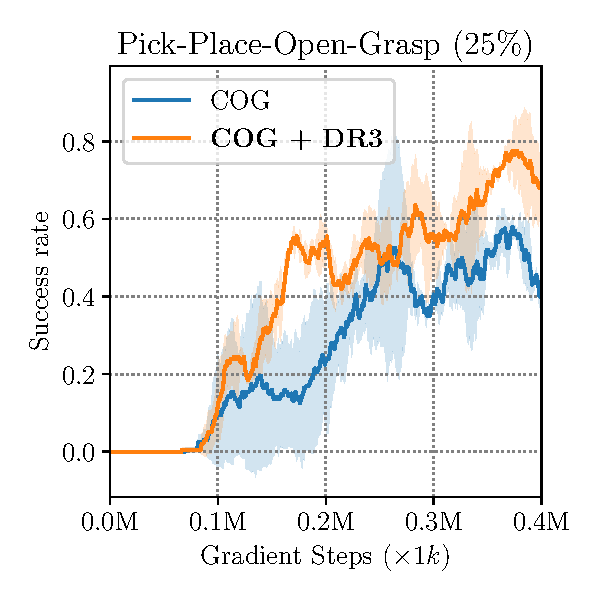
\includegraphics[width=0.49\linewidth]{chapters/dr3/figures/Widow250DoubleDrawerPickPlaceOpenGraspNeutral-v0_cog_vs_dr3_25.pdf}
% 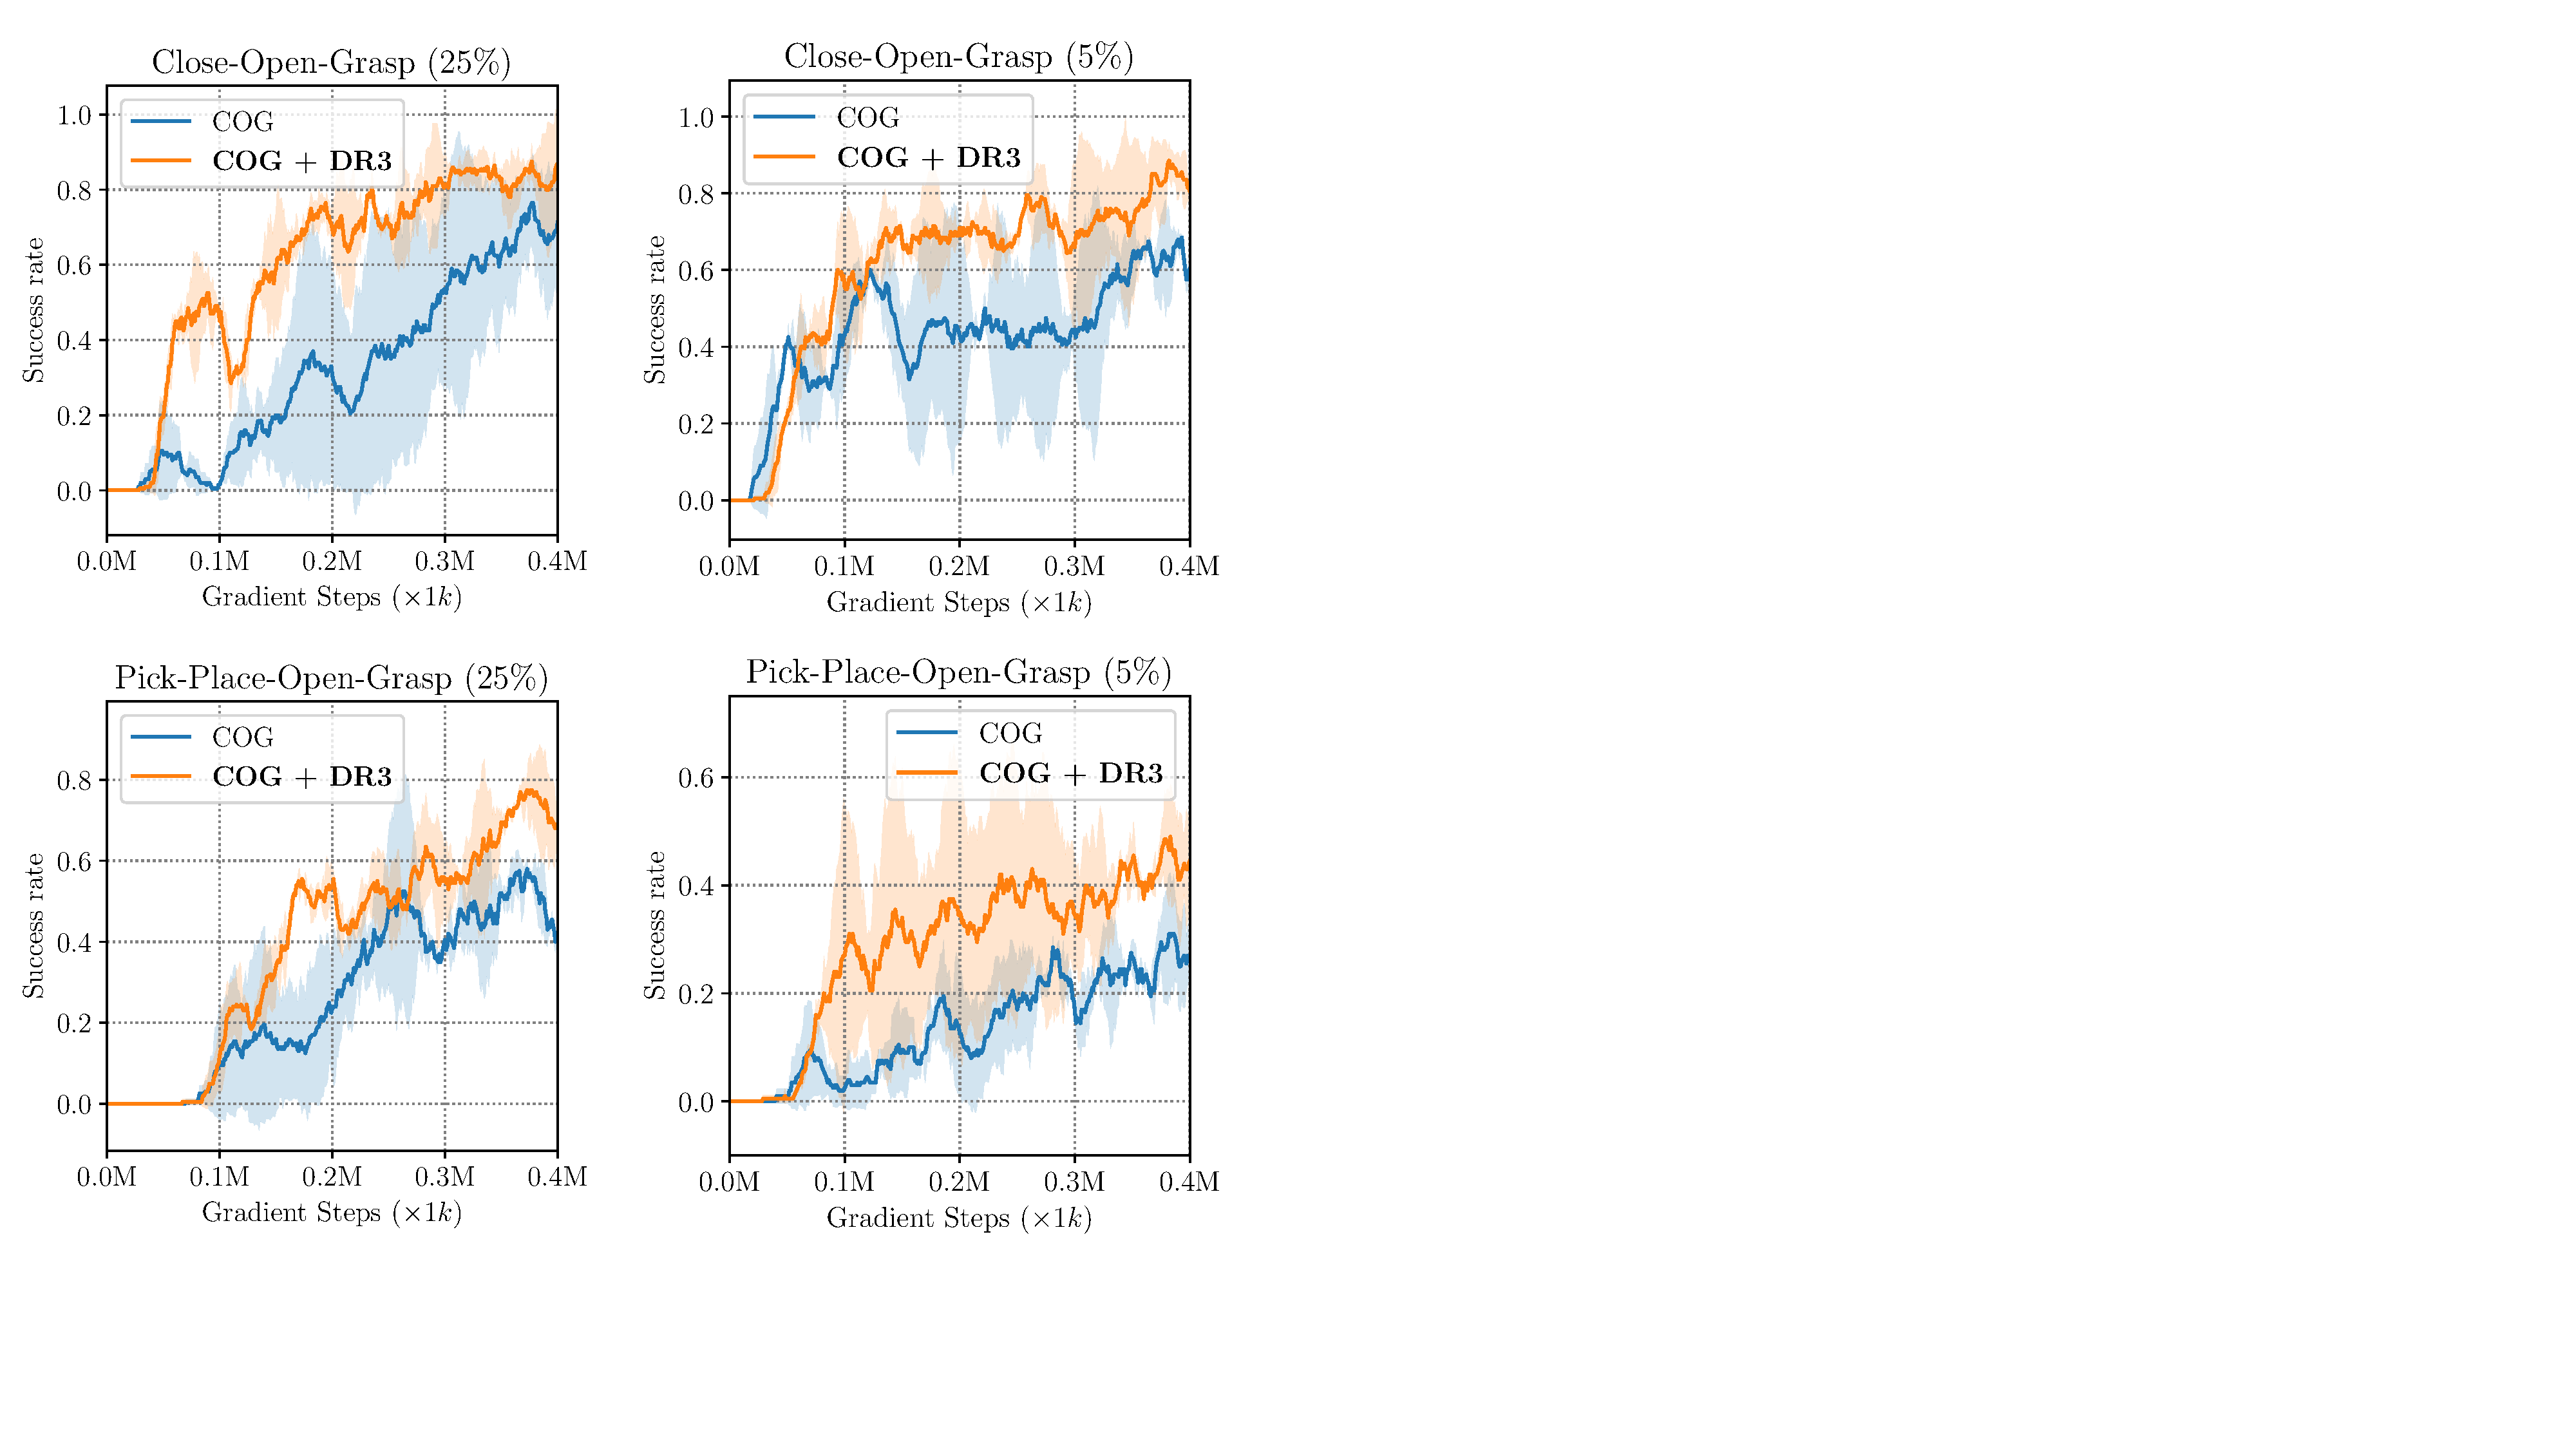
\includegraphics[width=0.5\linewidth]{chapters/dr3/figures/cog_plots.pdf}
% \end{center}
% \vspace{-15pt}
% \caption{\small{\textbf{Performance of \drmethodname\ + COG} on four robotic manipulation settings with different amounts of data. As is visible, COG + \drmethodname\ always outperforms COG and attains higher average and final performance.}}
% \vspace{-5pt}
% \label{fig:cog_figure}
% \end{figure}


%%%%%%%%%%%%%%%%%%%%%%%%% OLD TABLE %%%%%%%%%%%%%%%%%%%%%%%%%%%%%%%
% \begin{figure*}
% % \hline
%     \begin{minipage}{.5\textwidth}
%     \centering
%     \vspace{-0.01in}
%     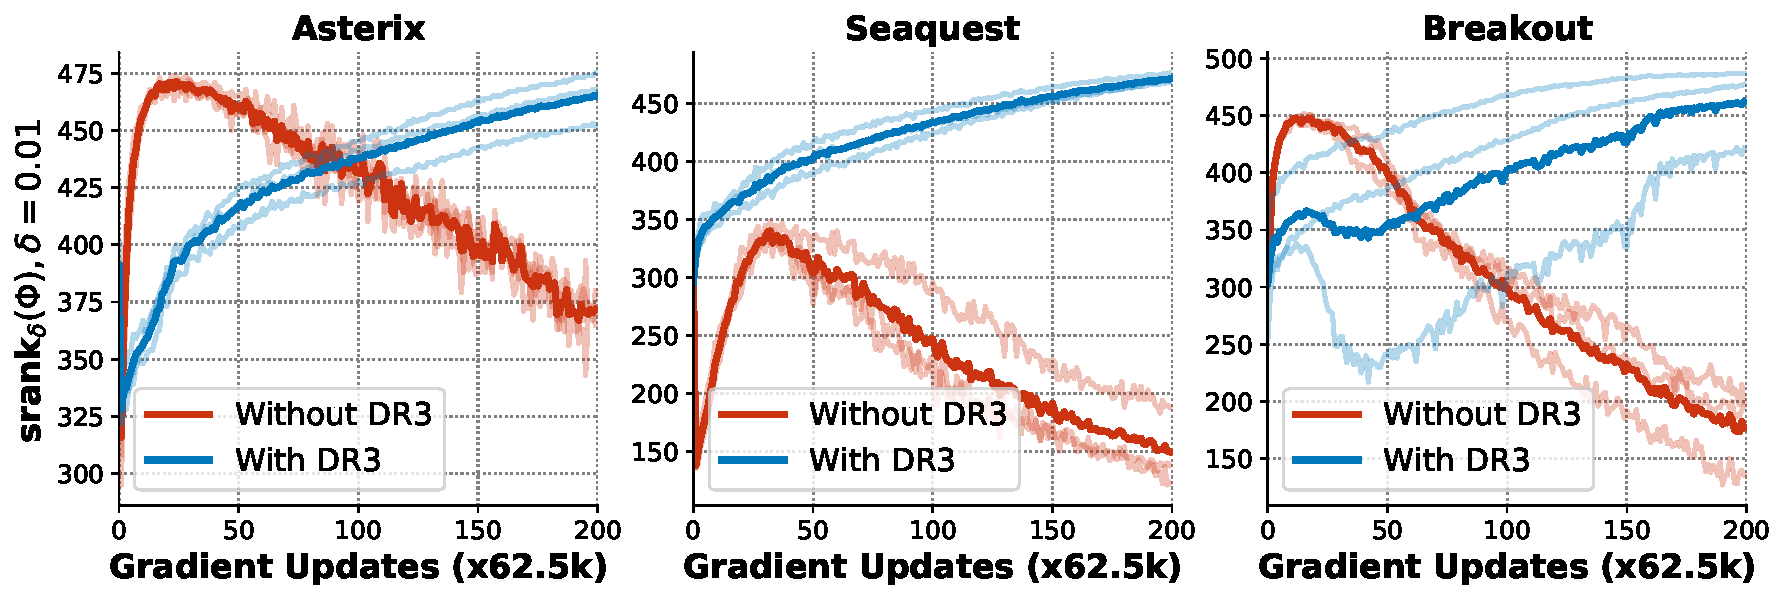
\includegraphics[width=0.99\linewidth]{chapters/dr3/figures/rank_trends_dr3_dqn.pdf}
%     % 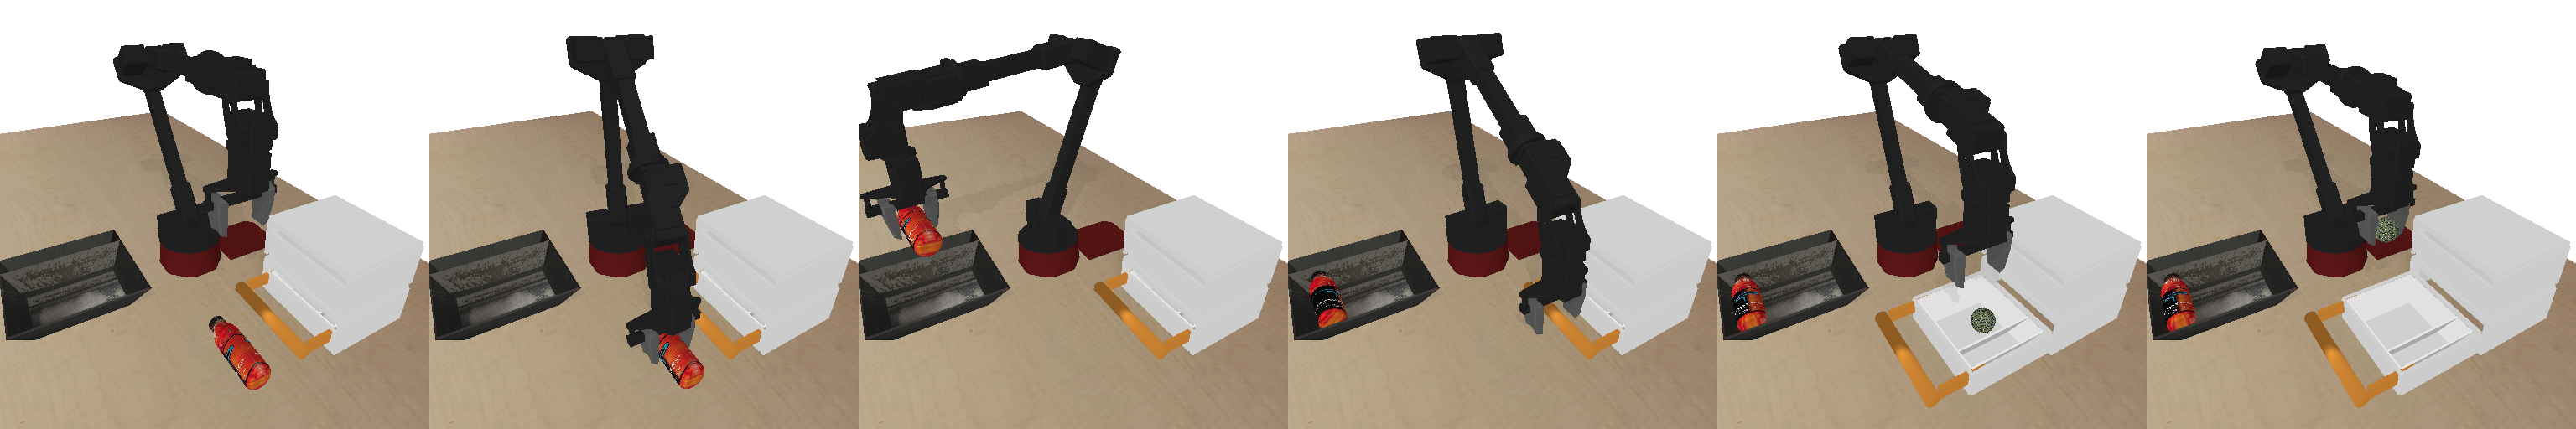
\includegraphics[width=\linewidth]{chapters/dr3/figures/pickplace_open_grasp.png}
%     \vspace{-0.2in}
%     \caption{\footnotesize{{\textbf{Trend of effective rank,} $\mathrm{srank}(\Phi)$ of features $\Phi$ learned by the Q-function when trained with TD error (red, ``Without DR3'') and with TD error + \drmethodname\ (blue, ``With DR3'') on three Atari games using the 5\% dataset. Note that \drmethodname\ alleviates rank collapse observed by \citet{kumar2021implicit}, without explicitly aiming to. Effective rank measures the number of directions with significant singular values~(Appendix~\ref{app:rank_collapse_is_gone}).}}}
%     \label{fig:iup_is_fixed}
%     \vspace{-0.25in}
%     \end{minipage}~~\vline~~
%     \begin{minipage}{.47\textwidth}
%     % \begin{table}[t]
%     % % \vspace{-0.8cm}
%     \vspace{-0.05in}
%     \fontsize{8}{8}\selectfont
%     \centering
%     \captionof{table}{\footnotesize{\textbf{Performance of CQL, CQL + \drmethodname\ after 2M gradient steps with a learning rate of 3e-4} for the Q-function averaged over 4 seeds. This is training for \textbf{6x} longer compared to CQL defaults. Observe that CQL + \drmethodname\ outperforms CQL at 2M steps, indicating is efficacy in inducing stability. %``\texttt{med}'' stands for medium and ``\texttt{lar}'' stands for large.
%     }}
%     \label{tab:cql_d4rl}
%     \vspace{-0.1in}
%     \begin{tabular}{@{}lrr@{}}
%     \toprule
%     {\textbf{D4RL (-v0) Task}} & CQL & CQL + \drmethodname \\
%     \midrule
%     \texttt{kitchen-mixed} & 14.6 $\pm$ 20.5 & \textbf{37.0 $\pm$ 8.0} \\
%     \texttt{kitchen-partial} & 29.6 $\pm$ 19.6 & \textbf{43.5 $\pm$ 1.9}  \\
%     \texttt{kitchen-complete} & 22.3 $\pm$ 17.5 & 24.8 $\pm$ 15.3 \\
%     \midrule
%     \texttt{antmaze-med-diverse} & 0.7 $\pm$ 0.1 & \textbf{0.9 $\pm$ 0.1} \\
%     \texttt{antmaze-med-play} & 0.5 $\pm$ 0.4 & 0.4 $\pm$ 0.3 \\
%     \texttt{antmaze-lar-diverse} & 0.1 $\pm$ 0.0 & \textbf{0.3 $\pm$ 0.16}\\
%     \texttt{antmaze-lar-play} & 0.06 $\pm$ 0.09 & 0.1 $\pm$ 0.01 \\
%     \bottomrule
%     \end{tabular}
%     \vspace{-0.5cm}
%     \end{minipage}
% \end{figure*}
% \hline
% \begin{table}[t]
% % \vspace{-0.8cm}
% \fontsize{8}{8}
% \centering
% \caption{\small{Performance of CQL, CQL + \drmethodname\ after 2M (twice as long as prior work) gradient steps with a learning rate of 3e-4 for the Q-function averaged over 4 seeds. We also find that CQL + \drmethodname\ outperforms CQL at 2M steps, and is comparable to CQL when evaluated at 1M steps, which was the protocol followed originally. ``\texttt{med}'' stands for medium and ``\texttt{lar}'' stands for large.}}
% \label{tab:cql_d4rl}
% \small{
% % \vspace{0.2cm}
% \begin{tabular}{l||r|r}
% \toprule
% {\textbf{D4RL (-v0) Task}} & CQL & \textbf{CQL + \drmethodname} \\
% \midrule
% \texttt{kitchen-mixed} & 14.58 $\pm$ 20.49 & \textbf{37.04 $\pm$ 8.04} \\
% \texttt{kitchen-partial} & 29.63 $\pm$ 19.58 & \textbf{43.54 $\pm$ 1.90}  \\
% \texttt{kitchen-complete} & 22.27 $\pm$ 17.51 & 24.77 $\pm$ 15.3 \\
% \midrule
% \texttt{antmaze-med-diverse} & 0.73 $\pm$ 0.12 & \textbf{0.90 $\pm$ 0.08} \\
% \texttt{antmaze-med-play} & 0.47 $\pm$ 0.36 & 0.36 $\pm$ 0.26 \\
% \texttt{antmaze-lar-diverse} & 0.10 $\pm$ 0.00 & \textbf{0.27 $\pm$ 0.16}\\
% \texttt{antmaze-lar-play} & 0.06 $\pm$ 0.09 & \textbf{0.1 $\pm$ 0.01} \\
% \bottomrule
% \end{tabular}}
% \vspace{-0.5cm}
% \end{table}
%%%%%%%%%%%%%%%%%%%%%%%%%%%%%%%%%%%%%%%%%%%%%%%%%%%%%%%%%%%%%%%%%%%%%%%%%%%%%%%%

% \textbf{{Offline RL on D4RL tasks.}} Finally, we evaluate DR3 in conjunction with CQL on the antmaze and kitchen domains in D4RL~\citep{fu2020d4rl}. To assess if \drmethodname\ is stable and able to prevent unlearning that eventually appears in CQL, we trained CQL+\drmethodname\ for \textbf{6x} longer: 2M steps with 3x higher learning rate. %This is different from prior works~\citep{kumar2020conservative} that report performance at the end of 1M steps.
% Observe in Table~\ref{tab:cql_d4rl}, that CQL + \drmethodname\ outperforms CQL ({statistical significance shown in Appendix~\ref{app:significance}}). {We show that CQL + DR3 also outperforms base CQL in terms of performance and stability on MuJoCo tasks previously studied in \citet{kumar2021implicit} in Appendix~\ref{app:mujoco}.} 
% %%SL.10.2: I don't see how "indicating the ability to train for more gradient steps" follows from these results -- where is the evidence for this? did you change the number of steps? Also, this section appears to violate what you said before about reporting stability: you said that stability = average over iterations, but here you are not reporting it. If this is how it is, then maybe revise the beginning of the experiments section, which makes a really big deal out of this stability metric. I *think* what you mean is that training for 2M steps evaluates stability better than 1M steps, but critical readers will just say you cherry-picked the number of steps that makes your method look good.
% Further, we also compare the effect of adding \drmethodname\ to BRAC~\citep{wu2019behavior}.
% %%SL.10.2: such as BRAC, or just BRAC?
% \drmethodname\ applied on BRAC improves final median normalized score performance by \textbf{13.8}  and stability by \textbf{8.1} across 15 MuJoCo tasks. Numbers for BRAC can be found in Table~\ref{tab:brac}.
% %%AK: unfortunately this table is in the Appendix.

\iffalse

\textbf{{Offline RL on D4RL tasks.}} Finally, we evaluate DR3 in conjunction with CQL on the antmaze-v2 domain in D4RL~\citep{fu2020d4rl}. To assess if \drmethodname\ is stable and able to prevent unlearning that eventually appears in CQL, we trained CQL+\drmethodname\ for \textbf{9x} longer: 2M and 3M steps with 3x higher learning rate. This is different from prior works~\citep{fu2020d4rl} that report performance at the end of 1M steps.
Observe in Table~\ref{tab:cql_d4rl}, that CQL + \drmethodname\ outperforms CQL ({statistical significance shown in Appendix~\ref{app:significance}}), indicating that DR3 significantly improves CQL. We also evalute DR3 on kitchen domains in D4RL in Appendix~\ref{app:significance}, where we also find that DR3 improves CQL. Finally, we also compare CQL+DR3 and CQL in terms of performance and stability on MuJoCo tasks previously studied in \citet{kumar2021implicit} in Appendix~\ref{app:mujoco}. These tasks are constructed by uniformly subsampling transitions from the full-replay-v2 MuJoCo datasets in D4RL and are much harder than the typical Gym-MuJoCo tasks from \citet{fu2020d4rl} because succeeding on these tasks critically relies on estimating accurate Q-values for out-of-sample actions and all actions at certain states are out-of-sample. As shown in Appendix~\ref{app:mujoco}, CQL+DR3 is significantly more stable, and does not unlearn with more training, unlike CQL whose performance degrades very quickly. We also evaluate DR3 in conjunction with BRAC~\citep{wu2019behavior}, a policy constraint method, and find that BRAC+DR3 improves over BRAC in \textbf{13.8} median normalized performance (Table~\ref{tab:brac}).
% \textbf{These results} indicate that \drmethodname\ is a versatile explicit regularizer that improves performance and stability of a wide range of offline RL methods. 

\begin{table*}[t]
    % \begin{table}[t]
    % % \vspace{-0.8cm}
    % \vspace{-0.25cm}
    \fontsize{8}{8}\selectfont
    \centering
    \captionof{table}{\footnotesize{\textbf{Performance of CQL, CQL + \drmethodname\ after 2M and 3M gradient steps with a learning rate of 3e-4} for the Q-function averaged over 3 seeds. This is training for \textbf{6x} and \textbf{9x} longer compared to CQL defaults. Observe that CQL + \drmethodname\ outperforms CQL at 2M and 3M steps, indicating is efficacy in preventing unlearning. We present the statistical significance of these results in Appendix~\ref{app:significance}.}}
    \label{tab:cql_d4rl}
    \vspace{-0.1in}
    \begin{tabular}{@{}l|rr||rr@{}}
    \toprule
    {\textbf{D4RL Task}} & \textbf{CQL} (2M) & \textbf{CQL + \drmethodname} (2M) & \textbf{CQL} (3M) & \textbf{CQL + \drmethodname} (3M)  \\
    \midrule
    % \texttt{kitchen-mixed} & 14.6 $\pm$ 20.5 & \textbf{37.0 $\pm$ 8.0} \\
    % \texttt{kitchen-partial} & 29.6 $\pm$ 19.6 & \textbf{43.5 $\pm$ 1.9}  \\
    % \texttt{kitchen-complete} & 22.3 $\pm$ 17.5 & 24.8 $\pm$ 15.3 \\
    % \midrule
    \texttt{antmaze-umaze-v2} & 84.00 $\pm$ 2.67 & 85.33 $\pm$ 4.16 & 87.00 $\pm$ 1.73 & 90.00 $\pm$ 4.00 \\ 
    \texttt{antmaze-umaze-diverse-v2} & 45.67 $\pm$ 8.50 & 40.67 $\pm$ 11.84 & 36.33 $\pm$ 7.09 & \textbf{52.00 $\pm$ 11.26} \\
    \texttt{antmaze-medium-play-v2} & 24.00 $\pm$ 28.16 & \textbf{73.00 $\pm$ 4.00} & 16.00 $\pm$ 26.85 & \textbf{71.33 $\pm$ 1.52} \\
    \texttt{antmaze-medium-diverse-v2} & 32.67 $\pm$ 9.29 & \textbf{67.00 $\pm$ 2.00} & 48.33 $\pm$ 6.11 & \textbf{61.67 $\pm$ 3.21} \\
    \texttt{antmaze-large-play-v2} & 3.33 $\pm$ 2.51 & \textbf{28.00 $\pm$ 4.35} & 0.33 $\pm$ 0.57 & \textbf{26.33 $\pm$ 11.93} \\
    \texttt{antmaze-large-diverse-v2} & 1.33 $\pm$ 2.30 & \textbf{25.67 $\pm$ 0.57} & 0.00 $\pm$ 0.00 & \textbf{28.33 $\pm$ 1.52} \\
    \bottomrule
    \end{tabular}
    \vspace{-0.4cm}
    \end{table*}

\fi


% \begin{wrapfigure}{r}{0.57\textwidth}
% \small \begin{center}
% \vspace{-0.3in}
% 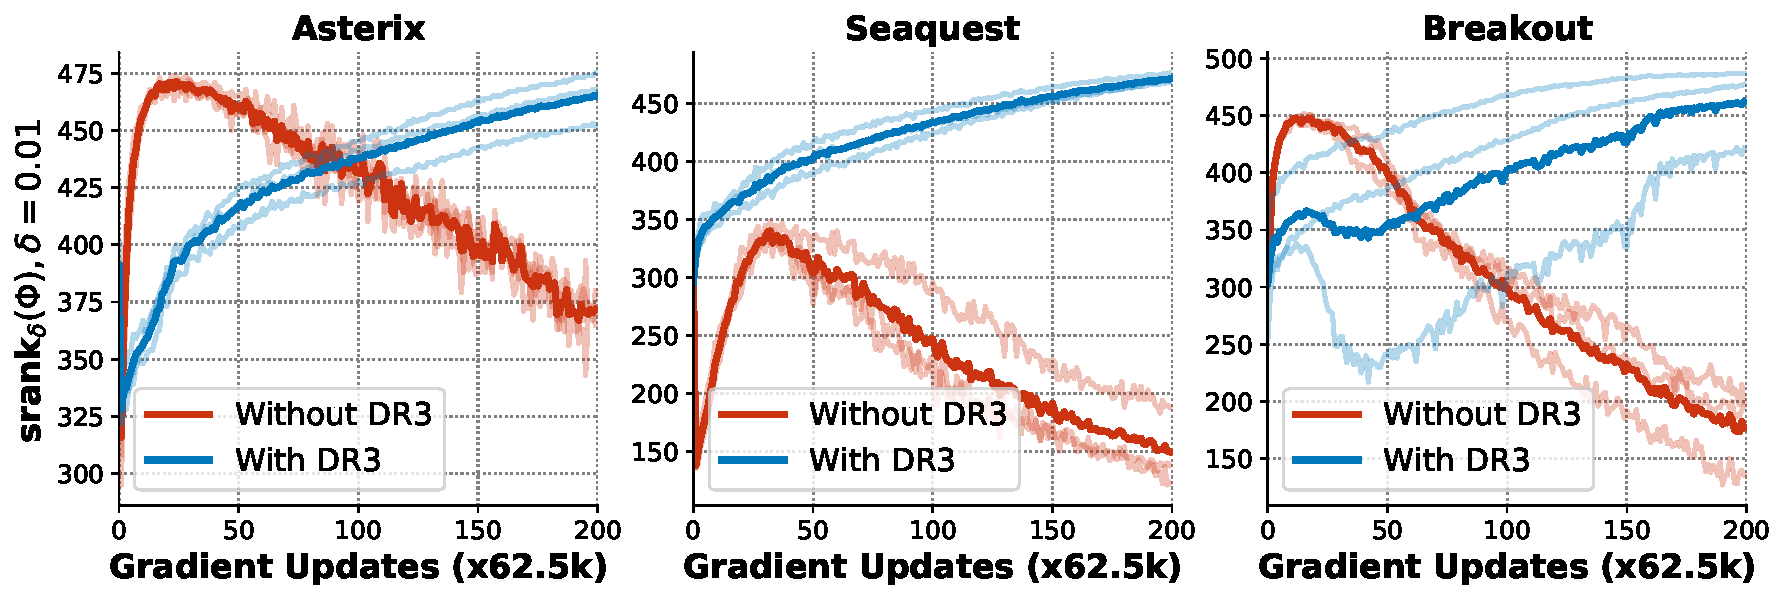
\includegraphics[width=0.99\linewidth]{chapters/dr3/figures/rank_trends_dr3_dqn.pdf}
% % 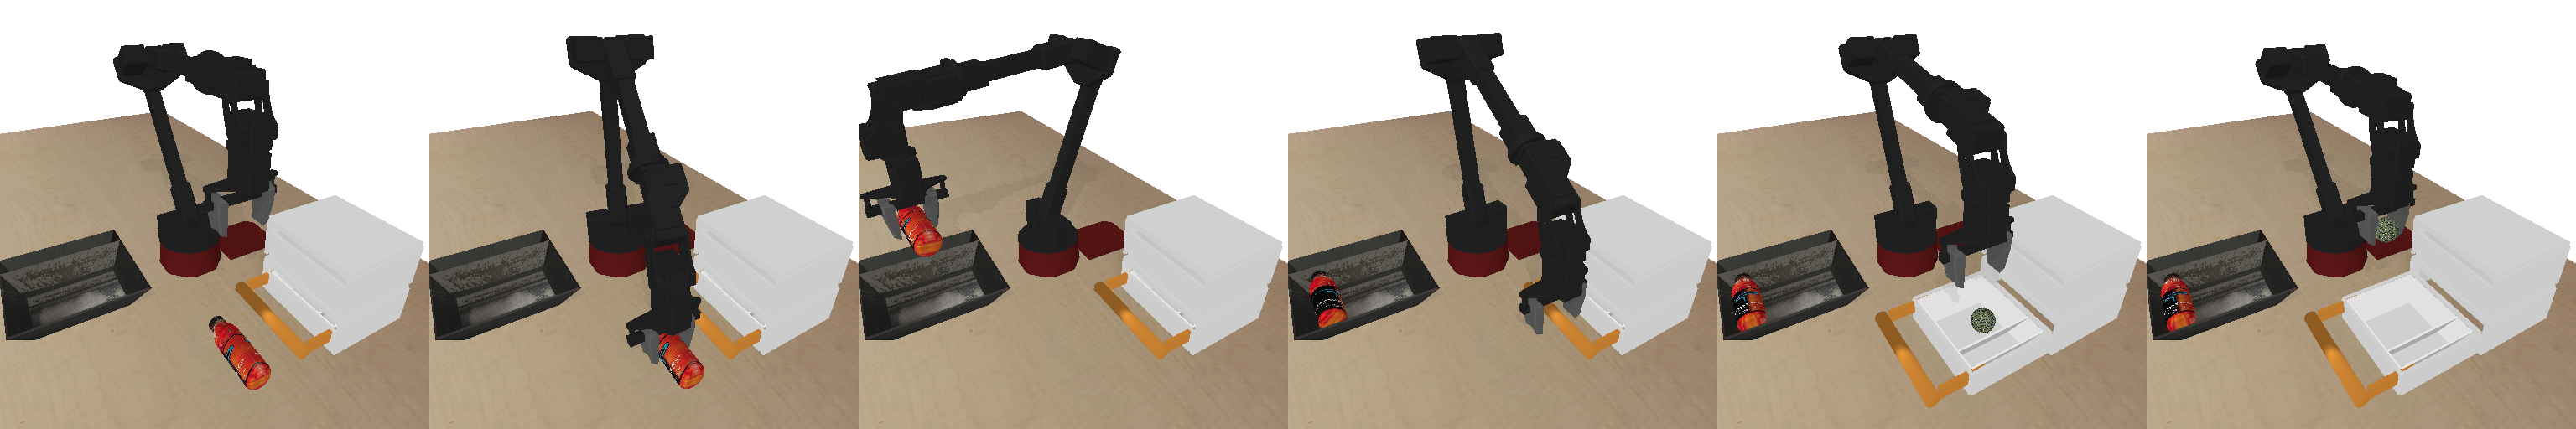
\includegraphics[width=\linewidth]{chapters/dr3/figures/pickplace_open_grasp.png}
% \vspace{-0.1in}
% \caption{\small{{\textbf{Trend of effective rank,} $\mathrm{srank}(\Phi)$ of features $\Phi$ learned by the Q-function when trained with TD error (red, ``Without DR3'') and with TD error + \drmethodname\ (blue, ``With DR3'') on three Atari games using the 5\% dataset. Note that \drmethodname\ clearly alleviates rank collapse, without explicitly aiming to.}}}
% \label{fig:iup_is_fixed}
% \end{center}
% \vspace{-0.25in}
% \end{wrapfigure}
\begin{figure}[h]
    \centering
    \vspace{-0.1in}
    \includegraphics[width=0.8\linewidth]{chapters/dr3/figures/rank\_trends\_dr3\_dqn.pdf}
    % 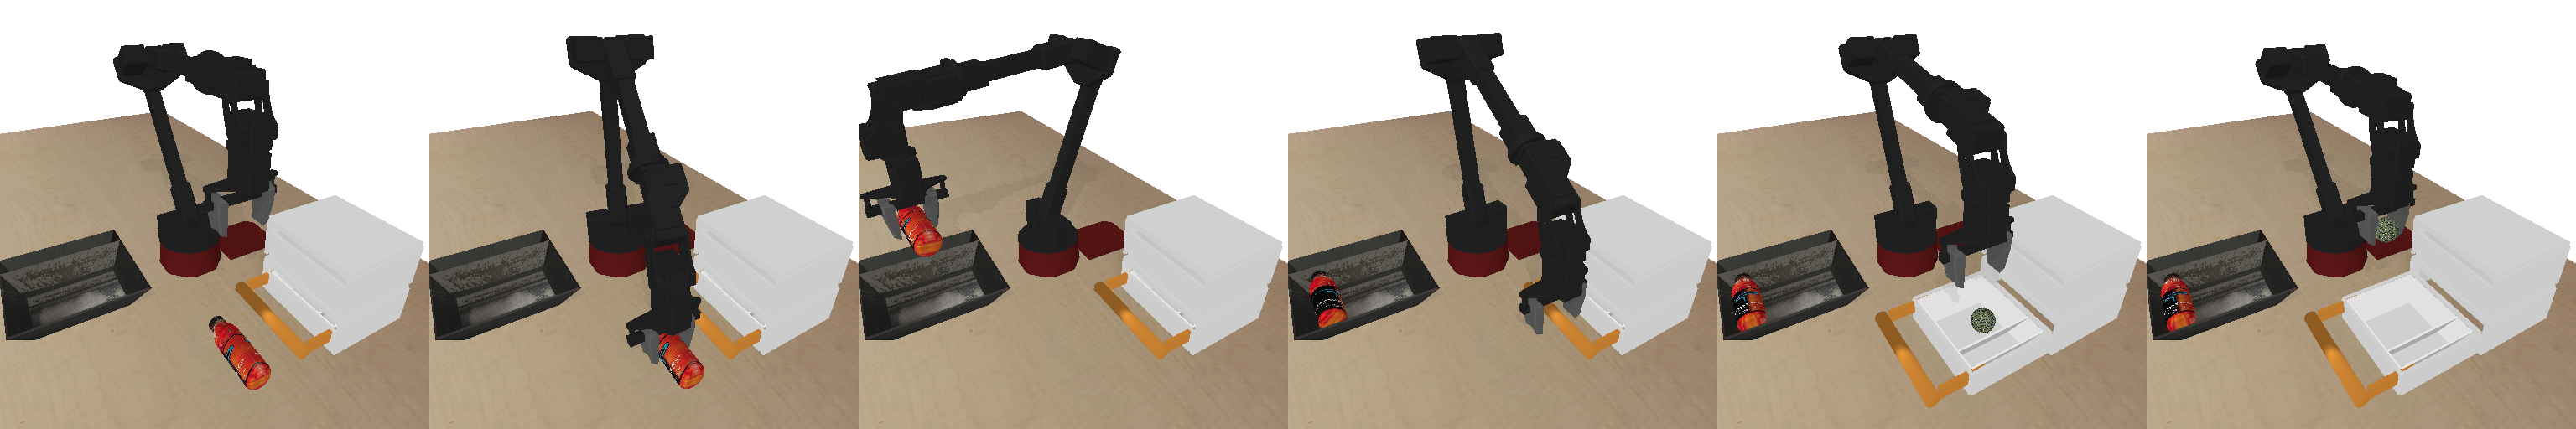
\includegraphics[width=\linewidth]{chapters/dr3/figures/pickplace_open_grasp.png}
    \vspace{-0.1in}
    \caption{\footnotesize{{\textbf{Trend of effective rank,} $\mathrm{srank}(\Phi)$ of features $\Phi$ learned by the Q-function when trained with TD error (red, ``Without DR3'') and with TD error + \drmethodname\ (blue, ``With DR3'') on three Atari games using the 5\% dataset. Note that \drmethodname\ alleviates rank collapse, without explicitly aiming to.}}}
    \label{fig:iup_is_fixed}
    % \vspace{-0.1in}
\end{figure}

\textbf{{{DR3 does not suffer from rank collapse.}}} Prior work~\citep{kumar2021implicit} has shown that implicit regularization can lead to a rank collapse issue in TD-learning, preventing Q-networks from using full capacity. To see if \drmethodname\ addresses the rank collapse issue, we follow \citet{kumar2021implicit} and plot the effective rank of learned features with DR3 in Figure~\ref{fig:iup_is_fixed} {(DQN, REM in Appendix~\ref{app:rank_collapse_is_gone})}. 
%%AK: removed definition in the interest of space
% Effective rank of a matrix $\bM \in  \mathbb{R}^{n \times d}, n > d$ for a given threshold $\delta$ is given by: $\mathrm{srank}_\delta(\bM) = \min \{k: \frac{\sum_{i=1}^k \sigma_i(\bM)}{\sum_{i=1}^d \sigma_i(\bM)} \geq 1 - \delta \}$, where $\{\sigma_i(\bM)\}$ denotes the singular values of $\bM$ arranged in decreasing order. 
While the value of the effective rank decreases during training with na\"ive bootstrapping, {we find that rank of DR3 features typically does not collapse}, despite no explicit term encouraging this. 
% as shown in Figure~\ref{fig:iup_is_fixed}.  
Finally, we test the robustness/sensitivity of each layer in the learned Q-network to re-initialization~\citep{zhang2019all} during training and find that DR3 alters the features to behave similarly to supervised learning~(\Figref{fig:robustness}).

%%AK: This discussion is a bit redundant with what is there in the technical section already, so I can just move it there.
\begin{figure}[t]
\small \begin{center}
\vspace{-0.2cm}
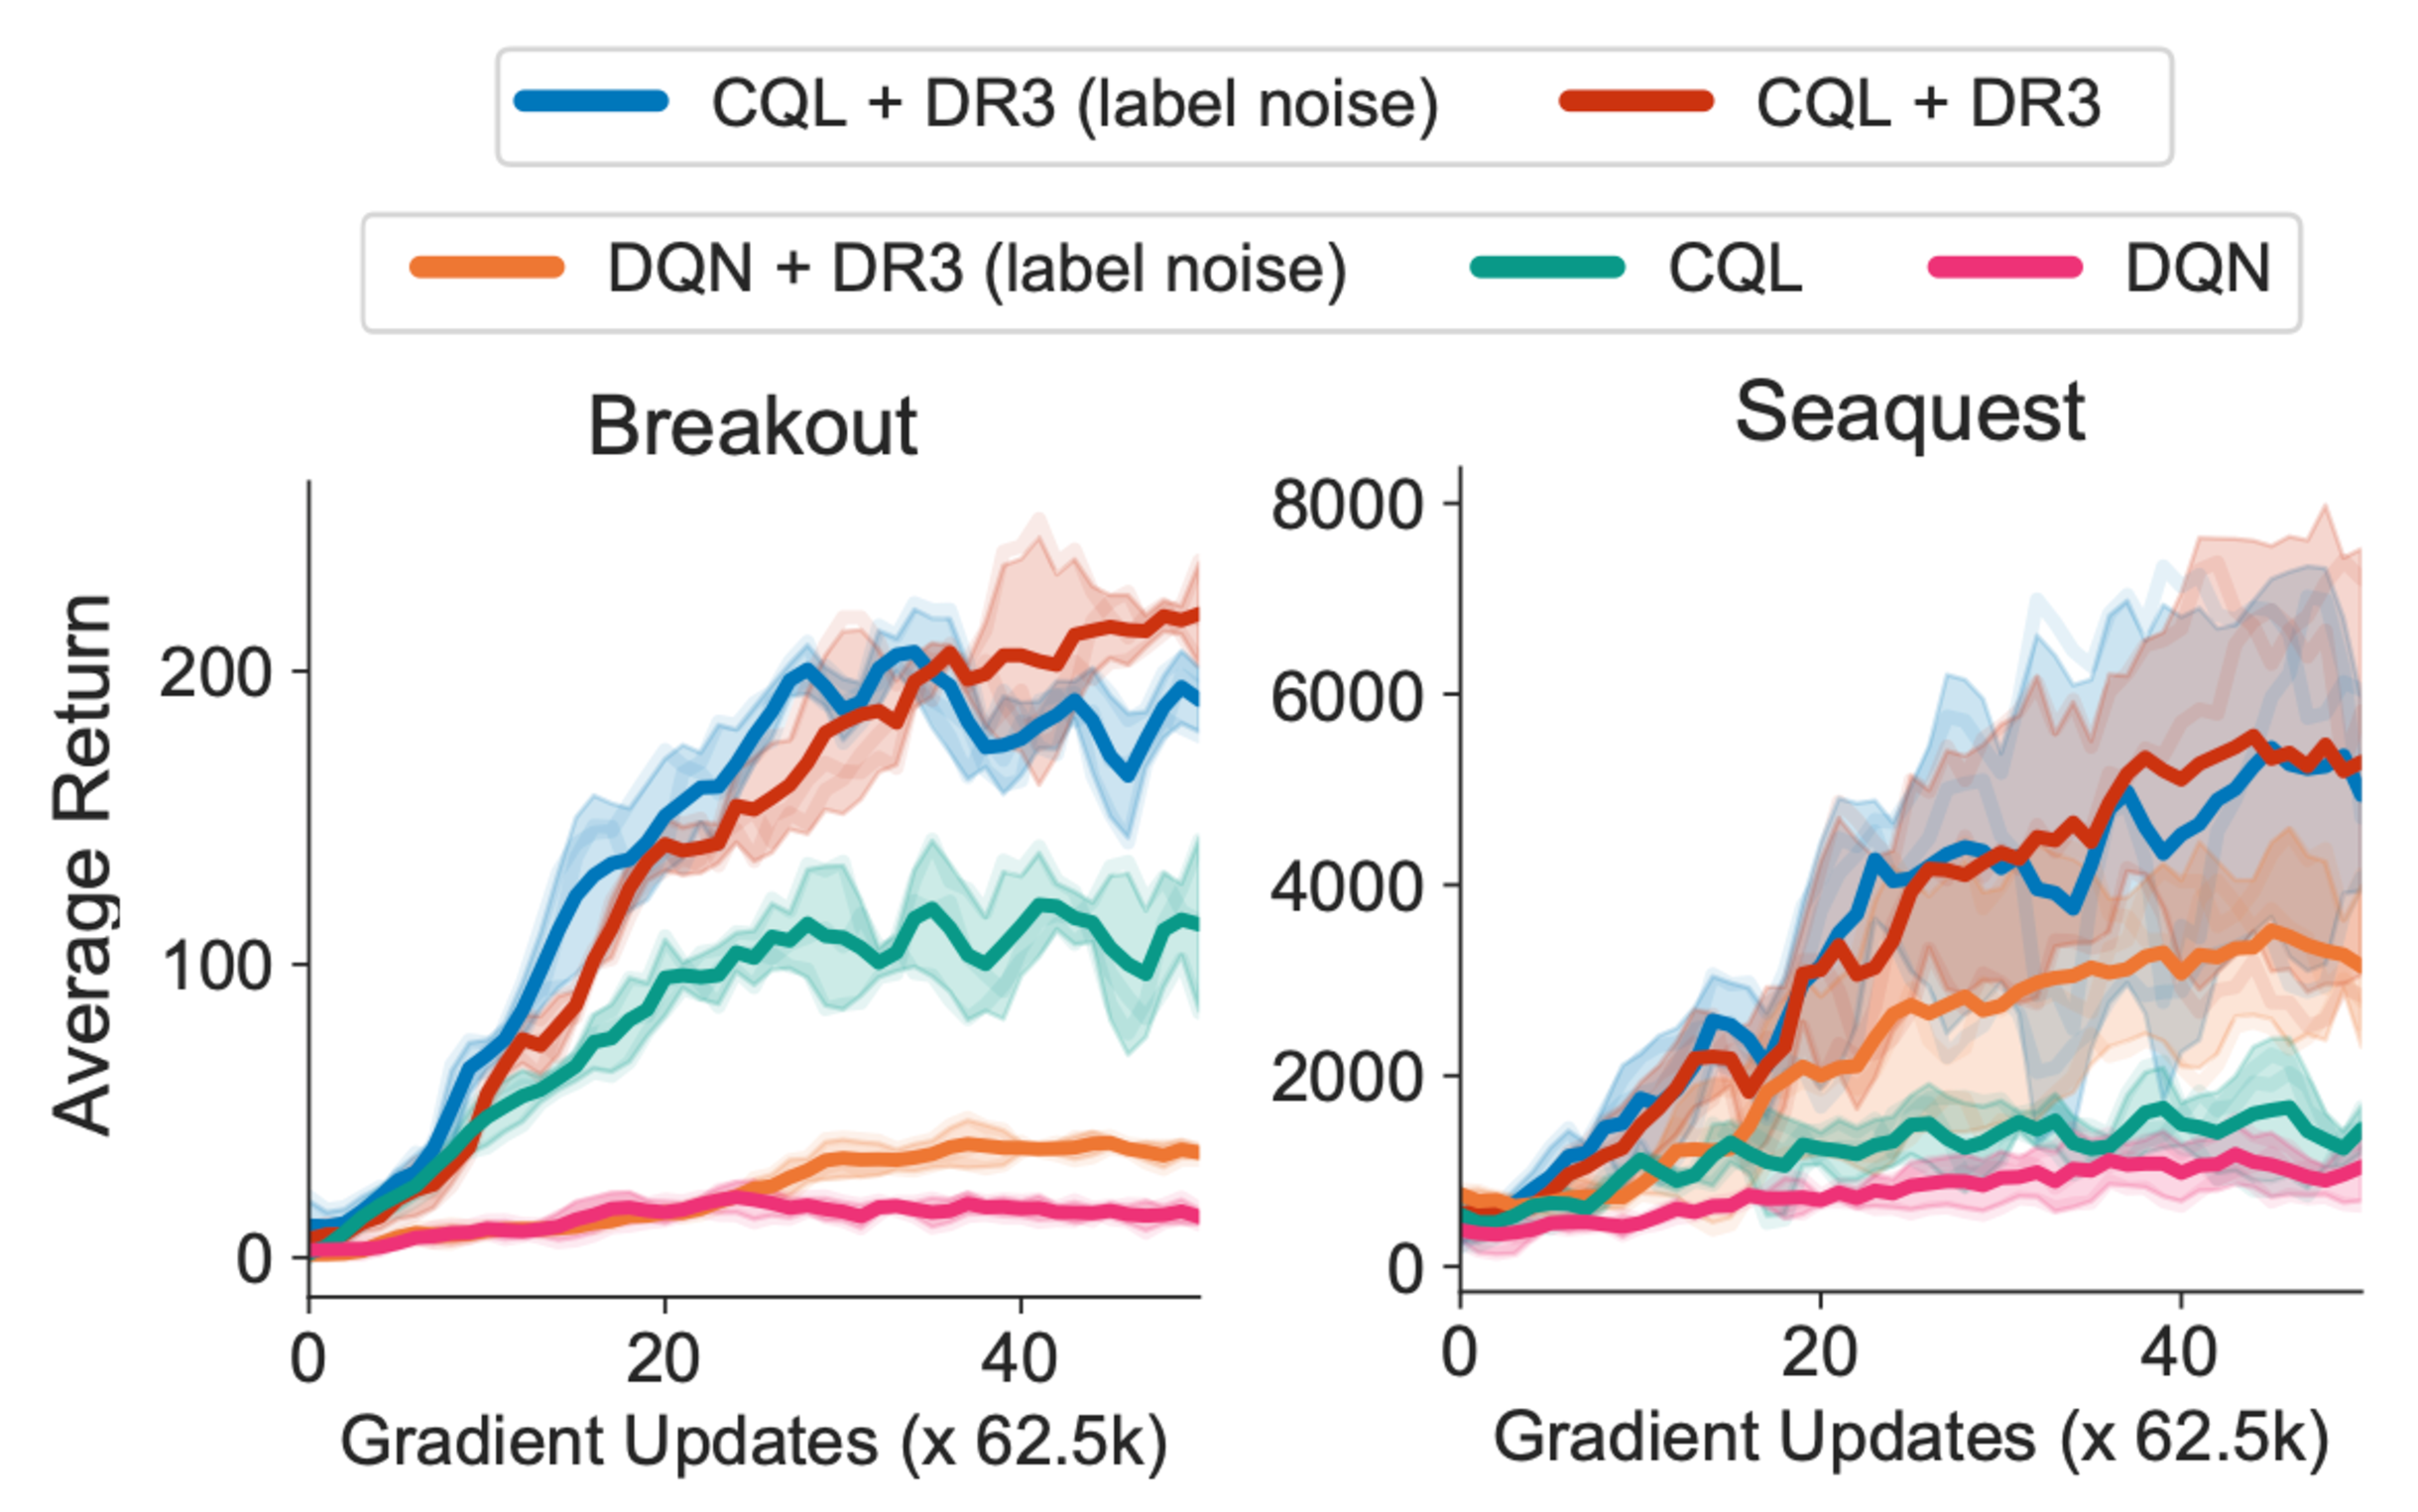
\includegraphics[width=0.6\linewidth]{chapters/dr3/figures_iclr/different_penalty.pdf}
\vspace{-10pt}
\caption{\label{fig:other_penalty_main} \footnotesize{Comparing  DR3 for our simplifying choice of $M$, and $M$ induced by label noise, {with base CQL and DQN algorithms}. Note that both of these penalties when applied over CQL improve performance.}}
\end{center}
% \vspace{-0.2in}
\end{figure}

\textbf{Comparing explicit regularizers for different choices of noise covariance $M$.} Finally, we investigate the behavior of different implicit regularizers derived via two choices of $M$ in Equation~\ref{eqn:regularizer} and the corresponding explicit regularizers. While the explicit regularizer we use in practice is a simplifying choice that works well, another choice of $M$ is the covariance matrix induced by label noise, which requires explicit computation of $\Sigma_M^*$.
%%SL.10.2: This is very important. But I also don't like the weasel words here. We are trying to say that \Sigma_M = I is just another "choice". But critical readers will see right through this. It's not another choice, it's a hack to make it easy to implement, and we should just admit this. It's OK to present an interpretation of it as just another choice for M too, but we should definitely not attempt to hide that it's a hack. Just admit it's a hack, and say we use it because it works well, otherwise reviewers will believe the paper is being deceptive.
Observe in Figure~\ref{fig:other_penalty_main} that the {explicit regularizer for our simplifying choice is not worse than the different choice of $M$}. This justifies utilizing our simplified, heuristic choice of setting $\Sigma_M^* = I$ in practice. Results on five Atari games are shown in Appendix~\ref{app:theory_practice_gap}.       
% Since \drmethodname\ is directly derived as a way to mitigate the undesirable effect of implicit regularization of the TD update, utilizing it directly address the rank collapse issue as compared to a penalty artificially created to tackle ths phenomenon.
% \textbf{Data-Efficient online RL.} Finally, we evaluate the performance of \drmethodname\ on ``data-efficient'' online RL tasks from the Atari-100K benchmark~\citep{kaiser2019model,van2019use}, where the goal is learn a peformant policy as quickly as possible. On these tasks, we apply \drmethodname\ on data-efficient rainbow (DER)~\citep{van2018deep}, and compare the final performance at 100k environment steps.
%%AK: we need to also measure equivalent of average?


% \begin{table}[h]
% \fontsize{8}{8}
% \centering
% \caption{Performance of \drmethodname\ when applied in conjunction with BRAC~\citep{wu2019behavior}. Note that DR3 attains a larger final performance (at the end of 2M steps of training) as well as a higher average performance (i.e. stability score) across all iterations of training.}
% \label{tab:brac}
% \vspace{0.2cm}
% \begin{tabular}{ccccc}
% \toprule
% \multirow{2}{*}{Task} & \multicolumn{2}{c}{Average Performance}   & \multicolumn{2}{c}{Final Performance} \\
% & BRAC & BRAC + \drmethodname & BRAC & BRAC + \drmethodname \\
% \midrule
% %('True', '0.1', '2')
% halfcheetah-exp & 1.7 $\pm$ 1.9 & 49.9 $\pm$ 16.7  & 2.1 $\pm$ 3.3 & 71.5 $\pm$ 24.9 \\
% halfcheetah-med & 43.5 $\pm$ 0.2 & 43.2 $\pm$ 0.2  & 45.1 $\pm$ 0.8 & 44.9 $\pm$ 0.6 \\
% halfcheetah-med-exp & 17.0 $\pm$ 5.4 & 6.0 $\pm$ 5.5  & 24.8 $\pm$ 9.3 & 6.7 $\pm$ 7.3 \\
% halfcheetah-rand & 24.4 $\pm$ 0.4 & 18.4 $\pm$ 0.3  & 24.9 $\pm$ 0.8 & 18.2 $\pm$ 1.0 \\
% % halfcheetah-med-replay & 44.9 $\pm$ 0.3 & 44.1 $\pm$ 0.4  & 45.0 $\pm$ 1.4 & 44.9 $\pm$ 0.5 \\
% hopper-exp & 15.7 $\pm$ 1.5 & 21.8 $\pm$ 3.2  & 16.6 $\pm$ 6.0 & 20.8 $\pm$ 5.3 \\
% hopper-med & 32.8 $\pm$ 1.4 & 46.3 $\pm$ 7.1  & 36.2 $\pm$ 1.7 & 58.3 $\pm$ 13.7 \\
% hopper-med-exp & 40.2 $\pm$ 5.7 & 37.0 $\pm$ 2.9  & 31.7 $\pm$ 11.8 & 21.8 $\pm$ 4.9 \\
% hopper-rand-v0 & 11.7 $\pm$ 0.0 & 11.2 $\pm$ 0.0  & 12.2 $\pm$ 0.0 & 11.1 $\pm$ 0.0 \\
% hopper-med-replay & 31.6 $\pm$ 0.3 & 30.3 $\pm$ 0.8  & 31.3 $\pm$ 1.2 & 36.1 $\pm$ 5.7 \\
% walker2d-exp & 25.5 $\pm$ 14.4 & 33.6 $\pm$ 11.8  & 54.0 $\pm$ 31.0 & 60.6 $\pm$ 20.2 \\
% walker2d-med & 81.3 $\pm$ 0.3 & 80.8 $\pm$ 0.2  & 83.8 $\pm$ 0.2 & 83.4 $\pm$ 0.3 \\
% walker2d-med-exp & 5.8 $\pm$ 5.2 & 6.4 $\pm$ 3.4  & 22.4 $\pm$ 22.0 & 39.5 $\pm$ 23.3 \\
% walker2d-rand & 1.4 $\pm$ 0.8 & 1.7 $\pm$ 0.9  & 0.0 $\pm$ 0.1 & 2.9 $\pm$ 2.1 \\
% walker2d-med-replay & 26.1 $\pm$ 6.4 & 47.4 $\pm$ 4.1  & 11.7 $\pm$ 7.0 & 38.7 $\pm$ 9.6 \\
% \midrule
% Median Normalized Perf. & 25.5 & \textbf{33.6} & 24.9 & \textbf{38.7} \\
% Mean Normalized Perf. & 26.9 & \textbf{31.9} & 29.5 & \textbf{37.3} \\
% \bottomrule
% \end{tabular}
% \end{table}









% \subsection{Offline Policy Evaluation}
% d4rl, cite DOPE benchmark, FQE is best already
% comparable on most tasks, and improvements on a few tasks. Antmaze and mujoco similar.
% \begin{figure*}[t]
%     \centering
%     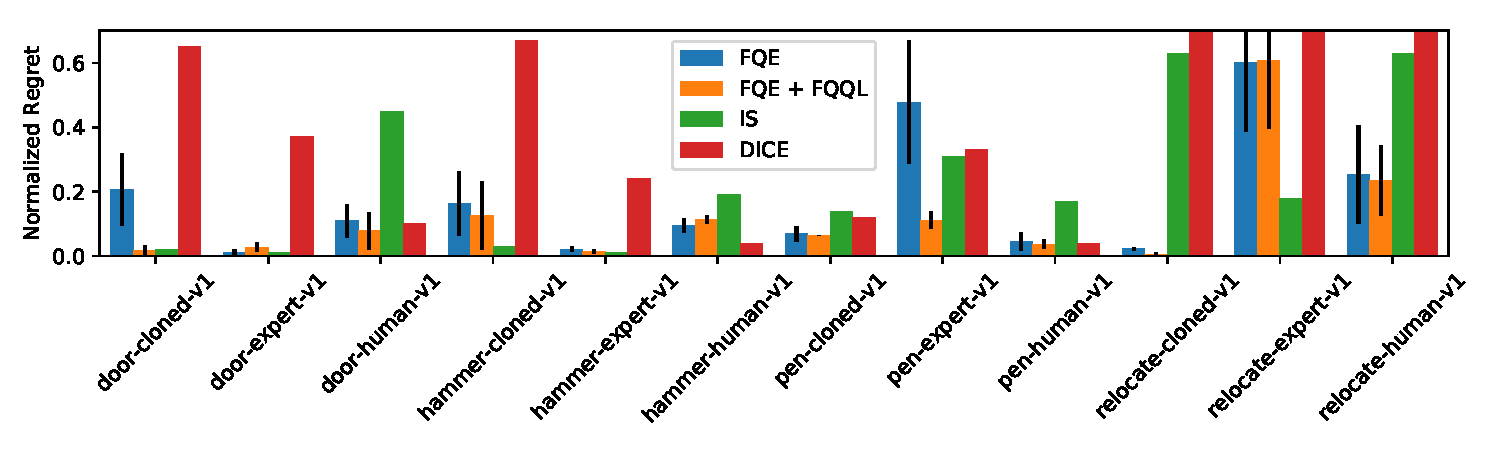
\includegraphics[width=\linewidth]{chapters/dr3/figures/Normalized Regret.pdf}
%     \vspace{-0.65cm}
%     \caption{Normalized regret on harder benchmark offline policy evaluations tasks in the DOPE benchmark~\citep{fu2021benchmarks}. Lower regret is better. We report the mean over 5 seeds and SEM. We use the benchmark numbers for IS and DICE from~\citep{fu2021benchmarks}.}
%     \label{fig:fqe}
% \end{figure*}

% \vspace{-8pt}
% \section{Experimental Evaluation of \drmethodname}
% \label{sec:experiments}
% \vspace{-8pt}
% % The goal of our experiments is to verify the claim that value-based deep RL methods require explicit regularization, as well as to evaluate the efficacy of our practical approach, \drmethodname, in addressing regularization challenges.
% %%SL.10.2: I wonder if some readers might question whether our experiments really verify that it *requires* explicit regularization. We could say rather it aims to understand whether feature co-adaptation is a major issue empirically or something. But it actually doesn't look like the experiments do that at all, and only focus on DR3? In that case, we could simply say: Our experiments aim to evaluate the extent to which \drmethodname improves performance in offline RL in practice, as well as to study its effect on rank collapse and how it compares to the more costly but more accurate regularizer suggested by our theoretical analysis, which requires estimating $\Sigma_M^\star$. (or something along these lines)
% Our experiments aim to evaluate the extent to which \drmethodname\ improves performance in offline RL in practice, and to study its effect on prior observations of rank collapse and how it compares to the more costly regularizer suggested by our analysis, which requires estimating $\Sigma_M^\star$. To this end, we investigate if \drmethodname\ improves offline RL performance and stability on three offline RL benchmarks: Atari 2600 games with discrete actions~\citep{agarwal2019optimistic}, continuous control tasks from D4RL~\citep{fu2020d4rl}, and image-based robotic manipulation tasks~\citep{singh2020cog}.
% % Additionally, we present experiments to understand the effects of \drmethodname\ on the features learned by the Q-network and verify if it does indeed make TD learning behave like supervised learning.
% %%SL.9.29: can probably cut this last sentence


% % \textbf{Evaluation metrics.} Prior works in offline RL report either the final performance after an arbitrary fixed number of iterations~ or the best performance (as measured via online rollouts) over those iterations~\citep{gulcehre2020rl, agarwal2019optimistic}. Both protocols are problematic, since the former requires selecting the iteration count carefully, while the latter requires a large number of online rollouts, defeating the point of offline RL.
% % Therefore, 
% Following prior work~\citep{fu2020d4rl, gulcehre2020rl}, we evaluate DR3 in terms of final offline RL performance after a given number of iterations. Additionally, we report \emph{training stability}, which is important in practice as offline RL does not admit cheap validation of trained policies for model selection.
% % Prior work has generally disregarded this metric, reporting results either after a hand-selected number of gradient steps~\citep[\textit{e.g.,}][]{wu2019behavior,fu2020d4rl,kumar2020conservative}, or the maximum performance  during training (i.e., oracle model selection)~\citep{agarwal2019optimistic, gulcehre2020rl}.
% %%SL.9.29: if short on space, can cut the sentences below and merge the next paragraph with this one
% % We argue that neither final nor best achieved performance gives a complete picture of performance, since in practice selecting the number of training gradient steps precisely is both important for strong performance and difficult to do without online evaluation.
% % %%AK: The situation hopefully has a bit changed now :). We have some ways of doing checkpoint selection, which will hopefully be improved soon. Not sure if we want to cite the workflow paper? But then this becomes too circular (that paper cites this paper)...
% % This can make unstable algorithms appear to perform much better on benchmarks than they would in real-world settings.
% To evaluate stability, we train for a large number of gradient steps (2-3x longer than prior work) and either report the \textbf{average performance} over the course of training or the final performance at the end of training. %In expectation, this metric is equivalent to the average expected final performance obtained if we randomly picked a iteration to evaluate. 
% %%AK; commenting the line below since practitioners always have domain info, also cuts space and not sure it is adding much anways
% % Such a uniform-at-random policy selection scheme is what practitioners are likely to use in practice if no domain information is available. 
% % In other words, this metric assumes a uniform-at-random policy selection scheme, which resembles one practitioners are likely to use in practice if no domain information is available. 
% We expect that a stable method that does not unlearn with more gradient steps, should have better average performance, as compared to a method that attains good peak performance but degrades with more training. See Appendix~\ref{app:additional_background} for further details.
% % and not the number of environment steps (since the setting is completely offline).
% %%SL.5.23: maybe mention that you also show learning curves? it would help to explain these learning curves, because they don't show what readers necessarily expect in RL (where x-axis = amount of data), but rather number of grad steps.
% % \todo{Link to appendix}

% % \begin{figure*}[h]
% %     \centering
% %     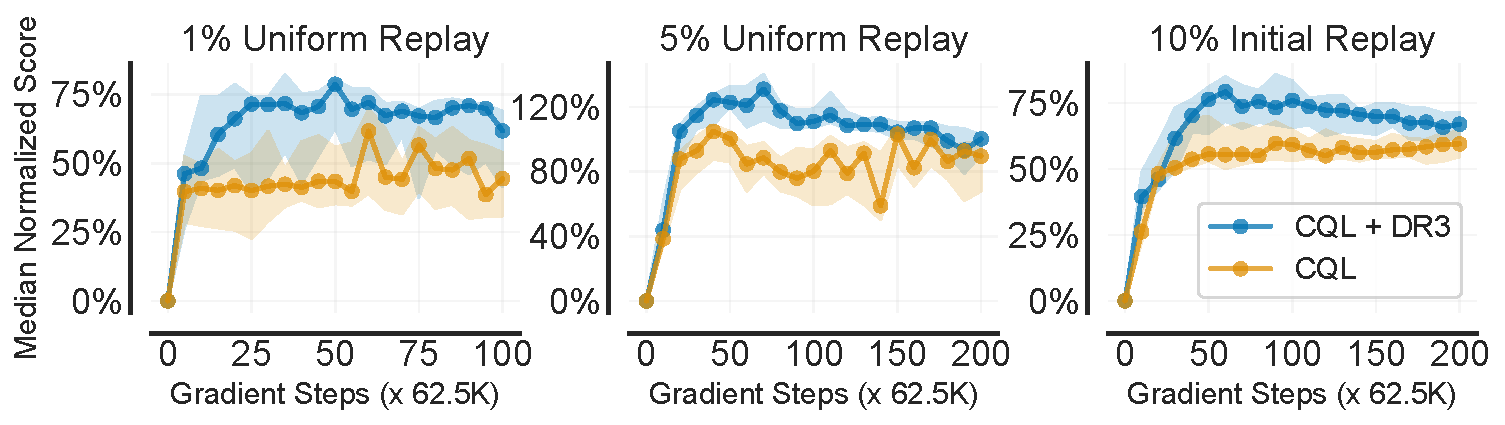
\includegraphics[width=\linewidth]{chapters/dr3/figures/atari_new/Median_cql_penalty.pdf}
% %     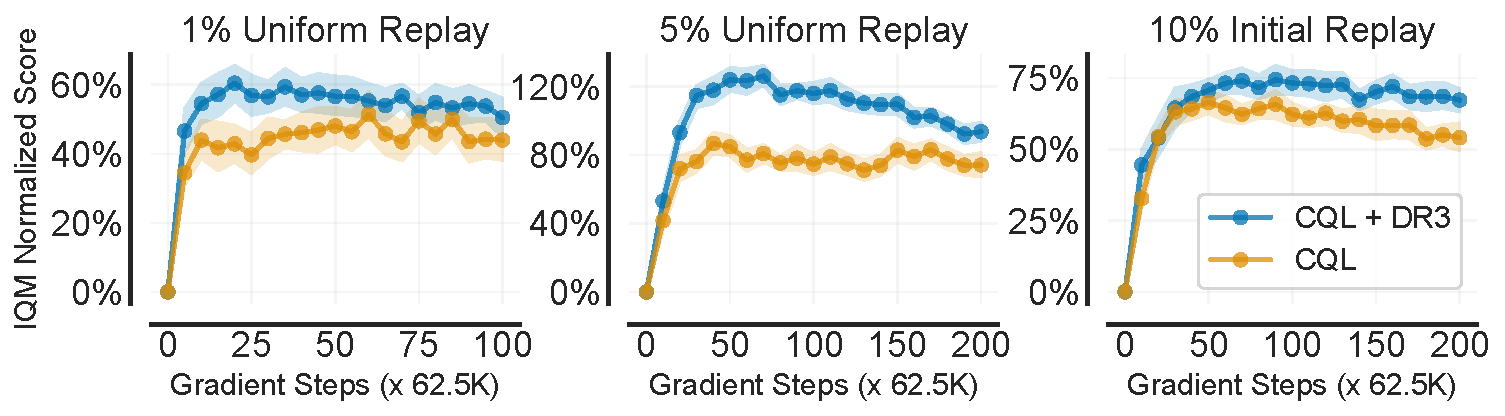
\includegraphics[width=\linewidth]{chapters/dr3/figures/atari_new/IQM_cql_penalty.pdf}
% %     % 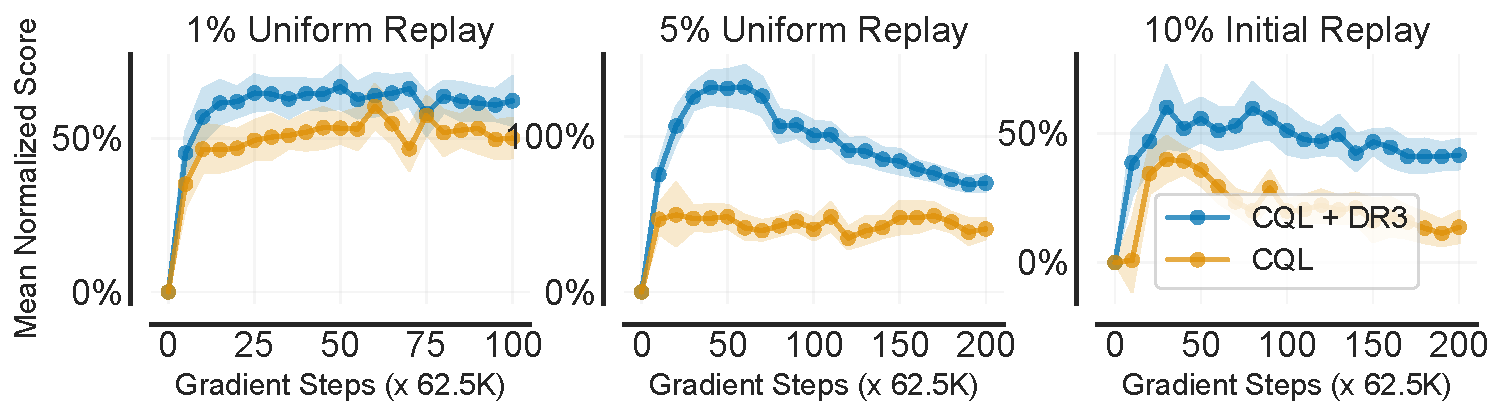
\includegraphics[width=\linewidth]{chapters/dr3/figures/atari_new/Mean_cql_penalty.pdf}
% %     % 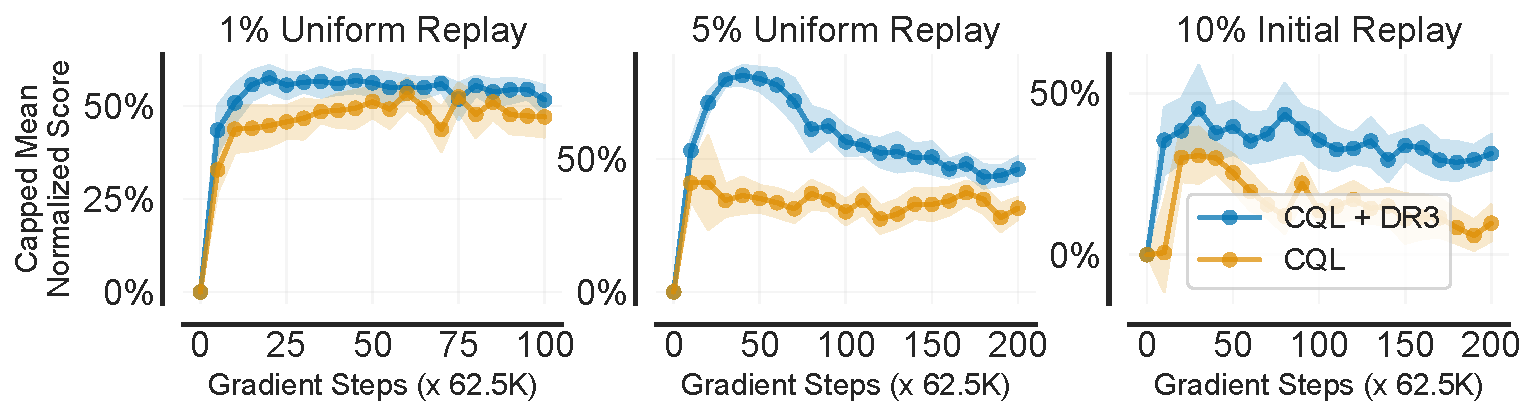
\includegraphics[width=\linewidth]{chapters/dr3/figures/atari_new/Capped_Mean_cql_penalty.pdf}
% %     \vspace{-0.65cm}
% %     \caption{Behavior Normalized Scores across 17 Atari games. We use Interquartile mean~(IQM).}
% %     \label{fig:atari_5_percent}
% % \end{figure*}



% % \begin{figure}[t]
% %     \centering
% %     \includegraphics[width=\linewidth]{atari/norm_3_games_cql_rem.pdf}
% %     \vspace{-0.65cm}
% %     \caption{In addition to minimizing unnormalized similarities~($\simunnorm(\bs, \ba, \bs')$), \drmethodname\ attains much lower normalized similarities as compared to CQL and REM. The results are shown for training with 5\% DQN replay dataset averaged over 5 seeds.}\label{fig:atari_3_cosine}
% %     \vspace{-0.5cm}
% % \end{figure}


% % \begin{figure*}[t]
% %     \centering
% %     \includegraphics[width=\linewidth]{atari/5_percent_res_100.pdf}
% %     \vspace{-0.65cm}
% %     \caption{Evaluation performance of offline REM and CQL with and without \drmethodname\ on the 5\% DQN replay dataset~\citep{agarwal2019optimistic}. Note that the data collected during evaluation is not provided to offline agents during training. The horizontal line shows the average performance of the trajectories in entire DQN replay dataset. \drmethodname\ substantially improves the performance of CQL and REM as well as prevents the decay in performance of REM with more gradient updates on \textsc{Seaquest} and \textsc{Asterix}. For \textsc{Pong}, training for longer~(12.5 million updates) results in improved score for REM + \drmethodname\ over REM.}
% %     \label{fig:atari_5_percent}
% % \end{figure*}


% % \begin{table*}[t]
% %     \centering
% %     \caption{Normalized returns on sub-sampled Atari DQN Replay datasets~\citep{agarwal2019optimistic}. A random policy is provided a normalized score of zero while the average performance of the trajectories in the entire DQN replay dataset is assigned a normalized score of 100. We report results based on 6.5 million gradient updates with batch size of 32 for the 1\% setting and 12.5 million gradient updates for the 5\% and 10\% settings. The individual scores and learning curves for all the 17 games are provided in the Appendix~\ref{app:atari_results}.}
% %     \label{tab:cql_res}
% %     \vspace{0.2cm}
% % \begin{tabular}{cccccc}
% % \toprule
% % %%AK.1.26: maybe we want to name the average performance as Stability coefficient or something like that but thats a minor point
% % \multirow{2}{*}{DQN Replay Setting} & Normalized Score Metric & \multicolumn{2}{c}{Average Performance}   & \multicolumn{2}{c}{Maximum Performance} \\
% % & (17 games) & CQL & CQL + \drmethodname & CQL & CQL + \drmethodname \\
% % \midrule
% % 1\% replay &  Median & 43.3 & \textbf{71.0} & 73.2 & \textbf{96.3} \\
% % (uniformly sampled) & Mean & 50.7 & \textbf{60.9} & 74.4 & \textbf{84.6}  \\
% % \midrule
% % {5\% replay} & Median  & 84.6 & \textbf{104.9} & 127.8 & \textbf{150.7} \\
% % (uniformly sampled)  & Mean & 43.3 & \textbf{97.2} &  139.5 & \textbf{189.5}  \\
% % \midrule
% % {10\% replay} & Median  & 53.4 &  \textbf{69.9} & 73.3 & \textbf{97.2} \\
% % (initial exploration data) & Mean & 21.8 & \textbf{49.6} &  79.4 & \textbf{140.0}  \\
% % \bottomrule
% % \end{tabular}
% % \end{table*}

% %% Final Performance CQL vs Penalty
% % -----DR3+CQL-----
% % *****Median*****
% % 1% data
% % Median 61.8 [41.6 69. ]
% % 5% data
% % Median 100.2 [ 90.6 102.7]
% % 10% data
% % Median 67.0 [62.1 71.4]
% % *****IQM*****
% % 1% data
% % IQM 50.5 [44.9 56.1]
% % 5% data
% % IQM 93.6 [88. 99.]
% % 10% data
% % IQM 67.3 [63.2 71.4]
% % -----CQL-----
% % *****Median*****
% % 1% data
% % Median 44.4 [30.9 54. ]
% % 5% data
% % Median 89.6 [67.9 98.2]
% % 10% data
% % Median 59.6 [54.6 64.4]
% % *****IQM*****
% % 1% data
% % IQM 44.0 [38.1 49.8]
% % 5% data
% % IQM 74.2 [67.3 81.4]
% % 10% data
% % IQM 54.1 [49.5 59.3]

% %% Final performance REM vs REM+penalty
% % -----DR3+REM-----
% % *****Median*****
% % 1% data
% % Median 13.1 [10.  18.4]
% % 5% data
% % Median 72.4 [65.7 81.1]
% % 10% data
% % Median 72.4 [65.7 81.1]
% % *****IQM*****
% % 1% data
% % IQM 13.4 [11.  16.4]
% % 5% data
% % IQM 77.2 [71.4 83.9]
% % 10% data
% % IQM 77.2 [71.4 83.9]
% % -----REM-----
% % *****Median*****
% % 1% data
% % Median -0.0 [-0.7  0.1]
% % 5% data
% % Median 24.9 [14.5 29. ]
% % 10% data
% % Median 24.9 [14.5 29. ]
% % *****IQM*****
% % 1% data
% % IQM -0.1 [-0.7  0.6]
% % 5% data
% % IQM 23.5 [19.9 27.3]
% % 10% data
% % IQM 23.5 [19.9 27.3]


% % REM vs REM + penalty Average performance (stability)
% % -----DR3+REM-----
% % *****Median*****
% % 1% data
% % Median 11.7
% % 5% data
% % Median 52.5
% % 10% data
% % Median 63.9
% % *****IQM*****
% % 1% data
% % IQM 12.4
% % 5% data
% % IQM 53.5
% % 10% data
% % IQM 67.8
% % -----REM-----
% % *****Median*****
% % 1% data
% % Median 3.1
% % 5% data
% % Median 18.8
% % 10% data
% % Median 47.7
% % *****IQM*****
% % 1% data
% % IQM 3.4
% % 5% data
% % IQM 21.1
% % 10% data
% % IQM 47.9

% % FInal performance (scaled via random scores and CQL is 100\% for IUP comparison):
% % Asterix 256.6
% % BeamRider 18.6
% % Breakout 176.3
% % DemonAttack 228.0
% % DoubleDunk 133.5
% % Enduro 115.2
% % IceHockey 51.7
% % Jamesbond 310.8
% % MsPacman 131.5
% % Pong 105.5
% % Qbert 114.4
% % RoadRunner 100.0
% % Seaquest 366.6
% % SpaceInvaders 322.8
% % WizardOfWor 80.3
% % YarsRevenge 75.7
% % Zaxxon 485.6



% % \begin{table*}[t]
% %     \centering
% %     \caption{Normalized returns on sub-sampled Atari DQN replay datasets~\citep{agarwal2019optimistic}. The individual scores and learning curves for all the 17 games are provided in the Appendix~\ref{app:atari_results}. When combined with REM, we used a coefficient of $\alpha = 0.001$ to show the robustness of \drmethodname\ across different datasets. \color{red}{Merge the two tables somehow to save space.}}
% %     \label{tab:rem_res}
% %     \vspace{0.2cm}
% % \begin{tabular}{cccccc}
% % \toprule
% % %%AK.1.26: maybe we want to name the average performance as Stability coefficient or something like that but thats a minor point
% % \multirow{2}{*}{DQN Replay Setting} & Normalized Score Metric & \multicolumn{2}{c}{Average Performance}   & \multicolumn{2}{c}{Maximum Performance} \\
% % & (17 games) & REM & REM + \drmethodname & REM & REM + \drmethodname \\
% % \midrule
% % 1\% replay &  Median & 4.7 & \textbf{19.3} & 25.5 & \textbf{42.5} \\
% % (uniformly sampled) & Mean & -1.8 & \textbf{47.2} &  72.4 & \textbf{100.2}  \\
% % \midrule
% % {5\% replay} & Median  & 27.4 & \textbf{58.5} & 88.8 & \textbf{99.8} \\
% % (uniformly sampled)  & Mean & 40.9 & \textbf{84.7} &  141.1 & \textbf{165.8}  \\
% % \midrule
% % {10\% replay} & Median  & 50.7 &  \textbf{68.5} & 107 & \textbf{108.5} \\
% % (initial exploration data) & Mean & 63.7 & \textbf{84.4} &  136.5 & \textbf{140.7}  \\
% % \bottomrule
% % \end{tabular}
% % \end{table*}

% %% Final Performance CQL vs Penalty
% % -----DR3+CQL-----
% % *****Median*****
% % 1% data
% % Median 61.8 [41.6 69. ]
% % 5% data
% % Median 100.2 [ 90.6 102.7]
% % 10% data
% % Median 67.0 [62.1 71.4]
% % *****IQM*****
% % 1% data
% % IQM 50.5 [44.9 56.1]
% % 5% data
% % IQM 93.6 [88. 99.]
% % 10% data
% % IQM 67.3 [63.2 71.4]
% % -----CQL-----
% % *****Median*****
% % 1% data
% % Median 44.4 [30.9 54. ]
% % 5% data
% % Median 89.6 [67.9 98.2]
% % 10% data
% % Median 59.6 [54.6 64.4]
% % *****IQM*****
% % 1% data
% % IQM 44.0 [38.1 49.8]
% % 5% data
% % IQM 74.2 [67.3 81.4]
% % 10% data
% % IQM 54.1 [49.5 59.3]

% % CQL  vs CQL + penalty Average performance (stability)
% % -----DR3+CQL-----
% % *****Median*****
% % 1% data
% % Median 63.7
% % 5% data
% % Median 102.6
% % 10% data
% % Median 65.2
% % *****IQM*****
% % 1% data
% % IQM 52.6
% % 5% data
% % IQM 102.4
% % 10% data
% % IQM 65.2
% % -----CQL-----
% % *****Median*****
% % 1% data
% % Median 42.5
% % 5% data
% % Median 81.4
% % 10% data
% % Median 52.1
% % *****IQM*****
% % 1% data
% % IQM 42.8
% % 5% data
% % IQM 72.3
% % 10% data
% % IQM 56.3


% % \begin{table*}[t]
% %     \centering
% %     \caption{\small{Performance of REM, REM + \drmethodname after 6.5M gradient steps for the 1\% setting and 12.5M gradient steps for the 5\%, 10\% settings. Individual scores for all 17 games are provided in the Appendix~\ref{app:atari_results}.}}
% %     \label{tab:rem_res}
% %     \vspace{0.2cm}
% % \begin{tabular}{cccccc}
% % \toprule
% % \multirow{2}{*}{\textbf{Data}} & \textbf{Metric} & \multicolumn{2}{c}{\textbf{Last iteration score}}   & \multicolumn{2}{c}{\textbf{Stability score}} \\
% % & (17 games) & REM & REM + \drmethodname & REM & REM + \drmethodname \\
% % \midrule
% % 1\% &  Median & 0.0 & \textbf{13.1} & 3.1 & \textbf{11.7} \\
% %  & IQM & -0.1 & \textbf{13.4} & 3.4 & \textbf{12.4}  \\
% % \midrule
% % 5\% & Median  & 24.9 & \textbf{72.4} & 18.8 & \textbf{52.5} \\
% %  & IQM & 23.5 & \textbf{77.2} &  21.1 & \textbf{53.5}  \\
% % \midrule
% % 10\% & Median & 24.9 &  \textbf{72.4} & 47.7 & \textbf{63.9} \\
% %  & IQM & 23.5 & \textbf{77.4} &  47.9 & \textbf{67.8}  \\
% % \bottomrule
% % \end{tabular}
% % \end{table*}



% % REM vs REM + penalty Average performance (stability)
% % -----DR3+REM-----
% % *****Median*****
% % 1% data
% % Median 11.7
% % 5% data
% % Median 52.5
% % 10% data
% % Median 63.9
% % *****IQM*****
% % 1% data
% % IQM 12.4
% % 5% data
% % IQM 53.5
% % 10% data
% % IQM 67.8
% % -----REM-----
% % *****Median*****
% % 1% data
% % Median 3.1
% % 5% data
% % Median 18.8
% % 10% data
% % Median 47.7
% % *****IQM*****
% % 1% data
% % IQM 3.4
% % 5% data
% % IQM 21.1
% % 10% data
% % IQM 47.9

% %% Final performance REM vs REM+penalty
% % -----DR3+REM-----
% % *****Median*****
% % 1% data
% % Median 13.1 [10.  18.4]
% % 5% data
% % Median 72.4 [65.7 81.1]
% % 10% data
% % Median 72.4 [65.7 81.1]
% % *****IQM*****
% % 1% data
% % IQM 13.4 [11.  16.4]
% % 5% data
% % IQM 77.2 [71.4 83.9]
% % 10% data
% % IQM 77.2 [71.4 83.9]
% % -----REM-----
% % *****Median*****
% % 1% data
% % Median -0.0 [-0.7  0.1]
% % 5% data
% % Median 24.9 [14.5 29. ]
% % 10% data
% % Median 24.9 [14.5 29. ]
% % *****IQM*****
% % 1% data
% % IQM -0.1 [-0.7  0.6]
% % 5% data
% % IQM 23.5 [19.9 27.3]
% % 10% data
% % IQM 23.5 [19.9 27.3]

% % \begin{table*}[t]
% %     \centering
% %     \caption{\small{Performance of REM, REM + \drmethodname after 6.5M gradient steps for the 1\% setting and 12.5M gradient steps for the 5\%, 10\% settings. Individual scores for all 17 games are provided in the Appendix~\ref{app:atari_results}.}}
% %     \label{tab:rem_res}
% %     \vspace{0.2cm}
% % \begin{tabular}{cccccc}
% % \toprule
% % \multirow{2}{*}{\textbf{Data}} & \textbf{Metric} & \multicolumn{2}{c}{\textbf{Last iteration score}}   & \multicolumn{2}{c}{\textbf{Stability score}} \\
% % & (17 games) & REM & REM + \drmethodname & REM & REM + \drmethodname \\
% % \midrule
% % 1\% &  Median & 0.0 & \textbf{13.1} & 3.1 & \textbf{11.7} \\
% %  & IQM & -0.1 & \textbf{13.4} & 3.4 & \textbf{12.4}  \\
% % \midrule
% % 5\% & Median  & 24.9 & \textbf{72.4} & 18.8 & \textbf{52.5} \\
% %  & IQM & 23.5 & \textbf{77.2} &  21.1 & \textbf{53.5}  \\
% % \midrule
% % 10\% & Median & 24.9 &  \textbf{72.4} & 47.7 & \textbf{63.9} \\
% %  & IQM & 23.5 & \textbf{77.4} &  47.9 & \textbf{67.8}  \\
% % \bottomrule
% % \end{tabular}
% % \end{table*}

% % \begin{wrapfigure}{r}{0.57\textwidth}
% %     \centering
% %     \vspace{-5pt}
% %     \includegraphics[width=0.99\linewidth]{chapters/dr3/figures/atari_new/IQM_rem_penalty.pdf}
% %     \includegraphics[width=0.99\linewidth]{chapters/dr3/figures/atari_new/IQM_cql_penalty.pdf}
% %     \vspace{-0.25in}
% %     \caption{\small{\textbf{Average normalized performance across 17 Atari games for REM + \drmethodname\ (top), CQL + \drmethodname\ (bottom)} over the course of training with different datasets. x-axis represents \emph{gradient steps}; no new data is collected. While na\"ive REM suffers from a degradation in performance with more training, REM + \drmethodname\ not only remains generally stable with more training, but also attains higher final performance. CQL + \drmethodname\ attains higher performance than CQL. As recommended by \citet{agarwal2021precipice}, we report interquartile Mean (IQM) with stratified bootstrap 95\% CIs as shaded regions.}}
% %     \label{fig:atari_all_combined}
% %     \vspace{-0.45cm}
% % \end{wrapfigure}
% \textbf{{Offline RL on Atari 2600 games.}} We compare \drmethodname\ to prior offline RL methods on a set of offline Atari datasets of varying sizes and quality, akin to \citet{agarwal2019optimistic, kumar2021implicit}. We evaluated on three datasets: \textbf{(1)} 1\% and 5\% samples drawn uniformly at random from DQN replay; \textbf{(2)} a dataset with more suboptimal data consisting of the first 10\% samples observed by an online DQN. Following \citet{agarwal2021precipice}, we report the interquartile mean~(IQM) normalized scores across 17 games over the course of training in Figure~\ref{fig:atari_all_combined} and report the IQM average performance in Table~\ref{tab:cql_res}. Observe that combining \drmethodname\ with modern offline RL methods (CQL, REM) attains the best final and average performance across the 17 Atari games tested on, directly improving upon prior methods
% across all the datasets. When \drmethodname\ is used in conjunction with REM, it prevents unlearning and performance degradation with more training. CQL + \drmethodname\ improves by \textbf{20\%} over CQL on final performance and attains \textbf{25\%} better average performance. We also compare \drmethodname\ to the $\mathrm{srank}(\Phi)$ penalty proposed to counter rank collapse~\citep{kumar2021implicit}. Directly taking median normalized score improvements reported by \citet{kumar2021implicit}, CQL + \drmethodname\ improves by over \textbf{2x} (31.5\%) over na\"ive CQL relative to the srank penalty~(14.1\%), indicating DR3's efficacy.
% % this $\text{srank}$ penalty only attains a median improvement of 14.1\% over na\"ive CQL, whereas CQL + \drmethodname\ attains a median improvement of \textbf{31.5\%} over CQL. Thus, CQL + \drmethodname\ improves by over \textbf{2x} relative to the srank penalty, indicating DR3's efficacy.
% % This indicates that by directly addressing the adverse impacts of implicit regularization, \drmethodname\ can substantially improve upon prior methods that only address its symptoms.  

% %Notably, REM performs similar to a random policy in terms of average performance on the 1\%  setting, which is significantly improved by \drmethodname.
% %%SL.2.1: I think we can cut this last sentence, and instead focus on the more positive takeaways.

% % To evaluate whether the improvements from \drmethodname\ stem from penalizing unnormalized similarities $\simunnorm(\bs, \ba, \bs')$, we also compare \drmethodname\ to penalizing (1) $\simnorm(\bs, \ba, \bs')$, or (2) feature norms~($\|\phi(\bs)\|_2$) on the 5\% dataset on 5 games. The full results, shown in Appendix~\ref{}, confirms that both of these penalties perform substantially worse than \drmethodname, aligned with our theoretical analysis about effectiveness of \drmethodname~(Section~\ref{sec:method_analysis}).

% %%SL.2.1: This last phrase is without context. What question is it trying to answer? What is the motivation? Start with a sentence of motivation or a question, then evidence, then answer. Something like: Is [whatever] true? To answer this question, we can [do something]. The full results, shown in [where], indicate [something]. This suggests that [something].
% \begin{wrapfigure}{r}{0.42\textwidth}
% \small \begin{center}
% \vspace{-15pt}
% \includegraphics[width=0.99\linewidth]{chapters/dr3/figures/close_open_grasp (1).png}
% \includegraphics[width=0.99\linewidth]{chapters/dr3/figures/pickplace_open_grasp.png}
% \vspace{-20pt}
% \end{center}
% \end{wrapfigure}
% \textbf{{Offline RL on robotic manipulation from}} \textbf{{images.}} Next, we aim to evaluate the efficacy of \drmethodname\ on two image-based robotic manipulation tasks~\citep{singh2020cog}~(visualized on the right) that require composition of skills (e.g., opening a drawer, closing a drawer, picking an obstructive object, placing an object, etc.) over extended horizons using only a sparse 0-1 reward. 
% As shown in Figure~\ref{fig:cog_figure}, combining \drmethodname\ with COG not only improves over COG, but also learns faster and attains a better average performance.

% \begin{table}[t]
%     \centering
% \fontsize{8}{8}\selectfont
%     \centering
%     \vspace{-0.1cm}
%     \caption{\footnotesize{IQM normalized average performance (training stability) across 17 games, with 95\% CIs in parenthesis, after 6.5M gradient steps for the 1\% setting and 12.5M gradient steps for the 5\%, 10\% settings. Individual performances reported in Tables~\ref{tab:cql_dqn_1}-\ref{tab:rem_dqn_10}. \drmethodname\ improves the stability over both CQL and REM.  }}%As recommended by \citet{agarwal2021precipice}, we report IQM with 95\% CIs.}
%     \label{tab:cql_res}
%     \vspace{-0.1cm}
% \begin{tabular}{lcccc}
% \toprule
% % \multirow{2}{*}{\textbf{Data}}  & \multicolumn{4}{c}{\textbf{Stability performance}} \\
% Data & CQL & CQL + \drmethodname & REM & REM + \drmethodname \\
% \midrule
% 1\%   & 43.7~\ss{(39.6, 48.6)} & \textbf{56.9}~\ss{(52.5, 61.2)} & 4.0~\ss{(3.3, 4.8)} & \textbf{16.5}~\ss{(14.5, 18.6)}  \\
% \midrule
% 5\%   &  78.1~\ss{(74.5, 82.4)} & \textbf{105.7}~\ss{(101.9, 110.9)} & 25.9~\ss{(23.4, 28.8)} & \textbf{60.2}~\ss({55.8, 65.1}) \\
% \midrule
% 10\%  & 59.3~\ss{(56.4, 61.9)} & \textbf{65.8}~\ss{(63.3, 68.3)} & 53.3~\ss{(51.4, 55.3)} & \textbf{73.8}~\ss{(69.3, 78)} \\
% \bottomrule
% \vspace{-0.25in}
% \end{tabular}
% \end{table}

% \begin{figure}[t]
% % \vspace{-pt}
% \centering
% \begin{minipage}{.4\textwidth}
% % \includegraphics[width=0.49\linewidth]{chapters/dr3/figures/Widow250DoubleDrawerCloseOpenGraspNeutral-v0_cog_vs_dr3_25_v2.pdf}
% % \includegraphics[width=0.49\linewidth]{chapters/dr3/figures/Widow250DoubleDrawerCloseOpenGraspNeutral-v0_cog_vs_dr3_25_v3.pdf}
% % \includegraphics[width=0.49\linewidth]{chapters/dr3/figures/Widow250DoubleDrawerPickPlaceOpenGraspNeutral-v0_cog_vs_dr3_25_v4.pdf}
% % \includegraphics[width=0.49\linewidth]{chapters/dr3/figures/Widow250DoubleDrawerPickPlaceOpenGraspNeutral-v0_cog_vs_dr3_25.pdf}
% % \vspace{-10pt}
% \includegraphics[width=0.96\linewidth]{chapters/dr3/figures/cog_plots.pdf}
% \vspace{-0.1in}
% \caption{\footnotesize{\textbf{Performance of \drmethodname\ + COG} on two manipulation tasks using only 5\% and 25\% of the data used by \citet{singh2020cog} to make these more challenging.
% COG + \drmethodname\  outperforms COG in training and attains higher average and final performance.}}
% \label{fig:cog_figure}
% \end{minipage}~~\vline~~
% \begin{minipage}{.56\textwidth}
%     \centering
%     % \vspace{-0.1in}
%     \includegraphics[width=0.99\linewidth]{chapters/dr3/figures/atari_new/IQM_rem_penalty.pdf}
%     \includegraphics[width=0.99\linewidth]{chapters/dr3/figures/atari_new/IQM_cql_penalty.pdf}
%     \vspace{-0.25in}
%     \caption{\footnotesize{\textbf{Normalized performance across 17 Atari games for REM + \drmethodname\ (top), CQL + \drmethodname\ (bottom)}. x-axis represents \emph{gradient steps}; no new data is collected. While na\"ive REM suffers from a degradation in performance with more training, REM + \drmethodname\ not only remains generally stable with more training, but also attains higher final performance. CQL + \drmethodname\ attains higher performance than CQL. We report IQM with  95\% stratified bootstrap CIs~\citep{agarwal2021precipice}}.}
%     \label{fig:atari_all_combined}
% \end{minipage}
% \vspace{-0.5cm}
% \end{figure}



% % \begin{figure}[ht]
% % % \vspace{-pt}
% % \small \begin{center}
% % % \vspace{-10pt}
% % % \includegraphics[width=0.49\linewidth]{chapters/dr3/figures/Widow250DoubleDrawerCloseOpenGraspNeutral-v0_cog_vs_dr3_25_v2.pdf}
% % % \includegraphics[width=0.49\linewidth]{chapters/dr3/figures/Widow250DoubleDrawerCloseOpenGraspNeutral-v0_cog_vs_dr3_25_v3.pdf}
% % % \includegraphics[width=0.49\linewidth]{chapters/dr3/figures/Widow250DoubleDrawerPickPlaceOpenGraspNeutral-v0_cog_vs_dr3_25_v4.pdf}
% % % \includegraphics[width=0.49\linewidth]{chapters/dr3/figures/Widow250DoubleDrawerPickPlaceOpenGraspNeutral-v0_cog_vs_dr3_25.pdf}
% % \includegraphics[width=0.5\linewidth]{chapters/dr3/figures/cog_plots.pdf}
% % \end{center}
% % \vspace{-15pt}
% % \caption{\small{\textbf{Performance of \drmethodname\ + COG} on four robotic manipulation settings with different amounts of data. As is visible, COG + \drmethodname\ always outperforms COG and attains higher average and final performance.}}
% % \vspace{-5pt}
% % \label{fig:cog_figure}
% % \end{figure}


% \begin{figure*}
% % \hline
%     \begin{minipage}{.5\textwidth}
%     \centering
%     \vspace{-0.01in}
%     \includegraphics[width=0.99\linewidth]{chapters/dr3/figures/rank_trends_dr3_dqn.pdf}
%     % \includegraphics[width=\linewidth]{chapters/dr3/figures/pickplace_open_grasp.png}
%     \vspace{-0.2in}
%     \caption{\footnotesize{{\textbf{Trend of effective rank,} $\mathrm{srank}(\Phi)$ of features $\Phi$ learned by the Q-function when trained with TD error (red, ``Without DR3'') and with TD error + \drmethodname\ (blue, ``With DR3'') on three Atari games using the 5\% dataset. Note that \drmethodname\ alleviates rank collapse observed by \citet{kumar2021implicit}, without explicitly aiming to. Effective rank measures the number of directions with significant singular values~(Appendix~\ref{app:rank_collapse_is_gone}).}}}
%     \label{fig:iup_is_fixed}
%     \vspace{-0.25in}
%     \end{minipage}~~\vline~~
%     \begin{minipage}{.47\textwidth}
%     % \begin{table}[t]
%     % % \vspace{-0.8cm}
%     \vspace{-0.05in}
%     \fontsize{8}{8}\selectfont
%     \centering
%     \captionof{table}{\footnotesize{\textbf{Performance of CQL, CQL + \drmethodname\ after 2M gradient steps with a learning rate of 3e-4} for the Q-function averaged over 4 seeds. This is training for \textbf{6x} longer compared to CQL defaults. Observe that CQL + \drmethodname\ outperforms CQL at 2M steps, indicating is efficacy in inducing stability. %``\texttt{med}'' stands for medium and ``\texttt{lar}'' stands for large.
%     }}
%     \label{tab:cql_d4rl}
%     \vspace{-0.1in}
%     \begin{tabular}{@{}lrr@{}}
%     \toprule
%     {\textbf{D4RL (-v0) Task}} & CQL & CQL + \drmethodname \\
%     \midrule
%     \texttt{kitchen-mixed} & 14.6 $\pm$ 20.5 & \textbf{37.0 $\pm$ 8.0} \\
%     \texttt{kitchen-partial} & 29.6 $\pm$ 19.6 & \textbf{43.5 $\pm$ 1.9}  \\
%     \texttt{kitchen-complete} & 22.3 $\pm$ 17.5 & 24.8 $\pm$ 15.3 \\
%     \midrule
%     \texttt{antmaze-med-diverse} & 0.7 $\pm$ 0.1 & \textbf{0.9 $\pm$ 0.1} \\
%     \texttt{antmaze-med-play} & 0.5 $\pm$ 0.4 & 0.4 $\pm$ 0.3 \\
%     \texttt{antmaze-lar-diverse} & 0.1 $\pm$ 0.0 & \textbf{0.3 $\pm$ 0.16}\\
%     \texttt{antmaze-lar-play} & 0.06 $\pm$ 0.09 & 0.1 $\pm$ 0.01 \\
%     \bottomrule
%     \end{tabular}
%     \vspace{-0.5cm}
%     \end{minipage}
% \end{figure*}
% % \hline
% % \begin{table}[t]
% % % \vspace{-0.8cm}
% % \fontsize{8}{8}
% % \centering
% % \caption{\small{Performance of CQL, CQL + \drmethodname\ after 2M (twice as long as prior work) gradient steps with a learning rate of 3e-4 for the Q-function averaged over 4 seeds. We also find that CQL + \drmethodname\ outperforms CQL at 2M steps, and is comparable to CQL when evaluated at 1M steps, which was the protocol followed originally. ``\texttt{med}'' stands for medium and ``\texttt{lar}'' stands for large.}}
% % \label{tab:cql_d4rl}
% % \small{
% % % \vspace{0.2cm}
% % \begin{tabular}{l||r|r}
% % \toprule
% % {\textbf{D4RL (-v0) Task}} & CQL & \textbf{CQL + \drmethodname} \\
% % \midrule
% % \texttt{kitchen-mixed} & 14.58 $\pm$ 20.49 & \textbf{37.04 $\pm$ 8.04} \\
% % \texttt{kitchen-partial} & 29.63 $\pm$ 19.58 & \textbf{43.54 $\pm$ 1.90}  \\
% % \texttt{kitchen-complete} & 22.27 $\pm$ 17.51 & 24.77 $\pm$ 15.3 \\
% % \midrule
% % \texttt{antmaze-med-diverse} & 0.73 $\pm$ 0.12 & \textbf{0.90 $\pm$ 0.08} \\
% % \texttt{antmaze-med-play} & 0.47 $\pm$ 0.36 & 0.36 $\pm$ 0.26 \\
% % \texttt{antmaze-lar-diverse} & 0.10 $\pm$ 0.00 & \textbf{0.27 $\pm$ 0.16}\\
% % \texttt{antmaze-lar-play} & 0.06 $\pm$ 0.09 & \textbf{0.1 $\pm$ 0.01} \\
% % \bottomrule
% % \end{tabular}}
% % \vspace{-0.5cm}
% % \end{table}

% \textbf{{Offline RL on D4RL tasks.}} Finally, we evaluate DR3 in conjunction with CQL on the harder D4RL~\citep{fu2020d4rl} domains (antmaze, kitchen domains). To assess if \drmethodname\ is stable and able to prevent unlearning that eventually appears in CQL, we trained CQL+\drmethodname\ for \textbf{6x} longer: 2M steps with 3x higher learning rate. %This is different from prior works~\citep{kumar2020conservative} that report performance at the end of 1M steps.
% Observe in Table~\ref{tab:cql_d4rl}, that CQL + \drmethodname\ outperforms CQL, in some cases substantially, indicating the ability to prevent unlearning that happens for more gradient steps with \drmethodname.
% %%SL.10.2: I don't see how "indicating the ability to train for more gradient steps" follows from these results -- where is the evidence for this? did you change the number of steps? Also, this section appears to violate what you said before about reporting stability: you said that stability = average over iterations, but here you are not reporting it. If this is how it is, then maybe revise the beginning of the experiments section, which makes a really big deal out of this stability metric. I *think* what you mean is that training for 2M steps evaluates stability better than 1M steps, but critical readers will just say you cherry-picked the number of steps that makes your method look good.
% Further, we also compare the effect of adding \drmethodname\ to a policy constraint method,  BRAC~\citep{wu2019behavior}.
% %%SL.10.2: such as BRAC, or just BRAC?
% \drmethodname\ applied on BRAC improves final median normalized score performance by \textbf{13.8}  and stability by \textbf{8.1} across 15 MuJoCo tasks. Numbers for BRAC can be found in Table~\ref{tab:brac}.
% %%AK: unfortunately this table is in the Appendix.

% \textbf{To summarize}, these results indicate that \drmethodname\ is a versatile explicit regularizer that improves performance and stability of a wide range of offline RL methods, including conservative methods (e.g, CQL, COG), policy constraint methods (e.g., BRAC) and ensemble-based methods (e.g., REM). 

% % \begin{wrapfigure}{r}{0.57\textwidth}
% % \small \begin{center}
% % \vspace{-0.3in}
% % \includegraphics[width=0.99\linewidth]{chapters/dr3/figures/rank_trends_dr3_dqn.pdf}
% % % \includegraphics[width=\linewidth]{chapters/dr3/figures/pickplace_open_grasp.png}
% % \vspace{-0.1in}
% % \caption{\small{{\textbf{Trend of effective rank,} $\mathrm{srank}(\Phi)$ of features $\Phi$ learned by the Q-function when trained with TD error (red, ``Without DR3'') and with TD error + \drmethodname\ (blue, ``With DR3'') on three Atari games using the 5\% dataset. Note that \drmethodname\ clearly alleviates rank collapse, without explicitly aiming to.}}}
% % \label{fig:iup_is_fixed}
% % \end{center}
% % \vspace{-0.25in}
% % \end{wrapfigure}
% \textbf{{DR3 allows utilizing full capacity as measured via feature ranks.}} Prior work~\citep{kumar2021implicit} has shown that implicit regularization can lead to a rank collapse issue in TD-learning, preventing Q-networks from using full capacity. To see if \drmethodname\ addresses the rank collapse issue, we follow \citet{kumar2021implicit}
% %%SL.10.2: why should we expect it to alleviate rank collapse? was this discussed anywhere in the paper before? if so, perhaps we could backward reference it, but otherwise this is a bit mysterious
% and plot the effective rank of learned features with DR3 in Figure~\ref{fig:iup_is_fixed}. 
% %%AK: removed definition in the interest of space
% % Effective rank of a matrix $\bM \in  \mathbb{R}^{n \times d}, n > d$ for a given threshold $\delta$ is given by: $\mathrm{srank}_\delta(\bM) = \min \{k: \frac{\sum_{i=1}^k \sigma_i(\bM)}{\sum_{i=1}^d \sigma_i(\bM)} \geq 1 - \delta \}$, where $\{\sigma_i(\bM)\}$ denotes the singular values of $\bM$ arranged in decreasing order. 
% While the value of the effective rank decreases during training with na\"ive bootstrapping, we find that DR3 addresses this issue allowing the Q-function to use its complete representational capacity, despite no explicit term encouraging this. 
% % as shown in Figure~\ref{fig:iup_is_fixed}.  
% Additionally, we test the robustness/sensitivity of each layer in the learned Q-network to re-initialization~\citep{zhang2019all} during training and find that DR3 alters the representations trained with TD to behave similarly to supervised learning~(\Figref{fig:robustness}).

% %%AK: This discussion is a bit redundant with what is there in the technical section already, so I can just move it there.
% \begin{wrapfigure}{r}{0.45\textwidth}
% \small \begin{center}
% \vspace{-0.35in}
% \includegraphics[width=0.99\linewidth]{figures_iclr/different_penalty.pdf}
% \vspace{-20pt}
% \caption{\label{fig:other_penalty_main} \footnotesize{Comparison of the DR3 regularizer corresponding to our simplifying choice of $M$ and $M$ induced by label noise. Note that both of these penalties when applied over CQL improve performance, and generally perform similarly.}}
% \end{center}
% \vspace{-0.2in}
% \end{wrapfigure}
% \textbf{Comparing explicit regularizers for different choices of noise covariance $M$.} Finally, we investigate the behavior of different implicit regularizers derived via two choices of $M$ in Equation~\ref{eqn:regularizer} and the corresponding explicit regularizers. While the explicit regularizer we use in practice is a simplifying choice that works well, another choice of $M$ is the covariance matrix induced by label noise, which requires explicit computation of $\Sigma_M^*$.
% %%SL.10.2: This is very important. But I also don't like the weasel words here. We are trying to say that \Sigma_M = I is just another "choice". But critical readers will see right through this. It's not another choice, it's a hack to make it easy to implement, and we should just admit this. It's OK to present an interpretation of it as just another choice for M too, but we should definitely not attempt to hide that it's a hack. Just admit it's a hack, and say we use it because it works well, otherwise reviewers will believe the paper is being deceptive.
% Observe in Figure~\ref{fig:other_penalty_main} that the explicit regularizers derived for both the choices of $M$ are equally effective. This justifies utilizing our simplified, heuristic choice of setting $\Sigma_M^* = I$ in practice. Results on five Atari games are shown in Appendix~\ref{app:theory_practice_gap}.       
% % Since \drmethodname\ is directly derived as a way to mitigate the undesirable effect of implicit regularization of the TD update, utilizing it directly address the rank collapse issue as compared to a penalty artificially created to tackle ths phenomenon.
% % \textbf{Data-Efficient online RL.} Finally, we evaluate the performance of \drmethodname\ on ``data-efficient'' online RL tasks from the Atari-100K benchmark~\citep{kaiser2019model,van2019use}, where the goal is learn a peformant policy as quickly as possible. On these tasks, we apply \drmethodname\ on data-efficient rainbow (DER)~\citep{van2018deep}, and compare the final performance at 100k environment steps.
% %%AK: we need to also measure equivalent of average?


% % \begin{table}[h]
% % \fontsize{8}{8}
% % \centering
% % \caption{Performance of \drmethodname\ when applied in conjunction with BRAC~\citep{wu2019behavior}. Note that DR3 attains a larger final performance (at the end of 2M steps of training) as well as a higher average performance (i.e. stability score) across all iterations of training.}
% % \label{tab:brac}
% % \vspace{0.2cm}
% % \begin{tabular}{ccccc}
% % \toprule
% % \multirow{2}{*}{Task} & \multicolumn{2}{c}{Average Performance}   & \multicolumn{2}{c}{Final Performance} \\
% % & BRAC & BRAC + \drmethodname & BRAC & BRAC + \drmethodname \\
% % \midrule
% % %('True', '0.1', '2')
% % halfcheetah-exp & 1.7 $\pm$ 1.9 & 49.9 $\pm$ 16.7  & 2.1 $\pm$ 3.3 & 71.5 $\pm$ 24.9 \\
% % halfcheetah-med & 43.5 $\pm$ 0.2 & 43.2 $\pm$ 0.2  & 45.1 $\pm$ 0.8 & 44.9 $\pm$ 0.6 \\
% % halfcheetah-med-exp & 17.0 $\pm$ 5.4 & 6.0 $\pm$ 5.5  & 24.8 $\pm$ 9.3 & 6.7 $\pm$ 7.3 \\
% % halfcheetah-rand & 24.4 $\pm$ 0.4 & 18.4 $\pm$ 0.3  & 24.9 $\pm$ 0.8 & 18.2 $\pm$ 1.0 \\
% % % halfcheetah-med-replay & 44.9 $\pm$ 0.3 & 44.1 $\pm$ 0.4  & 45.0 $\pm$ 1.4 & 44.9 $\pm$ 0.5 \\
% % hopper-exp & 15.7 $\pm$ 1.5 & 21.8 $\pm$ 3.2  & 16.6 $\pm$ 6.0 & 20.8 $\pm$ 5.3 \\
% % hopper-med & 32.8 $\pm$ 1.4 & 46.3 $\pm$ 7.1  & 36.2 $\pm$ 1.7 & 58.3 $\pm$ 13.7 \\
% % hopper-med-exp & 40.2 $\pm$ 5.7 & 37.0 $\pm$ 2.9  & 31.7 $\pm$ 11.8 & 21.8 $\pm$ 4.9 \\
% % hopper-rand-v0 & 11.7 $\pm$ 0.0 & 11.2 $\pm$ 0.0  & 12.2 $\pm$ 0.0 & 11.1 $\pm$ 0.0 \\
% % hopper-med-replay & 31.6 $\pm$ 0.3 & 30.3 $\pm$ 0.8  & 31.3 $\pm$ 1.2 & 36.1 $\pm$ 5.7 \\
% % walker2d-exp & 25.5 $\pm$ 14.4 & 33.6 $\pm$ 11.8  & 54.0 $\pm$ 31.0 & 60.6 $\pm$ 20.2 \\
% % walker2d-med & 81.3 $\pm$ 0.3 & 80.8 $\pm$ 0.2  & 83.8 $\pm$ 0.2 & 83.4 $\pm$ 0.3 \\
% % walker2d-med-exp & 5.8 $\pm$ 5.2 & 6.4 $\pm$ 3.4  & 22.4 $\pm$ 22.0 & 39.5 $\pm$ 23.3 \\
% % walker2d-rand & 1.4 $\pm$ 0.8 & 1.7 $\pm$ 0.9  & 0.0 $\pm$ 0.1 & 2.9 $\pm$ 2.1 \\
% % walker2d-med-replay & 26.1 $\pm$ 6.4 & 47.4 $\pm$ 4.1  & 11.7 $\pm$ 7.0 & 38.7 $\pm$ 9.6 \\
% % \midrule
% % Median Normalized Perf. & 25.5 & \textbf{33.6} & 24.9 & \textbf{38.7} \\
% % Mean Normalized Perf. & 26.9 & \textbf{31.9} & 29.5 & \textbf{37.3} \\
% % \bottomrule
% % \end{tabular}
% % \end{table}









% % \subsection{Offline Policy Evaluation}
% % d4rl, cite DOPE benchmark, FQE is best already
% % comparable on most tasks, and improvements on a few tasks. Antmaze and mujoco similar.
% % \begin{figure*}[t]
% %     \centering
% %     \includegraphics[width=\linewidth]{chapters/dr3/figures/Normalized Regret.pdf}
% %     \vspace{-0.65cm}
% %     \caption{Normalized regret on harder benchmark offline policy evaluations tasks in the DOPE benchmark~\citep{fu2021benchmarks}. Lower regret is better. We report the mean over 5 seeds and SEM. We use the benchmark numbers for IS and DICE from~\citep{fu2021benchmarks}.}
% %     \label{fig:fqe}
% % \end{figure*}
% \iffalse

\section{Theoretical Analysis of \methodname\ }%and \AliasingProblemName}
\label{sec:analysis}

\textcolor{red}{This section goes away} A major challenge with value based RL methods, especially in the offline setting, is bootstrapping error accumulation, which refers to how sampling error increases when the value function itself is used to produce regression targets for temporal difference~(TD) error minimization.
In this section, we illustrate the benefits of \methodname\ by showing that given a set of features $\phi(\bs, \ba)$, the policy estimation error according to the Q$^\pi$-function learned from these features depends on $\simunnorm(\bs, \ba, \bs'; \phi)$. This indicates that explicitly minimizing $\simunnorm$, as done by \methodname, should result in lower error accumulation and more accurate estimates of policy return, and therefore more effective offline RL.
% In this section, we theoretically analyze the benefits of \methodname, by illustrating that the value of $\simunnorm$ directly affects bootstrapping error accumulation. By controlling $\simunnorm$, \methodname\ can reduce error accumulation and produce more accurate value estimates, thus improving offline RL.
%%SL.2.3: Slightly tweaked the above, but we could make it even mroe explicit, such as: can effectively reduce error accumulation. When combined with conservative value learning methods like CQL~\citep{}, we show that Q-functions learned with \methodname\ lower bound the true Q-function, but represent a tighter bound than those obtained with CQL alone. [or something like that]

%%SL.2.3: If 5.1 is the only subsection in Sec 5, then I don't think we need the subsection heading, we could just make the subsection title be the section title

Our goal is to show that training the Q-function with \methodname, which minimizes unnormalized feature similarities, results in a tighter bound on the true policy return when combined with a conservative offline RL algorithm, such as CQL~\citep{kumar2020conservative}. Intuitively, a tighter bound is attained because \methodname\ reduces the degree to which bootstrapping error accumulates. 
% compounds in temporal difference (bootstrapping) backups with finite datasets.
%%SL.2.3: I wonder if it might help to briefly mention something about bootstrap error before this, by way of motivation -- e.g., something like: A major challenge with TD-based RL, especially in the offline setting, is boootstrap error accumulation, which refers to how error increases when the value function itself is used to produce regression targets for Bellman error minimization.
Since we are primarily interested in the relationship between feature similarities and policy return estimates,
%%SL.2.1: I don't get it -- isn't the whole point to analyze feature learning? How can we analyze a regularizer on the features if the features are constant? Or does "linear function approximation" in this case mean something other than "features are constant"?
%%AK.2.3: Agreed, but I don't think we can analyze feature learning in the first place at all as of now. This is just aiming to obtain a groundtruth estimate of what properties will make learning better. 
%%SL.2.3: OK, after reading this a bit more carefully, what I *think* you meant to say here is more like this: We will show that, given a set of feature $whatever$, the policy estimation error according to the Q-function learned from these features depends on $sim(whatever)$. This indicates that explicitly minimizing this quantity should result in lower error accumulation and more accurate estimates of policy return, and therefore more effective reinforcement learning.
our analysis will focus on the linear function approximation setting, where we will characterize the values of $\simunnorm$ that lead to better estimates.

We assume a notion of realizability on the features $\phi(\bs,\ba)$. While conventional realizability refers to the true Q-function being representable in terms of the provided features, we use a significantly weaker assumption, which we term \emph{conservative realizability}, which only requires that a conservative estimate of the Q-function be realizable under features $\phi(\bs, \ba)$ as is the case with offline RL methods that learn lower-bounds on the value function~(\eg CQL) or pessimistically modify the reward function~\citep{?}.  
\begin{definition}[Conservative realizability]
Assume that the learned Q-function for any policy $\pi$ is parameterized as a linear function of features $\phi$: $Q_\phi(\bs, \ba) = {\bw}_\pi^T \phi(\bs,\ba)$. Then features $\phi(\bs, \ba)$ are said to be conservatively realizable with degree $\alpha$ against the behavior policy $\behavior$ if, there exists a function $f(\pi, \behavior, \phi)$ such that, $\forall~ \pi, \bs, \ba,~ Q^\phi(\bs, \ba) \geq Q_\pi(\bs, \ba) - \alpha f(\pi, \behavior, \phi)(\bs, \ba)$, and f satisfies: $f(\behavior, \behavior, \phi) = 0$, $f(\pi, \behavior, \phi) > 0 ~\forall~ \pi \neq \behavior$.  
\end{definition}

\begin{theorem}[\methodname\ attains tighter bound on return]
\label{thm:return_bound}
Suppose the Q-function is given by $Q_\phi(\bs, \ba) = \bw^T \phi(\bs, \ba)$ and for any policy $\pi \in \Pi$, representation $\phi$ is conservatively realizable. 
Given an offline dataset $\data$ of size $N$, let $\Sigma_\data = \sum_{i=1}^N \phi(\bs_i, \ba_i) \phi(\bs_i, \ba_i)^T$ be the covariance matrix of the dataset features and assume $\sigma_{\min}(\Sigma_\data) := 1/c >0$. In this case, running off-policy evaluation for a given policy $\pi$ via fitted Q-evaluation~\citep{} yields $\hat{\bw}_\pi$ such that the optimal $\bw_\pi$ and $\hat{\bw}^\pi$ satisfy with high probability $\geq 1-\delta$ that
\begin{equation*}
    ||\bw_\pi - \hat{\bw}_\pi||_2 \leq \frac{C_{\delta, \gamma} c}{1 - \gamma c \left(\E_{\bs, \ba, \bs' \sim \data}[\simunnorm(\bs, \ba, \bs')] \right)},
%%AK.2.3: this should technically have an additional term that subtracts the function value f
\end{equation*}
where $C_{\delta, \gamma}$ is a constant depending on $\delta, \gamma$. Thus, the expected policy return under initial state-action distribution $\rho(\bs_0, \ba)$, $\hat{J}_\phi(\pi) := \E_{\bs_0 \sim \rho, \ba \sim \pi}[Q_\phi(\bs, \ba)]$, and the actual policy return, $J(\pi)$, satisfies
\begin{equation*}
    \left\vert \hat{J}_\phi(\pi) - J(\pi) \right\vert \leq ||\Phi_\rho||_2 ||\bw_\pi - \hat{\bw}_\pi||_2,
%%AK.1.31: see jamboard and decide whether to write this in terms of \hat{w}^\pi directly or the return of the policy. 
\end{equation*}
where $\phi_\rho$ denotes the expected feature vector on the initial state distribution $\bs_0 \sim \rho$.
\end{theorem}
This result clearly indicates that $\E_{\bs, \ba, \bs' \sim \mathcal{D}}[\simunnorm(\bs, \ba, \bs')]$ directly controls the amount of error accumulated in the weight vector $\hat{\bw}^\pi$ as a result of bootstrapping. Since $\hat{J}(\pi)$ is closer to $J(\pi)$ when the expected unnormalized similarity is small, optimizing features via \methodname\ to directly minimize this quantity controls the tightness or accuracy of the return estimate $\hat{J}(\pi)$. When applied on top of a conservative offline RL method, such as CQL, which satisfies the conservative realizability condition with $f=$, \methodname\ provides tighter return estimates by reducing the amount of error accumulated during bootstrapping,
%%AK.2.3: fill this in
%%AK.1.31: is it unclear how stable came into the picture?
%%SL.2.1: Yes, there is a missing link between "tighter bound" and "robust and stable" (also, try to avoid the word "robust" as it is easy to misunderstand to mean robust control -- i.e., robust to perturbations)

\fi

\iffalse

\subsection{Why Does \AliasingProblemName\ Happen?}
\label{sec:why_does_aliasing_happen}
%%AK.2.1: this section is not edited yet
%%SL.2.1: It's also unclear how this section relates to the previous one...

Finally, we aim to theoretically understand the cause behind the feature aliasing problem. It is evident from Figure ?? that feature aliasing only persists as long as bootstrapping (i.e., TD error) is used and supervised regression does not exhibit this issue. We will now show that feature aliasing is caused by \emph{compounding} of the implicit regularization of gradient descent towards producing simple ``min-norm'' solutions in non-linear networks when bootstrapping is used.
%%SL.1.26: The above sentence reads kind of backwards, maybe we can ease the reader into this by first explaining what this compounding is, and then what it has to do with feature aliasing
Similar to other works in supervised learning~\citep{savarese2019infinite}, operates in the setting with wide 2-layer ReLU networks.
%%SL.1.26: Above sentence is malformed somehow? Maybe a missing word or typo?
Here, the Q-function is given by:
\begin{equation}
    Q(\bs, \ba) = \sum_{i=1}^{n} w^i_2 \underbrace{\left[ [\bs, \ba]^T \bw^i_1 + b^i_1  \right]_{+}}_{:= \phi^i(\bs, \ba)} +~ b^i_2.
\label{eqn:relu_q}
%%SL.1.26: it's not immediately obvious why "here" the q-function is given by this -- are you just writing the equation for last layer features? it's kind of not clear where this comes from
\end{equation}
The $i$-th dimension of the features $\phi(\bs, \ba)$ is marked in Equation~\ref{eqn:relu_q}. Now, we define the ``min-norm'' solution for bootstrapping that is equivalent to the solution found by gradient descent on the TD error objective on a finite dataset, and the rest of our analysis will characterize properties of this optimization problem with bootstrapping.
%%SL.1.26: I'm actually having a lot of difficulty following the paragraph above or what it is trying to say. Perhaps it would help to add a bit more discussion for why we care about min-norm solutions, and what this has to do with gradient descent and bootstrapping
\begin{definition}[Min-norm solution]
\label{eqn:min_norm}
The min-norm solution for parameters $\bw_2$, $\bw_1$, $b_1$ and $b_2$ of the two-layer ReLU network in a given iteration of TD-learning for off-policy evaluation of a given policy $\pi$ is given by:
\begin{align*}
    \min_{\bw_1, \bw2, b_1, b_2}~~ & ||\bw_2||_1 \\
    \text{s.t.}~~ Q_\theta(\bs_i, \ba_i) &= r_i + \gamma \E_{\pi}[Q_{\bar{\theta}}(\bs'_i, \ba')]~~ \forall~ i \in [\data],\\
    & ||\bw^i_1||_2 = 1~~ \forall~ i \in [1,\cdots, n].
\end{align*}
\end{definition}
%%SL.1.26: this definition comes across as a bit arbitrary. Maybe a bit more context would help. Why is the norm of w_1 equal to 1? I can guess the intuition (I'm guessing you're trying to limit the Lipschitz constant of the features, so that any statement about the norm of the last-layer weights actually means something about the overall function), but this is not really explained, so many readers will see this as pretty ad hoc and wonder what this has to do with reality.
%%AK.1.24: also need to discuss early stopping somewhere -- else the datapoint thing is a constraint, and one could always fit it and something bad will may never happen. Also, check if we need to include the biases b_1 and b_2 in the optimization objective or not? 
Here, we  use $\bar{\theta}$ to denote the target Q-network parameters (which is equal to the original Q-network from the previous iteration but is held fixed). We will denote the features of this target network for a state-action tuple $(\bs, \ba)$ as $\bar{\phi}(\bs, \ba)$.
Having covered the optimization problem, we now prove in Theorem~\ref{thm:bootstrapping} that training with bootstrapping is the primary reason behind the feature aliasing problem. We show this under two separate scenarios, both of which are likely to arise in offline RL settings with TD-learning.
%%SL.1.26: Kind of unclear what any of this has to do with Definition 2
The first scenario arises when the magnitude of the Q-value, $Q_{\theta}(\bs, \ba)$ is large compared to the magnitude of the reward $r$. This is expected in scenarios with completely positive or negative reward functions and limited data, when the Q-function erroneously overestimates or underestimates intermediately during training.
%%SL.1.26: This sounds pretty ad hoc, can you state this more precisely? I think reward is positive is fine, but it looks ad-hoc if you bring it up informally here like this (but it's also not that important I think...)
The second scenario comes into effect when the policy $\pi$ is quite different
%%SL.1.26: again, this comes across as vague and imprecise, can you state this more precisely somehow?
from the behavior policy $\pi_\beta$, where target Q-values are evaluated on unseen state-action pairs, and they are not trained on.
This is common in several OPE problems, offline RL settings with limited data or when standard off-policy RL algorithms are used.
%%SL.1.26: I don't think it's more common in OPE problems, but it's fine to just say: this is often the case in offline RL, since the goal of offline RL methods is to learn policies that improve over the behavior policy, and therefore differ from it [or something like that]
We formally state these conditions as Scenarios~\ref{assumption:magnitude} and \ref{assumption:ood} and show in Theorem~\ref{thm:bootstrapping} that features are aligned under these conditions.

\begin{assumption}[Magnitude difference]
\label{assumption:magnitude}
Without loss of generality,
%%SL.1.26: maybe just bring in this assumption earlier (e.g., in the preliminaries) -- something like, in our analysis we will assume that the reward are always positive. This assumption can be made without loss of generality if the rewards are guaranteed to be finite, because...
assume that the reward function $r(\bs, \ba)$ is always positive. Then, we assume that $\gamma$ is sufficiently close to 1 and the current Q-function is such that 
\begin{equation*}
    Q_\theta = r + \gamma \hat{\gT}^\pi Q_\theta  ~\approx~ Q_\theta = \varepsilon + \gamma \hat{\gT}^\pi Q_\theta,~~~ \varepsilon \sim \gN(0, I).
%%AK.1.24: basically, we want to say that now the reward function doesnt matter, it is just as good as noise. The eps sampled from N(O, I) may appear a bit odd, we need not have it. I just put it to signify that the term is just noise.
\end{equation*}
\end{assumption}
%%SL.1.26: Perhaps for these assumptions, it would be a bit clearer to state the assumption first, then the intuition, instead of putting the intuition first like you did above -- otherwise the intuition coming before the definition makes it sound imprecise and a bit clumsy

\begin{assumption}[OOD actions]
\label{assumption:ood}
Assume that the policy $\pi(\ba|\bs)$ is such that for any state-action tuple $\bs \in \mathcal{D}, \ba \sim \pi(\cdot|\bs)$, $\pi_\beta(\ba|\bs) < \varepsilon$.  
%%SL.1.26: for *any*? meaning all actions have low probability? or just some (i.e., "there exists")? If this is for all actions, that seems like a pretty unusual situation
%%AK.1.24: compute the form for epsilon here.... it will depend on the dataset. Also need to relax the for all condition... can be done when analyzing under early stopping
\end{assumption}

\begin{theorem}
\label{thm:bootstrapping}
Assume at least one of scenarios~\ref{assumption:magnitude} and \ref{assumption:ood} holds. Let the feature representation of the target Q-network $Q_{\bar{\theta}}$ be denoted as $\bar{\phi}$. Then, solving the min-norm problem (Definition~\ref{eqn:min_norm}) produces $\phi$ such that, for all $(\bs, \ba, r, \bs') \in \mathcal{D}$, 
\begin{equation*}
     \simunnorm(\bs, \ba, \bs'; \phi) > \simunnorm(\bs, \ba, \bs'; \bar{\phi}).
\end{equation*}
\end{theorem}
%%SL.1.26: It's not clear to me what the significance of this is for two reasons: First, are we solving the min-norm problem? I guess you were going to argue that this is what we're doing because of bootstrap, but I don't see this made explicit anywhere. Second, why is having the cos^2 increase a bad thing? That does not prove that it will actually be large, or that anything bad will actually happen.
A proof can be found in Appendix ??. This key proof idea is that, whenever the TD error either uses target values from unseen state-action tuples or when the magnitude of Q-values is sufficient to overpower the reward signal, Problem~\ref{eqn:min_norm} is effectively under-constrained. In this case, an optimal solution will align state-action features, as doing this also minimizes $||\bw_2||_1$, which is the objective in Problem~\ref{eqn:min_norm}. Before moving on to our method, which attempts to mitigate the feature aliasing issue, we discuss how these results relate to recent work on lower bounds for offline RL.
%%AK.1.26: one thing that is missing here is that we do not talk about the recursiveness of the argument: since our theory so far depends on two scenarios, we need to show that once aliasing happens one of the two scenarios still remains, so that aliasing happens more again, and so on. But maybe that's hard. What do you guys think?
%%SL.1.26: Yeah, I see your point. I think maybe the bigger issue is that it's not clear why showing that current network aliasing between time steps is worse than target aliasing between time steps is actually equivalent to the original claims, which talk about aliasing between current and target networks. I think the reason is that a ~ beta and a' ~ pi, but this is not made explicit, and I think most readers won't get it. It's also not clear if proving that this increases like this actually proves that it gets bad (it might asymptote), can you make a more asymptotic argument somehow?

\fi


\section{Scaled Q-Learning: Large-Scale Study of Offline Q-Learning}

% To systematically evaluate the impact of these changes on scaling and generalization, we train a single policy to play 40 Atari games~\citep{bellemare2013arcade, agarwal2019optimistic}, similarly to \citet{lee2022multi}, and evaluate performance when the training dataset contains expert trajectories \emph{and} when the data is sub-optimal. This problem is especially challenging because of the diversity of games with their own unique dynamics, reward, visuals, and agent embodiments. Furthermore, the sub-optimal data setting requires the learning algorithm to ``stitch together'' useful segments of sub-optimal trajectories to perform well. 
% To investigate generalization of learned representations, we evaluate offline fine-tuning to \emph{never-before-seen} games and fast online adaptation on new \emph{variants} of training games~(Section~\ref{sec:ft_off_on}).
% With our modifications, 
% \begin{itemize}
%     \item Offline Q-learning learns policies that attain more than 100\% human-level performance on most of these games, about \textbf{2x} better than prior supervised learning~(SL) approaches for learning from sub-optimal offline data (51\% human-level performance). 
%     \item Akin to scaling laws in SL~\citep{kaplan2020scaling}, offline Q-learning performance scales favorably with model capacity~(Figure~\ref{fig:scaling}). 
%     \item Representations learned by offline Q-learning give rise to more than 80\% better performance when fine-tuning on new games compared to representations from state-of-the-art return-conditioned supervised~\citep{lee2022multi} and self-supervised methods~\citep{he2111masked,oord2018representation}. 
% \end{itemize}
% By scaling Q-learning, we realize the promise of offline RL: learning policies that broadly generalize and exceed the capabilities demonstrated in the training dataset. We hope that this work encourages large-scale offline RL applications, especially in domains with large sub-optimal datasets.

\begin{figure}[t]
    \centering
    \includegraphics[width=0.75\linewidth]{chapters/scaled_ql/figures/fig_overview.pdf}
    \vspace{-0.3cm}
    \caption{\footnotesize{An overview of the training and evaluation setup. Models are trained offline with potentially sub-optimal data. We adapt CQL to the multi-task setup via a multi-headed architecture. The pre-trained visual encoder is reused in fine-tuning (the weights are either frozen or fine-tuned), whereas the downstream fully-connected layers are reinitialized and trained.}}
    \label{fig:overview}
    \vspace{-0.5cm}
\end{figure}


\vspace{-0.1cm}
\begin{figure}[t]
    \centering
    \includegraphics[width=0.95\linewidth]{chapters/scaled_ql/figures/training_fig_legend_20p.pdf}
    \vspace{-0.1cm}
    \includegraphics[width=0.48\linewidth]{chapters/scaled_ql/figures/suboptimal_data_results.pdf}
    ~~~
    \includegraphics[width=0.45\linewidth]{chapters/scaled_ql/figures/perf_profile_20p.pdf}
    \vspace{-0.3cm}
    \caption{\footnotesize{Offline multi-task performance on 40 games with sub-optimal data. \textbf{Left}. Scaled QL significantly outperforms the previous state-of-the-art method, DT, attaining about a \textbf{2.5x} performance improvement in normalized IQM score. To contextualize the absolute numbers, we include online multi-task Impala DQN~\citep{espeholt2018impala} trained on 5x as much data.
    \textbf{Right}. Performance profiles~\citep{agarwal2021deep} showing the distribution of normalized scores across all 40 training games (higher is better). 
    Scaled QL stochastically dominates other offline RL algorithms and achieves superhuman performance in 40\% of the games. ``Behavior policy'' corresponds to the score of the dataset trajectories. {Online MT DQN (5X), taken directly from \citet{lee2022multi}, corresponds to running multi-task online RL for 5x more data with IMPALA (details in Appendix~\ref{sec:online_mt_dqn}).}}}
    \label{fig:suboptimal_offline}
    \vspace{-0.3cm}
\end{figure}


\vspace{-0.2cm}
% \subsection{Problem Setup}
% \label{sec:prelims}
% \vspace{-0.2cm}

% We consider sequential-decision making problems~\citep{SuttonBook} where on each timestep, an agent observes a state $\bs$, produces an action $\ba$, and receives a reward $r$. The goal of a learning algorithm is to maximize the sum of discounted rewards. Our approach is based on conservative Q-learning (CQL)~\citep{kumar2020conservative}, an offline Q-learning algorithm. CQL uses a sum of two loss functions to combat value overestimation on unseen actions: \textbf{(i)} standard TD-error that enforces Bellman consistency, and \textbf{(ii)} a regularizer that minimizes the Q-values for unseen actions at a given state, while maximizing the Q-value at the dataset action to counteract excessive underestimation. Denoting $Q_\theta(\bs, \ba)$ as the learned Q-function, the training objective for CQL is given by:
% \begin{align}
% \label{eqn:cql_training}
%     \min_{\theta}~ \alpha\!\left( \mathbb{E}_{\bs \sim \mathcal{D}} \left[\log \left(\sum_{\ba'} \exp(Q_\theta(\bs, \ba')) \right) \right]\! -\! \mathbb{E}_{\bs, \ba \sim \mathcal{D}}\left[Q_\theta(\bs, \ba)\right]  \right) + \mathsf{TDError}(\theta; \mathcal{D}),
% \end{align}
% where $\alpha$ is the regularizer weight, which we fix to $\alpha=0.05$ based on preliminary experiments unless noted otherwise. \citet{kumar2020conservative} utilized a distributional $\mathsf{TDError}(\theta; \mathcal{D})$ from C51~\citep{bellemare2017distributional}, whereas \citep{kumar2021dr3} showed that similar results could be attained with the standard mean-squared TD-error. \citet{lee2022multi} use the distributional formulation of CQL and found that it underperforms alternatives and performance does not improve with model capacity. In general, there is no consensus on which formulation of TD-error must be utilized in Equation~\ref{eqn:cql_training}, and we will study this choice in our scaling experiments.


\paragraph{Problem setup.} Our goal is to learn a single policy that is effective at multiple Atari games and can be fine-tuned to new games. For training, we utilize the set of 40 Atari games used by \citet{lee2022multi}, and for each game, we utilize the experience collected in the DQN-Replay dataset~\citep{agarwal2019optimistic} as our offline dataset. We consider two different dataset compositions: 
% \vspace{-0.1cm}
\begin{enumerate}
    \item \textbf{Sub-optimal} dataset consisting of the initial 20\% of the trajectories (10M transitions) from DQN-Replay for each game, containing 400 million transitions overall with average human-normalized interquartile-mean~(IQM)~\citep{agarwal2021deep} score of 51\%. Since this dataset does not contain optimal trajectories, we do not expect methods that simply copy behaviors in this dataset to perform well. On the other hand, we would expect methods that can combine useful segments of sub-optimal trajectories to perform well. 
    \item  \textbf{Near-optimal} dataset, used by \citet{lee2022multi}, consisting of all the experience~(50M transitions) encountered during training of a DQN agent including human-level trajectories, containing 2 billion transitions with average human-normalized IQM score of 93.5\%. 
\end{enumerate}

\paragraph{Evaluation}. We evaluate our method in a variety of settings as we discuss in our experiments in Section~\ref{sec:exps}. Due to excessive computational requirements of running huge models, we are only able to run our main experiments with one seed. Prior work~\citep{lee2022multi} that also studied offline multi-game Atari evaluated models with only one seed. That said, to ensure that our evaluations are reliable, for reporting performance, we follow the recommendations by \citet{agarwal2021deep}. Specifically, we report interquartile mean~(IQM) normalized scores, which is the average scores across middle 50\% of the games, as well as performance profiles for qualitative summarization. 


\vspace{-0.35cm}
\subsection{Our Approach for Scaling Offline RL}
\label{sec:method}
\vspace{-0.3cm}

In this section, we describe the important architectural design decisions required to make offline CQL effective in learning highly-expressive neural network policies from large offline datasets. 

\begin{figure}[t]
    \centering
    \includegraphics[width=0.6\linewidth]{chapters/scaled_ql/figures/network_figure.pdf}
    \vspace{-0.3cm}
    \caption{\footnotesize{\textbf{An overview of the network architecture.} The key design decisions are: (1) the use of ResNet models with learned spatial embeddings and group normalization, (2) use of a distributional representation of return values and cross-entropy TD loss for training (i.e., C51~\citep{bellemare2017distributional}), and (3) feature normalization to stablize training.}}
    \label{fig:architecture}
    \vspace{-0.3cm}
\end{figure}
\paragraph{Parameterization of Q-values and TD error.} In the single game setting, both mean-squared TD error and distributional TD error perform comparably online~\citep{agarwal2021deep} and offline~\citep{kumar2020conservative,kumar2021dr3}. In contrast,  
we observed, perhaps surprisingly, that mean-squared TD error does not scale well, and performs much worse than using a \textcolor{brown}{\textbf{categorical distributional representation of return values}}~\citep{bellemare2017distributional} when we train on many Atari games. We hypothesize that this is because even with reward clipping, Q-values for different games often span different ranges, and training a single network with shared parameters to accurately predict all of them presents challenges pertaining to gradient interference along different games~\citep{hessel2019popart, yu2020gradient}. 
While prior works have proposed to use adaptive normalization schemes~\citep{hessel2019popart,kurin2022defense}, preliminary experiments with these approaches were not effective to close the gap. 


\paragraph{Q-function architecture.} 
Since large neural networks has been crucial for scaling to large, diverse datasets in NLP and vision~\citep[e.g.,][]{tan2019efficientnet, brown2020language, kaplan2020scaling}), we explore using bigger architectures for scaling offline Q-learning. We use standard feature extractor backbones from vision, namely, the Impala-CNN architectures~\citep{espeholt2018impala} that are fairly standard in deep RL and ResNet $34$, $50$ and $101$ models from the ResNet family~\citep{resnet}. We make modifications to these networks following certain recommendations from robotic RL (see Chapter ?? for a detailed discussion of these changes): we utilize group normalization instead of batch normalization in ResNets, and utilize point-wise multiplication with a learned spatial embedding when converting the output feature map of the vision backbone into a flattened vector which is to be fed into the feed-forward part of the Q-function. 

To handle the multi-task setting, we use a multi-headed architecture where the Q-network outputs values for each game separately. The architecture uses a shared encoder and feedforward layers with separate linear projection layers for each game (Figure~\ref{fig:architecture}). The training objective (Eq.~\ref{eqn:cql_training}) is computed using the Q-values for the game that the transition originates from. 

\paragraph{{Feature Normalization via DR3.}}
Our preliminary experiments with the design decisions discussed above on a subset of games did not attain good performance. In the single-task setting, the DR3 regularizer that stabilizes training and allows the network to better use capacity, however, as we discussed in Section ??, it introduces an additional hyperparameter to tune. To alleviate this bottleneck, we utilize the normalization variant of DR3 for our large-scale experiments, and regularize the magnitude of the learned features of the observation to have an $\ell_2$ norm of 1 by construction. We present an ablation study analyzing this choice in Table~\ref{tab:ablation_dr3}. We found this sufficient to achieve strong performance, however, we leave exploring alternative feature normalization schemes to future work.

\begin{tcolorbox}[colback=blue!6!white,colframe=black,boxsep=0pt,top=3pt,bottom=5pt]
\textbf{To summarize,} the primary modifications that enable us to scale CQL are: \textbf{(1)} use of large ResNets with learned spatial embeddings and group normalization,
\textbf{(2)} use of a distributional representation of return values and cross-entropy loss for training (i.e., C51~\citep{bellemare2017distributional}), and \textbf{(3)} feature normalization at intermediate layers to prevent feature co-adaptation, motivated by \citet{kumar2021dr3}. For brevity, we call our approach \textbf{Scaled Q-learning}.
\end{tcolorbox} 

\vspace{-0.2cm}
\subsection{Experimental Evaluation}
\label{sec:scaling_exps}
\vspace{-0.2cm}

\begin{figure}[t]
    \centering
    \begin{minipage}{0.65\linewidth}
 \includegraphics[width=\linewidth]{chapters/scaled_ql/figures/percent_improvement_over_DT.pdf}
    \end{minipage}
    \hfill
    \begin{minipage}{0.34\linewidth}
    \vspace{-0.2cm}
 \includegraphics[width=\linewidth]{chapters/scaled_ql/figures/pp_profile_ql_dt.pdf}
    \end{minipage}
    \vspace{-0.4cm}
    \caption{\textbf{Comparing Scaled QL to DT} on all training games on the sub-optimal dataset.}
    \label{fig:percent_improvement}
    \vspace{-0.5cm}
\end{figure}

In our experiments, we study how our approach, scaled Q-learning, can simultaneously learn from sub-optimal and optimal data collected from 40 different Atari games. 
We compare the resulting multi-task policies to behavior cloning~(BC) with same architecture as scaled QL, and the prior state-of-the-art method based on decision transformers (DT)~\citep{chen2021decision}, which utilize return-conditioned supervised learning with large transformers~\citep{lee2022multi}, and have been previously proposed for addressing this task. 
We also study the efficacy of the multi-task initialization produced by scaled Q-learning in facilitating rapid transfer to new games via both offline and online fine-tuning, in comparison to state-of-the-art self-supervised representation learning methods and other prior approaches. Our goal is to answer the following questions: \textbf{(1)} How do our proposed design decisions impact performance scaling with high-capacity models?, \textbf{(2)} Can scaled QL more effectively leverage higher model capacity compared to na\"ive instantiations of Q-learning?, \textbf{(3)} Do the representations learned by scaled QL transfer to new games? We will answer these questions in detail through multiple experiments in the coming sections, but we will first summarize our main results below.


\textbf{Main empirical findings.} Our main results are summarized in Figures~\ref{fig:suboptimal_offline} and \ref{fig:main_results}. These figures show the performance of scaled QL, multi-game decision transformers~\citep{lee2022multi} (marked as ``DT''), a prior method based on supervised learning via return conditioning, and standard behavioral cloning baselines (marked as ``BC'') in the two settings discussed previously, where we must learn from: (i) near optimal data, and (ii) sub-optimal data obtained from the initial 20\% segment of the replay buffer (see our discussion about the problem setup). See Figure~\ref{fig:percent_improvement} for a direct comparison between DT and BC.


\begin{wrapfigure}{r}{0.5\linewidth}
    \vspace{-0.5cm}
    \centering
    \includegraphics[width=0.95\linewidth]{chapters/scaled_ql/combnined_data_results_iqm.pdf}
    \vspace{-0.25cm}
    \caption{\footnotesize{\textbf{Offline scaled conservative Q-learning vs other prior methods} with near-optimal data and sub-optimal data. Scaled QL outperforms the best DT model, attaining an IQM human-normalized score of \textbf{114.1\%} on the near-optimal data and \textbf{77.8\%} on the sub-optimal data, compared to 111.8\% and 30.6\% for DT, respectively.}}
    \label{fig:main_results}
    \vspace{-0.5cm}
\end{wrapfigure}

In the more challenging sub-optimal data setting, scaled QL attains a performance of \textbf{77.8\%} IQM human-normalized score, although trajectories in the sub-optimal training dataset only attain 51\% IQM human-normalized score. Scaled QL also outperforms the prior DT approach by \textbf{2.5 times} on this dataset, even though the DT model has more than twice as many parameters and uses data augmentation, compared to scaled QL. 

In the $2^{nd}$ setting with near-optimal data, where the training dataset already contains expert trajectories, scaled QL with 80M parameters still outperforms the DT approach with 200M parameters, although the gap in performance is small (3\% in IQM performance, and 20\% on median performance). 
Overall, these results show that scaled QL is an effective approach for learning from large multi-task datasets, for a variety of data compositions including sub-optimal datasets, where we must stitch useful segments of suboptimal trajectories to perform well, and near-optimal datasets, where we should attempt to mimic the best behavior in the offline dataset. 

To the best of our knowledge, these results represent the largest performance improvement over the average performance in the offline dataset on such a challenging problem. We will now present experiments that show that offline Q-learning scales and generalizes.

\begin{figure}[h]
\centering
\vspace{-0.2cm}
\includegraphics[width=0.75\linewidth]{chapters/scaled_ql/figures/scaling_plot_params_with_dt.pdf}
\vspace{-0.2cm}
\caption{\footnotesize{\textbf{Scaling trends for offline Q-learning.} Observe that while the performance of scaled QL instantiated with IMPALA architectures~\citep{espeholt2018impala} degrades as we increase model size, the performance of scaled QL utilizing the ResNets described in Section~\ref{sec:scaledql_method} continues to increase as model capacity increases. This is true for both an MSE-style TD error as well as for the categorical TD error used by C51 (which performs better on an absolute scale). The CQL + IMPALA performance numbers are from~\citep{lee2022multi}.}
}
\label{fig:scaling}
\vspace{-0.2cm}
\end{figure}

\vspace{-0.2cm}
\subsubsection{Does Offline Conservative Q-Learning Scale Favorably?}
\vspace{-0.2cm}
One of the primary goals of this chapter was to understand if scaled Q-learning is able to leverage the benefit of higher capacity architectures. Recently, \citet{lee2022multi} found that the performance of CQL with the IMPALA architecture does not improve with larger model sizes and may even degrade with larger model sizes. To verify if scaled Q-learning can address this limitation, we compare our value-based offline RL approach with a variety of model families: \textbf{(a)} IMPALA family~\citep{espeholt2018impala}: three IMPALA models with varying widths ($4, 8, 16$) whose performance numbers are taken directly from \citet{lee2022multi} (and was consistent with our preliminary experiments), 
%%AK: check if this is the standard naming or not?
\textbf{(b)} ResNet 34, 50, 101 and 152 from the ResNet family, modified to include group normalization and learned spatial embeddings.%, and \textbf{(c)} ViT-Base and ViT-Large from the vision transformer family, similar to decision transformers. 
These architectures include both small and large networks, spanning a wide range from 1M to 100M parameters. As a point of reference, we use the scaling trends of the multi-game decision transformer and BC approaches from \citet{lee2022multi}.
%%SL.9.27: if we don't end up including vit, make sure to revise the above discussion

Observe in Figure~\ref{fig:scaling} that the performance of scaled Q-learning improves as the underlying Q-function model size grows. Even though the standard mean-squared error formulation of TD error results in worse absolute performance than C51 (blue vs orange), for both of these versions, the performance of scaled Q-learning increases as the models become larger. This result indicates that value-based offline RL methods can scale favorably, and give rise to better results, but this requires carefully picking a model family. This also explains the findings from \citet{lee2022multi}: while this prior work observed that CQL with IMPALA scaled poorly as model size increases, they also observed that the performance of return-conditioned RL instantiated with IMPALA architectures also degraded with higher model sizes. Combined with the results in Figure~\ref{fig:scaling} above, this suggests that poor scaling properties of offline RL can largely be attributed to the choice of IMPALA architectures, which may not work well in general even for supervised learning methods (like return-conditioned BC).


\vspace{-0.2cm}
\subsubsection{Can Offline RL Learn Useful Initializations that Enable Fine-Tuning?}
\label{sec:ft_off_on}
\vspace{-0.2cm}

Next, we study how multi-task training on multiple games via scaled QL can learn general-purpose representations that can enable \emph{rapid} fine-tuning to new games. We study this question in two scenarios: fine-tuning to a new game via offline RL with a small amount of held-out data (1\% uniformly subsampled datasets from DQN-Replay~\citep{agarwal2019optimistic}), and finetuning to a new game mode via sample-efficient online RL initialized from our multi-game offline Q-function. For finetuning, we transfer the weights from the visual encoder and reinitialize the downstream feed-forward component (Figure~\ref{fig:overview}). For both of these scenarios, we utilize a ResNet101 Q-function trained via the methodology in Section~\ref{sec:scaledql_method}, using C51 and feature normalization.

\begin{figure}[t]
    \centering
    \includegraphics[width=0.99\linewidth]{chapters/scaled_ql/figures/offline_ft.pdf}
    \vspace{-0.25cm}
    \caption{\footnotesize{\textbf{Offline fine-tuning} performance on unseen games trained with 1\% of held-out game's data, measured in terms of DQN-normalized score, following \citep{lee2022multi}. On average, pre-training with scaled QL outperforms other methods by \textbf{82\%}. Furthermore, scaled QL improves over scaled QL (scratch) by 45\%, indicating that the representations learned by scaled QL during multi-game pre-training are useful for transfer. Self-supervised representation learning (CPC, MAE) alone does not attain good fine-tuning performance.}}
    \label{fig:offline_ft}
    \vspace{-0.3cm}
\end{figure}
%%AK: not having baselines para here, since the comparisons are different

\textbf{Scenario 1 (Offline fine-tuning)}: First, we present the results for fine-tuning in an offline setting: following the protocol from \citet{lee2022multi}, we use the pre-trained representations to rapidly learn a policy for a novel game using limited offline data (1\% of the experience of an online DQN run). In Figure~\ref{fig:offline_ft}, we present our results for offline fine-tuning on 5 games from \citet{lee2022multi}, \textsc{Alien, MsPacman, Space Invaders, StarGunner} and \textsc{Pong}, alongside the prior approach based on decision transformers (``DT (pre-trained)''), and fine-tuning using pre-trained representations learned from state-of-the-art self-supervised representation learning methods such as contrastive predictive coding (CPC)~\citep{oord2018representation} and masked autoencoders (MAE)~\citep{he2111masked}. For CPC performance, we use the baseline reported in \citet{lee2022multi}. MAE is a more recent self-supervised approach that we find generally outperformed CPC in this comparison. For MAE, we first pretrained a vision transformer~(ViT-Base)~\citep{dosovitskiy2020image} encoder with 80M parameters trained via a reconstruction loss on observations from multi-game Atari dataset and freeze the encoder weights as done in prior work~\citep{xiao2022masked}. 
Then, with this frozen visual encoder, we used the same feed forward architecture, Q-function parameterization, and training objective (CQL with C51) as scaled QL to finetune the MAE network. We also compare to baseline methods that do not utilize any multi-game pre-training (DT (scratch) and Scaled QL (scratch)). 

\textbf{Results.} Observe in Figure~\ref{fig:offline_ft} that multi-game pre-training via scaled QL leads to the best fine-tuning performance and improves over prior methods, including decision transformers trained from scratch. %, by XX\% in aggregate. 
Importantly, we observe \emph{positive transfer} to new games via scaled QL. Prior works~\citep{badia2020agent57}
running multi-game Atari (primarily in the online setting) have generally observed negative transfer across Atari games. We show for the first time that pre-trained representations from Q-learning enable positive transfer to novel games that significantly outperforms return-conditioned supervised learning methods and dedicated representation learning approaches.

\textbf{Scenario 2 (Online fine-tuning)}: Next, we study the efficacy of the learned representations in enabling online fine-tuning. While deep RL agents on ALE are typically trained on default game modes~(referred to as $m0d0$), we utilize new \emph{variants} of the ALE games designed to be challenging for humans~\citep{machado18sticky} for online-finetuning. We investigate whether multi-task training on the 40 default game variants can enable fast online adaptation to these never-before-seen variants. In contrast to offline fine-tuning (Scenario 1), this setting tests whether scaled QL can also provide a good initialization for online data collection and learning, for closely related but different tasks. Following \citet{farebrother2018generalization}, we use the same \emph{variants} investigated in this prior work: $\textsc{Breakout}$, $\textsc{Hero}$, and $\textsc{Freeway}$, which we visualize in Figure~\ref{fig:online_ft}~(left).
To disentangle the performance gains from multi-game pre-training and the choice of Q-function architecture, we compare to a baseline approach (``scaled QL (scratch)'') that utilizes an identical Q-function architecture as pre-trained scaled QL, but starts from a random initialization. As before, we also evaluate fine-tuning performance using the representations obtained via masked auto-encoder pre-training~\citep{he2111masked,xiao2022masked}. We also compare to a single-game DQN performance attained after training for 50M steps, $16\times$ more transitions than what is allowed for scaled QL, as reported by \citet{farebrother2018generalization}.

\textbf{Results}. Observe in Figure~\ref{fig:online_ft} that fine-tuning from the multi-task initialization learned by scaled QL significantly outperforms training from scratch as well as the single-game DQN run trained with \textbf{16x} more data. Fine-tuning with the frozen representations learned by MAE performs poorly, which we hypothesize is due to differences in game dynamics and subtle changes in observations, which must be accurately accounted for in order to learn optimal behavior~\citep{dean2022don}. Our results confirm that offline Q-learning can both effectively benefit from higher-capacity models and learn multi-task initializations that enable sample-efficient transfer to new games. 


\begin{figure}[t]
    \centering
        \includegraphics[width=0.9\linewidth]{chapters/scaled_ql/figures/legend_online_ft.pdf}
        \vspace{-0.1cm}
        \includegraphics[width=0.35\linewidth]{chapters/scaled_ql/figures/atari_modes_3games.pdf}
        \includegraphics[width=0.5\linewidth]{chapters/scaled_ql/figures/online_ft_3_games.pdf}
    \vspace{-0.1cm}
    \caption{\footnotesize{\textbf{Online fine-tuning} results on unseen game \emph{variants}. \textbf{Left}. The top row shows default variants and the bottom row shows unseen variants evaluated for transfer: Freeway’s mode 1 adds buses, more vehicles, and increases velocity; Hero’s mode 1 starts the agent at level 5; Breakout’s mode 12 hides all bricks unless the ball has recently collided with a brick. \textbf{Right}. We fine-tune all methods except single-game DQN for 3M online frames (as we wish to test fast online adaptation). Error bars show minimum and maximum scores across 2 runs while the bar shows their average. Observe that scaled QL significantly outperforms learning from scratch and single-game DQN with 50M online frames. Furthermore, scaled QL also outperforms RL fine-tuning on representations learned using masked auto-encoders. See Figure~\ref{fig:lr_curves_online_ft} for learning curves.}}
    \label{fig:online_ft}
    \vspace{-0.5cm}
\end{figure}


\vspace{-0.25cm}
\subsubsection{Ablation Studies}
\label{sec:ablation}
\vspace{-0.25cm}

Finally, in this section we perform controlled ablation studies to understand how crucial the design decisions introduced in Section~\ref{sec:scaledql_method} are for the success of scaled Q-learning. In particular, we will attempt to understand the benefits of using C51 and feature normalization.

\textbf{MSE vs C51:} We ran scaled Q-learning with identical network architectures (ResNet 50 and ResNet 101), with both the conventional squared error formulation of TD error, and compare it to C51, which our main results utilize. Observe in Table~\ref{tab:ablation_mse} that C51 leads to much better performance for both ResNet 50 and ResNet 101 models. The boost in performance is the largest for ResNet 101, where C51 improves by over \textbf{39\%} as measured by median human-normalized score. This observation is surprising since prior work~\citep{agarwal2021deep} has shown that C51 performs on par with standard DQN with an Adam optimizer, which all of our results use. One hypothesis is that this could be the case as TD gradients would depend on the scale of the reward function, and hence some games would likely exhibit a stronger contribution in the gradient. This is despite the fact that our implementation of MSE TD-error already attempts to correct for this issue by applying the unitary scaling technique from \citep{kurin2022defense} to standardize reward scales across games. That said, we still observe that C51 performs significantly better.

\begin{table}[t]
    \centering
% \fontsize{8}{8}\selectfont
    \centering
    \vspace{-0.3cm}
    \caption{\footnotesize{\textbf{Performance of Scaled QL with the standard mean-squared TD-error and C51} in the offline 40-game setting aggregated by the median human-normalized score. Observe that for both ResNet 50 and ResNet 101, utilizing C51 leads to a drastic improvement in performance.}}% (as large as 39.4\% improvement on human-median normalized score with ResNet 101).}}
    \label{tab:ablation_mse}
    \vspace{0.1cm}
\resizebox{0.6\linewidth}{!}{\begin{tabular}{lcc}
\toprule
 & \textbf{Scaled QL (ResNet 50)} & \textbf{Scaled QL (ResNet 101)} \\
\midrule
\textbf{with MSE}  &  41.1\% & 59.5\%  \\
\midrule
\textbf{with C51}  & 53.5\% (+12.4\%) & 98.9\% (+39.4\%) \\
\bottomrule
\vspace{-0.25in}
\end{tabular}}
\end{table}


\textbf{Importance of feature normalization:} We ran small-scale experiments with and without feature normalization (Section~\ref{sec:scaledql_method}). In these experiments, we consider a multi-game setting with only 6 games: \textsc{Asterix}, \textsc{Breakout}, \textsc{Pong}, \textsc{SpaceInvaders}, \textsc{Seaquest}, and we train with the initial 20\% data for each game. We report aggregated median human-normalized score across the 6 games in Table~\ref{tab:ablation_dr3} for three different network architectures (ResNet 34, ResNet 50 and ResNet 101). Observe that the addition of feature normalization significantly improves performance for all the models. Motivated by this initial empirical finding, we used feature normalization in all of our main experiments. Overall, the above ablation studies validate the efficacy of the two key design decisions in this chapter. 
% However, there are several avenues for future investigation: 1) it is unclear if C51 works better because of the distributional formulation or the categorical representation and experiments with other distributional formulations could answer this question, 2) we did not extensively try alternate feature normalization schemes which may improve results. 

\begin{table}[ht]
    \centering
% \fontsize{8}{8}\selectfont
    \centering
    \vspace{-0.2cm}
    \caption{\footnotesize{\textbf{Performance of Scaled QL with and without feature normalization in the 6 game setting} reported in terms of the median human-normalized score. Observe that with models of all sizes, the addition of feature normalization improves performance.}}
    \label{tab:ablation_dr3}
    \vspace{0.1cm}
\resizebox{\linewidth}{!}{\begin{tabular}{lccc}
\toprule
 & \textbf{Scaled QL (ResNet 34)} & \textbf{Scaled QL (ResNet 50)} & \textbf{Scaled QL (ResNet 101)} \\
\midrule
\textbf{without feature normalization}  &  50.9\%  & 73.9\% & 80.4\%    \\
\midrule
\textbf{with feature normalization}  & 78.0\% (+28.9\%)  & 83.5\% (+9.6\%)  & 98.0\% (+17.6\%) \\
\bottomrule
\vspace{-0.2in}
\end{tabular}
}
\end{table}

\textbf{Additional ablations:} We also conducted ablation studies for the choice of the backbone architecture (spatial learned embeddings) in Appendix~\ref{app:backbone_ablation}, and observed that utilizing spatial embeddings is better. We also evaluated the performance of scaled QL without conservatism to test the importance of utilizing pessimism in our setting with diverse data in Appendix~\ref{app:no_pessimism}, and observe that pessimism is crucial for attaining good performance on an average. We also provide some scaling studies for another offline RL method (discrete BCQ) in Appendix~\ref{app:discrete_bcq}.
\vspace{-0.2cm}
\subsection{Related Work}
\vspace{-0.2cm}

Prior works have sought to train a single generalist policy to play multiple Atari games simultaneously from environment interactions, either using off-policy RL with online data collection~\citep{espeholt2018impala, hessel2019multi, song2019v}, or policy distillation~\citep{teh2017distral, rusu2015policy} from single-task policies. While our work also focuses on learning such a generalist multi-task policy, it investigates whether we can do so by scaling offline Q-learning on suboptimal offline data, analogous to how supervised learning can be scaled to large, diverse datasets. Furthermore, prior attempts to apply transfer learning using RL-learned policies in ALE~\citep{rusu2015policy, parisotto2015actor, mittel2019visual} are restricted to a dozen games that tend to be similar and generally require an “expert”, instead of learning how to play all games concurrently. 

Closely related to our work, recent work train Transformers~\citep{vaswani2017attention} on purely offline data for learning such a generalist policy using supervised learning~(SL) approaches, namely, behavioral cloning~\citep{reed2022generalist} or return-conditioned behavioral cloning~\citep{lee2022multi}. While these works focus on large datasets containing expert or near-human performance trajectories, our work focuses on the regime when we only have access to highly diverse but sub-optimal datasets. We find that these SL approaches perform poorly with such datasets, while offline Q-learning is able to substantially extrapolate beyond dataset performance~(Figure~\ref{fig:suboptimal_offline}). Even with near-optimal data, we observe that scaling up offline Q-learning outperforms  SL approaches with 200 million parameters using as few as half the number of network parameters~(Figure~\ref{fig:scaling}).


% There has been a recent surge of offline RL algorithms that focus on mitigating distribution shift in single task settings~\citep{fujimoto2018off,kumar2019stabilizing,liu2020provably,wu2019behavior,fujimoto2021minimalist, siegel2020keep,peng2019advantage,nair2020accelerating, LiuSAB19, SwaminathanJ15, nachum2019algaedice, kumar2020conservative,kostrikov2021offline,kidambi2020morel,yu2020mopo,yu2021combo}. Complementary to such work, our work investigates scaling offline RL on the more diverse and challenging multi-task Atari setting with data from 40 different games~\citep{agarwal2019optimistic, lee2022multi}. To do so, we use CQL~\citep{kumar2020conservative}, due to its simplicity as well as its efficacy on offline RL datasets with high-dimensional observations. 




\section{Discussion and Limitations}
% summary

In the first part of this chapter, we attempted to characterize the implicit preference of TD-learning towards solutions that maximally co-adapt gradients (or features) at consecutive state-action tuples that appear in Bellman backup. This regularization effect is exacerbated when out-of-sample
state-action samples are used for the Bellman backup and it can lead to poor policy performance. Inspired by the theory, we propose a practical explicit regularizer, \methodname, that yields substantial improvements in stability and performance on a wide range of offline RL problems. We believe that thi sort of an understanding the learning dynamics of offline deep Q-learning will lead to more robust and stable deep RL algorithms and enable predicting such instability issues, well in advance, which can inspire cross-validation and model selection strategies. This is an important, open challenge in offline RL, for which existing off-policy evaluation techniques are not practically sufficient~\citep{fu2021benchmarks,kumar2022workflow}. 
A limitation of our analysis of implicit regularization stems from the simplifying assumptions needed to tractably analyze the learning dynamics. For instance, our analysis holds in the neighborhood of fixed points of the temporal-difference backup, but it does not comment on properties of intermediate solutions of offline TD-learning methods, when the network is far away from a fixed point. We hypothesize that this limitation can be addressed by building on techniques in \citet{damian2021label} (or subsequent follow-ups of this work).   

The second part of this chapter shows, for the first time (to the best of our knowledge), that offline conservative Q-learning can scale to high-capacity models when trained on large, diverse datasets. By scaling up capacity, we unlocked analogous trends to those observed in vision and NLP. We found that scaled Q-learning trains policies that exceed the average dataset performance and prior methods, especially when the dataset does not contain expert trajectories. Furthermore, by training a large-capacity model on diverse tasks, we show that Q-learning is sufficient to recover general-purpose representations that enable rapid learning of novel tasks. Although we described an approach that is sufficient to scale Q-learning, this is by no means optimal. The scale of the experiments limited the number of alternatives we could explore, and we expect that future work will greatly improve performance.
For example, contrary to decision transformers (DT)~\citep{lee2022multi}, we did not use data augmentation in our experiments, which we believe can provide significant benefits. While we did a preliminary attempt to perform online fine-tuning on an entirely new game~($\textsc{SpaceInvaders}$), we found that this did not work well for any of the pretrained representations~(see Figure~\ref{fig:lr_curves_online_ft}). Addressing this is an important direction for future work. We speculate that this challenge is related to designing methods for learning better exploration from offline data, which is not required for offline fine-tuning. Overall, we believe that scaled Q-learning could serve as a starting point for RL-trained foundation models.

%%AK: fix this to include both CQL and COMBO paper people
\section*{Acknowledgements and Funding}
We thank Dibya Ghosh, Xinyang Geng, Dale Schuurmans, Marc Bellemare, Pablo Castro, Ofir Nachum, Ross Goroshin and Aleksandra Faust for informative discussions. We thank Sherry Yang, Ofir Nachum, and Kuang-Huei Lee for help with the multi-game decision transformer codebase; Anurag Arnab for help with the Scenic ViT codebase. We thank Zoubin Ghahramani and Douglas Eck for providing compute support. We thank the members of RAIL at UC Berkeley for their support and suggestions. We thank anonymous reviewers for feedback on an early version of this paper. This research is funded in part by the DARPA Assured Autonomy Program and in part, by compute resources from Microsoft Azure and Google Cloud. TM acknowledges support of Google Faculty Award, NSF IIS 2045685, the Sloan fellowship, and JD.com.

\end{document}
